\documentclass[twoside]{book}

% Packages required by doxygen
\usepackage{calc}
\usepackage{doxygen}
\usepackage{graphicx}
\usepackage[utf8]{inputenc}
\usepackage{makeidx}
\usepackage{multicol}
\usepackage{multirow}
\usepackage{textcomp}
\usepackage[table]{xcolor}

% Font selection
\usepackage[T1]{fontenc}
\usepackage{mathptmx}
\usepackage[scaled=.90]{helvet}
\usepackage{courier}
\usepackage{amssymb}
\usepackage{sectsty}
\renewcommand{\familydefault}{\sfdefault}
\allsectionsfont{%
  \fontseries{bc}\selectfont%
  \color{darkgray}%
}
\renewcommand{\DoxyLabelFont}{%
  \fontseries{bc}\selectfont%
  \color{darkgray}%
}

% Page & text layout
\usepackage{geometry}
\geometry{%
  a4paper,%
  top=2.5cm,%
  bottom=2.5cm,%
  left=2.5cm,%
  right=2.5cm%
}
\tolerance=750
\hfuzz=15pt
\hbadness=750
\setlength{\emergencystretch}{15pt}
\setlength{\parindent}{0cm}
\setlength{\parskip}{0.2cm}
\makeatletter
\renewcommand{\paragraph}{%
  \@startsection{paragraph}{4}{0ex}{-1.0ex}{1.0ex}{%
    \normalfont\normalsize\bfseries\SS@parafont%
  }%
}
\renewcommand{\subparagraph}{%
  \@startsection{subparagraph}{5}{0ex}{-1.0ex}{1.0ex}{%
    \normalfont\normalsize\bfseries\SS@subparafont%
  }%
}
\makeatother

% Headers & footers
\usepackage{fancyhdr}
\pagestyle{fancyplain}
\fancyhead[LE]{\fancyplain{}{\bfseries\thepage}}
\fancyhead[CE]{\fancyplain{}{}}
\fancyhead[RE]{\fancyplain{}{\bfseries\leftmark}}
\fancyhead[LO]{\fancyplain{}{\bfseries\rightmark}}
\fancyhead[CO]{\fancyplain{}{}}
\fancyhead[RO]{\fancyplain{}{\bfseries\thepage}}
\fancyfoot[LE]{\fancyplain{}{}}
\fancyfoot[CE]{\fancyplain{}{}}
\fancyfoot[RE]{\fancyplain{}{\bfseries\scriptsize Generated on Wed Oct 10 2018 18\-:50\-:38 for Montenbruck by Doxygen }}
\fancyfoot[LO]{\fancyplain{}{\bfseries\scriptsize Generated on Wed Oct 10 2018 18\-:50\-:38 for Montenbruck by Doxygen }}
\fancyfoot[CO]{\fancyplain{}{}}
\fancyfoot[RO]{\fancyplain{}{}}
\renewcommand{\footrulewidth}{0.4pt}
\renewcommand{\chaptermark}[1]{%
  \markboth{#1}{}%
}
\renewcommand{\sectionmark}[1]{%
  \markright{\thesection\ #1}%
}

% Indices & bibliography
\usepackage{natbib}
\usepackage[titles]{tocloft}
\setcounter{tocdepth}{3}
\setcounter{secnumdepth}{5}
\makeindex

% Hyperlinks (required, but should be loaded last)
\usepackage{ifpdf}
\ifpdf
  \usepackage[pdftex,pagebackref=true]{hyperref}
\else
  \usepackage[ps2pdf,pagebackref=true]{hyperref}
\fi
\hypersetup{%
  colorlinks=true,%
  linkcolor=blue,%
  citecolor=blue,%
  unicode%
}

% Custom commands
\newcommand{\clearemptydoublepage}{%
  \newpage{\pagestyle{empty}\cleardoublepage}%
}


%===== C O N T E N T S =====

\begin{document}

% Titlepage & ToC
\hypersetup{pageanchor=false}
\pagenumbering{roman}
\begin{titlepage}
\vspace*{7cm}
\begin{center}%
{\Large Montenbruck }\\
\vspace*{1cm}
{\large Generated by Doxygen 1.8.5}\\
\vspace*{0.5cm}
{\small Wed Oct 10 2018 18:50:38}\\
\end{center}
\end{titlepage}
\clearemptydoublepage
\tableofcontents
\clearemptydoublepage
\pagenumbering{arabic}
\hypersetup{pageanchor=true}

%--- Begin generated contents ---
\chapter{Namespace Index}
\section{Namespace List}
Here is a list of all namespaces with brief descriptions\-:\begin{DoxyCompactList}
\item\contentsline{section}{\hyperlink{namespaceanonymous__namespace_02SAT__DE_8cpp_03}{anonymous\-\_\-namespace\{\-S\-A\-T\-\_\-\-D\-E.\-cpp\}} }{\pageref{namespaceanonymous__namespace_02SAT__DE_8cpp_03}}{}
\item\contentsline{section}{\hyperlink{namespaceanonymous__namespace_02SAT__Force_8cpp_03}{anonymous\-\_\-namespace\{\-S\-A\-T\-\_\-\-Force.\-cpp\}} }{\pageref{namespaceanonymous__namespace_02SAT__Force_8cpp_03}}{}
\item\contentsline{section}{\hyperlink{namespaceanonymous__namespace_02SAT__Kepler_8cpp_03}{anonymous\-\_\-namespace\{\-S\-A\-T\-\_\-\-Kepler.\-cpp\}} }{\pageref{namespaceanonymous__namespace_02SAT__Kepler_8cpp_03}}{}
\item\contentsline{section}{\hyperlink{namespaceanonymous__namespace_02SAT__RefSys_8cpp_03}{anonymous\-\_\-namespace\{\-S\-A\-T\-\_\-\-Ref\-Sys.\-cpp\}} }{\pageref{namespaceanonymous__namespace_02SAT__RefSys_8cpp_03}}{}
\end{DoxyCompactList}

\chapter{Class Index}
\section{Class List}
Here are the classes, structs, unions and interfaces with brief descriptions\-:\begin{DoxyCompactList}
\item\contentsline{section}{\hyperlink{structAuxParam}{Aux\-Param} }{\pageref{structAuxParam}}{}
\item\contentsline{section}{\hyperlink{classDate}{Date} }{\pageref{classDate}}{}
\item\contentsline{section}{\hyperlink{classDE}{D\-E} }{\pageref{classDE}}{}
\item\contentsline{section}{\hyperlink{classEKF}{E\-K\-F} }{\pageref{classEKF}}{}
\item\contentsline{section}{\hyperlink{classGeodetic}{Geodetic} }{\pageref{classGeodetic}}{}
\item\contentsline{section}{\hyperlink{structGravModel}{Grav\-Model} }{\pageref{structGravModel}}{}
\item\contentsline{section}{\hyperlink{classIERS}{I\-E\-R\-S} }{\pageref{classIERS}}{}
\item\contentsline{section}{\hyperlink{classLSQ}{L\-S\-Q} }{\pageref{classLSQ}}{}
\item\contentsline{section}{\hyperlink{classMatrix}{Matrix} }{\pageref{classMatrix}}{}
\item\contentsline{section}{\hyperlink{structMeas}{Meas} }{\pageref{structMeas}}{}
\item\contentsline{section}{\hyperlink{structObsType}{Obs\-Type} }{\pageref{structObsType}}{}
\item\contentsline{section}{\hyperlink{classRK4}{R\-K4} }{\pageref{classRK4}}{}
\item\contentsline{section}{\hyperlink{structStaParam}{Sta\-Param} }{\pageref{structStaParam}}{}
\item\contentsline{section}{\hyperlink{structStation}{Station} }{\pageref{structStation}}{}
\item\contentsline{section}{\hyperlink{classTrjData}{Trj\-Data} }{\pageref{classTrjData}}{}
\item\contentsline{section}{\hyperlink{classVector}{Vector} }{\pageref{classVector}}{}
\end{DoxyCompactList}

\chapter{File Index}
\section{File List}
Here is a list of all files with brief descriptions\-:\begin{DoxyCompactList}
\item\contentsline{section}{\hyperlink{GEODA_8cpp}{G\-E\-O\-D\-A.\-cpp} }{\pageref{GEODA_8cpp}}{}
\item\contentsline{section}{\hyperlink{GNU__iomanip_8h}{G\-N\-U\-\_\-iomanip.\-h} }{\pageref{GNU__iomanip_8h}}{}
\item\contentsline{section}{\hyperlink{RTOD_8cpp}{R\-T\-O\-D.\-cpp} }{\pageref{RTOD_8cpp}}{}
\item\contentsline{section}{\hyperlink{SAT__Const_8h}{S\-A\-T\-\_\-\-Const.\-h} }{\pageref{SAT__Const_8h}}{}
\item\contentsline{section}{\hyperlink{SAT__DE_8cpp}{S\-A\-T\-\_\-\-D\-E.\-cpp} }{\pageref{SAT__DE_8cpp}}{}
\item\contentsline{section}{\hyperlink{SAT__DE_8h}{S\-A\-T\-\_\-\-D\-E.\-h} }{\pageref{SAT__DE_8h}}{}
\item\contentsline{section}{\hyperlink{SAT__Filter_8cpp}{S\-A\-T\-\_\-\-Filter.\-cpp} }{\pageref{SAT__Filter_8cpp}}{}
\item\contentsline{section}{\hyperlink{SAT__Filter_8h}{S\-A\-T\-\_\-\-Filter.\-h} }{\pageref{SAT__Filter_8h}}{}
\item\contentsline{section}{\hyperlink{SAT__Force_8cpp}{S\-A\-T\-\_\-\-Force.\-cpp} }{\pageref{SAT__Force_8cpp}}{}
\item\contentsline{section}{\hyperlink{SAT__Force_8h}{S\-A\-T\-\_\-\-Force.\-h} }{\pageref{SAT__Force_8h}}{}
\item\contentsline{section}{\hyperlink{SAT__Kepler_8cpp}{S\-A\-T\-\_\-\-Kepler.\-cpp} }{\pageref{SAT__Kepler_8cpp}}{}
\item\contentsline{section}{\hyperlink{SAT__Kepler_8h}{S\-A\-T\-\_\-\-Kepler.\-h} }{\pageref{SAT__Kepler_8h}}{}
\item\contentsline{section}{\hyperlink{SAT__RefSys_8cpp}{S\-A\-T\-\_\-\-Ref\-Sys.\-cpp} }{\pageref{SAT__RefSys_8cpp}}{}
\item\contentsline{section}{\hyperlink{SAT__RefSys_8h}{S\-A\-T\-\_\-\-Ref\-Sys.\-h} }{\pageref{SAT__RefSys_8h}}{}
\item\contentsline{section}{\hyperlink{SAT__Time_8cpp}{S\-A\-T\-\_\-\-Time.\-cpp} }{\pageref{SAT__Time_8cpp}}{}
\item\contentsline{section}{\hyperlink{SAT__Time_8h}{S\-A\-T\-\_\-\-Time.\-h} }{\pageref{SAT__Time_8h}}{}
\item\contentsline{section}{\hyperlink{SAT__VecMat_8cpp}{S\-A\-T\-\_\-\-Vec\-Mat.\-cpp} }{\pageref{SAT__VecMat_8cpp}}{}
\item\contentsline{section}{\hyperlink{SAT__VecMat_8h}{S\-A\-T\-\_\-\-Vec\-Mat.\-h} }{\pageref{SAT__VecMat_8h}}{}
\item\contentsline{section}{\hyperlink{TDRSOD_8cpp}{T\-D\-R\-S\-O\-D.\-cpp} }{\pageref{TDRSOD_8cpp}}{}
\end{DoxyCompactList}

\chapter{Namespace Documentation}
\hypertarget{namespaceanonymous__namespace_02SAT__DE_8cpp_03}{\section{anonymous\-\_\-namespace\{S\-A\-T\-\_\-\-D\-E.\-cpp\} Namespace Reference}
\label{namespaceanonymous__namespace_02SAT__DE_8cpp_03}\index{anonymous\-\_\-namespace\{\-S\-A\-T\-\_\-\-D\-E.\-cpp\}@{anonymous\-\_\-namespace\{\-S\-A\-T\-\_\-\-D\-E.\-cpp\}}}
}
\subsection*{Functions}
\begin{DoxyCompactItemize}
\item 
{\footnotesize template$<$class T $>$ }\\T \hyperlink{namespaceanonymous__namespace_02SAT__DE_8cpp_03_a1f330d07aea9e972e8da7af294b10b94}{max} (T a, T b)
\item 
{\footnotesize template$<$class T $>$ }\\T \hyperlink{namespaceanonymous__namespace_02SAT__DE_8cpp_03_ae4ba4f69a40b68446f66e9f06a6df7c2}{min} (T a, T b)
\item 
double \hyperlink{namespaceanonymous__namespace_02SAT__DE_8cpp_03_aabcae428edea4adc1bad5b1f9e9eb684}{sign} (double a, double b)
\end{DoxyCompactItemize}
\subsection*{Variables}
\begin{DoxyCompactItemize}
\item 
const int \hyperlink{namespaceanonymous__namespace_02SAT__DE_8cpp_03_a0ed7041d585ca8647b8bff9a4d9d62e6}{maxnum} = 500
\item 
const double \hyperlink{namespaceanonymous__namespace_02SAT__DE_8cpp_03_af9ba43b60b8cf661784a1b5c2410045d}{umach} = std\-::numeric\-\_\-limits$<$double$>$\-::epsilon()
\item 
const double \hyperlink{namespaceanonymous__namespace_02SAT__DE_8cpp_03_ac7d697ccca057a8340590bebf83de9f7}{twou} = 2.\-0$\ast$\hyperlink{namespaceanonymous__namespace_02SAT__DE_8cpp_03_af9ba43b60b8cf661784a1b5c2410045d}{umach}
\item 
const double \hyperlink{namespaceanonymous__namespace_02SAT__DE_8cpp_03_a5299ad0fd8f5e34ef1ef5a2e5acdaa2c}{fouru} = 4.\-0$\ast$\hyperlink{namespaceanonymous__namespace_02SAT__DE_8cpp_03_af9ba43b60b8cf661784a1b5c2410045d}{umach}
\end{DoxyCompactItemize}


\subsection{Function Documentation}
\hypertarget{namespaceanonymous__namespace_02SAT__DE_8cpp_03_a1f330d07aea9e972e8da7af294b10b94}{\index{anonymous\-\_\-namespace\{\-S\-A\-T\-\_\-\-D\-E.\-cpp\}@{anonymous\-\_\-namespace\{\-S\-A\-T\-\_\-\-D\-E.\-cpp\}}!max@{max}}
\index{max@{max}!anonymous_namespace{SAT_DE.cpp}@{anonymous\-\_\-namespace\{\-S\-A\-T\-\_\-\-D\-E.\-cpp\}}}
\subsubsection[{max}]{\setlength{\rightskip}{0pt plus 5cm}template$<$class T $>$ T anonymous\-\_\-namespace\{S\-A\-T\-\_\-\-D\-E.\-cpp\}\-::max (
\begin{DoxyParamCaption}
\item[{T}]{a, }
\item[{T}]{b}
\end{DoxyParamCaption}
)}}\label{namespaceanonymous__namespace_02SAT__DE_8cpp_03_a1f330d07aea9e972e8da7af294b10b94}


Definition at line 68 of file S\-A\-T\-\_\-\-D\-E.\-cpp.



Here is the caller graph for this function\-:\nopagebreak
\begin{figure}[H]
\begin{center}
\leavevmode
\includegraphics[width=350pt]{namespaceanonymous__namespace_02SAT__DE_8cpp_03_a1f330d07aea9e972e8da7af294b10b94_icgraph}
\end{center}
\end{figure}


\hypertarget{namespaceanonymous__namespace_02SAT__DE_8cpp_03_ae4ba4f69a40b68446f66e9f06a6df7c2}{\index{anonymous\-\_\-namespace\{\-S\-A\-T\-\_\-\-D\-E.\-cpp\}@{anonymous\-\_\-namespace\{\-S\-A\-T\-\_\-\-D\-E.\-cpp\}}!min@{min}}
\index{min@{min}!anonymous_namespace{SAT_DE.cpp}@{anonymous\-\_\-namespace\{\-S\-A\-T\-\_\-\-D\-E.\-cpp\}}}
\subsubsection[{min}]{\setlength{\rightskip}{0pt plus 5cm}template$<$class T $>$ T anonymous\-\_\-namespace\{S\-A\-T\-\_\-\-D\-E.\-cpp\}\-::min (
\begin{DoxyParamCaption}
\item[{T}]{a, }
\item[{T}]{b}
\end{DoxyParamCaption}
)}}\label{namespaceanonymous__namespace_02SAT__DE_8cpp_03_ae4ba4f69a40b68446f66e9f06a6df7c2}


Definition at line 71 of file S\-A\-T\-\_\-\-D\-E.\-cpp.



Here is the caller graph for this function\-:\nopagebreak
\begin{figure}[H]
\begin{center}
\leavevmode
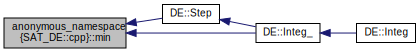
\includegraphics[width=350pt]{namespaceanonymous__namespace_02SAT__DE_8cpp_03_ae4ba4f69a40b68446f66e9f06a6df7c2_icgraph}
\end{center}
\end{figure}


\hypertarget{namespaceanonymous__namespace_02SAT__DE_8cpp_03_aabcae428edea4adc1bad5b1f9e9eb684}{\index{anonymous\-\_\-namespace\{\-S\-A\-T\-\_\-\-D\-E.\-cpp\}@{anonymous\-\_\-namespace\{\-S\-A\-T\-\_\-\-D\-E.\-cpp\}}!sign@{sign}}
\index{sign@{sign}!anonymous_namespace{SAT_DE.cpp}@{anonymous\-\_\-namespace\{\-S\-A\-T\-\_\-\-D\-E.\-cpp\}}}
\subsubsection[{sign}]{\setlength{\rightskip}{0pt plus 5cm}double anonymous\-\_\-namespace\{S\-A\-T\-\_\-\-D\-E.\-cpp\}\-::sign (
\begin{DoxyParamCaption}
\item[{double}]{a, }
\item[{double}]{b}
\end{DoxyParamCaption}
)}}\label{namespaceanonymous__namespace_02SAT__DE_8cpp_03_aabcae428edea4adc1bad5b1f9e9eb684}


Definition at line 74 of file S\-A\-T\-\_\-\-D\-E.\-cpp.



Here is the caller graph for this function\-:\nopagebreak
\begin{figure}[H]
\begin{center}
\leavevmode
\includegraphics[width=350pt]{namespaceanonymous__namespace_02SAT__DE_8cpp_03_aabcae428edea4adc1bad5b1f9e9eb684_icgraph}
\end{center}
\end{figure}




\subsection{Variable Documentation}
\hypertarget{namespaceanonymous__namespace_02SAT__DE_8cpp_03_a5299ad0fd8f5e34ef1ef5a2e5acdaa2c}{\index{anonymous\-\_\-namespace\{\-S\-A\-T\-\_\-\-D\-E.\-cpp\}@{anonymous\-\_\-namespace\{\-S\-A\-T\-\_\-\-D\-E.\-cpp\}}!fouru@{fouru}}
\index{fouru@{fouru}!anonymous_namespace{SAT_DE.cpp}@{anonymous\-\_\-namespace\{\-S\-A\-T\-\_\-\-D\-E.\-cpp\}}}
\subsubsection[{fouru}]{\setlength{\rightskip}{0pt plus 5cm}const double anonymous\-\_\-namespace\{S\-A\-T\-\_\-\-D\-E.\-cpp\}\-::fouru = 4.\-0$\ast${\bf umach}}}\label{namespaceanonymous__namespace_02SAT__DE_8cpp_03_a5299ad0fd8f5e34ef1ef5a2e5acdaa2c}


Definition at line 62 of file S\-A\-T\-\_\-\-D\-E.\-cpp.

\hypertarget{namespaceanonymous__namespace_02SAT__DE_8cpp_03_a0ed7041d585ca8647b8bff9a4d9d62e6}{\index{anonymous\-\_\-namespace\{\-S\-A\-T\-\_\-\-D\-E.\-cpp\}@{anonymous\-\_\-namespace\{\-S\-A\-T\-\_\-\-D\-E.\-cpp\}}!maxnum@{maxnum}}
\index{maxnum@{maxnum}!anonymous_namespace{SAT_DE.cpp}@{anonymous\-\_\-namespace\{\-S\-A\-T\-\_\-\-D\-E.\-cpp\}}}
\subsubsection[{maxnum}]{\setlength{\rightskip}{0pt plus 5cm}const int anonymous\-\_\-namespace\{S\-A\-T\-\_\-\-D\-E.\-cpp\}\-::maxnum = 500}}\label{namespaceanonymous__namespace_02SAT__DE_8cpp_03_a0ed7041d585ca8647b8bff9a4d9d62e6}


Definition at line 54 of file S\-A\-T\-\_\-\-D\-E.\-cpp.

\hypertarget{namespaceanonymous__namespace_02SAT__DE_8cpp_03_ac7d697ccca057a8340590bebf83de9f7}{\index{anonymous\-\_\-namespace\{\-S\-A\-T\-\_\-\-D\-E.\-cpp\}@{anonymous\-\_\-namespace\{\-S\-A\-T\-\_\-\-D\-E.\-cpp\}}!twou@{twou}}
\index{twou@{twou}!anonymous_namespace{SAT_DE.cpp}@{anonymous\-\_\-namespace\{\-S\-A\-T\-\_\-\-D\-E.\-cpp\}}}
\subsubsection[{twou}]{\setlength{\rightskip}{0pt plus 5cm}const double anonymous\-\_\-namespace\{S\-A\-T\-\_\-\-D\-E.\-cpp\}\-::twou = 2.\-0$\ast${\bf umach}}}\label{namespaceanonymous__namespace_02SAT__DE_8cpp_03_ac7d697ccca057a8340590bebf83de9f7}


Definition at line 61 of file S\-A\-T\-\_\-\-D\-E.\-cpp.

\hypertarget{namespaceanonymous__namespace_02SAT__DE_8cpp_03_af9ba43b60b8cf661784a1b5c2410045d}{\index{anonymous\-\_\-namespace\{\-S\-A\-T\-\_\-\-D\-E.\-cpp\}@{anonymous\-\_\-namespace\{\-S\-A\-T\-\_\-\-D\-E.\-cpp\}}!umach@{umach}}
\index{umach@{umach}!anonymous_namespace{SAT_DE.cpp}@{anonymous\-\_\-namespace\{\-S\-A\-T\-\_\-\-D\-E.\-cpp\}}}
\subsubsection[{umach}]{\setlength{\rightskip}{0pt plus 5cm}const double anonymous\-\_\-namespace\{S\-A\-T\-\_\-\-D\-E.\-cpp\}\-::umach = std\-::numeric\-\_\-limits$<$double$>$\-::epsilon()}}\label{namespaceanonymous__namespace_02SAT__DE_8cpp_03_af9ba43b60b8cf661784a1b5c2410045d}


Definition at line 59 of file S\-A\-T\-\_\-\-D\-E.\-cpp.


\hypertarget{namespaceanonymous__namespace_02SAT__Force_8cpp_03}{\section{anonymous\-\_\-namespace\{S\-A\-T\-\_\-\-Force.\-cpp\} Namespace Reference}
\label{namespaceanonymous__namespace_02SAT__Force_8cpp_03}\index{anonymous\-\_\-namespace\{\-S\-A\-T\-\_\-\-Force.\-cpp\}@{anonymous\-\_\-namespace\{\-S\-A\-T\-\_\-\-Force.\-cpp\}}}
}
\subsection*{Functions}
\begin{DoxyCompactItemize}
\item 
double \hyperlink{namespaceanonymous__namespace_02SAT__Force_8cpp_03_aa6826b33621fa6ff5736c6432c487c1a}{Frac} (double x)
\end{DoxyCompactItemize}
\subsection*{Variables}
\begin{DoxyCompactItemize}
\item 
const double \hyperlink{namespaceanonymous__namespace_02SAT__Force_8cpp_03_adc98a306a4a3c40934f207108c4f2d3a}{R\-\_\-\-J\-G\-M3} = 6378.\-1363e3
\item 
const int \hyperlink{namespaceanonymous__namespace_02SAT__Force_8cpp_03_a21c47b295844aa01ef36e5769862e2a3}{N\-\_\-\-J\-G\-M3} = 20
\item 
const double \hyperlink{namespaceanonymous__namespace_02SAT__Force_8cpp_03_a5d47d698acd0c2506ccfc42cdc162bf7}{C\-S\-\_\-\-J\-G\-M3} \mbox{[}\hyperlink{namespaceanonymous__namespace_02SAT__Force_8cpp_03_a21c47b295844aa01ef36e5769862e2a3}{N\-\_\-\-J\-G\-M3}+1\mbox{]}\mbox{[}\hyperlink{namespaceanonymous__namespace_02SAT__Force_8cpp_03_a21c47b295844aa01ef36e5769862e2a3}{N\-\_\-\-J\-G\-M3}+1\mbox{]}
\end{DoxyCompactItemize}


\subsection{Function Documentation}
\hypertarget{namespaceanonymous__namespace_02SAT__Force_8cpp_03_aa6826b33621fa6ff5736c6432c487c1a}{\index{anonymous\-\_\-namespace\{\-S\-A\-T\-\_\-\-Force.\-cpp\}@{anonymous\-\_\-namespace\{\-S\-A\-T\-\_\-\-Force.\-cpp\}}!Frac@{Frac}}
\index{Frac@{Frac}!anonymous_namespace{SAT_Force.cpp}@{anonymous\-\_\-namespace\{\-S\-A\-T\-\_\-\-Force.\-cpp\}}}
\subsubsection[{Frac}]{\setlength{\rightskip}{0pt plus 5cm}double anonymous\-\_\-namespace\{S\-A\-T\-\_\-\-Force.\-cpp\}\-::Frac (
\begin{DoxyParamCaption}
\item[{double}]{x}
\end{DoxyParamCaption}
)}}\label{namespaceanonymous__namespace_02SAT__Force_8cpp_03_aa6826b33621fa6ff5736c6432c487c1a}


Definition at line 48 of file S\-A\-T\-\_\-\-Force.\-cpp.



Here is the caller graph for this function\-:\nopagebreak
\begin{figure}[H]
\begin{center}
\leavevmode
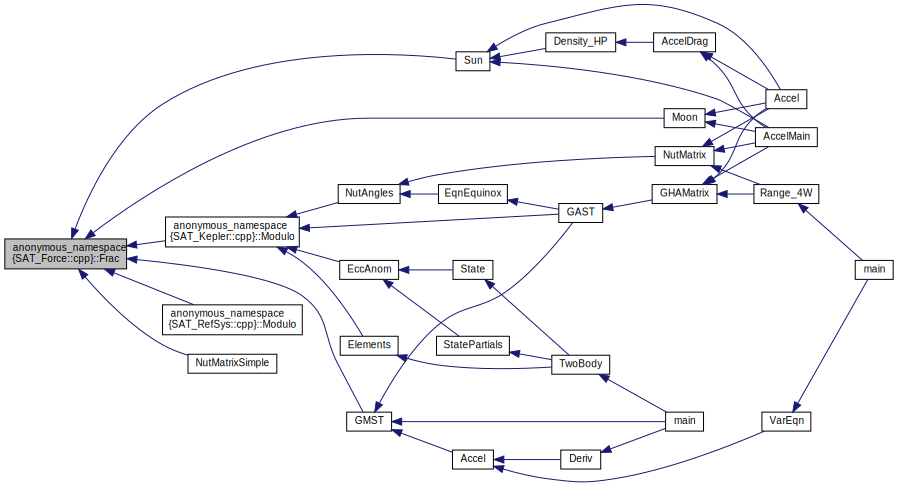
\includegraphics[width=350pt]{namespaceanonymous__namespace_02SAT__Force_8cpp_03_aa6826b33621fa6ff5736c6432c487c1a_icgraph}
\end{center}
\end{figure}




\subsection{Variable Documentation}
\hypertarget{namespaceanonymous__namespace_02SAT__Force_8cpp_03_a5d47d698acd0c2506ccfc42cdc162bf7}{\index{anonymous\-\_\-namespace\{\-S\-A\-T\-\_\-\-Force.\-cpp\}@{anonymous\-\_\-namespace\{\-S\-A\-T\-\_\-\-Force.\-cpp\}}!C\-S\-\_\-\-J\-G\-M3@{C\-S\-\_\-\-J\-G\-M3}}
\index{C\-S\-\_\-\-J\-G\-M3@{C\-S\-\_\-\-J\-G\-M3}!anonymous_namespace{SAT_Force.cpp}@{anonymous\-\_\-namespace\{\-S\-A\-T\-\_\-\-Force.\-cpp\}}}
\subsubsection[{C\-S\-\_\-\-J\-G\-M3}]{\setlength{\rightskip}{0pt plus 5cm}const double anonymous\-\_\-namespace\{S\-A\-T\-\_\-\-Force.\-cpp\}\-::C\-S\-\_\-\-J\-G\-M3\mbox{[}{\bf N\-\_\-\-J\-G\-M3}+1\mbox{]}\mbox{[}{\bf N\-\_\-\-J\-G\-M3}+1\mbox{]}}}\label{namespaceanonymous__namespace_02SAT__Force_8cpp_03_a5d47d698acd0c2506ccfc42cdc162bf7}


Definition at line 62 of file S\-A\-T\-\_\-\-Force.\-cpp.

\hypertarget{namespaceanonymous__namespace_02SAT__Force_8cpp_03_a21c47b295844aa01ef36e5769862e2a3}{\index{anonymous\-\_\-namespace\{\-S\-A\-T\-\_\-\-Force.\-cpp\}@{anonymous\-\_\-namespace\{\-S\-A\-T\-\_\-\-Force.\-cpp\}}!N\-\_\-\-J\-G\-M3@{N\-\_\-\-J\-G\-M3}}
\index{N\-\_\-\-J\-G\-M3@{N\-\_\-\-J\-G\-M3}!anonymous_namespace{SAT_Force.cpp}@{anonymous\-\_\-namespace\{\-S\-A\-T\-\_\-\-Force.\-cpp\}}}
\subsubsection[{N\-\_\-\-J\-G\-M3}]{\setlength{\rightskip}{0pt plus 5cm}const int anonymous\-\_\-namespace\{S\-A\-T\-\_\-\-Force.\-cpp\}\-::N\-\_\-\-J\-G\-M3 = 20}}\label{namespaceanonymous__namespace_02SAT__Force_8cpp_03_a21c47b295844aa01ef36e5769862e2a3}


Definition at line 61 of file S\-A\-T\-\_\-\-Force.\-cpp.

\hypertarget{namespaceanonymous__namespace_02SAT__Force_8cpp_03_adc98a306a4a3c40934f207108c4f2d3a}{\index{anonymous\-\_\-namespace\{\-S\-A\-T\-\_\-\-Force.\-cpp\}@{anonymous\-\_\-namespace\{\-S\-A\-T\-\_\-\-Force.\-cpp\}}!R\-\_\-\-J\-G\-M3@{R\-\_\-\-J\-G\-M3}}
\index{R\-\_\-\-J\-G\-M3@{R\-\_\-\-J\-G\-M3}!anonymous_namespace{SAT_Force.cpp}@{anonymous\-\_\-namespace\{\-S\-A\-T\-\_\-\-Force.\-cpp\}}}
\subsubsection[{R\-\_\-\-J\-G\-M3}]{\setlength{\rightskip}{0pt plus 5cm}const double anonymous\-\_\-namespace\{S\-A\-T\-\_\-\-Force.\-cpp\}\-::R\-\_\-\-J\-G\-M3 = 6378.\-1363e3}}\label{namespaceanonymous__namespace_02SAT__Force_8cpp_03_adc98a306a4a3c40934f207108c4f2d3a}


Definition at line 60 of file S\-A\-T\-\_\-\-Force.\-cpp.


\hypertarget{namespaceanonymous__namespace_02SAT__Kepler_8cpp_03}{\section{anonymous\-\_\-namespace\{S\-A\-T\-\_\-\-Kepler.\-cpp\} Namespace Reference}
\label{namespaceanonymous__namespace_02SAT__Kepler_8cpp_03}\index{anonymous\-\_\-namespace\{\-S\-A\-T\-\_\-\-Kepler.\-cpp\}@{anonymous\-\_\-namespace\{\-S\-A\-T\-\_\-\-Kepler.\-cpp\}}}
}
\subsection*{Functions}
\begin{DoxyCompactItemize}
\item 
double \hyperlink{namespaceanonymous__namespace_02SAT__Kepler_8cpp_03_aa49f9f9ad3a8153f0982dc37fe17c4f2}{Frac} (double x)
\item 
double \hyperlink{namespaceanonymous__namespace_02SAT__Kepler_8cpp_03_ae5d42531d691a174363f296c22d23217}{Modulo} (double x, double y)
\item 
double \hyperlink{namespaceanonymous__namespace_02SAT__Kepler_8cpp_03_a898091d856dff0d563448625b7634f16}{F} (double eta, double m, double l)
\end{DoxyCompactItemize}
\subsection*{Variables}
\begin{DoxyCompactItemize}
\item 
const double \hyperlink{namespaceanonymous__namespace_02SAT__Kepler_8cpp_03_a4a19f0e7912b0c72da53321784af4b1b}{eps\-\_\-mach} = std\-::numeric\-\_\-limits$<$double$>$\-::epsilon()
\end{DoxyCompactItemize}


\subsection{Function Documentation}
\hypertarget{namespaceanonymous__namespace_02SAT__Kepler_8cpp_03_a898091d856dff0d563448625b7634f16}{\index{anonymous\-\_\-namespace\{\-S\-A\-T\-\_\-\-Kepler.\-cpp\}@{anonymous\-\_\-namespace\{\-S\-A\-T\-\_\-\-Kepler.\-cpp\}}!F@{F}}
\index{F@{F}!anonymous_namespace{SAT_Kepler.cpp}@{anonymous\-\_\-namespace\{\-S\-A\-T\-\_\-\-Kepler.\-cpp\}}}
\subsubsection[{F}]{\setlength{\rightskip}{0pt plus 5cm}double anonymous\-\_\-namespace\{S\-A\-T\-\_\-\-Kepler.\-cpp\}\-::F (
\begin{DoxyParamCaption}
\item[{double}]{eta, }
\item[{double}]{m, }
\item[{double}]{l}
\end{DoxyParamCaption}
)}}\label{namespaceanonymous__namespace_02SAT__Kepler_8cpp_03_a898091d856dff0d563448625b7634f16}


Definition at line 78 of file S\-A\-T\-\_\-\-Kepler.\-cpp.



Here is the caller graph for this function\-:\nopagebreak
\begin{figure}[H]
\begin{center}
\leavevmode
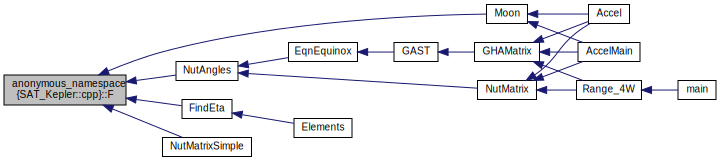
\includegraphics[width=350pt]{namespaceanonymous__namespace_02SAT__Kepler_8cpp_03_a898091d856dff0d563448625b7634f16_icgraph}
\end{center}
\end{figure}


\hypertarget{namespaceanonymous__namespace_02SAT__Kepler_8cpp_03_aa49f9f9ad3a8153f0982dc37fe17c4f2}{\index{anonymous\-\_\-namespace\{\-S\-A\-T\-\_\-\-Kepler.\-cpp\}@{anonymous\-\_\-namespace\{\-S\-A\-T\-\_\-\-Kepler.\-cpp\}}!Frac@{Frac}}
\index{Frac@{Frac}!anonymous_namespace{SAT_Kepler.cpp}@{anonymous\-\_\-namespace\{\-S\-A\-T\-\_\-\-Kepler.\-cpp\}}}
\subsubsection[{Frac}]{\setlength{\rightskip}{0pt plus 5cm}double anonymous\-\_\-namespace\{S\-A\-T\-\_\-\-Kepler.\-cpp\}\-::Frac (
\begin{DoxyParamCaption}
\item[{double}]{x}
\end{DoxyParamCaption}
)}}\label{namespaceanonymous__namespace_02SAT__Kepler_8cpp_03_aa49f9f9ad3a8153f0982dc37fe17c4f2}


Definition at line 65 of file S\-A\-T\-\_\-\-Kepler.\-cpp.

\hypertarget{namespaceanonymous__namespace_02SAT__Kepler_8cpp_03_ae5d42531d691a174363f296c22d23217}{\index{anonymous\-\_\-namespace\{\-S\-A\-T\-\_\-\-Kepler.\-cpp\}@{anonymous\-\_\-namespace\{\-S\-A\-T\-\_\-\-Kepler.\-cpp\}}!Modulo@{Modulo}}
\index{Modulo@{Modulo}!anonymous_namespace{SAT_Kepler.cpp}@{anonymous\-\_\-namespace\{\-S\-A\-T\-\_\-\-Kepler.\-cpp\}}}
\subsubsection[{Modulo}]{\setlength{\rightskip}{0pt plus 5cm}double anonymous\-\_\-namespace\{S\-A\-T\-\_\-\-Kepler.\-cpp\}\-::Modulo (
\begin{DoxyParamCaption}
\item[{double}]{x, }
\item[{double}]{y}
\end{DoxyParamCaption}
)}}\label{namespaceanonymous__namespace_02SAT__Kepler_8cpp_03_ae5d42531d691a174363f296c22d23217}


Definition at line 71 of file S\-A\-T\-\_\-\-Kepler.\-cpp.



Here is the call graph for this function\-:\nopagebreak
\begin{figure}[H]
\begin{center}
\leavevmode
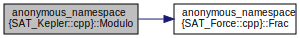
\includegraphics[width=350pt]{namespaceanonymous__namespace_02SAT__Kepler_8cpp_03_ae5d42531d691a174363f296c22d23217_cgraph}
\end{center}
\end{figure}




Here is the caller graph for this function\-:\nopagebreak
\begin{figure}[H]
\begin{center}
\leavevmode
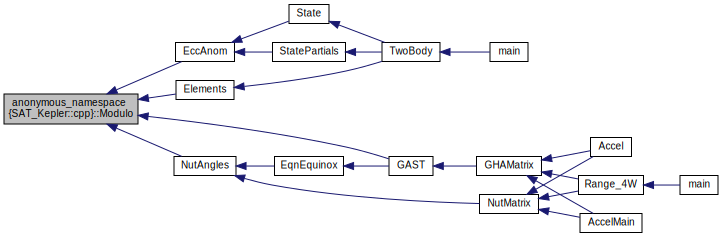
\includegraphics[width=350pt]{namespaceanonymous__namespace_02SAT__Kepler_8cpp_03_ae5d42531d691a174363f296c22d23217_icgraph}
\end{center}
\end{figure}




\subsection{Variable Documentation}
\hypertarget{namespaceanonymous__namespace_02SAT__Kepler_8cpp_03_a4a19f0e7912b0c72da53321784af4b1b}{\index{anonymous\-\_\-namespace\{\-S\-A\-T\-\_\-\-Kepler.\-cpp\}@{anonymous\-\_\-namespace\{\-S\-A\-T\-\_\-\-Kepler.\-cpp\}}!eps\-\_\-mach@{eps\-\_\-mach}}
\index{eps\-\_\-mach@{eps\-\_\-mach}!anonymous_namespace{SAT_Kepler.cpp}@{anonymous\-\_\-namespace\{\-S\-A\-T\-\_\-\-Kepler.\-cpp\}}}
\subsubsection[{eps\-\_\-mach}]{\setlength{\rightskip}{0pt plus 5cm}const double anonymous\-\_\-namespace\{S\-A\-T\-\_\-\-Kepler.\-cpp\}\-::eps\-\_\-mach = std\-::numeric\-\_\-limits$<$double$>$\-::epsilon()}}\label{namespaceanonymous__namespace_02SAT__Kepler_8cpp_03_a4a19f0e7912b0c72da53321784af4b1b}


Definition at line 58 of file S\-A\-T\-\_\-\-Kepler.\-cpp.


\hypertarget{namespaceanonymous__namespace_02SAT__RefSys_8cpp_03}{\section{anonymous\-\_\-namespace\{S\-A\-T\-\_\-\-Ref\-Sys.\-cpp\} Namespace Reference}
\label{namespaceanonymous__namespace_02SAT__RefSys_8cpp_03}\index{anonymous\-\_\-namespace\{\-S\-A\-T\-\_\-\-Ref\-Sys.\-cpp\}@{anonymous\-\_\-namespace\{\-S\-A\-T\-\_\-\-Ref\-Sys.\-cpp\}}}
}
\subsection*{Functions}
\begin{DoxyCompactItemize}
\item 
double \hyperlink{namespaceanonymous__namespace_02SAT__RefSys_8cpp_03_a8aadb7444f7d4876ac56668e643d5ec4}{Frac} (double x)
\item 
double \hyperlink{namespaceanonymous__namespace_02SAT__RefSys_8cpp_03_a8369415c3f0725f627fbb5db1676becc}{Modulo} (double x, double y)
\end{DoxyCompactItemize}
\subsection*{Variables}
\begin{DoxyCompactItemize}
\item 
const double \hyperlink{namespaceanonymous__namespace_02SAT__RefSys_8cpp_03_a0e9503fdab61b8a184fe4940ef37e590}{eps\-\_\-mach} = std\-::numeric\-\_\-limits$<$double$>$\-::epsilon()
\end{DoxyCompactItemize}


\subsection{Function Documentation}
\hypertarget{namespaceanonymous__namespace_02SAT__RefSys_8cpp_03_a8aadb7444f7d4876ac56668e643d5ec4}{\index{anonymous\-\_\-namespace\{\-S\-A\-T\-\_\-\-Ref\-Sys.\-cpp\}@{anonymous\-\_\-namespace\{\-S\-A\-T\-\_\-\-Ref\-Sys.\-cpp\}}!Frac@{Frac}}
\index{Frac@{Frac}!anonymous_namespace{SAT_RefSys.cpp}@{anonymous\-\_\-namespace\{\-S\-A\-T\-\_\-\-Ref\-Sys.\-cpp\}}}
\subsubsection[{Frac}]{\setlength{\rightskip}{0pt plus 5cm}double anonymous\-\_\-namespace\{S\-A\-T\-\_\-\-Ref\-Sys.\-cpp\}\-::Frac (
\begin{DoxyParamCaption}
\item[{double}]{x}
\end{DoxyParamCaption}
)}}\label{namespaceanonymous__namespace_02SAT__RefSys_8cpp_03_a8aadb7444f7d4876ac56668e643d5ec4}


Definition at line 60 of file S\-A\-T\-\_\-\-Ref\-Sys.\-cpp.

\hypertarget{namespaceanonymous__namespace_02SAT__RefSys_8cpp_03_a8369415c3f0725f627fbb5db1676becc}{\index{anonymous\-\_\-namespace\{\-S\-A\-T\-\_\-\-Ref\-Sys.\-cpp\}@{anonymous\-\_\-namespace\{\-S\-A\-T\-\_\-\-Ref\-Sys.\-cpp\}}!Modulo@{Modulo}}
\index{Modulo@{Modulo}!anonymous_namespace{SAT_RefSys.cpp}@{anonymous\-\_\-namespace\{\-S\-A\-T\-\_\-\-Ref\-Sys.\-cpp\}}}
\subsubsection[{Modulo}]{\setlength{\rightskip}{0pt plus 5cm}double anonymous\-\_\-namespace\{S\-A\-T\-\_\-\-Ref\-Sys.\-cpp\}\-::Modulo (
\begin{DoxyParamCaption}
\item[{double}]{x, }
\item[{double}]{y}
\end{DoxyParamCaption}
)}}\label{namespaceanonymous__namespace_02SAT__RefSys_8cpp_03_a8369415c3f0725f627fbb5db1676becc}


Definition at line 62 of file S\-A\-T\-\_\-\-Ref\-Sys.\-cpp.



Here is the call graph for this function\-:\nopagebreak
\begin{figure}[H]
\begin{center}
\leavevmode
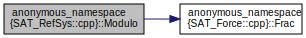
\includegraphics[width=350pt]{namespaceanonymous__namespace_02SAT__RefSys_8cpp_03_a8369415c3f0725f627fbb5db1676becc_cgraph}
\end{center}
\end{figure}




\subsection{Variable Documentation}
\hypertarget{namespaceanonymous__namespace_02SAT__RefSys_8cpp_03_a0e9503fdab61b8a184fe4940ef37e590}{\index{anonymous\-\_\-namespace\{\-S\-A\-T\-\_\-\-Ref\-Sys.\-cpp\}@{anonymous\-\_\-namespace\{\-S\-A\-T\-\_\-\-Ref\-Sys.\-cpp\}}!eps\-\_\-mach@{eps\-\_\-mach}}
\index{eps\-\_\-mach@{eps\-\_\-mach}!anonymous_namespace{SAT_RefSys.cpp}@{anonymous\-\_\-namespace\{\-S\-A\-T\-\_\-\-Ref\-Sys.\-cpp\}}}
\subsubsection[{eps\-\_\-mach}]{\setlength{\rightskip}{0pt plus 5cm}const double anonymous\-\_\-namespace\{S\-A\-T\-\_\-\-Ref\-Sys.\-cpp\}\-::eps\-\_\-mach = std\-::numeric\-\_\-limits$<$double$>$\-::epsilon()}}\label{namespaceanonymous__namespace_02SAT__RefSys_8cpp_03_a0e9503fdab61b8a184fe4940ef37e590}


Definition at line 57 of file S\-A\-T\-\_\-\-Ref\-Sys.\-cpp.


\chapter{Class Documentation}
\hypertarget{structAuxParam}{\section{Aux\-Param Struct Reference}
\label{structAuxParam}\index{Aux\-Param@{Aux\-Param}}
}
\subsection*{Public Attributes}
\begin{DoxyCompactItemize}
\item 
double \hyperlink{structAuxParam_ac11f26de5fc55f2ae6fa20349290be18}{Mjd0\-\_\-\-G\-P\-S}
\item 
int \hyperlink{structAuxParam_a18fb836f348b92544dc701bb831ab366}{n\-\_\-grav}
\item 
double \hyperlink{structAuxParam_a57f18ab074819216ae0dcc8d4966e636}{Mjd0\-\_\-\-T\-T}
\item 
double \hyperlink{structAuxParam_abcebf1a69b5a06b594f99e39c79b4a47}{Area}
\item 
double \hyperlink{structAuxParam_afb25e5df632f3a7ba7b18755dcad08ad}{mass}
\item 
double \hyperlink{structAuxParam_ab3aad49adad1f5abe376ef54d87a5564}{C\-R}
\item 
double \hyperlink{structAuxParam_af83c855c2c9a458df9fb34c0aa20c1fc}{C\-D}
\end{DoxyCompactItemize}


\subsection{Detailed Description}


Definition at line 67 of file R\-T\-O\-D.\-cpp.



\subsection{Member Data Documentation}
\hypertarget{structAuxParam_abcebf1a69b5a06b594f99e39c79b4a47}{\index{Aux\-Param@{Aux\-Param}!Area@{Area}}
\index{Area@{Area}!AuxParam@{Aux\-Param}}
\subsubsection[{Area}]{\setlength{\rightskip}{0pt plus 5cm}double Aux\-Param\-::\-Area}}\label{structAuxParam_abcebf1a69b5a06b594f99e39c79b4a47}


Definition at line 76 of file T\-D\-R\-S\-O\-D.\-cpp.

\hypertarget{structAuxParam_af83c855c2c9a458df9fb34c0aa20c1fc}{\index{Aux\-Param@{Aux\-Param}!C\-D@{C\-D}}
\index{C\-D@{C\-D}!AuxParam@{Aux\-Param}}
\subsubsection[{C\-D}]{\setlength{\rightskip}{0pt plus 5cm}double Aux\-Param\-::\-C\-D}}\label{structAuxParam_af83c855c2c9a458df9fb34c0aa20c1fc}


Definition at line 77 of file T\-D\-R\-S\-O\-D.\-cpp.

\hypertarget{structAuxParam_ab3aad49adad1f5abe376ef54d87a5564}{\index{Aux\-Param@{Aux\-Param}!C\-R@{C\-R}}
\index{C\-R@{C\-R}!AuxParam@{Aux\-Param}}
\subsubsection[{C\-R}]{\setlength{\rightskip}{0pt plus 5cm}double Aux\-Param\-::\-C\-R}}\label{structAuxParam_ab3aad49adad1f5abe376ef54d87a5564}


Definition at line 77 of file T\-D\-R\-S\-O\-D.\-cpp.

\hypertarget{structAuxParam_afb25e5df632f3a7ba7b18755dcad08ad}{\index{Aux\-Param@{Aux\-Param}!mass@{mass}}
\index{mass@{mass}!AuxParam@{Aux\-Param}}
\subsubsection[{mass}]{\setlength{\rightskip}{0pt plus 5cm}double Aux\-Param\-::mass}}\label{structAuxParam_afb25e5df632f3a7ba7b18755dcad08ad}


Definition at line 76 of file T\-D\-R\-S\-O\-D.\-cpp.

\hypertarget{structAuxParam_ac11f26de5fc55f2ae6fa20349290be18}{\index{Aux\-Param@{Aux\-Param}!Mjd0\-\_\-\-G\-P\-S@{Mjd0\-\_\-\-G\-P\-S}}
\index{Mjd0\-\_\-\-G\-P\-S@{Mjd0\-\_\-\-G\-P\-S}!AuxParam@{Aux\-Param}}
\subsubsection[{Mjd0\-\_\-\-G\-P\-S}]{\setlength{\rightskip}{0pt plus 5cm}double Aux\-Param\-::\-Mjd0\-\_\-\-G\-P\-S}}\label{structAuxParam_ac11f26de5fc55f2ae6fa20349290be18}


Definition at line 68 of file R\-T\-O\-D.\-cpp.

\hypertarget{structAuxParam_a57f18ab074819216ae0dcc8d4966e636}{\index{Aux\-Param@{Aux\-Param}!Mjd0\-\_\-\-T\-T@{Mjd0\-\_\-\-T\-T}}
\index{Mjd0\-\_\-\-T\-T@{Mjd0\-\_\-\-T\-T}!AuxParam@{Aux\-Param}}
\subsubsection[{Mjd0\-\_\-\-T\-T}]{\setlength{\rightskip}{0pt plus 5cm}double Aux\-Param\-::\-Mjd0\-\_\-\-T\-T}}\label{structAuxParam_a57f18ab074819216ae0dcc8d4966e636}


Definition at line 75 of file T\-D\-R\-S\-O\-D.\-cpp.

\hypertarget{structAuxParam_a18fb836f348b92544dc701bb831ab366}{\index{Aux\-Param@{Aux\-Param}!n\-\_\-grav@{n\-\_\-grav}}
\index{n\-\_\-grav@{n\-\_\-grav}!AuxParam@{Aux\-Param}}
\subsubsection[{n\-\_\-grav}]{\setlength{\rightskip}{0pt plus 5cm}int Aux\-Param\-::n\-\_\-grav}}\label{structAuxParam_a18fb836f348b92544dc701bb831ab366}


Definition at line 69 of file R\-T\-O\-D.\-cpp.



The documentation for this struct was generated from the following files\-:\begin{DoxyCompactItemize}
\item 
\hyperlink{RTOD_8cpp}{R\-T\-O\-D.\-cpp}\item 
\hyperlink{TDRSOD_8cpp}{T\-D\-R\-S\-O\-D.\-cpp}\end{DoxyCompactItemize}

\hypertarget{classDate}{\section{Date Class Reference}
\label{classDate}\index{Date@{Date}}
}


{\ttfamily \#include $<$S\-A\-T\-\_\-\-Time.\-h$>$}

\subsection*{Public Member Functions}
\begin{DoxyCompactItemize}
\item 
\hyperlink{classDate_a6f9bfcf22a1de071ae7bca7f88b36944}{Date} (double \hyperlink{SAT__Time_8h_aff6573e3bb353cea8fc54ff4995365cd}{Mjd})
\end{DoxyCompactItemize}
\subsection*{Private Attributes}
\begin{DoxyCompactItemize}
\item 
double \hyperlink{classDate_adcb18582f8f21a09e65e28f60bf01bcd}{mjd}
\end{DoxyCompactItemize}
\subsection*{Friends}
\begin{DoxyCompactItemize}
\item 
std\-::ostream \& \hyperlink{classDate_a61392cf9bd721b5649cf5d2fbfa4e84b}{operator$<$$<$} (std\-::ostream \&os, const \hyperlink{classDate}{Date} \&D)
\end{DoxyCompactItemize}


\subsection{Detailed Description}


Definition at line 94 of file S\-A\-T\-\_\-\-Time.\-h.



\subsection{Constructor \& Destructor Documentation}
\hypertarget{classDate_a6f9bfcf22a1de071ae7bca7f88b36944}{\index{Date@{Date}!Date@{Date}}
\index{Date@{Date}!Date@{Date}}
\subsubsection[{Date}]{\setlength{\rightskip}{0pt plus 5cm}Date\-::\-Date (
\begin{DoxyParamCaption}
\item[{double}]{Mjd}
\end{DoxyParamCaption}
)}}\label{classDate_a6f9bfcf22a1de071ae7bca7f88b36944}


Definition at line 151 of file S\-A\-T\-\_\-\-Time.\-cpp.



\subsection{Friends And Related Function Documentation}
\hypertarget{classDate_a61392cf9bd721b5649cf5d2fbfa4e84b}{\index{Date@{Date}!operator$<$$<$@{operator$<$$<$}}
\index{operator$<$$<$@{operator$<$$<$}!Date@{Date}}
\subsubsection[{operator$<$$<$}]{\setlength{\rightskip}{0pt plus 5cm}std\-::ostream\& operator$<$$<$ (
\begin{DoxyParamCaption}
\item[{std\-::ostream \&}]{os, }
\item[{const {\bf Date} \&}]{D}
\end{DoxyParamCaption}
)\hspace{0.3cm}{\ttfamily [friend]}}}\label{classDate_a61392cf9bd721b5649cf5d2fbfa4e84b}


\subsection{Member Data Documentation}
\hypertarget{classDate_adcb18582f8f21a09e65e28f60bf01bcd}{\index{Date@{Date}!mjd@{mjd}}
\index{mjd@{mjd}!Date@{Date}}
\subsubsection[{mjd}]{\setlength{\rightskip}{0pt plus 5cm}double Date\-::mjd\hspace{0.3cm}{\ttfamily [private]}}}\label{classDate_adcb18582f8f21a09e65e28f60bf01bcd}


Definition at line 100 of file S\-A\-T\-\_\-\-Time.\-h.



The documentation for this class was generated from the following files\-:\begin{DoxyCompactItemize}
\item 
\hyperlink{SAT__Time_8h}{S\-A\-T\-\_\-\-Time.\-h}\item 
\hyperlink{SAT__Time_8cpp}{S\-A\-T\-\_\-\-Time.\-cpp}\end{DoxyCompactItemize}

\hypertarget{classDE}{\section{D\-E Class Reference}
\label{classDE}\index{D\-E@{D\-E}}
}


{\ttfamily \#include $<$S\-A\-T\-\_\-\-D\-E.\-h$>$}



Collaboration diagram for D\-E\-:\nopagebreak
\begin{figure}[H]
\begin{center}
\leavevmode
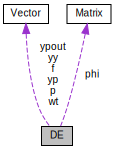
\includegraphics[width=187pt]{classDE__coll__graph}
\end{center}
\end{figure}
\subsection*{Public Member Functions}
\begin{DoxyCompactItemize}
\item 
\hyperlink{classDE_a37d9ef0ccffda10dda67b29538416d0c}{D\-E} ()
\item 
\hyperlink{classDE_a6b0641c47ad6a3d42f04d08583e6839d}{D\-E} (\hyperlink{SAT__DE_8h_a37c3f0fc3c33a5b858a3f1c90353da48}{D\-Efunct} f\-\_\-, int n\-\_\-eqn\-\_\-, void $\ast$p\-Aux\-\_\-)
\item 
void \hyperlink{classDE_a1eebc6bc641f0f375e6077f0404fc1e0}{Define} (\hyperlink{SAT__DE_8h_a37c3f0fc3c33a5b858a3f1c90353da48}{D\-Efunct} f\-\_\-, int n\-\_\-eqn\-\_\-, void $\ast$p\-Aux\-\_\-)
\item 
void \hyperlink{classDE_a2cedbf51ef4121e63b3c4578df6b3905}{Init} (double t0, double rel, double abs)
\item 
void \hyperlink{classDE_a6a008818dc6d8ad8defd822091207093}{Integ} (double tout, \hyperlink{classVector}{Vector} \&y)
\item 
void \hyperlink{classDE_ada59157cf555a77f65242c04ad1c9e19}{Intrp} (double tout, \hyperlink{classVector}{Vector} \&y)
\end{DoxyCompactItemize}
\subsection*{Public Attributes}
\begin{DoxyCompactItemize}
\item 
double \hyperlink{classDE_a877edbd8bd4ba297b5602786b552059f}{relerr}
\item 
double \hyperlink{classDE_a9337b177c5adfeda779ceecd6b56b370}{abserr}
\item 
\hyperlink{SAT__DE_8h_a57a5a4efb7b7add9bd828d85d9bb920d}{D\-E\-\_\-\-S\-T\-A\-T\-E} \hyperlink{classDE_a1d99a54650b09e8192bf89537f66bed2}{State}
\item 
bool \hyperlink{classDE_ab4adac8a112f4c5b5600986b418e5129}{Permit\-T\-O\-U\-T}
\item 
double \hyperlink{classDE_a56ee5af65170db9321a5508c207cd173}{t}
\end{DoxyCompactItemize}
\subsection*{Private Member Functions}
\begin{DoxyCompactItemize}
\item 
void \hyperlink{classDE_ac45486f7c7bf422c6bd024aba501a2a2}{Step} (double \&\hyperlink{classDE_a53686f8f7ab89225ba80835e910168fa}{x}, \hyperlink{classVector}{Vector} \&y, double \&eps, bool \&crash)
\item 
void \hyperlink{classDE_a6437bef70b2bb04c1b041e6ea86665ad}{Intrp} (double xout, \hyperlink{classVector}{Vector} \&yout, \hyperlink{classVector}{Vector} \&\hyperlink{classDE_a985edfb71c582371040affbd4230a36a}{ypout})
\item 
void \hyperlink{classDE_ac5af669df33d23002a4744f0217e33dc}{Integ\-\_\-} (double \&\hyperlink{classDE_a56ee5af65170db9321a5508c207cd173}{t}, double tout, \hyperlink{classVector}{Vector} \&y)
\end{DoxyCompactItemize}
\subsection*{Private Attributes}
\begin{DoxyCompactItemize}
\item 
\hyperlink{SAT__DE_8h_a37c3f0fc3c33a5b858a3f1c90353da48}{D\-Efunct} \hyperlink{classDE_afa7fefa0ba10ee635a618b3a4a5a39dc}{f}
\item 
int \hyperlink{classDE_ae74a30c7f5448d96d8460b4fde65f849}{n\-\_\-eqn}
\item 
void $\ast$ \hyperlink{classDE_ab8fad10a55cec3f9755444ae5ee38903}{p\-Aux}
\item 
\hyperlink{classVector}{Vector} \hyperlink{classDE_ab501e078b2408ca63ee44c1c4d59de86}{yy}
\item 
\hyperlink{classVector}{Vector} \hyperlink{classDE_adc470cb3c810cd47c8603003f10d4cac}{wt}
\item 
\hyperlink{classVector}{Vector} \hyperlink{classDE_af16ce45fb590ddb2ae5225b5cfc95f87}{p}
\item 
\hyperlink{classVector}{Vector} \hyperlink{classDE_acff3aaf84faff7827daf981587ef5b03}{yp}
\item 
\hyperlink{classVector}{Vector} \hyperlink{classDE_a985edfb71c582371040affbd4230a36a}{ypout}
\item 
\hyperlink{classMatrix}{Matrix} \hyperlink{classDE_a79eb189fb7f3320d735b90ca3332311e}{phi}
\item 
double \hyperlink{classDE_ad0bf62cec063071d0773fde29d976c0e}{alpha} \mbox{[}13\mbox{]}
\item 
double \hyperlink{classDE_a6db4afe37f9ebf0dce0532415c40de32}{beta} \mbox{[}13\mbox{]}
\item 
double \hyperlink{classDE_af4b92bb3bf10322b581dbbcf778ef5d5}{v} \mbox{[}13\mbox{]}
\item 
double \hyperlink{classDE_a4cd9f3da02faec86f2926ce373a4e7c9}{w} \mbox{[}13\mbox{]}
\item 
double \hyperlink{classDE_a7ef55ab5c646e5f540adcfa6ed392b56}{psi} \mbox{[}13\mbox{]}
\item 
double \hyperlink{classDE_a2ec1db657ea1d2ba57e0221ca0cb3eef}{sig} \mbox{[}14\mbox{]}
\item 
double \hyperlink{classDE_aa5b66f7465475382f7f2d757fd9cf979}{g} \mbox{[}14\mbox{]}
\item 
double \hyperlink{classDE_a53686f8f7ab89225ba80835e910168fa}{x}
\item 
double \hyperlink{classDE_adcd1d27f91dc1de8c4e2e8572878f92f}{h}
\item 
double \hyperlink{classDE_a8aba1f4cf3cb574060e0772052b6772e}{hold}
\item 
double \hyperlink{classDE_a710c5e85925a2ce84f8d789c1b4cb99b}{told}
\item 
double \hyperlink{classDE_a5fe0648747453fc746c8bee223d58633}{delsgn}
\item 
int \hyperlink{classDE_a4d82322b4499d5f8e27f2e19675fcfa6}{ns}
\item 
int \hyperlink{classDE_a583b51553ddbe1eb995e76d42b2e13ec}{k}
\item 
int \hyperlink{classDE_aaa4409f0e1999d15aa33da045dcf464d}{kold}
\item 
bool \hyperlink{classDE_a210930a504af06e95856cb71411b2a6b}{Old\-Permit}
\item 
bool \hyperlink{classDE_ab9a2adeb8253f3901c1cb39387e35fba}{phase1}
\item 
bool \hyperlink{classDE_a3c9b03623043eee0c38ecefecf301320}{start}
\item 
bool \hyperlink{classDE_ab7d114c0f93009e0deddea4375764e52}{nornd}
\item 
bool \hyperlink{classDE_a992636687bf14328677c450008855770}{init}
\end{DoxyCompactItemize}


\subsection{Detailed Description}


Definition at line 126 of file S\-A\-T\-\_\-\-D\-E.\-h.



\subsection{Constructor \& Destructor Documentation}
\hypertarget{classDE_a37d9ef0ccffda10dda67b29538416d0c}{\index{D\-E@{D\-E}!D\-E@{D\-E}}
\index{D\-E@{D\-E}!DE@{D\-E}}
\subsubsection[{D\-E}]{\setlength{\rightskip}{0pt plus 5cm}D\-E\-::\-D\-E (
\begin{DoxyParamCaption}
{}
\end{DoxyParamCaption}
)}}\label{classDE_a37d9ef0ccffda10dda67b29538416d0c}


Definition at line 119 of file S\-A\-T\-\_\-\-D\-E.\-cpp.

\hypertarget{classDE_a6b0641c47ad6a3d42f04d08583e6839d}{\index{D\-E@{D\-E}!D\-E@{D\-E}}
\index{D\-E@{D\-E}!DE@{D\-E}}
\subsubsection[{D\-E}]{\setlength{\rightskip}{0pt plus 5cm}D\-E\-::\-D\-E (
\begin{DoxyParamCaption}
\item[{{\bf D\-Efunct}}]{f\-\_\-, }
\item[{int}]{n\-\_\-eqn\-\_\-, }
\item[{void $\ast$}]{p\-Aux\-\_\-}
\end{DoxyParamCaption}
)}}\label{classDE_a6b0641c47ad6a3d42f04d08583e6839d}


Definition at line 136 of file S\-A\-T\-\_\-\-D\-E.\-cpp.



\subsection{Member Function Documentation}
\hypertarget{classDE_a1eebc6bc641f0f375e6077f0404fc1e0}{\index{D\-E@{D\-E}!Define@{Define}}
\index{Define@{Define}!DE@{D\-E}}
\subsubsection[{Define}]{\setlength{\rightskip}{0pt plus 5cm}void D\-E\-::\-Define (
\begin{DoxyParamCaption}
\item[{{\bf D\-Efunct}}]{f\-\_\-, }
\item[{int}]{n\-\_\-eqn\-\_\-, }
\item[{void $\ast$}]{p\-Aux\-\_\-}
\end{DoxyParamCaption}
)}}\label{classDE_a1eebc6bc641f0f375e6077f0404fc1e0}


Definition at line 163 of file S\-A\-T\-\_\-\-D\-E.\-cpp.

\hypertarget{classDE_a2cedbf51ef4121e63b3c4578df6b3905}{\index{D\-E@{D\-E}!Init@{Init}}
\index{Init@{Init}!DE@{D\-E}}
\subsubsection[{Init}]{\setlength{\rightskip}{0pt plus 5cm}void D\-E\-::\-Init (
\begin{DoxyParamCaption}
\item[{double}]{t0, }
\item[{double}]{rel, }
\item[{double}]{abs}
\end{DoxyParamCaption}
)}}\label{classDE_a2cedbf51ef4121e63b3c4578df6b3905}


Definition at line 823 of file S\-A\-T\-\_\-\-D\-E.\-cpp.

\hypertarget{classDE_a6a008818dc6d8ad8defd822091207093}{\index{D\-E@{D\-E}!Integ@{Integ}}
\index{Integ@{Integ}!DE@{D\-E}}
\subsubsection[{Integ}]{\setlength{\rightskip}{0pt plus 5cm}void D\-E\-::\-Integ (
\begin{DoxyParamCaption}
\item[{double}]{tout, }
\item[{{\bf Vector} \&}]{y}
\end{DoxyParamCaption}
)}}\label{classDE_a6a008818dc6d8ad8defd822091207093}


Definition at line 841 of file S\-A\-T\-\_\-\-D\-E.\-cpp.



Here is the call graph for this function\-:\nopagebreak
\begin{figure}[H]
\begin{center}
\leavevmode
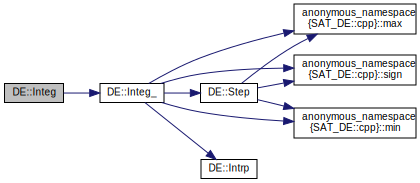
\includegraphics[width=350pt]{classDE_a6a008818dc6d8ad8defd822091207093_cgraph}
\end{center}
\end{figure}


\hypertarget{classDE_ac5af669df33d23002a4744f0217e33dc}{\index{D\-E@{D\-E}!Integ\-\_\-@{Integ\-\_\-}}
\index{Integ\-\_\-@{Integ\-\_\-}!DE@{D\-E}}
\subsubsection[{Integ\-\_\-}]{\setlength{\rightskip}{0pt plus 5cm}void D\-E\-::\-Integ\-\_\- (
\begin{DoxyParamCaption}
\item[{double \&}]{t, }
\item[{double}]{tout, }
\item[{{\bf Vector} \&}]{y}
\end{DoxyParamCaption}
)\hspace{0.3cm}{\ttfamily [private]}}}\label{classDE_ac5af669df33d23002a4744f0217e33dc}


Definition at line 686 of file S\-A\-T\-\_\-\-D\-E.\-cpp.



Here is the call graph for this function\-:\nopagebreak
\begin{figure}[H]
\begin{center}
\leavevmode
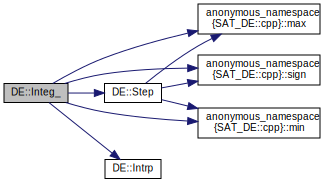
\includegraphics[width=350pt]{classDE_ac5af669df33d23002a4744f0217e33dc_cgraph}
\end{center}
\end{figure}




Here is the caller graph for this function\-:\nopagebreak
\begin{figure}[H]
\begin{center}
\leavevmode
\includegraphics[width=240pt]{classDE_ac5af669df33d23002a4744f0217e33dc_icgraph}
\end{center}
\end{figure}


\hypertarget{classDE_ada59157cf555a77f65242c04ad1c9e19}{\index{D\-E@{D\-E}!Intrp@{Intrp}}
\index{Intrp@{Intrp}!DE@{D\-E}}
\subsubsection[{Intrp}]{\setlength{\rightskip}{0pt plus 5cm}void D\-E\-::\-Intrp (
\begin{DoxyParamCaption}
\item[{double}]{tout, }
\item[{{\bf Vector} \&}]{y}
\end{DoxyParamCaption}
)}}\label{classDE_ada59157cf555a77f65242c04ad1c9e19}


Definition at line 869 of file S\-A\-T\-\_\-\-D\-E.\-cpp.



Here is the caller graph for this function\-:\nopagebreak
\begin{figure}[H]
\begin{center}
\leavevmode
\includegraphics[width=332pt]{classDE_ada59157cf555a77f65242c04ad1c9e19_icgraph}
\end{center}
\end{figure}


\hypertarget{classDE_a6437bef70b2bb04c1b041e6ea86665ad}{\index{D\-E@{D\-E}!Intrp@{Intrp}}
\index{Intrp@{Intrp}!DE@{D\-E}}
\subsubsection[{Intrp}]{\setlength{\rightskip}{0pt plus 5cm}void D\-E\-::\-Intrp (
\begin{DoxyParamCaption}
\item[{double}]{xout, }
\item[{{\bf Vector} \&}]{yout, }
\item[{{\bf Vector} \&}]{ypout}
\end{DoxyParamCaption}
)\hspace{0.3cm}{\ttfamily [private]}}}\label{classDE_a6437bef70b2bb04c1b041e6ea86665ad}


Definition at line 632 of file S\-A\-T\-\_\-\-D\-E.\-cpp.



Here is the call graph for this function\-:\nopagebreak
\begin{figure}[H]
\begin{center}
\leavevmode
\includegraphics[width=238pt]{classDE_a6437bef70b2bb04c1b041e6ea86665ad_cgraph}
\end{center}
\end{figure}


\hypertarget{classDE_ac45486f7c7bf422c6bd024aba501a2a2}{\index{D\-E@{D\-E}!Step@{Step}}
\index{Step@{Step}!DE@{D\-E}}
\subsubsection[{Step}]{\setlength{\rightskip}{0pt plus 5cm}void D\-E\-::\-Step (
\begin{DoxyParamCaption}
\item[{double \&}]{x, }
\item[{{\bf Vector} \&}]{y, }
\item[{double \&}]{eps, }
\item[{bool \&}]{crash}
\end{DoxyParamCaption}
)\hspace{0.3cm}{\ttfamily [private]}}}\label{classDE_ac45486f7c7bf422c6bd024aba501a2a2}


Definition at line 190 of file S\-A\-T\-\_\-\-D\-E.\-cpp.



Here is the call graph for this function\-:\nopagebreak
\begin{figure}[H]
\begin{center}
\leavevmode
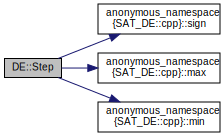
\includegraphics[width=296pt]{classDE_ac45486f7c7bf422c6bd024aba501a2a2_cgraph}
\end{center}
\end{figure}




Here is the caller graph for this function\-:\nopagebreak
\begin{figure}[H]
\begin{center}
\leavevmode
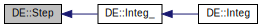
\includegraphics[width=334pt]{classDE_ac45486f7c7bf422c6bd024aba501a2a2_icgraph}
\end{center}
\end{figure}




\subsection{Member Data Documentation}
\hypertarget{classDE_a9337b177c5adfeda779ceecd6b56b370}{\index{D\-E@{D\-E}!abserr@{abserr}}
\index{abserr@{abserr}!DE@{D\-E}}
\subsubsection[{abserr}]{\setlength{\rightskip}{0pt plus 5cm}double D\-E\-::abserr}}\label{classDE_a9337b177c5adfeda779ceecd6b56b370}


Definition at line 133 of file S\-A\-T\-\_\-\-D\-E.\-h.

\hypertarget{classDE_ad0bf62cec063071d0773fde29d976c0e}{\index{D\-E@{D\-E}!alpha@{alpha}}
\index{alpha@{alpha}!DE@{D\-E}}
\subsubsection[{alpha}]{\setlength{\rightskip}{0pt plus 5cm}double D\-E\-::alpha\mbox{[}13\mbox{]}\hspace{0.3cm}{\ttfamily [private]}}}\label{classDE_ad0bf62cec063071d0773fde29d976c0e}


Definition at line 181 of file S\-A\-T\-\_\-\-D\-E.\-h.

\hypertarget{classDE_a6db4afe37f9ebf0dce0532415c40de32}{\index{D\-E@{D\-E}!beta@{beta}}
\index{beta@{beta}!DE@{D\-E}}
\subsubsection[{beta}]{\setlength{\rightskip}{0pt plus 5cm}double D\-E\-::beta\mbox{[}13\mbox{]}\hspace{0.3cm}{\ttfamily [private]}}}\label{classDE_a6db4afe37f9ebf0dce0532415c40de32}


Definition at line 181 of file S\-A\-T\-\_\-\-D\-E.\-h.

\hypertarget{classDE_a5fe0648747453fc746c8bee223d58633}{\index{D\-E@{D\-E}!delsgn@{delsgn}}
\index{delsgn@{delsgn}!DE@{D\-E}}
\subsubsection[{delsgn}]{\setlength{\rightskip}{0pt plus 5cm}double D\-E\-::delsgn\hspace{0.3cm}{\ttfamily [private]}}}\label{classDE_a5fe0648747453fc746c8bee223d58633}


Definition at line 183 of file S\-A\-T\-\_\-\-D\-E.\-h.

\hypertarget{classDE_afa7fefa0ba10ee635a618b3a4a5a39dc}{\index{D\-E@{D\-E}!f@{f}}
\index{f@{f}!DE@{D\-E}}
\subsubsection[{f}]{\setlength{\rightskip}{0pt plus 5cm}{\bf D\-Efunct} D\-E\-::f\hspace{0.3cm}{\ttfamily [private]}}}\label{classDE_afa7fefa0ba10ee635a618b3a4a5a39dc}


Definition at line 176 of file S\-A\-T\-\_\-\-D\-E.\-h.

\hypertarget{classDE_aa5b66f7465475382f7f2d757fd9cf979}{\index{D\-E@{D\-E}!g@{g}}
\index{g@{g}!DE@{D\-E}}
\subsubsection[{g}]{\setlength{\rightskip}{0pt plus 5cm}double D\-E\-::g\mbox{[}14\mbox{]}\hspace{0.3cm}{\ttfamily [private]}}}\label{classDE_aa5b66f7465475382f7f2d757fd9cf979}


Definition at line 182 of file S\-A\-T\-\_\-\-D\-E.\-h.

\hypertarget{classDE_adcd1d27f91dc1de8c4e2e8572878f92f}{\index{D\-E@{D\-E}!h@{h}}
\index{h@{h}!DE@{D\-E}}
\subsubsection[{h}]{\setlength{\rightskip}{0pt plus 5cm}double D\-E\-::h\hspace{0.3cm}{\ttfamily [private]}}}\label{classDE_adcd1d27f91dc1de8c4e2e8572878f92f}


Definition at line 183 of file S\-A\-T\-\_\-\-D\-E.\-h.

\hypertarget{classDE_a8aba1f4cf3cb574060e0772052b6772e}{\index{D\-E@{D\-E}!hold@{hold}}
\index{hold@{hold}!DE@{D\-E}}
\subsubsection[{hold}]{\setlength{\rightskip}{0pt plus 5cm}double D\-E\-::hold\hspace{0.3cm}{\ttfamily [private]}}}\label{classDE_a8aba1f4cf3cb574060e0772052b6772e}


Definition at line 183 of file S\-A\-T\-\_\-\-D\-E.\-h.

\hypertarget{classDE_a992636687bf14328677c450008855770}{\index{D\-E@{D\-E}!init@{init}}
\index{init@{init}!DE@{D\-E}}
\subsubsection[{init}]{\setlength{\rightskip}{0pt plus 5cm}bool D\-E\-::init\hspace{0.3cm}{\ttfamily [private]}}}\label{classDE_a992636687bf14328677c450008855770}


Definition at line 186 of file S\-A\-T\-\_\-\-D\-E.\-h.

\hypertarget{classDE_a583b51553ddbe1eb995e76d42b2e13ec}{\index{D\-E@{D\-E}!k@{k}}
\index{k@{k}!DE@{D\-E}}
\subsubsection[{k}]{\setlength{\rightskip}{0pt plus 5cm}int D\-E\-::k\hspace{0.3cm}{\ttfamily [private]}}}\label{classDE_a583b51553ddbe1eb995e76d42b2e13ec}


Definition at line 184 of file S\-A\-T\-\_\-\-D\-E.\-h.

\hypertarget{classDE_aaa4409f0e1999d15aa33da045dcf464d}{\index{D\-E@{D\-E}!kold@{kold}}
\index{kold@{kold}!DE@{D\-E}}
\subsubsection[{kold}]{\setlength{\rightskip}{0pt plus 5cm}int D\-E\-::kold\hspace{0.3cm}{\ttfamily [private]}}}\label{classDE_aaa4409f0e1999d15aa33da045dcf464d}


Definition at line 184 of file S\-A\-T\-\_\-\-D\-E.\-h.

\hypertarget{classDE_ae74a30c7f5448d96d8460b4fde65f849}{\index{D\-E@{D\-E}!n\-\_\-eqn@{n\-\_\-eqn}}
\index{n\-\_\-eqn@{n\-\_\-eqn}!DE@{D\-E}}
\subsubsection[{n\-\_\-eqn}]{\setlength{\rightskip}{0pt plus 5cm}int D\-E\-::n\-\_\-eqn\hspace{0.3cm}{\ttfamily [private]}}}\label{classDE_ae74a30c7f5448d96d8460b4fde65f849}


Definition at line 177 of file S\-A\-T\-\_\-\-D\-E.\-h.

\hypertarget{classDE_ab7d114c0f93009e0deddea4375764e52}{\index{D\-E@{D\-E}!nornd@{nornd}}
\index{nornd@{nornd}!DE@{D\-E}}
\subsubsection[{nornd}]{\setlength{\rightskip}{0pt plus 5cm}bool D\-E\-::nornd\hspace{0.3cm}{\ttfamily [private]}}}\label{classDE_ab7d114c0f93009e0deddea4375764e52}


Definition at line 185 of file S\-A\-T\-\_\-\-D\-E.\-h.

\hypertarget{classDE_a4d82322b4499d5f8e27f2e19675fcfa6}{\index{D\-E@{D\-E}!ns@{ns}}
\index{ns@{ns}!DE@{D\-E}}
\subsubsection[{ns}]{\setlength{\rightskip}{0pt plus 5cm}int D\-E\-::ns\hspace{0.3cm}{\ttfamily [private]}}}\label{classDE_a4d82322b4499d5f8e27f2e19675fcfa6}


Definition at line 184 of file S\-A\-T\-\_\-\-D\-E.\-h.

\hypertarget{classDE_a210930a504af06e95856cb71411b2a6b}{\index{D\-E@{D\-E}!Old\-Permit@{Old\-Permit}}
\index{Old\-Permit@{Old\-Permit}!DE@{D\-E}}
\subsubsection[{Old\-Permit}]{\setlength{\rightskip}{0pt plus 5cm}bool D\-E\-::\-Old\-Permit\hspace{0.3cm}{\ttfamily [private]}}}\label{classDE_a210930a504af06e95856cb71411b2a6b}


Definition at line 185 of file S\-A\-T\-\_\-\-D\-E.\-h.

\hypertarget{classDE_af16ce45fb590ddb2ae5225b5cfc95f87}{\index{D\-E@{D\-E}!p@{p}}
\index{p@{p}!DE@{D\-E}}
\subsubsection[{p}]{\setlength{\rightskip}{0pt plus 5cm}{\bf Vector} D\-E\-::p\hspace{0.3cm}{\ttfamily [private]}}}\label{classDE_af16ce45fb590ddb2ae5225b5cfc95f87}


Definition at line 179 of file S\-A\-T\-\_\-\-D\-E.\-h.

\hypertarget{classDE_ab8fad10a55cec3f9755444ae5ee38903}{\index{D\-E@{D\-E}!p\-Aux@{p\-Aux}}
\index{p\-Aux@{p\-Aux}!DE@{D\-E}}
\subsubsection[{p\-Aux}]{\setlength{\rightskip}{0pt plus 5cm}void$\ast$ D\-E\-::p\-Aux\hspace{0.3cm}{\ttfamily [private]}}}\label{classDE_ab8fad10a55cec3f9755444ae5ee38903}


Definition at line 178 of file S\-A\-T\-\_\-\-D\-E.\-h.

\hypertarget{classDE_ab4adac8a112f4c5b5600986b418e5129}{\index{D\-E@{D\-E}!Permit\-T\-O\-U\-T@{Permit\-T\-O\-U\-T}}
\index{Permit\-T\-O\-U\-T@{Permit\-T\-O\-U\-T}!DE@{D\-E}}
\subsubsection[{Permit\-T\-O\-U\-T}]{\setlength{\rightskip}{0pt plus 5cm}bool D\-E\-::\-Permit\-T\-O\-U\-T}}\label{classDE_ab4adac8a112f4c5b5600986b418e5129}


Definition at line 135 of file S\-A\-T\-\_\-\-D\-E.\-h.

\hypertarget{classDE_ab9a2adeb8253f3901c1cb39387e35fba}{\index{D\-E@{D\-E}!phase1@{phase1}}
\index{phase1@{phase1}!DE@{D\-E}}
\subsubsection[{phase1}]{\setlength{\rightskip}{0pt plus 5cm}bool D\-E\-::phase1\hspace{0.3cm}{\ttfamily [private]}}}\label{classDE_ab9a2adeb8253f3901c1cb39387e35fba}


Definition at line 185 of file S\-A\-T\-\_\-\-D\-E.\-h.

\hypertarget{classDE_a79eb189fb7f3320d735b90ca3332311e}{\index{D\-E@{D\-E}!phi@{phi}}
\index{phi@{phi}!DE@{D\-E}}
\subsubsection[{phi}]{\setlength{\rightskip}{0pt plus 5cm}{\bf Matrix} D\-E\-::phi\hspace{0.3cm}{\ttfamily [private]}}}\label{classDE_a79eb189fb7f3320d735b90ca3332311e}


Definition at line 180 of file S\-A\-T\-\_\-\-D\-E.\-h.

\hypertarget{classDE_a7ef55ab5c646e5f540adcfa6ed392b56}{\index{D\-E@{D\-E}!psi@{psi}}
\index{psi@{psi}!DE@{D\-E}}
\subsubsection[{psi}]{\setlength{\rightskip}{0pt plus 5cm}double D\-E\-::psi\mbox{[}13\mbox{]}\hspace{0.3cm}{\ttfamily [private]}}}\label{classDE_a7ef55ab5c646e5f540adcfa6ed392b56}


Definition at line 181 of file S\-A\-T\-\_\-\-D\-E.\-h.

\hypertarget{classDE_a877edbd8bd4ba297b5602786b552059f}{\index{D\-E@{D\-E}!relerr@{relerr}}
\index{relerr@{relerr}!DE@{D\-E}}
\subsubsection[{relerr}]{\setlength{\rightskip}{0pt plus 5cm}double D\-E\-::relerr}}\label{classDE_a877edbd8bd4ba297b5602786b552059f}


Definition at line 132 of file S\-A\-T\-\_\-\-D\-E.\-h.

\hypertarget{classDE_a2ec1db657ea1d2ba57e0221ca0cb3eef}{\index{D\-E@{D\-E}!sig@{sig}}
\index{sig@{sig}!DE@{D\-E}}
\subsubsection[{sig}]{\setlength{\rightskip}{0pt plus 5cm}double D\-E\-::sig\mbox{[}14\mbox{]}\hspace{0.3cm}{\ttfamily [private]}}}\label{classDE_a2ec1db657ea1d2ba57e0221ca0cb3eef}


Definition at line 182 of file S\-A\-T\-\_\-\-D\-E.\-h.

\hypertarget{classDE_a3c9b03623043eee0c38ecefecf301320}{\index{D\-E@{D\-E}!start@{start}}
\index{start@{start}!DE@{D\-E}}
\subsubsection[{start}]{\setlength{\rightskip}{0pt plus 5cm}bool D\-E\-::start\hspace{0.3cm}{\ttfamily [private]}}}\label{classDE_a3c9b03623043eee0c38ecefecf301320}


Definition at line 185 of file S\-A\-T\-\_\-\-D\-E.\-h.

\hypertarget{classDE_a1d99a54650b09e8192bf89537f66bed2}{\index{D\-E@{D\-E}!State@{State}}
\index{State@{State}!DE@{D\-E}}
\subsubsection[{State}]{\setlength{\rightskip}{0pt plus 5cm}{\bf D\-E\-\_\-\-S\-T\-A\-T\-E} D\-E\-::\-State}}\label{classDE_a1d99a54650b09e8192bf89537f66bed2}


Definition at line 134 of file S\-A\-T\-\_\-\-D\-E.\-h.

\hypertarget{classDE_a56ee5af65170db9321a5508c207cd173}{\index{D\-E@{D\-E}!t@{t}}
\index{t@{t}!DE@{D\-E}}
\subsubsection[{t}]{\setlength{\rightskip}{0pt plus 5cm}double D\-E\-::t}}\label{classDE_a56ee5af65170db9321a5508c207cd173}


Definition at line 137 of file S\-A\-T\-\_\-\-D\-E.\-h.

\hypertarget{classDE_a710c5e85925a2ce84f8d789c1b4cb99b}{\index{D\-E@{D\-E}!told@{told}}
\index{told@{told}!DE@{D\-E}}
\subsubsection[{told}]{\setlength{\rightskip}{0pt plus 5cm}double D\-E\-::told\hspace{0.3cm}{\ttfamily [private]}}}\label{classDE_a710c5e85925a2ce84f8d789c1b4cb99b}


Definition at line 183 of file S\-A\-T\-\_\-\-D\-E.\-h.

\hypertarget{classDE_af4b92bb3bf10322b581dbbcf778ef5d5}{\index{D\-E@{D\-E}!v@{v}}
\index{v@{v}!DE@{D\-E}}
\subsubsection[{v}]{\setlength{\rightskip}{0pt plus 5cm}double D\-E\-::v\mbox{[}13\mbox{]}\hspace{0.3cm}{\ttfamily [private]}}}\label{classDE_af4b92bb3bf10322b581dbbcf778ef5d5}


Definition at line 181 of file S\-A\-T\-\_\-\-D\-E.\-h.

\hypertarget{classDE_a4cd9f3da02faec86f2926ce373a4e7c9}{\index{D\-E@{D\-E}!w@{w}}
\index{w@{w}!DE@{D\-E}}
\subsubsection[{w}]{\setlength{\rightskip}{0pt plus 5cm}double D\-E\-::w\mbox{[}13\mbox{]}\hspace{0.3cm}{\ttfamily [private]}}}\label{classDE_a4cd9f3da02faec86f2926ce373a4e7c9}


Definition at line 181 of file S\-A\-T\-\_\-\-D\-E.\-h.

\hypertarget{classDE_adc470cb3c810cd47c8603003f10d4cac}{\index{D\-E@{D\-E}!wt@{wt}}
\index{wt@{wt}!DE@{D\-E}}
\subsubsection[{wt}]{\setlength{\rightskip}{0pt plus 5cm}{\bf Vector} D\-E\-::wt\hspace{0.3cm}{\ttfamily [private]}}}\label{classDE_adc470cb3c810cd47c8603003f10d4cac}


Definition at line 179 of file S\-A\-T\-\_\-\-D\-E.\-h.

\hypertarget{classDE_a53686f8f7ab89225ba80835e910168fa}{\index{D\-E@{D\-E}!x@{x}}
\index{x@{x}!DE@{D\-E}}
\subsubsection[{x}]{\setlength{\rightskip}{0pt plus 5cm}double D\-E\-::x\hspace{0.3cm}{\ttfamily [private]}}}\label{classDE_a53686f8f7ab89225ba80835e910168fa}


Definition at line 183 of file S\-A\-T\-\_\-\-D\-E.\-h.

\hypertarget{classDE_acff3aaf84faff7827daf981587ef5b03}{\index{D\-E@{D\-E}!yp@{yp}}
\index{yp@{yp}!DE@{D\-E}}
\subsubsection[{yp}]{\setlength{\rightskip}{0pt plus 5cm}{\bf Vector} D\-E\-::yp\hspace{0.3cm}{\ttfamily [private]}}}\label{classDE_acff3aaf84faff7827daf981587ef5b03}


Definition at line 179 of file S\-A\-T\-\_\-\-D\-E.\-h.

\hypertarget{classDE_a985edfb71c582371040affbd4230a36a}{\index{D\-E@{D\-E}!ypout@{ypout}}
\index{ypout@{ypout}!DE@{D\-E}}
\subsubsection[{ypout}]{\setlength{\rightskip}{0pt plus 5cm}{\bf Vector} D\-E\-::ypout\hspace{0.3cm}{\ttfamily [private]}}}\label{classDE_a985edfb71c582371040affbd4230a36a}


Definition at line 179 of file S\-A\-T\-\_\-\-D\-E.\-h.

\hypertarget{classDE_ab501e078b2408ca63ee44c1c4d59de86}{\index{D\-E@{D\-E}!yy@{yy}}
\index{yy@{yy}!DE@{D\-E}}
\subsubsection[{yy}]{\setlength{\rightskip}{0pt plus 5cm}{\bf Vector} D\-E\-::yy\hspace{0.3cm}{\ttfamily [private]}}}\label{classDE_ab501e078b2408ca63ee44c1c4d59de86}


Definition at line 179 of file S\-A\-T\-\_\-\-D\-E.\-h.



The documentation for this class was generated from the following files\-:\begin{DoxyCompactItemize}
\item 
\hyperlink{SAT__DE_8h}{S\-A\-T\-\_\-\-D\-E.\-h}\item 
\hyperlink{SAT__DE_8cpp}{S\-A\-T\-\_\-\-D\-E.\-cpp}\end{DoxyCompactItemize}

\hypertarget{classEKF}{\section{E\-K\-F Class Reference}
\label{classEKF}\index{E\-K\-F@{E\-K\-F}}
}


{\ttfamily \#include $<$S\-A\-T\-\_\-\-Filter.\-h$>$}



Collaboration diagram for E\-K\-F\-:\nopagebreak
\begin{figure}[H]
\begin{center}
\leavevmode
\includegraphics[width=187pt]{classEKF__coll__graph}
\end{center}
\end{figure}
\subsection*{Public Member Functions}
\begin{DoxyCompactItemize}
\item 
\hyperlink{classEKF_ac3ea8221d535e025dfd9e330d1bc3e72}{E\-K\-F} (int n\-\_\-)
\item 
void \hyperlink{classEKF_acf949c77d116256b94cb4f56b874de4e}{Init} (double t\-\_\-, \hyperlink{classVector}{Vector} x\-\_\-, \hyperlink{classMatrix}{Matrix} P\-\_\-)
\item 
void \hyperlink{classEKF_aca56e0778d22bf7899716cdac757b909}{Init} (double t\-\_\-, \hyperlink{classVector}{Vector} x\-\_\-, \hyperlink{classVector}{Vector} sigma)
\item 
void \hyperlink{classEKF_a581eb4063feb02eeff09dabeaf07e994}{Time\-Update} (double t\-\_\-, const \hyperlink{classVector}{Vector} \&x\-\_\-, const \hyperlink{classMatrix}{Matrix} \&\hyperlink{GEODA_8cpp_ad363d83dfb0be87465bd76a2e5e0ff6b}{Phi})
\item 
void \hyperlink{classEKF_ac9e0e9b6f423ad75fc71eae01d785930}{Time\-Update} (double t\-\_\-, const \hyperlink{classVector}{Vector} \&x\-\_\-, const \hyperlink{classMatrix}{Matrix} \&\hyperlink{GEODA_8cpp_ad363d83dfb0be87465bd76a2e5e0ff6b}{Phi}, const \hyperlink{classMatrix}{Matrix} \&Qdt)
\item 
void \hyperlink{classEKF_a2384ab018c26960ee808a9a1ae66d319}{Meas\-Update} (double z, double g, double sigma, const \hyperlink{classVector}{Vector} \&G)
\item 
void \hyperlink{classEKF_a080c81bbef29da2b57caa52775f76602}{Meas\-Update} (const \hyperlink{classVector}{Vector} \&z, const \hyperlink{classVector}{Vector} \&g, const \hyperlink{classVector}{Vector} \&s, const \hyperlink{classMatrix}{Matrix} \&G)
\item 
void \hyperlink{classEKF_afe7d00a0c74d8c0bfa98574233445a0a}{Meas\-Update} (const \hyperlink{classVector}{Vector} \&z, const \hyperlink{classVector}{Vector} \&g, const \hyperlink{classMatrix}{Matrix} \&Inv\-\_\-\-W, const \hyperlink{classMatrix}{Matrix} \&G)
\item 
double \hyperlink{classEKF_aca97d9e3ba20ff1ac5dbf1c4a913c989}{Time} ()
\item 
\hyperlink{classVector}{Vector} \hyperlink{classEKF_accc2ee72c5f8727727fafffe6cf0c10a}{State} ()
\item 
\hyperlink{classMatrix}{Matrix} \hyperlink{classEKF_a796ecb81da82ddbaa790cea3dde7435f}{Cov} ()
\item 
\hyperlink{classVector}{Vector} \hyperlink{classEKF_ada67f575947bfc34de84584724b1a16e}{Std\-Dev} ()
\end{DoxyCompactItemize}
\subsection*{Private Attributes}
\begin{DoxyCompactItemize}
\item 
int \hyperlink{classEKF_ad6067337de951c9e7d92d03e02c85ec3}{n}
\item 
double \hyperlink{classEKF_aeff02227c21d484b916191b9af470e31}{t}
\item 
\hyperlink{classVector}{Vector} \hyperlink{classEKF_af4e80565150dfd65e4bc508fe3b1d674}{x}
\item 
\hyperlink{classMatrix}{Matrix} \hyperlink{classEKF_a2f89c66ecddb3b26a3797d5dc48fb2af}{P}
\end{DoxyCompactItemize}


\subsection{Detailed Description}


Definition at line 118 of file S\-A\-T\-\_\-\-Filter.\-h.



\subsection{Constructor \& Destructor Documentation}
\hypertarget{classEKF_ac3ea8221d535e025dfd9e330d1bc3e72}{\index{E\-K\-F@{E\-K\-F}!E\-K\-F@{E\-K\-F}}
\index{E\-K\-F@{E\-K\-F}!EKF@{E\-K\-F}}
\subsubsection[{E\-K\-F}]{\setlength{\rightskip}{0pt plus 5cm}E\-K\-F\-::\-E\-K\-F (
\begin{DoxyParamCaption}
\item[{int}]{n\-\_\-}
\end{DoxyParamCaption}
)}}\label{classEKF_ac3ea8221d535e025dfd9e330d1bc3e72}


Definition at line 332 of file S\-A\-T\-\_\-\-Filter.\-cpp.



\subsection{Member Function Documentation}
\hypertarget{classEKF_a796ecb81da82ddbaa790cea3dde7435f}{\index{E\-K\-F@{E\-K\-F}!Cov@{Cov}}
\index{Cov@{Cov}!EKF@{E\-K\-F}}
\subsubsection[{Cov}]{\setlength{\rightskip}{0pt plus 5cm}{\bf Matrix} E\-K\-F\-::\-Cov (
\begin{DoxyParamCaption}
{}
\end{DoxyParamCaption}
)}}\label{classEKF_a796ecb81da82ddbaa790cea3dde7435f}


Definition at line 366 of file S\-A\-T\-\_\-\-Filter.\-cpp.



Here is the caller graph for this function\-:\nopagebreak
\begin{figure}[H]
\begin{center}
\leavevmode
\includegraphics[width=214pt]{classEKF_a796ecb81da82ddbaa790cea3dde7435f_icgraph}
\end{center}
\end{figure}


\hypertarget{classEKF_acf949c77d116256b94cb4f56b874de4e}{\index{E\-K\-F@{E\-K\-F}!Init@{Init}}
\index{Init@{Init}!EKF@{E\-K\-F}}
\subsubsection[{Init}]{\setlength{\rightskip}{0pt plus 5cm}void E\-K\-F\-::\-Init (
\begin{DoxyParamCaption}
\item[{double}]{t\-\_\-, }
\item[{{\bf Vector}}]{x\-\_\-, }
\item[{{\bf Matrix}}]{P\-\_\-}
\end{DoxyParamCaption}
)}}\label{classEKF_acf949c77d116256b94cb4f56b874de4e}


Definition at line 345 of file S\-A\-T\-\_\-\-Filter.\-cpp.



Here is the caller graph for this function\-:\nopagebreak
\begin{figure}[H]
\begin{center}
\leavevmode
\includegraphics[width=210pt]{classEKF_acf949c77d116256b94cb4f56b874de4e_icgraph}
\end{center}
\end{figure}


\hypertarget{classEKF_aca56e0778d22bf7899716cdac757b909}{\index{E\-K\-F@{E\-K\-F}!Init@{Init}}
\index{Init@{Init}!EKF@{E\-K\-F}}
\subsubsection[{Init}]{\setlength{\rightskip}{0pt plus 5cm}void E\-K\-F\-::\-Init (
\begin{DoxyParamCaption}
\item[{double}]{t\-\_\-, }
\item[{{\bf Vector}}]{x\-\_\-, }
\item[{{\bf Vector}}]{sigma}
\end{DoxyParamCaption}
)}}\label{classEKF_aca56e0778d22bf7899716cdac757b909}


Definition at line 350 of file S\-A\-T\-\_\-\-Filter.\-cpp.

\hypertarget{classEKF_a2384ab018c26960ee808a9a1ae66d319}{\index{E\-K\-F@{E\-K\-F}!Meas\-Update@{Meas\-Update}}
\index{Meas\-Update@{Meas\-Update}!EKF@{E\-K\-F}}
\subsubsection[{Meas\-Update}]{\setlength{\rightskip}{0pt plus 5cm}void E\-K\-F\-::\-Meas\-Update (
\begin{DoxyParamCaption}
\item[{double}]{z, }
\item[{double}]{g, }
\item[{double}]{sigma, }
\item[{const {\bf Vector} \&}]{G}
\end{DoxyParamCaption}
)}}\label{classEKF_a2384ab018c26960ee808a9a1ae66d319}


Definition at line 399 of file S\-A\-T\-\_\-\-Filter.\-cpp.



Here is the call graph for this function\-:\nopagebreak
\begin{figure}[H]
\begin{center}
\leavevmode
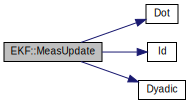
\includegraphics[width=262pt]{classEKF_a2384ab018c26960ee808a9a1ae66d319_cgraph}
\end{center}
\end{figure}




Here is the caller graph for this function\-:\nopagebreak
\begin{figure}[H]
\begin{center}
\leavevmode
\includegraphics[width=252pt]{classEKF_a2384ab018c26960ee808a9a1ae66d319_icgraph}
\end{center}
\end{figure}


\hypertarget{classEKF_a080c81bbef29da2b57caa52775f76602}{\index{E\-K\-F@{E\-K\-F}!Meas\-Update@{Meas\-Update}}
\index{Meas\-Update@{Meas\-Update}!EKF@{E\-K\-F}}
\subsubsection[{Meas\-Update}]{\setlength{\rightskip}{0pt plus 5cm}void E\-K\-F\-::\-Meas\-Update (
\begin{DoxyParamCaption}
\item[{const {\bf Vector} \&}]{z, }
\item[{const {\bf Vector} \&}]{g, }
\item[{const {\bf Vector} \&}]{s, }
\item[{const {\bf Matrix} \&}]{G}
\end{DoxyParamCaption}
)}}\label{classEKF_a080c81bbef29da2b57caa52775f76602}


Definition at line 422 of file S\-A\-T\-\_\-\-Filter.\-cpp.



Here is the call graph for this function\-:\nopagebreak
\begin{figure}[H]
\begin{center}
\leavevmode
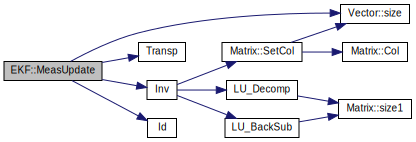
\includegraphics[width=350pt]{classEKF_a080c81bbef29da2b57caa52775f76602_cgraph}
\end{center}
\end{figure}


\hypertarget{classEKF_afe7d00a0c74d8c0bfa98574233445a0a}{\index{E\-K\-F@{E\-K\-F}!Meas\-Update@{Meas\-Update}}
\index{Meas\-Update@{Meas\-Update}!EKF@{E\-K\-F}}
\subsubsection[{Meas\-Update}]{\setlength{\rightskip}{0pt plus 5cm}void E\-K\-F\-::\-Meas\-Update (
\begin{DoxyParamCaption}
\item[{const {\bf Vector} \&}]{z, }
\item[{const {\bf Vector} \&}]{g, }
\item[{const {\bf Matrix} \&}]{Inv\-\_\-\-W, }
\item[{const {\bf Matrix} \&}]{G}
\end{DoxyParamCaption}
)}}\label{classEKF_afe7d00a0c74d8c0bfa98574233445a0a}


Definition at line 456 of file S\-A\-T\-\_\-\-Filter.\-cpp.



Here is the call graph for this function\-:\nopagebreak
\begin{figure}[H]
\begin{center}
\leavevmode
\includegraphics[width=350pt]{classEKF_afe7d00a0c74d8c0bfa98574233445a0a_cgraph}
\end{center}
\end{figure}


\hypertarget{classEKF_accc2ee72c5f8727727fafffe6cf0c10a}{\index{E\-K\-F@{E\-K\-F}!State@{State}}
\index{State@{State}!EKF@{E\-K\-F}}
\subsubsection[{State}]{\setlength{\rightskip}{0pt plus 5cm}{\bf Vector} E\-K\-F\-::\-State (
\begin{DoxyParamCaption}
{}
\end{DoxyParamCaption}
)}}\label{classEKF_accc2ee72c5f8727727fafffe6cf0c10a}


Definition at line 364 of file S\-A\-T\-\_\-\-Filter.\-cpp.



Here is the caller graph for this function\-:\nopagebreak
\begin{figure}[H]
\begin{center}
\leavevmode
\includegraphics[width=220pt]{classEKF_accc2ee72c5f8727727fafffe6cf0c10a_icgraph}
\end{center}
\end{figure}


\hypertarget{classEKF_ada67f575947bfc34de84584724b1a16e}{\index{E\-K\-F@{E\-K\-F}!Std\-Dev@{Std\-Dev}}
\index{Std\-Dev@{Std\-Dev}!EKF@{E\-K\-F}}
\subsubsection[{Std\-Dev}]{\setlength{\rightskip}{0pt plus 5cm}{\bf Vector} E\-K\-F\-::\-Std\-Dev (
\begin{DoxyParamCaption}
{}
\end{DoxyParamCaption}
)}}\label{classEKF_ada67f575947bfc34de84584724b1a16e}


Definition at line 368 of file S\-A\-T\-\_\-\-Filter.\-cpp.



Here is the caller graph for this function\-:\nopagebreak
\begin{figure}[H]
\begin{center}
\leavevmode
\includegraphics[width=230pt]{classEKF_ada67f575947bfc34de84584724b1a16e_icgraph}
\end{center}
\end{figure}


\hypertarget{classEKF_aca97d9e3ba20ff1ac5dbf1c4a913c989}{\index{E\-K\-F@{E\-K\-F}!Time@{Time}}
\index{Time@{Time}!EKF@{E\-K\-F}}
\subsubsection[{Time}]{\setlength{\rightskip}{0pt plus 5cm}double E\-K\-F\-::\-Time (
\begin{DoxyParamCaption}
{}
\end{DoxyParamCaption}
)}}\label{classEKF_aca97d9e3ba20ff1ac5dbf1c4a913c989}


Definition at line 362 of file S\-A\-T\-\_\-\-Filter.\-cpp.



Here is the caller graph for this function\-:\nopagebreak
\begin{figure}[H]
\begin{center}
\leavevmode
\includegraphics[width=218pt]{classEKF_aca97d9e3ba20ff1ac5dbf1c4a913c989_icgraph}
\end{center}
\end{figure}


\hypertarget{classEKF_a581eb4063feb02eeff09dabeaf07e994}{\index{E\-K\-F@{E\-K\-F}!Time\-Update@{Time\-Update}}
\index{Time\-Update@{Time\-Update}!EKF@{E\-K\-F}}
\subsubsection[{Time\-Update}]{\setlength{\rightskip}{0pt plus 5cm}void E\-K\-F\-::\-Time\-Update (
\begin{DoxyParamCaption}
\item[{double}]{t\-\_\-, }
\item[{const {\bf Vector} \&}]{x\-\_\-, }
\item[{const {\bf Matrix} \&}]{Phi}
\end{DoxyParamCaption}
)}}\label{classEKF_a581eb4063feb02eeff09dabeaf07e994}


Definition at line 378 of file S\-A\-T\-\_\-\-Filter.\-cpp.



Here is the call graph for this function\-:\nopagebreak
\begin{figure}[H]
\begin{center}
\leavevmode
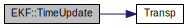
\includegraphics[width=260pt]{classEKF_a581eb4063feb02eeff09dabeaf07e994_cgraph}
\end{center}
\end{figure}




Here is the caller graph for this function\-:\nopagebreak
\begin{figure}[H]
\begin{center}
\leavevmode
\includegraphics[width=250pt]{classEKF_a581eb4063feb02eeff09dabeaf07e994_icgraph}
\end{center}
\end{figure}


\hypertarget{classEKF_ac9e0e9b6f423ad75fc71eae01d785930}{\index{E\-K\-F@{E\-K\-F}!Time\-Update@{Time\-Update}}
\index{Time\-Update@{Time\-Update}!EKF@{E\-K\-F}}
\subsubsection[{Time\-Update}]{\setlength{\rightskip}{0pt plus 5cm}void E\-K\-F\-::\-Time\-Update (
\begin{DoxyParamCaption}
\item[{double}]{t\-\_\-, }
\item[{const {\bf Vector} \&}]{x\-\_\-, }
\item[{const {\bf Matrix} \&}]{Phi, }
\item[{const {\bf Matrix} \&}]{Qdt}
\end{DoxyParamCaption}
)}}\label{classEKF_ac9e0e9b6f423ad75fc71eae01d785930}


Definition at line 385 of file S\-A\-T\-\_\-\-Filter.\-cpp.



Here is the call graph for this function\-:\nopagebreak
\begin{figure}[H]
\begin{center}
\leavevmode
\includegraphics[width=260pt]{classEKF_ac9e0e9b6f423ad75fc71eae01d785930_cgraph}
\end{center}
\end{figure}




\subsection{Member Data Documentation}
\hypertarget{classEKF_ad6067337de951c9e7d92d03e02c85ec3}{\index{E\-K\-F@{E\-K\-F}!n@{n}}
\index{n@{n}!EKF@{E\-K\-F}}
\subsubsection[{n}]{\setlength{\rightskip}{0pt plus 5cm}int E\-K\-F\-::n\hspace{0.3cm}{\ttfamily [private]}}}\label{classEKF_ad6067337de951c9e7d92d03e02c85ec3}


Definition at line 166 of file S\-A\-T\-\_\-\-Filter.\-h.

\hypertarget{classEKF_a2f89c66ecddb3b26a3797d5dc48fb2af}{\index{E\-K\-F@{E\-K\-F}!P@{P}}
\index{P@{P}!EKF@{E\-K\-F}}
\subsubsection[{P}]{\setlength{\rightskip}{0pt plus 5cm}{\bf Matrix} E\-K\-F\-::\-P\hspace{0.3cm}{\ttfamily [private]}}}\label{classEKF_a2f89c66ecddb3b26a3797d5dc48fb2af}


Definition at line 169 of file S\-A\-T\-\_\-\-Filter.\-h.

\hypertarget{classEKF_aeff02227c21d484b916191b9af470e31}{\index{E\-K\-F@{E\-K\-F}!t@{t}}
\index{t@{t}!EKF@{E\-K\-F}}
\subsubsection[{t}]{\setlength{\rightskip}{0pt plus 5cm}double E\-K\-F\-::t\hspace{0.3cm}{\ttfamily [private]}}}\label{classEKF_aeff02227c21d484b916191b9af470e31}


Definition at line 167 of file S\-A\-T\-\_\-\-Filter.\-h.

\hypertarget{classEKF_af4e80565150dfd65e4bc508fe3b1d674}{\index{E\-K\-F@{E\-K\-F}!x@{x}}
\index{x@{x}!EKF@{E\-K\-F}}
\subsubsection[{x}]{\setlength{\rightskip}{0pt plus 5cm}{\bf Vector} E\-K\-F\-::x\hspace{0.3cm}{\ttfamily [private]}}}\label{classEKF_af4e80565150dfd65e4bc508fe3b1d674}


Definition at line 168 of file S\-A\-T\-\_\-\-Filter.\-h.



The documentation for this class was generated from the following files\-:\begin{DoxyCompactItemize}
\item 
\hyperlink{SAT__Filter_8h}{S\-A\-T\-\_\-\-Filter.\-h}\item 
\hyperlink{SAT__Filter_8cpp}{S\-A\-T\-\_\-\-Filter.\-cpp}\end{DoxyCompactItemize}

\hypertarget{classGeodetic}{\section{Geodetic Class Reference}
\label{classGeodetic}\index{Geodetic@{Geodetic}}
}


{\ttfamily \#include $<$S\-A\-T\-\_\-\-Ref\-Sys.\-h$>$}

\subsection*{Public Member Functions}
\begin{DoxyCompactItemize}
\item 
\hyperlink{classGeodetic_a3f673f6471171da70ef7fb27b90a0737}{Geodetic} ()
\item 
\hyperlink{classGeodetic_ae97afd6fa6138fbe24496f1345ac27fc}{Geodetic} (double lambda, double phi, double alt)
\item 
\hyperlink{classGeodetic_ad813b9417dac1cee7ea962c36b82bb9c}{Geodetic} (\hyperlink{classVector}{Vector} r, double R\-\_\-equ=\hyperlink{SAT__Const_8h_a0232432b945403a113096bb07fa21c09}{R\-\_\-\-Earth}, double f=\hyperlink{SAT__Const_8h_ae88715365ab0f6239981068fc94297c1}{f\-\_\-\-Earth})
\item 
\hyperlink{classVector}{Vector} \hyperlink{classGeodetic_a7c02e1089d2fc2eebd46a20252e78130}{Position} (double R\-\_\-equ=\hyperlink{SAT__Const_8h_a0232432b945403a113096bb07fa21c09}{R\-\_\-\-Earth}, double f=\hyperlink{SAT__Const_8h_ae88715365ab0f6239981068fc94297c1}{f\-\_\-\-Earth}) const 
\item 
\hyperlink{classMatrix}{Matrix} \hyperlink{classGeodetic_a47d84f3c9f36b3443cea7c344fcfbddc}{L\-T\-C\-\_\-\-Matrix} () const 
\end{DoxyCompactItemize}
\subsection*{Public Attributes}
\begin{DoxyCompactItemize}
\item 
double \hyperlink{classGeodetic_a59a979c3f60a77eb5f2ac80f374f7d23}{lon}
\item 
double \hyperlink{classGeodetic_a7e1fb26747be20d8c48009c8d5caa272}{lat}
\item 
double \hyperlink{classGeodetic_a7e0792c8e2f5fa75821a5b0ad94d5242}{h}
\end{DoxyCompactItemize}


\subsection{Detailed Description}


Definition at line 264 of file S\-A\-T\-\_\-\-Ref\-Sys.\-h.



\subsection{Constructor \& Destructor Documentation}
\hypertarget{classGeodetic_a3f673f6471171da70ef7fb27b90a0737}{\index{Geodetic@{Geodetic}!Geodetic@{Geodetic}}
\index{Geodetic@{Geodetic}!Geodetic@{Geodetic}}
\subsubsection[{Geodetic}]{\setlength{\rightskip}{0pt plus 5cm}Geodetic\-::\-Geodetic (
\begin{DoxyParamCaption}
{}
\end{DoxyParamCaption}
)}}\label{classGeodetic_a3f673f6471171da70ef7fb27b90a0737}


Definition at line 635 of file S\-A\-T\-\_\-\-Ref\-Sys.\-cpp.

\hypertarget{classGeodetic_ae97afd6fa6138fbe24496f1345ac27fc}{\index{Geodetic@{Geodetic}!Geodetic@{Geodetic}}
\index{Geodetic@{Geodetic}!Geodetic@{Geodetic}}
\subsubsection[{Geodetic}]{\setlength{\rightskip}{0pt plus 5cm}Geodetic\-::\-Geodetic (
\begin{DoxyParamCaption}
\item[{double}]{lambda, }
\item[{double}]{phi, }
\item[{double}]{alt}
\end{DoxyParamCaption}
)}}\label{classGeodetic_ae97afd6fa6138fbe24496f1345ac27fc}


Definition at line 642 of file S\-A\-T\-\_\-\-Ref\-Sys.\-cpp.

\hypertarget{classGeodetic_ad813b9417dac1cee7ea962c36b82bb9c}{\index{Geodetic@{Geodetic}!Geodetic@{Geodetic}}
\index{Geodetic@{Geodetic}!Geodetic@{Geodetic}}
\subsubsection[{Geodetic}]{\setlength{\rightskip}{0pt plus 5cm}Geodetic\-::\-Geodetic (
\begin{DoxyParamCaption}
\item[{{\bf Vector}}]{r, }
\item[{double}]{R\-\_\-equ = {\ttfamily {\bf R\-\_\-\-Earth}}, }
\item[{double}]{f = {\ttfamily {\bf f\-\_\-\-Earth}}}
\end{DoxyParamCaption}
)}}\label{classGeodetic_ad813b9417dac1cee7ea962c36b82bb9c}


Definition at line 649 of file S\-A\-T\-\_\-\-Ref\-Sys.\-cpp.



Here is the call graph for this function\-:\nopagebreak
\begin{figure}[H]
\begin{center}
\leavevmode
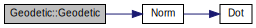
\includegraphics[width=328pt]{classGeodetic_ad813b9417dac1cee7ea962c36b82bb9c_cgraph}
\end{center}
\end{figure}




\subsection{Member Function Documentation}
\hypertarget{classGeodetic_a47d84f3c9f36b3443cea7c344fcfbddc}{\index{Geodetic@{Geodetic}!L\-T\-C\-\_\-\-Matrix@{L\-T\-C\-\_\-\-Matrix}}
\index{L\-T\-C\-\_\-\-Matrix@{L\-T\-C\-\_\-\-Matrix}!Geodetic@{Geodetic}}
\subsubsection[{L\-T\-C\-\_\-\-Matrix}]{\setlength{\rightskip}{0pt plus 5cm}{\bf Matrix} Geodetic\-::\-L\-T\-C\-\_\-\-Matrix (
\begin{DoxyParamCaption}
{}
\end{DoxyParamCaption}
) const}}\label{classGeodetic_a47d84f3c9f36b3443cea7c344fcfbddc}


Definition at line 723 of file S\-A\-T\-\_\-\-Ref\-Sys.\-cpp.



Here is the call graph for this function\-:\nopagebreak
\begin{figure}[H]
\begin{center}
\leavevmode
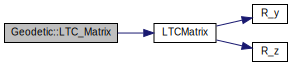
\includegraphics[width=350pt]{classGeodetic_a47d84f3c9f36b3443cea7c344fcfbddc_cgraph}
\end{center}
\end{figure}




Here is the caller graph for this function\-:\nopagebreak
\begin{figure}[H]
\begin{center}
\leavevmode
\includegraphics[width=268pt]{classGeodetic_a47d84f3c9f36b3443cea7c344fcfbddc_icgraph}
\end{center}
\end{figure}


\hypertarget{classGeodetic_a7c02e1089d2fc2eebd46a20252e78130}{\index{Geodetic@{Geodetic}!Position@{Position}}
\index{Position@{Position}!Geodetic@{Geodetic}}
\subsubsection[{Position}]{\setlength{\rightskip}{0pt plus 5cm}{\bf Vector} Geodetic\-::\-Position (
\begin{DoxyParamCaption}
\item[{double}]{R\-\_\-equ = {\ttfamily {\bf R\-\_\-\-Earth}}, }
\item[{double}]{f = {\ttfamily {\bf f\-\_\-\-Earth}}}
\end{DoxyParamCaption}
) const}}\label{classGeodetic_a7c02e1089d2fc2eebd46a20252e78130}


Definition at line 697 of file S\-A\-T\-\_\-\-Ref\-Sys.\-cpp.



Here is the caller graph for this function\-:\nopagebreak
\begin{figure}[H]
\begin{center}
\leavevmode
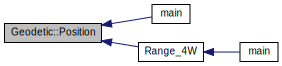
\includegraphics[width=350pt]{classGeodetic_a7c02e1089d2fc2eebd46a20252e78130_icgraph}
\end{center}
\end{figure}




\subsection{Member Data Documentation}
\hypertarget{classGeodetic_a7e0792c8e2f5fa75821a5b0ad94d5242}{\index{Geodetic@{Geodetic}!h@{h}}
\index{h@{h}!Geodetic@{Geodetic}}
\subsubsection[{h}]{\setlength{\rightskip}{0pt plus 5cm}double Geodetic\-::h}}\label{classGeodetic_a7e0792c8e2f5fa75821a5b0ad94d5242}


Definition at line 271 of file S\-A\-T\-\_\-\-Ref\-Sys.\-h.

\hypertarget{classGeodetic_a7e1fb26747be20d8c48009c8d5caa272}{\index{Geodetic@{Geodetic}!lat@{lat}}
\index{lat@{lat}!Geodetic@{Geodetic}}
\subsubsection[{lat}]{\setlength{\rightskip}{0pt plus 5cm}double Geodetic\-::lat}}\label{classGeodetic_a7e1fb26747be20d8c48009c8d5caa272}


Definition at line 270 of file S\-A\-T\-\_\-\-Ref\-Sys.\-h.

\hypertarget{classGeodetic_a59a979c3f60a77eb5f2ac80f374f7d23}{\index{Geodetic@{Geodetic}!lon@{lon}}
\index{lon@{lon}!Geodetic@{Geodetic}}
\subsubsection[{lon}]{\setlength{\rightskip}{0pt plus 5cm}double Geodetic\-::lon}}\label{classGeodetic_a59a979c3f60a77eb5f2ac80f374f7d23}


Definition at line 269 of file S\-A\-T\-\_\-\-Ref\-Sys.\-h.



The documentation for this class was generated from the following files\-:\begin{DoxyCompactItemize}
\item 
\hyperlink{SAT__RefSys_8h}{S\-A\-T\-\_\-\-Ref\-Sys.\-h}\item 
\hyperlink{SAT__RefSys_8cpp}{S\-A\-T\-\_\-\-Ref\-Sys.\-cpp}\end{DoxyCompactItemize}

\hypertarget{structGravModel}{\section{Grav\-Model Struct Reference}
\label{structGravModel}\index{Grav\-Model@{Grav\-Model}}
}


{\ttfamily \#include $<$S\-A\-T\-\_\-\-Force.\-h$>$}



Collaboration diagram for Grav\-Model\-:\nopagebreak
\begin{figure}[H]
\begin{center}
\leavevmode
\includegraphics[width=144pt]{structGravModel__coll__graph}
\end{center}
\end{figure}
\subsection*{Public Member Functions}
\begin{DoxyCompactItemize}
\item 
\hyperlink{structGravModel_a0497787562c367ca5f322d23885df1c1}{Grav\-Model} (int n, double gm, double r\-\_\-ref, const double $\ast$p\-\_\-cs)
\end{DoxyCompactItemize}
\subsection*{Public Attributes}
\begin{DoxyCompactItemize}
\item 
int \hyperlink{structGravModel_a2523255eb438cc2d4d7166d01abbb805}{n\-\_\-max}
\item 
int \hyperlink{structGravModel_a77ed9c234c938a6ebb239df2174df476}{m\-\_\-max}
\item 
double \hyperlink{structGravModel_a138296eb0d0cdfd86615872e09db9382}{G\-M}
\item 
double \hyperlink{structGravModel_ad1690c2e76a4b250fa68a42ebc495cec}{R\-\_\-ref}
\item 
\hyperlink{classMatrix}{Matrix} \hyperlink{structGravModel_a6c399c91b140cef19ed5ebfc9117cffb}{C\-S}
\end{DoxyCompactItemize}


\subsection{Detailed Description}


Definition at line 39 of file S\-A\-T\-\_\-\-Force.\-h.



\subsection{Constructor \& Destructor Documentation}
\hypertarget{structGravModel_a0497787562c367ca5f322d23885df1c1}{\index{Grav\-Model@{Grav\-Model}!Grav\-Model@{Grav\-Model}}
\index{Grav\-Model@{Grav\-Model}!GravModel@{Grav\-Model}}
\subsubsection[{Grav\-Model}]{\setlength{\rightskip}{0pt plus 5cm}Grav\-Model\-::\-Grav\-Model (
\begin{DoxyParamCaption}
\item[{int}]{n, }
\item[{double}]{gm, }
\item[{double}]{r\-\_\-ref, }
\item[{const double $\ast$}]{p\-\_\-cs}
\end{DoxyParamCaption}
)\hspace{0.3cm}{\ttfamily [inline]}}}\label{structGravModel_a0497787562c367ca5f322d23885df1c1}


Definition at line 48 of file S\-A\-T\-\_\-\-Force.\-h.



\subsection{Member Data Documentation}
\hypertarget{structGravModel_a6c399c91b140cef19ed5ebfc9117cffb}{\index{Grav\-Model@{Grav\-Model}!C\-S@{C\-S}}
\index{C\-S@{C\-S}!GravModel@{Grav\-Model}}
\subsubsection[{C\-S}]{\setlength{\rightskip}{0pt plus 5cm}{\bf Matrix} Grav\-Model\-::\-C\-S}}\label{structGravModel_a6c399c91b140cef19ed5ebfc9117cffb}


Definition at line 45 of file S\-A\-T\-\_\-\-Force.\-h.

\hypertarget{structGravModel_a138296eb0d0cdfd86615872e09db9382}{\index{Grav\-Model@{Grav\-Model}!G\-M@{G\-M}}
\index{G\-M@{G\-M}!GravModel@{Grav\-Model}}
\subsubsection[{G\-M}]{\setlength{\rightskip}{0pt plus 5cm}double Grav\-Model\-::\-G\-M}}\label{structGravModel_a138296eb0d0cdfd86615872e09db9382}


Definition at line 43 of file S\-A\-T\-\_\-\-Force.\-h.

\hypertarget{structGravModel_a77ed9c234c938a6ebb239df2174df476}{\index{Grav\-Model@{Grav\-Model}!m\-\_\-max@{m\-\_\-max}}
\index{m\-\_\-max@{m\-\_\-max}!GravModel@{Grav\-Model}}
\subsubsection[{m\-\_\-max}]{\setlength{\rightskip}{0pt plus 5cm}int Grav\-Model\-::m\-\_\-max}}\label{structGravModel_a77ed9c234c938a6ebb239df2174df476}


Definition at line 42 of file S\-A\-T\-\_\-\-Force.\-h.

\hypertarget{structGravModel_a2523255eb438cc2d4d7166d01abbb805}{\index{Grav\-Model@{Grav\-Model}!n\-\_\-max@{n\-\_\-max}}
\index{n\-\_\-max@{n\-\_\-max}!GravModel@{Grav\-Model}}
\subsubsection[{n\-\_\-max}]{\setlength{\rightskip}{0pt plus 5cm}int Grav\-Model\-::n\-\_\-max}}\label{structGravModel_a2523255eb438cc2d4d7166d01abbb805}


Definition at line 41 of file S\-A\-T\-\_\-\-Force.\-h.

\hypertarget{structGravModel_ad1690c2e76a4b250fa68a42ebc495cec}{\index{Grav\-Model@{Grav\-Model}!R\-\_\-ref@{R\-\_\-ref}}
\index{R\-\_\-ref@{R\-\_\-ref}!GravModel@{Grav\-Model}}
\subsubsection[{R\-\_\-ref}]{\setlength{\rightskip}{0pt plus 5cm}double Grav\-Model\-::\-R\-\_\-ref}}\label{structGravModel_ad1690c2e76a4b250fa68a42ebc495cec}


Definition at line 44 of file S\-A\-T\-\_\-\-Force.\-h.



The documentation for this struct was generated from the following file\-:\begin{DoxyCompactItemize}
\item 
\hyperlink{SAT__Force_8h}{S\-A\-T\-\_\-\-Force.\-h}\end{DoxyCompactItemize}

\hypertarget{classIERS}{\section{I\-E\-R\-S Class Reference}
\label{classIERS}\index{I\-E\-R\-S@{I\-E\-R\-S}}
}


{\ttfamily \#include $<$S\-A\-T\-\_\-\-Ref\-Sys.\-h$>$}

\subsection*{Static Public Member Functions}
\begin{DoxyCompactItemize}
\item 
static void \hyperlink{classIERS_ae1161daecc9629cdb716884cef9d1fa9}{Set} (double \hyperlink{classIERS_a2601a074a58e3c470db336bc1aea6791}{U\-T1\-\_\-\-U\-T\-C}, double \hyperlink{classIERS_ad872e267797cb8d5be328b236287565f}{U\-T\-C\-\_\-\-T\-A\-I}, double \hyperlink{classIERS_aa6619a8885c83540cf92a32510285edb}{x\-\_\-pole}, double \hyperlink{classIERS_a685869b1f1ac92c0595f8be01307a2ce}{y\-\_\-pole})
\item 
static double \hyperlink{classIERS_ad872e267797cb8d5be328b236287565f}{U\-T\-C\-\_\-\-T\-A\-I} (double Mjd\-\_\-\-U\-T\-C)
\item 
static double \hyperlink{classIERS_acfce0b1a43896fed7b1bf9cefe3baebd}{U\-T1\-\_\-\-T\-A\-I} (double Mjd\-\_\-\-U\-T\-C)
\item 
static double \hyperlink{classIERS_af3a179849d1bd691235472984ffa1995}{U\-T\-C\-\_\-\-G\-P\-S} (double Mjd\-\_\-\-U\-T\-C)
\item 
static double \hyperlink{classIERS_a64350c76a5faed69b9ac10b8ab3f869c}{U\-T1\-\_\-\-G\-P\-S} (double Mjd\-\_\-\-U\-T\-C)
\item 
static double \hyperlink{classIERS_abe17029c05804e5886ae14eae119c0f1}{T\-T\-\_\-\-U\-T\-C} (double Mjd\-\_\-\-U\-T\-C)
\item 
static double \hyperlink{classIERS_a2d0dcfa406b6f5c81ccbc71cb2cb5525}{T\-A\-I\-\_\-\-U\-T\-C} (double Mjd\-\_\-\-U\-T\-C)
\item 
static double \hyperlink{classIERS_a79c2d9fcfafe0c0d8cee4545e17af0f3}{G\-P\-S\-\_\-\-U\-T\-C} (double Mjd\-\_\-\-U\-T\-C)
\item 
static double \hyperlink{classIERS_a2601a074a58e3c470db336bc1aea6791}{U\-T1\-\_\-\-U\-T\-C} (double Mjd\-\_\-\-U\-T\-C)
\item 
static double \hyperlink{classIERS_aa6619a8885c83540cf92a32510285edb}{x\-\_\-pole} (double Mjd\-\_\-\-U\-T\-C)
\item 
static double \hyperlink{classIERS_a685869b1f1ac92c0595f8be01307a2ce}{y\-\_\-pole} (double Mjd\-\_\-\-U\-T\-C)
\end{DoxyCompactItemize}
\subsection*{Static Public Attributes}
\begin{DoxyCompactItemize}
\item 
static const double \hyperlink{classIERS_ab6b095690199dc9789b668eafe93423e}{T\-T\-\_\-\-T\-A\-I} = +32.\-184
\item 
static const double \hyperlink{classIERS_a6289aefd6f6c45e58d7d9ce2e3789c64}{G\-P\-S\-\_\-\-T\-A\-I} = -\/19.\-0
\item 
static const double \hyperlink{classIERS_aa3e35ab4212b649feeaf61764d85c690}{T\-T\-\_\-\-G\-P\-S}
\item 
static const double \hyperlink{classIERS_a7bf84e2e1ee0b01fcfcc4e6e2fe35355}{T\-A\-I\-\_\-\-G\-P\-S} = -\/\hyperlink{classIERS_a6289aefd6f6c45e58d7d9ce2e3789c64}{I\-E\-R\-S\-::\-G\-P\-S\-\_\-\-T\-A\-I}
\end{DoxyCompactItemize}
\subsection*{Static Private Attributes}
\begin{DoxyCompactItemize}
\item 
static double \hyperlink{classIERS_a75a822b27f30fc3369697819de08da84}{U\-T1\-\_\-\-T\-A\-I\-\_\-} = 0.\-0
\item 
static double \hyperlink{classIERS_a4df9d5b7347defccc192c1ab5c437e35}{U\-T\-C\-\_\-\-T\-A\-I\-\_\-} = 0.\-0
\item 
static double \hyperlink{classIERS_ac8c79654837cc32556a29a6d9597f3e8}{x\-\_\-pole\-\_\-} = 0.\-0
\item 
static double \hyperlink{classIERS_a359e82751a2edfbc9d8fe6fa7a9d8061}{y\-\_\-pole\-\_\-} = 0.\-0
\end{DoxyCompactItemize}


\subsection{Detailed Description}


Definition at line 47 of file S\-A\-T\-\_\-\-Ref\-Sys.\-h.



\subsection{Member Function Documentation}
\hypertarget{classIERS_a79c2d9fcfafe0c0d8cee4545e17af0f3}{\index{I\-E\-R\-S@{I\-E\-R\-S}!G\-P\-S\-\_\-\-U\-T\-C@{G\-P\-S\-\_\-\-U\-T\-C}}
\index{G\-P\-S\-\_\-\-U\-T\-C@{G\-P\-S\-\_\-\-U\-T\-C}!IERS@{I\-E\-R\-S}}
\subsubsection[{G\-P\-S\-\_\-\-U\-T\-C}]{\setlength{\rightskip}{0pt plus 5cm}double I\-E\-R\-S\-::\-G\-P\-S\-\_\-\-U\-T\-C (
\begin{DoxyParamCaption}
\item[{double}]{Mjd\-\_\-\-U\-T\-C}
\end{DoxyParamCaption}
)\hspace{0.3cm}{\ttfamily [static]}}}\label{classIERS_a79c2d9fcfafe0c0d8cee4545e17af0f3}


Definition at line 113 of file S\-A\-T\-\_\-\-Ref\-Sys.\-cpp.



Here is the call graph for this function\-:\nopagebreak
\begin{figure}[H]
\begin{center}
\leavevmode
\includegraphics[width=300pt]{classIERS_a79c2d9fcfafe0c0d8cee4545e17af0f3_cgraph}
\end{center}
\end{figure}




Here is the caller graph for this function\-:\nopagebreak
\begin{figure}[H]
\begin{center}
\leavevmode
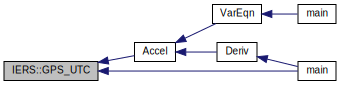
\includegraphics[width=350pt]{classIERS_a79c2d9fcfafe0c0d8cee4545e17af0f3_icgraph}
\end{center}
\end{figure}


\hypertarget{classIERS_ae1161daecc9629cdb716884cef9d1fa9}{\index{I\-E\-R\-S@{I\-E\-R\-S}!Set@{Set}}
\index{Set@{Set}!IERS@{I\-E\-R\-S}}
\subsubsection[{Set}]{\setlength{\rightskip}{0pt plus 5cm}void I\-E\-R\-S\-::\-Set (
\begin{DoxyParamCaption}
\item[{double}]{U\-T1\-\_\-\-U\-T\-C, }
\item[{double}]{U\-T\-C\-\_\-\-T\-A\-I, }
\item[{double}]{x\-\_\-pole, }
\item[{double}]{y\-\_\-pole}
\end{DoxyParamCaption}
)\hspace{0.3cm}{\ttfamily [static]}}}\label{classIERS_ae1161daecc9629cdb716884cef9d1fa9}


Definition at line 95 of file S\-A\-T\-\_\-\-Ref\-Sys.\-cpp.



Here is the call graph for this function\-:\nopagebreak
\begin{figure}[H]
\begin{center}
\leavevmode
\includegraphics[width=268pt]{classIERS_ae1161daecc9629cdb716884cef9d1fa9_cgraph}
\end{center}
\end{figure}




Here is the caller graph for this function\-:\nopagebreak
\begin{figure}[H]
\begin{center}
\leavevmode
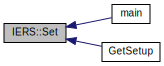
\includegraphics[width=236pt]{classIERS_ae1161daecc9629cdb716884cef9d1fa9_icgraph}
\end{center}
\end{figure}


\hypertarget{classIERS_a2d0dcfa406b6f5c81ccbc71cb2cb5525}{\index{I\-E\-R\-S@{I\-E\-R\-S}!T\-A\-I\-\_\-\-U\-T\-C@{T\-A\-I\-\_\-\-U\-T\-C}}
\index{T\-A\-I\-\_\-\-U\-T\-C@{T\-A\-I\-\_\-\-U\-T\-C}!IERS@{I\-E\-R\-S}}
\subsubsection[{T\-A\-I\-\_\-\-U\-T\-C}]{\setlength{\rightskip}{0pt plus 5cm}static double I\-E\-R\-S\-::\-T\-A\-I\-\_\-\-U\-T\-C (
\begin{DoxyParamCaption}
\item[{double}]{Mjd\-\_\-\-U\-T\-C}
\end{DoxyParamCaption}
)\hspace{0.3cm}{\ttfamily [static]}}}\label{classIERS_a2d0dcfa406b6f5c81ccbc71cb2cb5525}
\hypertarget{classIERS_abe17029c05804e5886ae14eae119c0f1}{\index{I\-E\-R\-S@{I\-E\-R\-S}!T\-T\-\_\-\-U\-T\-C@{T\-T\-\_\-\-U\-T\-C}}
\index{T\-T\-\_\-\-U\-T\-C@{T\-T\-\_\-\-U\-T\-C}!IERS@{I\-E\-R\-S}}
\subsubsection[{T\-T\-\_\-\-U\-T\-C}]{\setlength{\rightskip}{0pt plus 5cm}double I\-E\-R\-S\-::\-T\-T\-\_\-\-U\-T\-C (
\begin{DoxyParamCaption}
\item[{double}]{Mjd\-\_\-\-U\-T\-C}
\end{DoxyParamCaption}
)\hspace{0.3cm}{\ttfamily [static]}}}\label{classIERS_abe17029c05804e5886ae14eae119c0f1}


Definition at line 112 of file S\-A\-T\-\_\-\-Ref\-Sys.\-cpp.



Here is the call graph for this function\-:\nopagebreak
\begin{figure}[H]
\begin{center}
\leavevmode
\includegraphics[width=292pt]{classIERS_abe17029c05804e5886ae14eae119c0f1_cgraph}
\end{center}
\end{figure}




Here is the caller graph for this function\-:\nopagebreak
\begin{figure}[H]
\begin{center}
\leavevmode
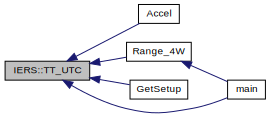
\includegraphics[width=342pt]{classIERS_abe17029c05804e5886ae14eae119c0f1_icgraph}
\end{center}
\end{figure}


\hypertarget{classIERS_a64350c76a5faed69b9ac10b8ab3f869c}{\index{I\-E\-R\-S@{I\-E\-R\-S}!U\-T1\-\_\-\-G\-P\-S@{U\-T1\-\_\-\-G\-P\-S}}
\index{U\-T1\-\_\-\-G\-P\-S@{U\-T1\-\_\-\-G\-P\-S}!IERS@{I\-E\-R\-S}}
\subsubsection[{U\-T1\-\_\-\-G\-P\-S}]{\setlength{\rightskip}{0pt plus 5cm}double I\-E\-R\-S\-::\-U\-T1\-\_\-\-G\-P\-S (
\begin{DoxyParamCaption}
\item[{double}]{Mjd\-\_\-\-U\-T\-C}
\end{DoxyParamCaption}
)\hspace{0.3cm}{\ttfamily [static]}}}\label{classIERS_a64350c76a5faed69b9ac10b8ab3f869c}


Definition at line 110 of file S\-A\-T\-\_\-\-Ref\-Sys.\-cpp.



Here is the call graph for this function\-:\nopagebreak
\begin{figure}[H]
\begin{center}
\leavevmode
\includegraphics[width=294pt]{classIERS_a64350c76a5faed69b9ac10b8ab3f869c_cgraph}
\end{center}
\end{figure}


\hypertarget{classIERS_acfce0b1a43896fed7b1bf9cefe3baebd}{\index{I\-E\-R\-S@{I\-E\-R\-S}!U\-T1\-\_\-\-T\-A\-I@{U\-T1\-\_\-\-T\-A\-I}}
\index{U\-T1\-\_\-\-T\-A\-I@{U\-T1\-\_\-\-T\-A\-I}!IERS@{I\-E\-R\-S}}
\subsubsection[{U\-T1\-\_\-\-T\-A\-I}]{\setlength{\rightskip}{0pt plus 5cm}double I\-E\-R\-S\-::\-U\-T1\-\_\-\-T\-A\-I (
\begin{DoxyParamCaption}
\item[{double}]{Mjd\-\_\-\-U\-T\-C}
\end{DoxyParamCaption}
)\hspace{0.3cm}{\ttfamily [static]}}}\label{classIERS_acfce0b1a43896fed7b1bf9cefe3baebd}


Definition at line 107 of file S\-A\-T\-\_\-\-Ref\-Sys.\-cpp.



Here is the caller graph for this function\-:\nopagebreak
\begin{figure}[H]
\begin{center}
\leavevmode
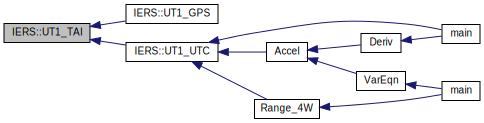
\includegraphics[width=350pt]{classIERS_acfce0b1a43896fed7b1bf9cefe3baebd_icgraph}
\end{center}
\end{figure}


\hypertarget{classIERS_a2601a074a58e3c470db336bc1aea6791}{\index{I\-E\-R\-S@{I\-E\-R\-S}!U\-T1\-\_\-\-U\-T\-C@{U\-T1\-\_\-\-U\-T\-C}}
\index{U\-T1\-\_\-\-U\-T\-C@{U\-T1\-\_\-\-U\-T\-C}!IERS@{I\-E\-R\-S}}
\subsubsection[{U\-T1\-\_\-\-U\-T\-C}]{\setlength{\rightskip}{0pt plus 5cm}double I\-E\-R\-S\-::\-U\-T1\-\_\-\-U\-T\-C (
\begin{DoxyParamCaption}
\item[{double}]{Mjd\-\_\-\-U\-T\-C}
\end{DoxyParamCaption}
)\hspace{0.3cm}{\ttfamily [static]}}}\label{classIERS_a2601a074a58e3c470db336bc1aea6791}


Definition at line 114 of file S\-A\-T\-\_\-\-Ref\-Sys.\-cpp.



Here is the call graph for this function\-:\nopagebreak
\begin{figure}[H]
\begin{center}
\leavevmode
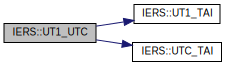
\includegraphics[width=298pt]{classIERS_a2601a074a58e3c470db336bc1aea6791_cgraph}
\end{center}
\end{figure}




Here is the caller graph for this function\-:\nopagebreak
\begin{figure}[H]
\begin{center}
\leavevmode
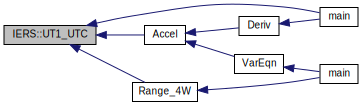
\includegraphics[width=350pt]{classIERS_a2601a074a58e3c470db336bc1aea6791_icgraph}
\end{center}
\end{figure}


\hypertarget{classIERS_af3a179849d1bd691235472984ffa1995}{\index{I\-E\-R\-S@{I\-E\-R\-S}!U\-T\-C\-\_\-\-G\-P\-S@{U\-T\-C\-\_\-\-G\-P\-S}}
\index{U\-T\-C\-\_\-\-G\-P\-S@{U\-T\-C\-\_\-\-G\-P\-S}!IERS@{I\-E\-R\-S}}
\subsubsection[{U\-T\-C\-\_\-\-G\-P\-S}]{\setlength{\rightskip}{0pt plus 5cm}double I\-E\-R\-S\-::\-U\-T\-C\-\_\-\-G\-P\-S (
\begin{DoxyParamCaption}
\item[{double}]{Mjd\-\_\-\-U\-T\-C}
\end{DoxyParamCaption}
)\hspace{0.3cm}{\ttfamily [static]}}}\label{classIERS_af3a179849d1bd691235472984ffa1995}


Definition at line 109 of file S\-A\-T\-\_\-\-Ref\-Sys.\-cpp.



Here is the call graph for this function\-:\nopagebreak
\begin{figure}[H]
\begin{center}
\leavevmode
\includegraphics[width=300pt]{classIERS_af3a179849d1bd691235472984ffa1995_cgraph}
\end{center}
\end{figure}


\hypertarget{classIERS_ad872e267797cb8d5be328b236287565f}{\index{I\-E\-R\-S@{I\-E\-R\-S}!U\-T\-C\-\_\-\-T\-A\-I@{U\-T\-C\-\_\-\-T\-A\-I}}
\index{U\-T\-C\-\_\-\-T\-A\-I@{U\-T\-C\-\_\-\-T\-A\-I}!IERS@{I\-E\-R\-S}}
\subsubsection[{U\-T\-C\-\_\-\-T\-A\-I}]{\setlength{\rightskip}{0pt plus 5cm}double I\-E\-R\-S\-::\-U\-T\-C\-\_\-\-T\-A\-I (
\begin{DoxyParamCaption}
\item[{double}]{Mjd\-\_\-\-U\-T\-C}
\end{DoxyParamCaption}
)\hspace{0.3cm}{\ttfamily [static]}}}\label{classIERS_ad872e267797cb8d5be328b236287565f}


Definition at line 106 of file S\-A\-T\-\_\-\-Ref\-Sys.\-cpp.



Here is the caller graph for this function\-:\nopagebreak
\begin{figure}[H]
\begin{center}
\leavevmode
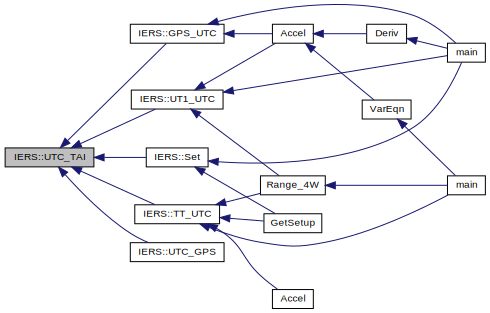
\includegraphics[width=350pt]{classIERS_ad872e267797cb8d5be328b236287565f_icgraph}
\end{center}
\end{figure}


\hypertarget{classIERS_aa6619a8885c83540cf92a32510285edb}{\index{I\-E\-R\-S@{I\-E\-R\-S}!x\-\_\-pole@{x\-\_\-pole}}
\index{x\-\_\-pole@{x\-\_\-pole}!IERS@{I\-E\-R\-S}}
\subsubsection[{x\-\_\-pole}]{\setlength{\rightskip}{0pt plus 5cm}double I\-E\-R\-S\-::x\-\_\-pole (
\begin{DoxyParamCaption}
\item[{double}]{Mjd\-\_\-\-U\-T\-C}
\end{DoxyParamCaption}
)\hspace{0.3cm}{\ttfamily [static]}}}\label{classIERS_aa6619a8885c83540cf92a32510285edb}


Definition at line 121 of file S\-A\-T\-\_\-\-Ref\-Sys.\-cpp.



Here is the caller graph for this function\-:\nopagebreak
\begin{figure}[H]
\begin{center}
\leavevmode
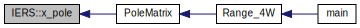
\includegraphics[width=350pt]{classIERS_aa6619a8885c83540cf92a32510285edb_icgraph}
\end{center}
\end{figure}


\hypertarget{classIERS_a685869b1f1ac92c0595f8be01307a2ce}{\index{I\-E\-R\-S@{I\-E\-R\-S}!y\-\_\-pole@{y\-\_\-pole}}
\index{y\-\_\-pole@{y\-\_\-pole}!IERS@{I\-E\-R\-S}}
\subsubsection[{y\-\_\-pole}]{\setlength{\rightskip}{0pt plus 5cm}double I\-E\-R\-S\-::y\-\_\-pole (
\begin{DoxyParamCaption}
\item[{double}]{Mjd\-\_\-\-U\-T\-C}
\end{DoxyParamCaption}
)\hspace{0.3cm}{\ttfamily [static]}}}\label{classIERS_a685869b1f1ac92c0595f8be01307a2ce}


Definition at line 125 of file S\-A\-T\-\_\-\-Ref\-Sys.\-cpp.



Here is the caller graph for this function\-:\nopagebreak
\begin{figure}[H]
\begin{center}
\leavevmode
\includegraphics[width=350pt]{classIERS_a685869b1f1ac92c0595f8be01307a2ce_icgraph}
\end{center}
\end{figure}




\subsection{Member Data Documentation}
\hypertarget{classIERS_a6289aefd6f6c45e58d7d9ce2e3789c64}{\index{I\-E\-R\-S@{I\-E\-R\-S}!G\-P\-S\-\_\-\-T\-A\-I@{G\-P\-S\-\_\-\-T\-A\-I}}
\index{G\-P\-S\-\_\-\-T\-A\-I@{G\-P\-S\-\_\-\-T\-A\-I}!IERS@{I\-E\-R\-S}}
\subsubsection[{G\-P\-S\-\_\-\-T\-A\-I}]{\setlength{\rightskip}{0pt plus 5cm}const double I\-E\-R\-S\-::\-G\-P\-S\-\_\-\-T\-A\-I = -\/19.\-0\hspace{0.3cm}{\ttfamily [static]}}}\label{classIERS_a6289aefd6f6c45e58d7d9ce2e3789c64}


Definition at line 57 of file S\-A\-T\-\_\-\-Ref\-Sys.\-h.

\hypertarget{classIERS_a7bf84e2e1ee0b01fcfcc4e6e2fe35355}{\index{I\-E\-R\-S@{I\-E\-R\-S}!T\-A\-I\-\_\-\-G\-P\-S@{T\-A\-I\-\_\-\-G\-P\-S}}
\index{T\-A\-I\-\_\-\-G\-P\-S@{T\-A\-I\-\_\-\-G\-P\-S}!IERS@{I\-E\-R\-S}}
\subsubsection[{T\-A\-I\-\_\-\-G\-P\-S}]{\setlength{\rightskip}{0pt plus 5cm}const double I\-E\-R\-S\-::\-T\-A\-I\-\_\-\-G\-P\-S = -\/{\bf I\-E\-R\-S\-::\-G\-P\-S\-\_\-\-T\-A\-I}\hspace{0.3cm}{\ttfamily [static]}}}\label{classIERS_a7bf84e2e1ee0b01fcfcc4e6e2fe35355}


Definition at line 62 of file S\-A\-T\-\_\-\-Ref\-Sys.\-h.

\hypertarget{classIERS_aa3e35ab4212b649feeaf61764d85c690}{\index{I\-E\-R\-S@{I\-E\-R\-S}!T\-T\-\_\-\-G\-P\-S@{T\-T\-\_\-\-G\-P\-S}}
\index{T\-T\-\_\-\-G\-P\-S@{T\-T\-\_\-\-G\-P\-S}!IERS@{I\-E\-R\-S}}
\subsubsection[{T\-T\-\_\-\-G\-P\-S}]{\setlength{\rightskip}{0pt plus 5cm}const double I\-E\-R\-S\-::\-T\-T\-\_\-\-G\-P\-S\hspace{0.3cm}{\ttfamily [static]}}}\label{classIERS_aa3e35ab4212b649feeaf61764d85c690}
{\bfseries Initial value\-:}
\begin{DoxyCode}
=  \hyperlink{classIERS_ab6b095690199dc9789b668eafe93423e}{IERS::TT\_TAI}     
                             -\hyperlink{classIERS_a6289aefd6f6c45e58d7d9ce2e3789c64}{IERS::GPS\_TAI}
\end{DoxyCode}


Definition at line 61 of file S\-A\-T\-\_\-\-Ref\-Sys.\-h.

\hypertarget{classIERS_ab6b095690199dc9789b668eafe93423e}{\index{I\-E\-R\-S@{I\-E\-R\-S}!T\-T\-\_\-\-T\-A\-I@{T\-T\-\_\-\-T\-A\-I}}
\index{T\-T\-\_\-\-T\-A\-I@{T\-T\-\_\-\-T\-A\-I}!IERS@{I\-E\-R\-S}}
\subsubsection[{T\-T\-\_\-\-T\-A\-I}]{\setlength{\rightskip}{0pt plus 5cm}const double I\-E\-R\-S\-::\-T\-T\-\_\-\-T\-A\-I = +32.\-184\hspace{0.3cm}{\ttfamily [static]}}}\label{classIERS_ab6b095690199dc9789b668eafe93423e}


Definition at line 56 of file S\-A\-T\-\_\-\-Ref\-Sys.\-h.

\hypertarget{classIERS_a75a822b27f30fc3369697819de08da84}{\index{I\-E\-R\-S@{I\-E\-R\-S}!U\-T1\-\_\-\-T\-A\-I\-\_\-@{U\-T1\-\_\-\-T\-A\-I\-\_\-}}
\index{U\-T1\-\_\-\-T\-A\-I\-\_\-@{U\-T1\-\_\-\-T\-A\-I\-\_\-}!IERS@{I\-E\-R\-S}}
\subsubsection[{U\-T1\-\_\-\-T\-A\-I\-\_\-}]{\setlength{\rightskip}{0pt plus 5cm}double I\-E\-R\-S\-::\-U\-T1\-\_\-\-T\-A\-I\-\_\- = 0.\-0\hspace{0.3cm}{\ttfamily [static]}, {\ttfamily [private]}}}\label{classIERS_a75a822b27f30fc3369697819de08da84}


Definition at line 75 of file S\-A\-T\-\_\-\-Ref\-Sys.\-h.

\hypertarget{classIERS_a4df9d5b7347defccc192c1ab5c437e35}{\index{I\-E\-R\-S@{I\-E\-R\-S}!U\-T\-C\-\_\-\-T\-A\-I\-\_\-@{U\-T\-C\-\_\-\-T\-A\-I\-\_\-}}
\index{U\-T\-C\-\_\-\-T\-A\-I\-\_\-@{U\-T\-C\-\_\-\-T\-A\-I\-\_\-}!IERS@{I\-E\-R\-S}}
\subsubsection[{U\-T\-C\-\_\-\-T\-A\-I\-\_\-}]{\setlength{\rightskip}{0pt plus 5cm}double I\-E\-R\-S\-::\-U\-T\-C\-\_\-\-T\-A\-I\-\_\- = 0.\-0\hspace{0.3cm}{\ttfamily [static]}, {\ttfamily [private]}}}\label{classIERS_a4df9d5b7347defccc192c1ab5c437e35}


Definition at line 76 of file S\-A\-T\-\_\-\-Ref\-Sys.\-h.

\hypertarget{classIERS_ac8c79654837cc32556a29a6d9597f3e8}{\index{I\-E\-R\-S@{I\-E\-R\-S}!x\-\_\-pole\-\_\-@{x\-\_\-pole\-\_\-}}
\index{x\-\_\-pole\-\_\-@{x\-\_\-pole\-\_\-}!IERS@{I\-E\-R\-S}}
\subsubsection[{x\-\_\-pole\-\_\-}]{\setlength{\rightskip}{0pt plus 5cm}double I\-E\-R\-S\-::x\-\_\-pole\-\_\- = 0.\-0\hspace{0.3cm}{\ttfamily [static]}, {\ttfamily [private]}}}\label{classIERS_ac8c79654837cc32556a29a6d9597f3e8}


Definition at line 77 of file S\-A\-T\-\_\-\-Ref\-Sys.\-h.

\hypertarget{classIERS_a359e82751a2edfbc9d8fe6fa7a9d8061}{\index{I\-E\-R\-S@{I\-E\-R\-S}!y\-\_\-pole\-\_\-@{y\-\_\-pole\-\_\-}}
\index{y\-\_\-pole\-\_\-@{y\-\_\-pole\-\_\-}!IERS@{I\-E\-R\-S}}
\subsubsection[{y\-\_\-pole\-\_\-}]{\setlength{\rightskip}{0pt plus 5cm}double I\-E\-R\-S\-::y\-\_\-pole\-\_\- = 0.\-0\hspace{0.3cm}{\ttfamily [static]}, {\ttfamily [private]}}}\label{classIERS_a359e82751a2edfbc9d8fe6fa7a9d8061}


Definition at line 78 of file S\-A\-T\-\_\-\-Ref\-Sys.\-h.



The documentation for this class was generated from the following files\-:\begin{DoxyCompactItemize}
\item 
\hyperlink{SAT__RefSys_8h}{S\-A\-T\-\_\-\-Ref\-Sys.\-h}\item 
\hyperlink{SAT__RefSys_8cpp}{S\-A\-T\-\_\-\-Ref\-Sys.\-cpp}\end{DoxyCompactItemize}

\hypertarget{classLSQ}{\section{L\-S\-Q Class Reference}
\label{classLSQ}\index{L\-S\-Q@{L\-S\-Q}}
}


{\ttfamily \#include $<$S\-A\-T\-\_\-\-Filter.\-h$>$}



Collaboration diagram for L\-S\-Q\-:\nopagebreak
\begin{figure}[H]
\begin{center}
\leavevmode
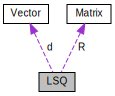
\includegraphics[width=187pt]{classLSQ__coll__graph}
\end{center}
\end{figure}
\subsection*{Public Member Functions}
\begin{DoxyCompactItemize}
\item 
\hyperlink{classLSQ_a07c17e3f379fb18c8a5c4c197495834a}{L\-S\-Q} (int n\-Est)
\item 
int \hyperlink{classLSQ_afa6fe2b1d00b6ef2ced1089426d6c668}{n\-Data} ()
\item 
void \hyperlink{classLSQ_a77940543ea83db4f557cdf09f99b3098}{Init} ()
\item 
void \hyperlink{classLSQ_a5a2fdaddfaeaf4638bfaafc25a6ae793}{Init} (const \hyperlink{classVector}{Vector} \&x, const \hyperlink{classMatrix}{Matrix} \&P)
\item 
void \hyperlink{classLSQ_aa98a7935493ef8e5cfc6f21cb6920307}{Accumulate} (const \hyperlink{classVector}{Vector} \&A, double b, double sigma=1.\-0)
\item 
void \hyperlink{classLSQ_a5b632b4a83ac67ec22c176c9fd2242da}{Solve} (\hyperlink{classVector}{Vector} \&x)
\item 
\hyperlink{classMatrix}{Matrix} \hyperlink{classLSQ_a1747470db996bda1d339df70088c463a}{Cov} ()
\item 
\hyperlink{classVector}{Vector} \hyperlink{classLSQ_a735f9e8d4c4028b1e49e00ef0da87f97}{Std\-Dev} ()
\item 
\hyperlink{classMatrix}{Matrix} \hyperlink{classLSQ_ac9ba1dce0da84246d9b7cbf7f4165f00}{S\-R\-I\-M} ()
\item 
\hyperlink{classVector}{Vector} \hyperlink{classLSQ_a4f2cb1ea1dfe7775d252adbee57a23fd}{Data} ()
\end{DoxyCompactItemize}
\subsection*{Private Attributes}
\begin{DoxyCompactItemize}
\item 
int \hyperlink{classLSQ_a65c4ff6465f8226b75a6e067bc05e250}{N}
\item 
int \hyperlink{classLSQ_a418dee1f166c83e8b6c72dcedae9147c}{n}
\item 
\hyperlink{classVector}{Vector} \hyperlink{classLSQ_afcd4314d9ae8c8cf6d7de13bf5f62caa}{d}
\item 
\hyperlink{classMatrix}{Matrix} \hyperlink{classLSQ_ae5391f8813e373a0b29224925251098c}{R}
\end{DoxyCompactItemize}


\subsection{Detailed Description}


Definition at line 66 of file S\-A\-T\-\_\-\-Filter.\-h.



\subsection{Constructor \& Destructor Documentation}
\hypertarget{classLSQ_a07c17e3f379fb18c8a5c4c197495834a}{\index{L\-S\-Q@{L\-S\-Q}!L\-S\-Q@{L\-S\-Q}}
\index{L\-S\-Q@{L\-S\-Q}!LSQ@{L\-S\-Q}}
\subsubsection[{L\-S\-Q}]{\setlength{\rightskip}{0pt plus 5cm}L\-S\-Q\-::\-L\-S\-Q (
\begin{DoxyParamCaption}
\item[{int}]{n\-Est}
\end{DoxyParamCaption}
)}}\label{classLSQ_a07c17e3f379fb18c8a5c4c197495834a}


Definition at line 108 of file S\-A\-T\-\_\-\-Filter.\-cpp.



\subsection{Member Function Documentation}
\hypertarget{classLSQ_aa98a7935493ef8e5cfc6f21cb6920307}{\index{L\-S\-Q@{L\-S\-Q}!Accumulate@{Accumulate}}
\index{Accumulate@{Accumulate}!LSQ@{L\-S\-Q}}
\subsubsection[{Accumulate}]{\setlength{\rightskip}{0pt plus 5cm}void L\-S\-Q\-::\-Accumulate (
\begin{DoxyParamCaption}
\item[{const {\bf Vector} \&}]{A, }
\item[{double}]{b, }
\item[{double}]{sigma = {\ttfamily 1.0}}
\end{DoxyParamCaption}
)}}\label{classLSQ_aa98a7935493ef8e5cfc6f21cb6920307}


Definition at line 186 of file S\-A\-T\-\_\-\-Filter.\-cpp.



Here is the caller graph for this function\-:\nopagebreak
\begin{figure}[H]
\begin{center}
\leavevmode
\includegraphics[width=248pt]{classLSQ_aa98a7935493ef8e5cfc6f21cb6920307_icgraph}
\end{center}
\end{figure}


\hypertarget{classLSQ_a1747470db996bda1d339df70088c463a}{\index{L\-S\-Q@{L\-S\-Q}!Cov@{Cov}}
\index{Cov@{Cov}!LSQ@{L\-S\-Q}}
\subsubsection[{Cov}]{\setlength{\rightskip}{0pt plus 5cm}{\bf Matrix} L\-S\-Q\-::\-Cov (
\begin{DoxyParamCaption}
{}
\end{DoxyParamCaption}
)}}\label{classLSQ_a1747470db996bda1d339df70088c463a}


Definition at line 265 of file S\-A\-T\-\_\-\-Filter.\-cpp.



Here is the call graph for this function\-:\nopagebreak
\begin{figure}[H]
\begin{center}
\leavevmode
\includegraphics[width=342pt]{classLSQ_a1747470db996bda1d339df70088c463a_cgraph}
\end{center}
\end{figure}




Here is the caller graph for this function\-:\nopagebreak
\begin{figure}[H]
\begin{center}
\leavevmode
\includegraphics[width=326pt]{classLSQ_a1747470db996bda1d339df70088c463a_icgraph}
\end{center}
\end{figure}


\hypertarget{classLSQ_a4f2cb1ea1dfe7775d252adbee57a23fd}{\index{L\-S\-Q@{L\-S\-Q}!Data@{Data}}
\index{Data@{Data}!LSQ@{L\-S\-Q}}
\subsubsection[{Data}]{\setlength{\rightskip}{0pt plus 5cm}{\bf Vector} L\-S\-Q\-::\-Data (
\begin{DoxyParamCaption}
{}
\end{DoxyParamCaption}
)}}\label{classLSQ_a4f2cb1ea1dfe7775d252adbee57a23fd}


Definition at line 318 of file S\-A\-T\-\_\-\-Filter.\-cpp.

\hypertarget{classLSQ_a77940543ea83db4f557cdf09f99b3098}{\index{L\-S\-Q@{L\-S\-Q}!Init@{Init}}
\index{Init@{Init}!LSQ@{L\-S\-Q}}
\subsubsection[{Init}]{\setlength{\rightskip}{0pt plus 5cm}void L\-S\-Q\-::\-Init (
\begin{DoxyParamCaption}
{}
\end{DoxyParamCaption}
)}}\label{classLSQ_a77940543ea83db4f557cdf09f99b3098}


Definition at line 123 of file S\-A\-T\-\_\-\-Filter.\-cpp.



Here is the caller graph for this function\-:\nopagebreak
\begin{figure}[H]
\begin{center}
\leavevmode
\includegraphics[width=210pt]{classLSQ_a77940543ea83db4f557cdf09f99b3098_icgraph}
\end{center}
\end{figure}


\hypertarget{classLSQ_a5a2fdaddfaeaf4638bfaafc25a6ae793}{\index{L\-S\-Q@{L\-S\-Q}!Init@{Init}}
\index{Init@{Init}!LSQ@{L\-S\-Q}}
\subsubsection[{Init}]{\setlength{\rightskip}{0pt plus 5cm}void L\-S\-Q\-::\-Init (
\begin{DoxyParamCaption}
\item[{const {\bf Vector} \&}]{x, }
\item[{const {\bf Matrix} \&}]{P}
\end{DoxyParamCaption}
)}}\label{classLSQ_a5a2fdaddfaeaf4638bfaafc25a6ae793}


Definition at line 134 of file S\-A\-T\-\_\-\-Filter.\-cpp.



Here is the call graph for this function\-:\nopagebreak
\begin{figure}[H]
\begin{center}
\leavevmode
\includegraphics[width=338pt]{classLSQ_a5a2fdaddfaeaf4638bfaafc25a6ae793_cgraph}
\end{center}
\end{figure}


\hypertarget{classLSQ_afa6fe2b1d00b6ef2ced1089426d6c668}{\index{L\-S\-Q@{L\-S\-Q}!n\-Data@{n\-Data}}
\index{n\-Data@{n\-Data}!LSQ@{L\-S\-Q}}
\subsubsection[{n\-Data}]{\setlength{\rightskip}{0pt plus 5cm}int L\-S\-Q\-::n\-Data (
\begin{DoxyParamCaption}
{}
\end{DoxyParamCaption}
)\hspace{0.3cm}{\ttfamily [inline]}}}\label{classLSQ_afa6fe2b1d00b6ef2ced1089426d6c668}


Definition at line 74 of file S\-A\-T\-\_\-\-Filter.\-h.

\hypertarget{classLSQ_a5b632b4a83ac67ec22c176c9fd2242da}{\index{L\-S\-Q@{L\-S\-Q}!Solve@{Solve}}
\index{Solve@{Solve}!LSQ@{L\-S\-Q}}
\subsubsection[{Solve}]{\setlength{\rightskip}{0pt plus 5cm}void L\-S\-Q\-::\-Solve (
\begin{DoxyParamCaption}
\item[{{\bf Vector} \&}]{x}
\end{DoxyParamCaption}
)}}\label{classLSQ_a5b632b4a83ac67ec22c176c9fd2242da}


Definition at line 238 of file S\-A\-T\-\_\-\-Filter.\-cpp.



Here is the caller graph for this function\-:\nopagebreak
\begin{figure}[H]
\begin{center}
\leavevmode
\includegraphics[width=222pt]{classLSQ_a5b632b4a83ac67ec22c176c9fd2242da_icgraph}
\end{center}
\end{figure}


\hypertarget{classLSQ_ac9ba1dce0da84246d9b7cbf7f4165f00}{\index{L\-S\-Q@{L\-S\-Q}!S\-R\-I\-M@{S\-R\-I\-M}}
\index{S\-R\-I\-M@{S\-R\-I\-M}!LSQ@{L\-S\-Q}}
\subsubsection[{S\-R\-I\-M}]{\setlength{\rightskip}{0pt plus 5cm}{\bf Matrix} L\-S\-Q\-::\-S\-R\-I\-M (
\begin{DoxyParamCaption}
{}
\end{DoxyParamCaption}
)}}\label{classLSQ_ac9ba1dce0da84246d9b7cbf7f4165f00}


Definition at line 317 of file S\-A\-T\-\_\-\-Filter.\-cpp.



Here is the caller graph for this function\-:\nopagebreak
\begin{figure}[H]
\begin{center}
\leavevmode
\includegraphics[width=222pt]{classLSQ_ac9ba1dce0da84246d9b7cbf7f4165f00_icgraph}
\end{center}
\end{figure}


\hypertarget{classLSQ_a735f9e8d4c4028b1e49e00ef0da87f97}{\index{L\-S\-Q@{L\-S\-Q}!Std\-Dev@{Std\-Dev}}
\index{Std\-Dev@{Std\-Dev}!LSQ@{L\-S\-Q}}
\subsubsection[{Std\-Dev}]{\setlength{\rightskip}{0pt plus 5cm}{\bf Vector} L\-S\-Q\-::\-Std\-Dev (
\begin{DoxyParamCaption}
{}
\end{DoxyParamCaption}
)}}\label{classLSQ_a735f9e8d4c4028b1e49e00ef0da87f97}


Definition at line 296 of file S\-A\-T\-\_\-\-Filter.\-cpp.



Here is the call graph for this function\-:\nopagebreak
\begin{figure}[H]
\begin{center}
\leavevmode
\includegraphics[width=350pt]{classLSQ_a735f9e8d4c4028b1e49e00ef0da87f97_cgraph}
\end{center}
\end{figure}




Here is the caller graph for this function\-:\nopagebreak
\begin{figure}[H]
\begin{center}
\leavevmode
\includegraphics[width=230pt]{classLSQ_a735f9e8d4c4028b1e49e00ef0da87f97_icgraph}
\end{center}
\end{figure}




\subsection{Member Data Documentation}
\hypertarget{classLSQ_afcd4314d9ae8c8cf6d7de13bf5f62caa}{\index{L\-S\-Q@{L\-S\-Q}!d@{d}}
\index{d@{d}!LSQ@{L\-S\-Q}}
\subsubsection[{d}]{\setlength{\rightskip}{0pt plus 5cm}{\bf Vector} L\-S\-Q\-::d\hspace{0.3cm}{\ttfamily [private]}}}\label{classLSQ_afcd4314d9ae8c8cf6d7de13bf5f62caa}


Definition at line 103 of file S\-A\-T\-\_\-\-Filter.\-h.

\hypertarget{classLSQ_a65c4ff6465f8226b75a6e067bc05e250}{\index{L\-S\-Q@{L\-S\-Q}!N@{N}}
\index{N@{N}!LSQ@{L\-S\-Q}}
\subsubsection[{N}]{\setlength{\rightskip}{0pt plus 5cm}int L\-S\-Q\-::\-N\hspace{0.3cm}{\ttfamily [private]}}}\label{classLSQ_a65c4ff6465f8226b75a6e067bc05e250}


Definition at line 101 of file S\-A\-T\-\_\-\-Filter.\-h.

\hypertarget{classLSQ_a418dee1f166c83e8b6c72dcedae9147c}{\index{L\-S\-Q@{L\-S\-Q}!n@{n}}
\index{n@{n}!LSQ@{L\-S\-Q}}
\subsubsection[{n}]{\setlength{\rightskip}{0pt plus 5cm}int L\-S\-Q\-::n\hspace{0.3cm}{\ttfamily [private]}}}\label{classLSQ_a418dee1f166c83e8b6c72dcedae9147c}


Definition at line 102 of file S\-A\-T\-\_\-\-Filter.\-h.

\hypertarget{classLSQ_ae5391f8813e373a0b29224925251098c}{\index{L\-S\-Q@{L\-S\-Q}!R@{R}}
\index{R@{R}!LSQ@{L\-S\-Q}}
\subsubsection[{R}]{\setlength{\rightskip}{0pt plus 5cm}{\bf Matrix} L\-S\-Q\-::\-R\hspace{0.3cm}{\ttfamily [private]}}}\label{classLSQ_ae5391f8813e373a0b29224925251098c}


Definition at line 104 of file S\-A\-T\-\_\-\-Filter.\-h.



The documentation for this class was generated from the following files\-:\begin{DoxyCompactItemize}
\item 
\hyperlink{SAT__Filter_8h}{S\-A\-T\-\_\-\-Filter.\-h}\item 
\hyperlink{SAT__Filter_8cpp}{S\-A\-T\-\_\-\-Filter.\-cpp}\end{DoxyCompactItemize}

\hypertarget{classMatrix}{\section{Matrix Class Reference}
\label{classMatrix}\index{Matrix@{Matrix}}
}


{\ttfamily \#include $<$S\-A\-T\-\_\-\-Vec\-Mat.\-h$>$}

\subsection*{Public Member Functions}
\begin{DoxyCompactItemize}
\item 
\hyperlink{classMatrix_a2dba13c45127354c9f75ef576f49269b}{Matrix} ()
\item 
\hyperlink{classMatrix_ac6dcd2d09c273e9d4aa825c688e27fd7}{Matrix} (int dim1, int dim2)
\item 
\hyperlink{classMatrix_ad8e1e1f4689815ba1064aa83c8dec516}{Matrix} (const \hyperlink{classMatrix}{Matrix} \&M\-\_\-)
\item 
\hyperlink{classMatrix_aaa7470f25c28612e0166e201a8bdb77e}{Matrix} (const double $\ast$p, int dim1, int dim2)
\item 
\hyperlink{classMatrix_a9b1c3627f573d78a2f08623fdfef990f}{$\sim$\-Matrix} ()
\item 
\hyperlink{classMatrix}{Matrix} \& \hyperlink{classMatrix_aeb7802816a5f9c01e0703f1a6a691e9b}{operator=} (const double value)
\item 
\hyperlink{classMatrix}{Matrix} \& \hyperlink{classMatrix_ac2667ec6586a945d5062d95e762ad1d4}{operator=} (const \hyperlink{classMatrix}{Matrix} \&M\-\_\-)
\item 
int \hyperlink{classMatrix_aec0c767dcd6da0724ccb6df4ec0f2a82}{size1} () const 
\item 
int \hyperlink{classMatrix_a306220f01f6859a16e738590214d008d}{size2} () const 
\item 
\hyperlink{classMatrix}{Matrix} \& \hyperlink{classMatrix_aed4e281aadfd6055e02e950988d6d427}{resize} (int dim1, int dim2)
\item 
double \hyperlink{classMatrix_ac6b0e8ce2c566a0379bd8da579d1cb45}{operator()} (int i, int j) const 
\item 
double \& \hyperlink{classMatrix_ad6c820c473b60706e10a7b43fa6575ee}{operator()} (int i, int j)
\item 
\hyperlink{classVector}{Vector} \hyperlink{classMatrix_a02c825325655a07eb94e4a57478a4c18}{Col} (int j) const 
\item 
\hyperlink{classVector}{Vector} \hyperlink{classMatrix_af11392830874339383f4449d6efc3e71}{Row} (int i) const 
\item 
\hyperlink{classVector}{Vector} \hyperlink{classMatrix_ae6b225896639ed624596fff9a01f0618}{Diag} () const 
\item 
double \hyperlink{classMatrix_a6b5f0679c723652340ff8316308854b7}{Trace} () const 
\item 
double \hyperlink{classMatrix_acdd5ac95adb5e5cbcd929342bf5aad29}{Trace} (int low, int upp) const 
\item 
\hyperlink{classMatrix}{Matrix} \hyperlink{classMatrix_a220d7f201c5dc597cd14530fe92402b0}{slice} (int first\-\_\-row, int last\-\_\-row, int first\-\_\-col, int last\-\_\-col)
\item 
void \hyperlink{classMatrix_ae9f1574a9cf6595c64ce1236a8003cd2}{Set\-Col} (int j, const \hyperlink{classVector}{Vector} \&\hyperlink{classMatrix_a02c825325655a07eb94e4a57478a4c18}{Col})
\item 
void \hyperlink{classMatrix_a308d1f64fcf50b39a26fa10a34657637}{Set\-Row} (int i, const \hyperlink{classVector}{Vector} \&\hyperlink{classMatrix_af11392830874339383f4449d6efc3e71}{Row})
\item 
void \hyperlink{classMatrix_a3ac5eee33c322def8e5979b931f09e12}{operator+=} (const \hyperlink{classMatrix}{Matrix} \&V)
\item 
void \hyperlink{classMatrix_a53793b2dda77eee2f6b648c5bf5f6686}{operator-\/=} (const \hyperlink{classMatrix}{Matrix} \&V)
\end{DoxyCompactItemize}
\subsection*{Private Attributes}
\begin{DoxyCompactItemize}
\item 
int \hyperlink{classMatrix_a6f755dbfbefb9b4ba6c2b3acea8932f2}{n}
\item 
int \hyperlink{classMatrix_af5435c7814eef8c12549d34e7be2184c}{m}
\item 
double $\ast$$\ast$ \hyperlink{classMatrix_a6809ed961617c63dfdea6ca953990b8f}{M}
\end{DoxyCompactItemize}
\subsection*{Friends}
\begin{DoxyCompactItemize}
\item 
\hyperlink{classMatrix}{Matrix} \hyperlink{classMatrix_abac5bb38f6d2767db9359ff26f2d772b}{operator\&} (const \hyperlink{classMatrix}{Matrix} \&A, const \hyperlink{classVector}{Vector} \&\hyperlink{classMatrix_af11392830874339383f4449d6efc3e71}{Row})
\item 
\hyperlink{classMatrix}{Matrix} \hyperlink{classMatrix_a52818bc7441c2d401f0378b7c1002da6}{operator\&} (const \hyperlink{classVector}{Vector} \&\hyperlink{classMatrix_af11392830874339383f4449d6efc3e71}{Row}, const \hyperlink{classMatrix}{Matrix} \&A)
\item 
\hyperlink{classMatrix}{Matrix} \hyperlink{classMatrix_addc226f84201673fed592aef51237564}{operator\&} (const \hyperlink{classMatrix}{Matrix} \&A, const \hyperlink{classMatrix}{Matrix} \&B)
\item 
\hyperlink{classMatrix}{Matrix} \hyperlink{classMatrix_ab1d3ddb78982da536099cac5e4734999}{operator$|$} (const \hyperlink{classMatrix}{Matrix} \&A, const \hyperlink{classVector}{Vector} \&\hyperlink{classMatrix_a02c825325655a07eb94e4a57478a4c18}{Col})
\item 
\hyperlink{classMatrix}{Matrix} \hyperlink{classMatrix_affee7481d9187bfc81b85b0fcc9f2c55}{operator$|$} (const \hyperlink{classVector}{Vector} \&\hyperlink{classMatrix_a02c825325655a07eb94e4a57478a4c18}{Col}, const \hyperlink{classMatrix}{Matrix} \&A)
\item 
\hyperlink{classMatrix}{Matrix} \hyperlink{classMatrix_adb2721510b1e82a72241a37d766f7abb}{operator$|$} (const \hyperlink{classMatrix}{Matrix} \&A, const \hyperlink{classMatrix}{Matrix} \&B)
\item 
\hyperlink{classMatrix}{Matrix} \hyperlink{classMatrix_ac71a8aaf67fa3c90f274788d91002af9}{Id} (int Size)
\item 
\hyperlink{classMatrix}{Matrix} \hyperlink{classMatrix_af7d7bb183b22c5c942a8afdadc433bc2}{Diag} (const \hyperlink{classVector}{Vector} \&Vec)
\item 
\hyperlink{classMatrix}{Matrix} \hyperlink{classMatrix_ae452267b1d1da6280386846d97ec4e4f}{R\-\_\-x} (double Angle)
\item 
\hyperlink{classMatrix}{Matrix} \hyperlink{classMatrix_a66b3b116958d5c2f1c528faa04c71674}{R\-\_\-y} (double Angle)
\item 
\hyperlink{classMatrix}{Matrix} \hyperlink{classMatrix_a94c9c4e1f3afc6636dda6572f72ef4c2}{R\-\_\-z} (double Angle)
\item 
\hyperlink{classMatrix}{Matrix} \hyperlink{classMatrix_aa54829a0c63c78e6bfbd12285ad94075}{Transp} (const \hyperlink{classMatrix}{Matrix} \&Mat)
\item 
\hyperlink{classMatrix}{Matrix} \hyperlink{classMatrix_a5bdf67234eadeb0a304f11d4537047aa}{Inv} (const \hyperlink{classMatrix}{Matrix} \&Mat)
\item 
\hyperlink{classMatrix}{Matrix} \hyperlink{classMatrix_a268bff5a8ac028eb9ef9671f2a4185db}{operator$\ast$} (double value, const \hyperlink{classMatrix}{Matrix} \&Mat)
\item 
\hyperlink{classMatrix}{Matrix} \hyperlink{classMatrix_a7e0731e101b2ddd82e506e09394962e9}{operator$\ast$} (const \hyperlink{classMatrix}{Matrix} \&Mat, double value)
\item 
\hyperlink{classMatrix}{Matrix} \hyperlink{classMatrix_a204b6db43c7ea7ff6f15e927d25c1c3c}{operator/} (const \hyperlink{classMatrix}{Matrix} \&Mat, double value)
\item 
\hyperlink{classMatrix}{Matrix} \hyperlink{classMatrix_a443e399b244090d5d912a25e488874c2}{operator-\/} (const \hyperlink{classMatrix}{Matrix} \&Mat)
\item 
\hyperlink{classMatrix}{Matrix} \hyperlink{classMatrix_ac82b2ffb982879784a901be332961065}{operator+} (const \hyperlink{classMatrix}{Matrix} \&left, const \hyperlink{classMatrix}{Matrix} \&right)
\item 
\hyperlink{classMatrix}{Matrix} \hyperlink{classMatrix_a617ecec648cf992c05346391108ddae3}{operator-\/} (const \hyperlink{classMatrix}{Matrix} \&left, const \hyperlink{classMatrix}{Matrix} \&right)
\item 
\hyperlink{classMatrix}{Matrix} \hyperlink{classMatrix_a6b58c286243be002bf669704ad15353a}{operator$\ast$} (const \hyperlink{classMatrix}{Matrix} \&left, const \hyperlink{classMatrix}{Matrix} \&right)
\item 
\hyperlink{classVector}{Vector} \hyperlink{classMatrix_ad239de62f336223aebc6a42debc44883}{operator$\ast$} (const \hyperlink{classMatrix}{Matrix} \&Mat, const \hyperlink{classVector}{Vector} \&Vec)
\item 
\hyperlink{classVector}{Vector} \hyperlink{classMatrix_adf558aeff97481fccb373a50dcba1c2d}{operator$\ast$} (const \hyperlink{classVector}{Vector} \&Vec, const \hyperlink{classMatrix}{Matrix} \&Mat)
\item 
\hyperlink{classMatrix}{Matrix} \hyperlink{classMatrix_a4c5b7e42a648b06a906407b0155e3342}{Dyadic} (const \hyperlink{classVector}{Vector} \&left, const \hyperlink{classVector}{Vector} \&right)
\item 
std\-::ostream \& \hyperlink{classMatrix_af4c0397ea9493076522e569cacddb99f}{operator$<$$<$} (std\-::ostream \&os, const \hyperlink{classMatrix}{Matrix} \&Mat)
\end{DoxyCompactItemize}


\subsection{Detailed Description}


Definition at line 155 of file S\-A\-T\-\_\-\-Vec\-Mat.\-h.



\subsection{Constructor \& Destructor Documentation}
\hypertarget{classMatrix_a2dba13c45127354c9f75ef576f49269b}{\index{Matrix@{Matrix}!Matrix@{Matrix}}
\index{Matrix@{Matrix}!Matrix@{Matrix}}
\subsubsection[{Matrix}]{\setlength{\rightskip}{0pt plus 5cm}Matrix\-::\-Matrix (
\begin{DoxyParamCaption}
{}
\end{DoxyParamCaption}
)}}\label{classMatrix_a2dba13c45127354c9f75ef576f49269b}


Definition at line 349 of file S\-A\-T\-\_\-\-Vec\-Mat.\-cpp.

\hypertarget{classMatrix_ac6dcd2d09c273e9d4aa825c688e27fd7}{\index{Matrix@{Matrix}!Matrix@{Matrix}}
\index{Matrix@{Matrix}!Matrix@{Matrix}}
\subsubsection[{Matrix}]{\setlength{\rightskip}{0pt plus 5cm}Matrix\-::\-Matrix (
\begin{DoxyParamCaption}
\item[{int}]{dim1, }
\item[{int}]{dim2}
\end{DoxyParamCaption}
)}}\label{classMatrix_ac6dcd2d09c273e9d4aa825c688e27fd7}


Definition at line 355 of file S\-A\-T\-\_\-\-Vec\-Mat.\-cpp.

\hypertarget{classMatrix_ad8e1e1f4689815ba1064aa83c8dec516}{\index{Matrix@{Matrix}!Matrix@{Matrix}}
\index{Matrix@{Matrix}!Matrix@{Matrix}}
\subsubsection[{Matrix}]{\setlength{\rightskip}{0pt plus 5cm}Matrix\-::\-Matrix (
\begin{DoxyParamCaption}
\item[{const {\bf Matrix} \&}]{M\-\_\-}
\end{DoxyParamCaption}
)}}\label{classMatrix_ad8e1e1f4689815ba1064aa83c8dec516}


Definition at line 368 of file S\-A\-T\-\_\-\-Vec\-Mat.\-cpp.

\hypertarget{classMatrix_aaa7470f25c28612e0166e201a8bdb77e}{\index{Matrix@{Matrix}!Matrix@{Matrix}}
\index{Matrix@{Matrix}!Matrix@{Matrix}}
\subsubsection[{Matrix}]{\setlength{\rightskip}{0pt plus 5cm}Matrix\-::\-Matrix (
\begin{DoxyParamCaption}
\item[{const double $\ast$}]{p, }
\item[{int}]{dim1, }
\item[{int}]{dim2}
\end{DoxyParamCaption}
)}}\label{classMatrix_aaa7470f25c28612e0166e201a8bdb77e}


Definition at line 382 of file S\-A\-T\-\_\-\-Vec\-Mat.\-cpp.

\hypertarget{classMatrix_a9b1c3627f573d78a2f08623fdfef990f}{\index{Matrix@{Matrix}!$\sim$\-Matrix@{$\sim$\-Matrix}}
\index{$\sim$\-Matrix@{$\sim$\-Matrix}!Matrix@{Matrix}}
\subsubsection[{$\sim$\-Matrix}]{\setlength{\rightskip}{0pt plus 5cm}Matrix\-::$\sim$\-Matrix (
\begin{DoxyParamCaption}
{}
\end{DoxyParamCaption}
)}}\label{classMatrix_a9b1c3627f573d78a2f08623fdfef990f}


Definition at line 397 of file S\-A\-T\-\_\-\-Vec\-Mat.\-cpp.



\subsection{Member Function Documentation}
\hypertarget{classMatrix_a02c825325655a07eb94e4a57478a4c18}{\index{Matrix@{Matrix}!Col@{Col}}
\index{Col@{Col}!Matrix@{Matrix}}
\subsubsection[{Col}]{\setlength{\rightskip}{0pt plus 5cm}{\bf Vector} Matrix\-::\-Col (
\begin{DoxyParamCaption}
\item[{int}]{j}
\end{DoxyParamCaption}
) const}}\label{classMatrix_a02c825325655a07eb94e4a57478a4c18}


Definition at line 462 of file S\-A\-T\-\_\-\-Vec\-Mat.\-cpp.



Here is the caller graph for this function\-:\nopagebreak
\begin{figure}[H]
\begin{center}
\leavevmode
\includegraphics[width=350pt]{classMatrix_a02c825325655a07eb94e4a57478a4c18_icgraph}
\end{center}
\end{figure}


\hypertarget{classMatrix_ae6b225896639ed624596fff9a01f0618}{\index{Matrix@{Matrix}!Diag@{Diag}}
\index{Diag@{Diag}!Matrix@{Matrix}}
\subsubsection[{Diag}]{\setlength{\rightskip}{0pt plus 5cm}{\bf Vector} Matrix\-::\-Diag (
\begin{DoxyParamCaption}
{}
\end{DoxyParamCaption}
) const}}\label{classMatrix_ae6b225896639ed624596fff9a01f0618}


Definition at line 476 of file S\-A\-T\-\_\-\-Vec\-Mat.\-cpp.



Here is the caller graph for this function\-:\nopagebreak
\begin{figure}[H]
\begin{center}
\leavevmode
\includegraphics[width=224pt]{classMatrix_ae6b225896639ed624596fff9a01f0618_icgraph}
\end{center}
\end{figure}


\hypertarget{classMatrix_ac6b0e8ce2c566a0379bd8da579d1cb45}{\index{Matrix@{Matrix}!operator()@{operator()}}
\index{operator()@{operator()}!Matrix@{Matrix}}
\subsubsection[{operator()}]{\setlength{\rightskip}{0pt plus 5cm}double Matrix\-::operator() (
\begin{DoxyParamCaption}
\item[{int}]{i, }
\item[{int}]{j}
\end{DoxyParamCaption}
) const\hspace{0.3cm}{\ttfamily [inline]}}}\label{classMatrix_ac6b0e8ce2c566a0379bd8da579d1cb45}


Definition at line 179 of file S\-A\-T\-\_\-\-Vec\-Mat.\-h.

\hypertarget{classMatrix_ad6c820c473b60706e10a7b43fa6575ee}{\index{Matrix@{Matrix}!operator()@{operator()}}
\index{operator()@{operator()}!Matrix@{Matrix}}
\subsubsection[{operator()}]{\setlength{\rightskip}{0pt plus 5cm}double\& Matrix\-::operator() (
\begin{DoxyParamCaption}
\item[{int}]{i, }
\item[{int}]{j}
\end{DoxyParamCaption}
)\hspace{0.3cm}{\ttfamily [inline]}}}\label{classMatrix_ad6c820c473b60706e10a7b43fa6575ee}


Definition at line 180 of file S\-A\-T\-\_\-\-Vec\-Mat.\-h.

\hypertarget{classMatrix_a3ac5eee33c322def8e5979b931f09e12}{\index{Matrix@{Matrix}!operator+=@{operator+=}}
\index{operator+=@{operator+=}!Matrix@{Matrix}}
\subsubsection[{operator+=}]{\setlength{\rightskip}{0pt plus 5cm}void Matrix\-::operator+= (
\begin{DoxyParamCaption}
\item[{const {\bf Matrix} \&}]{V}
\end{DoxyParamCaption}
)}}\label{classMatrix_a3ac5eee33c322def8e5979b931f09e12}


Definition at line 646 of file S\-A\-T\-\_\-\-Vec\-Mat.\-cpp.

\hypertarget{classMatrix_a53793b2dda77eee2f6b648c5bf5f6686}{\index{Matrix@{Matrix}!operator-\/=@{operator-\/=}}
\index{operator-\/=@{operator-\/=}!Matrix@{Matrix}}
\subsubsection[{operator-\/=}]{\setlength{\rightskip}{0pt plus 5cm}void Matrix\-::operator-\/= (
\begin{DoxyParamCaption}
\item[{const {\bf Matrix} \&}]{V}
\end{DoxyParamCaption}
)}}\label{classMatrix_a53793b2dda77eee2f6b648c5bf5f6686}


Definition at line 657 of file S\-A\-T\-\_\-\-Vec\-Mat.\-cpp.

\hypertarget{classMatrix_aeb7802816a5f9c01e0703f1a6a691e9b}{\index{Matrix@{Matrix}!operator=@{operator=}}
\index{operator=@{operator=}!Matrix@{Matrix}}
\subsubsection[{operator=}]{\setlength{\rightskip}{0pt plus 5cm}{\bf Matrix} \& Matrix\-::operator= (
\begin{DoxyParamCaption}
\item[{const double}]{value}
\end{DoxyParamCaption}
)}}\label{classMatrix_aeb7802816a5f9c01e0703f1a6a691e9b}


Definition at line 430 of file S\-A\-T\-\_\-\-Vec\-Mat.\-cpp.

\hypertarget{classMatrix_ac2667ec6586a945d5062d95e762ad1d4}{\index{Matrix@{Matrix}!operator=@{operator=}}
\index{operator=@{operator=}!Matrix@{Matrix}}
\subsubsection[{operator=}]{\setlength{\rightskip}{0pt plus 5cm}{\bf Matrix} \& Matrix\-::operator= (
\begin{DoxyParamCaption}
\item[{const {\bf Matrix} \&}]{M\-\_\-}
\end{DoxyParamCaption}
)}}\label{classMatrix_ac2667ec6586a945d5062d95e762ad1d4}


Definition at line 438 of file S\-A\-T\-\_\-\-Vec\-Mat.\-cpp.

\hypertarget{classMatrix_aed4e281aadfd6055e02e950988d6d427}{\index{Matrix@{Matrix}!resize@{resize}}
\index{resize@{resize}!Matrix@{Matrix}}
\subsubsection[{resize}]{\setlength{\rightskip}{0pt plus 5cm}{\bf Matrix} \& Matrix\-::resize (
\begin{DoxyParamCaption}
\item[{int}]{dim1, }
\item[{int}]{dim2}
\end{DoxyParamCaption}
)}}\label{classMatrix_aed4e281aadfd6055e02e950988d6d427}


Definition at line 405 of file S\-A\-T\-\_\-\-Vec\-Mat.\-cpp.

\hypertarget{classMatrix_af11392830874339383f4449d6efc3e71}{\index{Matrix@{Matrix}!Row@{Row}}
\index{Row@{Row}!Matrix@{Matrix}}
\subsubsection[{Row}]{\setlength{\rightskip}{0pt plus 5cm}{\bf Vector} Matrix\-::\-Row (
\begin{DoxyParamCaption}
\item[{int}]{i}
\end{DoxyParamCaption}
) const}}\label{classMatrix_af11392830874339383f4449d6efc3e71}


Definition at line 469 of file S\-A\-T\-\_\-\-Vec\-Mat.\-cpp.



Here is the caller graph for this function\-:\nopagebreak
\begin{figure}[H]
\begin{center}
\leavevmode
\includegraphics[width=272pt]{classMatrix_af11392830874339383f4449d6efc3e71_icgraph}
\end{center}
\end{figure}


\hypertarget{classMatrix_ae9f1574a9cf6595c64ce1236a8003cd2}{\index{Matrix@{Matrix}!Set\-Col@{Set\-Col}}
\index{Set\-Col@{Set\-Col}!Matrix@{Matrix}}
\subsubsection[{Set\-Col}]{\setlength{\rightskip}{0pt plus 5cm}void Matrix\-::\-Set\-Col (
\begin{DoxyParamCaption}
\item[{int}]{j, }
\item[{const {\bf Vector} \&}]{Col}
\end{DoxyParamCaption}
)}}\label{classMatrix_ae9f1574a9cf6595c64ce1236a8003cd2}


Definition at line 521 of file S\-A\-T\-\_\-\-Vec\-Mat.\-cpp.



Here is the call graph for this function\-:\nopagebreak
\begin{figure}[H]
\begin{center}
\leavevmode
\includegraphics[width=266pt]{classMatrix_ae9f1574a9cf6595c64ce1236a8003cd2_cgraph}
\end{center}
\end{figure}




Here is the caller graph for this function\-:\nopagebreak
\begin{figure}[H]
\begin{center}
\leavevmode
\includegraphics[width=350pt]{classMatrix_ae9f1574a9cf6595c64ce1236a8003cd2_icgraph}
\end{center}
\end{figure}


\hypertarget{classMatrix_a308d1f64fcf50b39a26fa10a34657637}{\index{Matrix@{Matrix}!Set\-Row@{Set\-Row}}
\index{Set\-Row@{Set\-Row}!Matrix@{Matrix}}
\subsubsection[{Set\-Row}]{\setlength{\rightskip}{0pt plus 5cm}void Matrix\-::\-Set\-Row (
\begin{DoxyParamCaption}
\item[{int}]{i, }
\item[{const {\bf Vector} \&}]{Row}
\end{DoxyParamCaption}
)}}\label{classMatrix_a308d1f64fcf50b39a26fa10a34657637}


Definition at line 534 of file S\-A\-T\-\_\-\-Vec\-Mat.\-cpp.



Here is the call graph for this function\-:\nopagebreak
\begin{figure}[H]
\begin{center}
\leavevmode
\includegraphics[width=272pt]{classMatrix_a308d1f64fcf50b39a26fa10a34657637_cgraph}
\end{center}
\end{figure}


\hypertarget{classMatrix_aec0c767dcd6da0724ccb6df4ec0f2a82}{\index{Matrix@{Matrix}!size1@{size1}}
\index{size1@{size1}!Matrix@{Matrix}}
\subsubsection[{size1}]{\setlength{\rightskip}{0pt plus 5cm}int Matrix\-::size1 (
\begin{DoxyParamCaption}
{}
\end{DoxyParamCaption}
) const\hspace{0.3cm}{\ttfamily [inline]}}}\label{classMatrix_aec0c767dcd6da0724ccb6df4ec0f2a82}


Definition at line 174 of file S\-A\-T\-\_\-\-Vec\-Mat.\-h.



Here is the caller graph for this function\-:\nopagebreak
\begin{figure}[H]
\begin{center}
\leavevmode
\includegraphics[width=350pt]{classMatrix_aec0c767dcd6da0724ccb6df4ec0f2a82_icgraph}
\end{center}
\end{figure}


\hypertarget{classMatrix_a306220f01f6859a16e738590214d008d}{\index{Matrix@{Matrix}!size2@{size2}}
\index{size2@{size2}!Matrix@{Matrix}}
\subsubsection[{size2}]{\setlength{\rightskip}{0pt plus 5cm}int Matrix\-::size2 (
\begin{DoxyParamCaption}
{}
\end{DoxyParamCaption}
) const\hspace{0.3cm}{\ttfamily [inline]}}}\label{classMatrix_a306220f01f6859a16e738590214d008d}


Definition at line 175 of file S\-A\-T\-\_\-\-Vec\-Mat.\-h.



Here is the caller graph for this function\-:\nopagebreak
\begin{figure}[H]
\begin{center}
\leavevmode
\includegraphics[width=350pt]{classMatrix_a306220f01f6859a16e738590214d008d_icgraph}
\end{center}
\end{figure}


\hypertarget{classMatrix_a220d7f201c5dc597cd14530fe92402b0}{\index{Matrix@{Matrix}!slice@{slice}}
\index{slice@{slice}!Matrix@{Matrix}}
\subsubsection[{slice}]{\setlength{\rightskip}{0pt plus 5cm}{\bf Matrix} Matrix\-::slice (
\begin{DoxyParamCaption}
\item[{int}]{first\-\_\-row, }
\item[{int}]{last\-\_\-row, }
\item[{int}]{first\-\_\-col, }
\item[{int}]{last\-\_\-col}
\end{DoxyParamCaption}
)}}\label{classMatrix_a220d7f201c5dc597cd14530fe92402b0}


Definition at line 506 of file S\-A\-T\-\_\-\-Vec\-Mat.\-cpp.



Here is the caller graph for this function\-:\nopagebreak
\begin{figure}[H]
\begin{center}
\leavevmode
\includegraphics[width=326pt]{classMatrix_a220d7f201c5dc597cd14530fe92402b0_icgraph}
\end{center}
\end{figure}


\hypertarget{classMatrix_a6b5f0679c723652340ff8316308854b7}{\index{Matrix@{Matrix}!Trace@{Trace}}
\index{Trace@{Trace}!Matrix@{Matrix}}
\subsubsection[{Trace}]{\setlength{\rightskip}{0pt plus 5cm}double Matrix\-::\-Trace (
\begin{DoxyParamCaption}
{}
\end{DoxyParamCaption}
) const}}\label{classMatrix_a6b5f0679c723652340ff8316308854b7}


Definition at line 487 of file S\-A\-T\-\_\-\-Vec\-Mat.\-cpp.

\hypertarget{classMatrix_acdd5ac95adb5e5cbcd929342bf5aad29}{\index{Matrix@{Matrix}!Trace@{Trace}}
\index{Trace@{Trace}!Matrix@{Matrix}}
\subsubsection[{Trace}]{\setlength{\rightskip}{0pt plus 5cm}double Matrix\-::\-Trace (
\begin{DoxyParamCaption}
\item[{int}]{low, }
\item[{int}]{upp}
\end{DoxyParamCaption}
) const}}\label{classMatrix_acdd5ac95adb5e5cbcd929342bf5aad29}


Definition at line 491 of file S\-A\-T\-\_\-\-Vec\-Mat.\-cpp.



\subsection{Friends And Related Function Documentation}
\hypertarget{classMatrix_af7d7bb183b22c5c942a8afdadc433bc2}{\index{Matrix@{Matrix}!Diag@{Diag}}
\index{Diag@{Diag}!Matrix@{Matrix}}
\subsubsection[{Diag}]{\setlength{\rightskip}{0pt plus 5cm}{\bf Matrix} Diag (
\begin{DoxyParamCaption}
\item[{const {\bf Vector} \&}]{Vec}
\end{DoxyParamCaption}
)\hspace{0.3cm}{\ttfamily [friend]}}}\label{classMatrix_af7d7bb183b22c5c942a8afdadc433bc2}


Definition at line 681 of file S\-A\-T\-\_\-\-Vec\-Mat.\-cpp.

\hypertarget{classMatrix_a4c5b7e42a648b06a906407b0155e3342}{\index{Matrix@{Matrix}!Dyadic@{Dyadic}}
\index{Dyadic@{Dyadic}!Matrix@{Matrix}}
\subsubsection[{Dyadic}]{\setlength{\rightskip}{0pt plus 5cm}{\bf Matrix} Dyadic (
\begin{DoxyParamCaption}
\item[{const {\bf Vector} \&}]{left, }
\item[{const {\bf Vector} \&}]{right}
\end{DoxyParamCaption}
)\hspace{0.3cm}{\ttfamily [friend]}}}\label{classMatrix_a4c5b7e42a648b06a906407b0155e3342}


Definition at line 896 of file S\-A\-T\-\_\-\-Vec\-Mat.\-cpp.

\hypertarget{classMatrix_ac71a8aaf67fa3c90f274788d91002af9}{\index{Matrix@{Matrix}!Id@{Id}}
\index{Id@{Id}!Matrix@{Matrix}}
\subsubsection[{Id}]{\setlength{\rightskip}{0pt plus 5cm}{\bf Matrix} Id (
\begin{DoxyParamCaption}
\item[{int}]{Size}
\end{DoxyParamCaption}
)\hspace{0.3cm}{\ttfamily [friend]}}}\label{classMatrix_ac71a8aaf67fa3c90f274788d91002af9}


Definition at line 671 of file S\-A\-T\-\_\-\-Vec\-Mat.\-cpp.

\hypertarget{classMatrix_a5bdf67234eadeb0a304f11d4537047aa}{\index{Matrix@{Matrix}!Inv@{Inv}}
\index{Inv@{Inv}!Matrix@{Matrix}}
\subsubsection[{Inv}]{\setlength{\rightskip}{0pt plus 5cm}{\bf Matrix} Inv (
\begin{DoxyParamCaption}
\item[{const {\bf Matrix} \&}]{Mat}
\end{DoxyParamCaption}
)\hspace{0.3cm}{\ttfamily [friend]}}}\label{classMatrix_a5bdf67234eadeb0a304f11d4537047aa}


Definition at line 739 of file S\-A\-T\-\_\-\-Vec\-Mat.\-cpp.

\hypertarget{classMatrix_abac5bb38f6d2767db9359ff26f2d772b}{\index{Matrix@{Matrix}!operator\&@{operator\&}}
\index{operator\&@{operator\&}!Matrix@{Matrix}}
\subsubsection[{operator\&}]{\setlength{\rightskip}{0pt plus 5cm}{\bf Matrix} operator\& (
\begin{DoxyParamCaption}
\item[{const {\bf Matrix} \&}]{A, }
\item[{const {\bf Vector} \&}]{Row}
\end{DoxyParamCaption}
)\hspace{0.3cm}{\ttfamily [friend]}}}\label{classMatrix_abac5bb38f6d2767db9359ff26f2d772b}


Definition at line 550 of file S\-A\-T\-\_\-\-Vec\-Mat.\-cpp.

\hypertarget{classMatrix_a52818bc7441c2d401f0378b7c1002da6}{\index{Matrix@{Matrix}!operator\&@{operator\&}}
\index{operator\&@{operator\&}!Matrix@{Matrix}}
\subsubsection[{operator\&}]{\setlength{\rightskip}{0pt plus 5cm}{\bf Matrix} operator\& (
\begin{DoxyParamCaption}
\item[{const {\bf Vector} \&}]{Row, }
\item[{const {\bf Matrix} \&}]{A}
\end{DoxyParamCaption}
)\hspace{0.3cm}{\ttfamily [friend]}}}\label{classMatrix_a52818bc7441c2d401f0378b7c1002da6}


Definition at line 565 of file S\-A\-T\-\_\-\-Vec\-Mat.\-cpp.

\hypertarget{classMatrix_addc226f84201673fed592aef51237564}{\index{Matrix@{Matrix}!operator\&@{operator\&}}
\index{operator\&@{operator\&}!Matrix@{Matrix}}
\subsubsection[{operator\&}]{\setlength{\rightskip}{0pt plus 5cm}{\bf Matrix} operator\& (
\begin{DoxyParamCaption}
\item[{const {\bf Matrix} \&}]{A, }
\item[{const {\bf Matrix} \&}]{B}
\end{DoxyParamCaption}
)\hspace{0.3cm}{\ttfamily [friend]}}}\label{classMatrix_addc226f84201673fed592aef51237564}


Definition at line 580 of file S\-A\-T\-\_\-\-Vec\-Mat.\-cpp.

\hypertarget{classMatrix_a268bff5a8ac028eb9ef9671f2a4185db}{\index{Matrix@{Matrix}!operator$\ast$@{operator$\ast$}}
\index{operator$\ast$@{operator$\ast$}!Matrix@{Matrix}}
\subsubsection[{operator$\ast$}]{\setlength{\rightskip}{0pt plus 5cm}{\bf Matrix} operator$\ast$ (
\begin{DoxyParamCaption}
\item[{double}]{value, }
\item[{const {\bf Matrix} \&}]{Mat}
\end{DoxyParamCaption}
)\hspace{0.3cm}{\ttfamily [friend]}}}\label{classMatrix_a268bff5a8ac028eb9ef9671f2a4185db}


Definition at line 771 of file S\-A\-T\-\_\-\-Vec\-Mat.\-cpp.

\hypertarget{classMatrix_a7e0731e101b2ddd82e506e09394962e9}{\index{Matrix@{Matrix}!operator$\ast$@{operator$\ast$}}
\index{operator$\ast$@{operator$\ast$}!Matrix@{Matrix}}
\subsubsection[{operator$\ast$}]{\setlength{\rightskip}{0pt plus 5cm}{\bf Matrix} operator$\ast$ (
\begin{DoxyParamCaption}
\item[{const {\bf Matrix} \&}]{Mat, }
\item[{double}]{value}
\end{DoxyParamCaption}
)\hspace{0.3cm}{\ttfamily [friend]}}}\label{classMatrix_a7e0731e101b2ddd82e506e09394962e9}


Definition at line 780 of file S\-A\-T\-\_\-\-Vec\-Mat.\-cpp.

\hypertarget{classMatrix_a6b58c286243be002bf669704ad15353a}{\index{Matrix@{Matrix}!operator$\ast$@{operator$\ast$}}
\index{operator$\ast$@{operator$\ast$}!Matrix@{Matrix}}
\subsubsection[{operator$\ast$}]{\setlength{\rightskip}{0pt plus 5cm}{\bf Matrix} operator$\ast$ (
\begin{DoxyParamCaption}
\item[{const {\bf Matrix} \&}]{left, }
\item[{const {\bf Matrix} \&}]{right}
\end{DoxyParamCaption}
)\hspace{0.3cm}{\ttfamily [friend]}}}\label{classMatrix_a6b58c286243be002bf669704ad15353a}


Definition at line 838 of file S\-A\-T\-\_\-\-Vec\-Mat.\-cpp.

\hypertarget{classMatrix_ad239de62f336223aebc6a42debc44883}{\index{Matrix@{Matrix}!operator$\ast$@{operator$\ast$}}
\index{operator$\ast$@{operator$\ast$}!Matrix@{Matrix}}
\subsubsection[{operator$\ast$}]{\setlength{\rightskip}{0pt plus 5cm}{\bf Vector} operator$\ast$ (
\begin{DoxyParamCaption}
\item[{const {\bf Matrix} \&}]{Mat, }
\item[{const {\bf Vector} \&}]{Vec}
\end{DoxyParamCaption}
)\hspace{0.3cm}{\ttfamily [friend]}}}\label{classMatrix_ad239de62f336223aebc6a42debc44883}


Definition at line 859 of file S\-A\-T\-\_\-\-Vec\-Mat.\-cpp.

\hypertarget{classMatrix_adf558aeff97481fccb373a50dcba1c2d}{\index{Matrix@{Matrix}!operator$\ast$@{operator$\ast$}}
\index{operator$\ast$@{operator$\ast$}!Matrix@{Matrix}}
\subsubsection[{operator$\ast$}]{\setlength{\rightskip}{0pt plus 5cm}{\bf Vector} operator$\ast$ (
\begin{DoxyParamCaption}
\item[{const {\bf Vector} \&}]{Vec, }
\item[{const {\bf Matrix} \&}]{Mat}
\end{DoxyParamCaption}
)\hspace{0.3cm}{\ttfamily [friend]}}}\label{classMatrix_adf558aeff97481fccb373a50dcba1c2d}


Definition at line 876 of file S\-A\-T\-\_\-\-Vec\-Mat.\-cpp.

\hypertarget{classMatrix_ac82b2ffb982879784a901be332961065}{\index{Matrix@{Matrix}!operator+@{operator+}}
\index{operator+@{operator+}!Matrix@{Matrix}}
\subsubsection[{operator+}]{\setlength{\rightskip}{0pt plus 5cm}{\bf Matrix} operator+ (
\begin{DoxyParamCaption}
\item[{const {\bf Matrix} \&}]{left, }
\item[{const {\bf Matrix} \&}]{right}
\end{DoxyParamCaption}
)\hspace{0.3cm}{\ttfamily [friend]}}}\label{classMatrix_ac82b2ffb982879784a901be332961065}


Definition at line 809 of file S\-A\-T\-\_\-\-Vec\-Mat.\-cpp.

\hypertarget{classMatrix_a443e399b244090d5d912a25e488874c2}{\index{Matrix@{Matrix}!operator-\/@{operator-\/}}
\index{operator-\/@{operator-\/}!Matrix@{Matrix}}
\subsubsection[{operator-\/}]{\setlength{\rightskip}{0pt plus 5cm}{\bf Matrix} operator-\/ (
\begin{DoxyParamCaption}
\item[{const {\bf Matrix} \&}]{Mat}
\end{DoxyParamCaption}
)\hspace{0.3cm}{\ttfamily [friend]}}}\label{classMatrix_a443e399b244090d5d912a25e488874c2}


Definition at line 797 of file S\-A\-T\-\_\-\-Vec\-Mat.\-cpp.

\hypertarget{classMatrix_a617ecec648cf992c05346391108ddae3}{\index{Matrix@{Matrix}!operator-\/@{operator-\/}}
\index{operator-\/@{operator-\/}!Matrix@{Matrix}}
\subsubsection[{operator-\/}]{\setlength{\rightskip}{0pt plus 5cm}{\bf Matrix} operator-\/ (
\begin{DoxyParamCaption}
\item[{const {\bf Matrix} \&}]{left, }
\item[{const {\bf Matrix} \&}]{right}
\end{DoxyParamCaption}
)\hspace{0.3cm}{\ttfamily [friend]}}}\label{classMatrix_a617ecec648cf992c05346391108ddae3}


Definition at line 822 of file S\-A\-T\-\_\-\-Vec\-Mat.\-cpp.

\hypertarget{classMatrix_a204b6db43c7ea7ff6f15e927d25c1c3c}{\index{Matrix@{Matrix}!operator/@{operator/}}
\index{operator/@{operator/}!Matrix@{Matrix}}
\subsubsection[{operator/}]{\setlength{\rightskip}{0pt plus 5cm}{\bf Matrix} operator/ (
\begin{DoxyParamCaption}
\item[{const {\bf Matrix} \&}]{Mat, }
\item[{double}]{value}
\end{DoxyParamCaption}
)\hspace{0.3cm}{\ttfamily [friend]}}}\label{classMatrix_a204b6db43c7ea7ff6f15e927d25c1c3c}


Definition at line 785 of file S\-A\-T\-\_\-\-Vec\-Mat.\-cpp.

\hypertarget{classMatrix_af4c0397ea9493076522e569cacddb99f}{\index{Matrix@{Matrix}!operator$<$$<$@{operator$<$$<$}}
\index{operator$<$$<$@{operator$<$$<$}!Matrix@{Matrix}}
\subsubsection[{operator$<$$<$}]{\setlength{\rightskip}{0pt plus 5cm}std\-::ostream\& operator$<$$<$ (
\begin{DoxyParamCaption}
\item[{std\-::ostream \&}]{os, }
\item[{const {\bf Matrix} \&}]{Mat}
\end{DoxyParamCaption}
)\hspace{0.3cm}{\ttfamily [friend]}}}\label{classMatrix_af4c0397ea9493076522e569cacddb99f}
\hypertarget{classMatrix_ab1d3ddb78982da536099cac5e4734999}{\index{Matrix@{Matrix}!operator$|$@{operator$|$}}
\index{operator$|$@{operator$|$}!Matrix@{Matrix}}
\subsubsection[{operator$|$}]{\setlength{\rightskip}{0pt plus 5cm}{\bf Matrix} operator$|$ (
\begin{DoxyParamCaption}
\item[{const {\bf Matrix} \&}]{A, }
\item[{const {\bf Vector} \&}]{Col}
\end{DoxyParamCaption}
)\hspace{0.3cm}{\ttfamily [friend]}}}\label{classMatrix_ab1d3ddb78982da536099cac5e4734999}


Definition at line 595 of file S\-A\-T\-\_\-\-Vec\-Mat.\-cpp.

\hypertarget{classMatrix_affee7481d9187bfc81b85b0fcc9f2c55}{\index{Matrix@{Matrix}!operator$|$@{operator$|$}}
\index{operator$|$@{operator$|$}!Matrix@{Matrix}}
\subsubsection[{operator$|$}]{\setlength{\rightskip}{0pt plus 5cm}{\bf Matrix} operator$|$ (
\begin{DoxyParamCaption}
\item[{const {\bf Vector} \&}]{Col, }
\item[{const {\bf Matrix} \&}]{A}
\end{DoxyParamCaption}
)\hspace{0.3cm}{\ttfamily [friend]}}}\label{classMatrix_affee7481d9187bfc81b85b0fcc9f2c55}


Definition at line 610 of file S\-A\-T\-\_\-\-Vec\-Mat.\-cpp.

\hypertarget{classMatrix_adb2721510b1e82a72241a37d766f7abb}{\index{Matrix@{Matrix}!operator$|$@{operator$|$}}
\index{operator$|$@{operator$|$}!Matrix@{Matrix}}
\subsubsection[{operator$|$}]{\setlength{\rightskip}{0pt plus 5cm}{\bf Matrix} operator$|$ (
\begin{DoxyParamCaption}
\item[{const {\bf Matrix} \&}]{A, }
\item[{const {\bf Matrix} \&}]{B}
\end{DoxyParamCaption}
)\hspace{0.3cm}{\ttfamily [friend]}}}\label{classMatrix_adb2721510b1e82a72241a37d766f7abb}


Definition at line 625 of file S\-A\-T\-\_\-\-Vec\-Mat.\-cpp.

\hypertarget{classMatrix_ae452267b1d1da6280386846d97ec4e4f}{\index{Matrix@{Matrix}!R\-\_\-x@{R\-\_\-x}}
\index{R\-\_\-x@{R\-\_\-x}!Matrix@{Matrix}}
\subsubsection[{R\-\_\-x}]{\setlength{\rightskip}{0pt plus 5cm}{\bf Matrix} R\-\_\-x (
\begin{DoxyParamCaption}
\item[{double}]{Angle}
\end{DoxyParamCaption}
)\hspace{0.3cm}{\ttfamily [friend]}}}\label{classMatrix_ae452267b1d1da6280386846d97ec4e4f}


Definition at line 691 of file S\-A\-T\-\_\-\-Vec\-Mat.\-cpp.

\hypertarget{classMatrix_a66b3b116958d5c2f1c528faa04c71674}{\index{Matrix@{Matrix}!R\-\_\-y@{R\-\_\-y}}
\index{R\-\_\-y@{R\-\_\-y}!Matrix@{Matrix}}
\subsubsection[{R\-\_\-y}]{\setlength{\rightskip}{0pt plus 5cm}{\bf Matrix} R\-\_\-y (
\begin{DoxyParamCaption}
\item[{double}]{Angle}
\end{DoxyParamCaption}
)\hspace{0.3cm}{\ttfamily [friend]}}}\label{classMatrix_a66b3b116958d5c2f1c528faa04c71674}


Definition at line 702 of file S\-A\-T\-\_\-\-Vec\-Mat.\-cpp.

\hypertarget{classMatrix_a94c9c4e1f3afc6636dda6572f72ef4c2}{\index{Matrix@{Matrix}!R\-\_\-z@{R\-\_\-z}}
\index{R\-\_\-z@{R\-\_\-z}!Matrix@{Matrix}}
\subsubsection[{R\-\_\-z}]{\setlength{\rightskip}{0pt plus 5cm}{\bf Matrix} R\-\_\-z (
\begin{DoxyParamCaption}
\item[{double}]{Angle}
\end{DoxyParamCaption}
)\hspace{0.3cm}{\ttfamily [friend]}}}\label{classMatrix_a94c9c4e1f3afc6636dda6572f72ef4c2}


Definition at line 713 of file S\-A\-T\-\_\-\-Vec\-Mat.\-cpp.

\hypertarget{classMatrix_aa54829a0c63c78e6bfbd12285ad94075}{\index{Matrix@{Matrix}!Transp@{Transp}}
\index{Transp@{Transp}!Matrix@{Matrix}}
\subsubsection[{Transp}]{\setlength{\rightskip}{0pt plus 5cm}{\bf Matrix} Transp (
\begin{DoxyParamCaption}
\item[{const {\bf Matrix} \&}]{Mat}
\end{DoxyParamCaption}
)\hspace{0.3cm}{\ttfamily [friend]}}}\label{classMatrix_aa54829a0c63c78e6bfbd12285ad94075}


Definition at line 727 of file S\-A\-T\-\_\-\-Vec\-Mat.\-cpp.



\subsection{Member Data Documentation}
\hypertarget{classMatrix_af5435c7814eef8c12549d34e7be2184c}{\index{Matrix@{Matrix}!m@{m}}
\index{m@{m}!Matrix@{Matrix}}
\subsubsection[{m}]{\setlength{\rightskip}{0pt plus 5cm}int Matrix\-::m\hspace{0.3cm}{\ttfamily [private]}}}\label{classMatrix_af5435c7814eef8c12549d34e7be2184c}


Definition at line 246 of file S\-A\-T\-\_\-\-Vec\-Mat.\-h.

\hypertarget{classMatrix_a6809ed961617c63dfdea6ca953990b8f}{\index{Matrix@{Matrix}!M@{M}}
\index{M@{M}!Matrix@{Matrix}}
\subsubsection[{M}]{\setlength{\rightskip}{0pt plus 5cm}double$\ast$$\ast$ Matrix\-::\-M\hspace{0.3cm}{\ttfamily [private]}}}\label{classMatrix_a6809ed961617c63dfdea6ca953990b8f}


Definition at line 247 of file S\-A\-T\-\_\-\-Vec\-Mat.\-h.

\hypertarget{classMatrix_a6f755dbfbefb9b4ba6c2b3acea8932f2}{\index{Matrix@{Matrix}!n@{n}}
\index{n@{n}!Matrix@{Matrix}}
\subsubsection[{n}]{\setlength{\rightskip}{0pt plus 5cm}int Matrix\-::n\hspace{0.3cm}{\ttfamily [private]}}}\label{classMatrix_a6f755dbfbefb9b4ba6c2b3acea8932f2}


Definition at line 245 of file S\-A\-T\-\_\-\-Vec\-Mat.\-h.



The documentation for this class was generated from the following files\-:\begin{DoxyCompactItemize}
\item 
\hyperlink{SAT__VecMat_8h}{S\-A\-T\-\_\-\-Vec\-Mat.\-h}\item 
\hyperlink{SAT__VecMat_8cpp}{S\-A\-T\-\_\-\-Vec\-Mat.\-cpp}\end{DoxyCompactItemize}

\hypertarget{structMeas}{\section{Meas Struct Reference}
\label{structMeas}\index{Meas@{Meas}}
}
\subsection*{Public Attributes}
\begin{DoxyCompactItemize}
\item 
double \hyperlink{structMeas_a16daa8cf217c6d2a09b63725c9e9f1b4}{sig\-\_\-noise}
\begin{DoxyCompactList}\small\item\em Measurement accuracy. \end{DoxyCompactList}\item 
double \hyperlink{structMeas_a754e86a093393d785b30f9d1cdcbef4c}{sig\-\_\-bias}
\begin{DoxyCompactList}\small\item\em Bias uncertainty. \end{DoxyCompactList}\item 
double \hyperlink{structMeas_ab350e1dba80e64fe121f5bbed646a05c}{step}
\begin{DoxyCompactList}\small\item\em Interval. \end{DoxyCompactList}\item 
bool \hyperlink{structMeas_a7ac048b880926ca2301b4616b8f86c8f}{est\-\_\-bias}
\begin{DoxyCompactList}\small\item\em Flag for bias estimation. \end{DoxyCompactList}\item 
int \hyperlink{structMeas_a7a3aa7407c590962408fb450a57386e4}{index}
\begin{DoxyCompactList}\small\item\em Bias parameter index. \end{DoxyCompactList}\end{DoxyCompactItemize}


\subsection{Detailed Description}


Definition at line 52 of file G\-E\-O\-D\-A.\-cpp.



\subsection{Member Data Documentation}
\hypertarget{structMeas_a7ac048b880926ca2301b4616b8f86c8f}{\index{Meas@{Meas}!est\-\_\-bias@{est\-\_\-bias}}
\index{est\-\_\-bias@{est\-\_\-bias}!Meas@{Meas}}
\subsubsection[{est\-\_\-bias}]{\setlength{\rightskip}{0pt plus 5cm}bool Meas\-::est\-\_\-bias}}\label{structMeas_a7ac048b880926ca2301b4616b8f86c8f}


Flag for bias estimation. 



Definition at line 56 of file G\-E\-O\-D\-A.\-cpp.

\hypertarget{structMeas_a7a3aa7407c590962408fb450a57386e4}{\index{Meas@{Meas}!index@{index}}
\index{index@{index}!Meas@{Meas}}
\subsubsection[{index}]{\setlength{\rightskip}{0pt plus 5cm}int Meas\-::index}}\label{structMeas_a7a3aa7407c590962408fb450a57386e4}


Bias parameter index. 



Definition at line 57 of file G\-E\-O\-D\-A.\-cpp.

\hypertarget{structMeas_a754e86a093393d785b30f9d1cdcbef4c}{\index{Meas@{Meas}!sig\-\_\-bias@{sig\-\_\-bias}}
\index{sig\-\_\-bias@{sig\-\_\-bias}!Meas@{Meas}}
\subsubsection[{sig\-\_\-bias}]{\setlength{\rightskip}{0pt plus 5cm}double Meas\-::sig\-\_\-bias}}\label{structMeas_a754e86a093393d785b30f9d1cdcbef4c}


Bias uncertainty. 



Definition at line 54 of file G\-E\-O\-D\-A.\-cpp.

\hypertarget{structMeas_a16daa8cf217c6d2a09b63725c9e9f1b4}{\index{Meas@{Meas}!sig\-\_\-noise@{sig\-\_\-noise}}
\index{sig\-\_\-noise@{sig\-\_\-noise}!Meas@{Meas}}
\subsubsection[{sig\-\_\-noise}]{\setlength{\rightskip}{0pt plus 5cm}double Meas\-::sig\-\_\-noise}}\label{structMeas_a16daa8cf217c6d2a09b63725c9e9f1b4}


Measurement accuracy. 



Definition at line 53 of file G\-E\-O\-D\-A.\-cpp.

\hypertarget{structMeas_ab350e1dba80e64fe121f5bbed646a05c}{\index{Meas@{Meas}!step@{step}}
\index{step@{step}!Meas@{Meas}}
\subsubsection[{step}]{\setlength{\rightskip}{0pt plus 5cm}double Meas\-::step}}\label{structMeas_ab350e1dba80e64fe121f5bbed646a05c}


Interval. 



Definition at line 55 of file G\-E\-O\-D\-A.\-cpp.



The documentation for this struct was generated from the following file\-:\begin{DoxyCompactItemize}
\item 
\hyperlink{GEODA_8cpp}{G\-E\-O\-D\-A.\-cpp}\end{DoxyCompactItemize}

\hypertarget{structObsType}{\section{Obs\-Type Struct Reference}
\label{structObsType}\index{Obs\-Type@{Obs\-Type}}
}


Collaboration diagram for Obs\-Type\-:\nopagebreak
\begin{figure}[H]
\begin{center}
\leavevmode
\includegraphics[width=136pt]{structObsType__coll__graph}
\end{center}
\end{figure}
\subsection*{Public Attributes}
\begin{DoxyCompactItemize}
\item 
double \hyperlink{structObsType_aa3760b979aaa5eb0713c7ddb4ee03db0}{Mjd\-\_\-\-G\-P\-S}
\item 
\hyperlink{classVector}{Vector} \hyperlink{structObsType_ac05e08b6d7a68ade56df2f2833acce47}{r\-\_\-obs}
\item 
\hyperlink{classVector}{Vector} \hyperlink{structObsType_a78a3431694e3fb1f6aa93a4be3546252}{v\-\_\-obs}
\item 
\hyperlink{classVector}{Vector} \hyperlink{structObsType_af966bcceef7dcbece45eec2265a86e12}{r\-\_\-ref}
\item 
\hyperlink{classVector}{Vector} \hyperlink{structObsType_a82704392ace0e555604f2cee287fa456}{v\-\_\-ref}
\item 
double \hyperlink{structObsType_a5fea5ee9941f15d8aead3b4b44c7c096}{Mjd\-\_\-\-U\-T\-C}
\item 
int \hyperlink{structObsType_aa862468ded2618b8184946616cc55b74}{Sta\-No}
\item 
int \hyperlink{structObsType_aa2e173387732fca7bc9987a042a2c099}{Tdrs\-No}
\item 
double \hyperlink{structObsType_ac6117b66417dd51195f5319b00667df8}{Range\-\_\-4w}
\end{DoxyCompactItemize}


\subsection{Detailed Description}


Definition at line 57 of file R\-T\-O\-D.\-cpp.



\subsection{Member Data Documentation}
\hypertarget{structObsType_aa3760b979aaa5eb0713c7ddb4ee03db0}{\index{Obs\-Type@{Obs\-Type}!Mjd\-\_\-\-G\-P\-S@{Mjd\-\_\-\-G\-P\-S}}
\index{Mjd\-\_\-\-G\-P\-S@{Mjd\-\_\-\-G\-P\-S}!ObsType@{Obs\-Type}}
\subsubsection[{Mjd\-\_\-\-G\-P\-S}]{\setlength{\rightskip}{0pt plus 5cm}double Obs\-Type\-::\-Mjd\-\_\-\-G\-P\-S}}\label{structObsType_aa3760b979aaa5eb0713c7ddb4ee03db0}


Definition at line 58 of file R\-T\-O\-D.\-cpp.

\hypertarget{structObsType_a5fea5ee9941f15d8aead3b4b44c7c096}{\index{Obs\-Type@{Obs\-Type}!Mjd\-\_\-\-U\-T\-C@{Mjd\-\_\-\-U\-T\-C}}
\index{Mjd\-\_\-\-U\-T\-C@{Mjd\-\_\-\-U\-T\-C}!ObsType@{Obs\-Type}}
\subsubsection[{Mjd\-\_\-\-U\-T\-C}]{\setlength{\rightskip}{0pt plus 5cm}double Obs\-Type\-::\-Mjd\-\_\-\-U\-T\-C}}\label{structObsType_a5fea5ee9941f15d8aead3b4b44c7c096}


Definition at line 59 of file T\-D\-R\-S\-O\-D.\-cpp.

\hypertarget{structObsType_ac05e08b6d7a68ade56df2f2833acce47}{\index{Obs\-Type@{Obs\-Type}!r\-\_\-obs@{r\-\_\-obs}}
\index{r\-\_\-obs@{r\-\_\-obs}!ObsType@{Obs\-Type}}
\subsubsection[{r\-\_\-obs}]{\setlength{\rightskip}{0pt plus 5cm}{\bf Vector} Obs\-Type\-::r\-\_\-obs}}\label{structObsType_ac05e08b6d7a68ade56df2f2833acce47}


Definition at line 59 of file R\-T\-O\-D.\-cpp.

\hypertarget{structObsType_af966bcceef7dcbece45eec2265a86e12}{\index{Obs\-Type@{Obs\-Type}!r\-\_\-ref@{r\-\_\-ref}}
\index{r\-\_\-ref@{r\-\_\-ref}!ObsType@{Obs\-Type}}
\subsubsection[{r\-\_\-ref}]{\setlength{\rightskip}{0pt plus 5cm}{\bf Vector} Obs\-Type\-::r\-\_\-ref}}\label{structObsType_af966bcceef7dcbece45eec2265a86e12}


Definition at line 61 of file R\-T\-O\-D.\-cpp.

\hypertarget{structObsType_ac6117b66417dd51195f5319b00667df8}{\index{Obs\-Type@{Obs\-Type}!Range\-\_\-4w@{Range\-\_\-4w}}
\index{Range\-\_\-4w@{Range\-\_\-4w}!ObsType@{Obs\-Type}}
\subsubsection[{Range\-\_\-4w}]{\setlength{\rightskip}{0pt plus 5cm}double Obs\-Type\-::\-Range\-\_\-4w}}\label{structObsType_ac6117b66417dd51195f5319b00667df8}


Definition at line 62 of file T\-D\-R\-S\-O\-D.\-cpp.

\hypertarget{structObsType_aa862468ded2618b8184946616cc55b74}{\index{Obs\-Type@{Obs\-Type}!Sta\-No@{Sta\-No}}
\index{Sta\-No@{Sta\-No}!ObsType@{Obs\-Type}}
\subsubsection[{Sta\-No}]{\setlength{\rightskip}{0pt plus 5cm}int Obs\-Type\-::\-Sta\-No}}\label{structObsType_aa862468ded2618b8184946616cc55b74}


Definition at line 60 of file T\-D\-R\-S\-O\-D.\-cpp.

\hypertarget{structObsType_aa2e173387732fca7bc9987a042a2c099}{\index{Obs\-Type@{Obs\-Type}!Tdrs\-No@{Tdrs\-No}}
\index{Tdrs\-No@{Tdrs\-No}!ObsType@{Obs\-Type}}
\subsubsection[{Tdrs\-No}]{\setlength{\rightskip}{0pt plus 5cm}int Obs\-Type\-::\-Tdrs\-No}}\label{structObsType_aa2e173387732fca7bc9987a042a2c099}


Definition at line 61 of file T\-D\-R\-S\-O\-D.\-cpp.

\hypertarget{structObsType_a78a3431694e3fb1f6aa93a4be3546252}{\index{Obs\-Type@{Obs\-Type}!v\-\_\-obs@{v\-\_\-obs}}
\index{v\-\_\-obs@{v\-\_\-obs}!ObsType@{Obs\-Type}}
\subsubsection[{v\-\_\-obs}]{\setlength{\rightskip}{0pt plus 5cm}{\bf Vector} Obs\-Type\-::v\-\_\-obs}}\label{structObsType_a78a3431694e3fb1f6aa93a4be3546252}


Definition at line 60 of file R\-T\-O\-D.\-cpp.

\hypertarget{structObsType_a82704392ace0e555604f2cee287fa456}{\index{Obs\-Type@{Obs\-Type}!v\-\_\-ref@{v\-\_\-ref}}
\index{v\-\_\-ref@{v\-\_\-ref}!ObsType@{Obs\-Type}}
\subsubsection[{v\-\_\-ref}]{\setlength{\rightskip}{0pt plus 5cm}{\bf Vector} Obs\-Type\-::v\-\_\-ref}}\label{structObsType_a82704392ace0e555604f2cee287fa456}


Definition at line 62 of file R\-T\-O\-D.\-cpp.



The documentation for this struct was generated from the following files\-:\begin{DoxyCompactItemize}
\item 
\hyperlink{RTOD_8cpp}{R\-T\-O\-D.\-cpp}\item 
\hyperlink{TDRSOD_8cpp}{T\-D\-R\-S\-O\-D.\-cpp}\end{DoxyCompactItemize}

\hypertarget{classRK4}{\section{R\-K4 Class Reference}
\label{classRK4}\index{R\-K4@{R\-K4}}
}


{\ttfamily \#include $<$S\-A\-T\-\_\-\-D\-E.\-h$>$}



Collaboration diagram for R\-K4\-:\nopagebreak
\begin{figure}[H]
\begin{center}
\leavevmode
\includegraphics[width=124pt]{classRK4__coll__graph}
\end{center}
\end{figure}
\subsection*{Public Member Functions}
\begin{DoxyCompactItemize}
\item 
\hyperlink{classRK4_ac9c9485e3509428bc57a335f4489fc3f}{R\-K4} (\hyperlink{SAT__DE_8h_ad4e61e8764fd6a7d9f144dec4a8b17cf}{R\-K4funct} f\-\_\-, int n\-\_\-eqn\-\_\-, void $\ast$p\-Aux\-\_\-)
\item 
void \hyperlink{classRK4_aa520ec0bb1bb2ccdd13ab48418303706}{Step} (double \&t, \hyperlink{classVector}{Vector} \&y, double h)
\end{DoxyCompactItemize}
\subsection*{Private Attributes}
\begin{DoxyCompactItemize}
\item 
\hyperlink{SAT__DE_8h_ad4e61e8764fd6a7d9f144dec4a8b17cf}{R\-K4funct} \hyperlink{classRK4_a7a10cccc14acdf734ccce4b32bd53100}{f}
\item 
int \hyperlink{classRK4_a4bc99fd596f8867c42e55762633e56f7}{n\-\_\-eqn}
\item 
void $\ast$ \hyperlink{classRK4_aa74081faeb8dbdc9f2a48895e12d2986}{p\-Aux}
\item 
\hyperlink{classVector}{Vector} \hyperlink{classRK4_aa3d2325410885022b4dc0caa24c924e1}{k\-\_\-1}
\item 
\hyperlink{classVector}{Vector} \hyperlink{classRK4_af6bc3c10af06bb72e70e733bf8c3d70b}{k\-\_\-2}
\item 
\hyperlink{classVector}{Vector} \hyperlink{classRK4_ac3c630bd4db23608b13bc39f1e2c2c74}{k\-\_\-3}
\item 
\hyperlink{classVector}{Vector} \hyperlink{classRK4_af1f64db1e590871b631da2323a63d5b7}{k\-\_\-4}
\end{DoxyCompactItemize}


\subsection{Detailed Description}


Definition at line 63 of file S\-A\-T\-\_\-\-D\-E.\-h.



\subsection{Constructor \& Destructor Documentation}
\hypertarget{classRK4_ac9c9485e3509428bc57a335f4489fc3f}{\index{R\-K4@{R\-K4}!R\-K4@{R\-K4}}
\index{R\-K4@{R\-K4}!RK4@{R\-K4}}
\subsubsection[{R\-K4}]{\setlength{\rightskip}{0pt plus 5cm}R\-K4\-::\-R\-K4 (
\begin{DoxyParamCaption}
\item[{{\bf R\-K4funct}}]{f\-\_\-, }
\item[{int}]{n\-\_\-eqn\-\_\-, }
\item[{void $\ast$}]{p\-Aux\-\_\-}
\end{DoxyParamCaption}
)\hspace{0.3cm}{\ttfamily [inline]}}}\label{classRK4_ac9c9485e3509428bc57a335f4489fc3f}


Definition at line 68 of file S\-A\-T\-\_\-\-D\-E.\-h.



\subsection{Member Function Documentation}
\hypertarget{classRK4_aa520ec0bb1bb2ccdd13ab48418303706}{\index{R\-K4@{R\-K4}!Step@{Step}}
\index{Step@{Step}!RK4@{R\-K4}}
\subsubsection[{Step}]{\setlength{\rightskip}{0pt plus 5cm}void R\-K4\-::\-Step (
\begin{DoxyParamCaption}
\item[{double \&}]{t, }
\item[{{\bf Vector} \&}]{y, }
\item[{double}]{h}
\end{DoxyParamCaption}
)}}\label{classRK4_aa520ec0bb1bb2ccdd13ab48418303706}


Definition at line 90 of file S\-A\-T\-\_\-\-D\-E.\-cpp.



Here is the caller graph for this function\-:\nopagebreak
\begin{figure}[H]
\begin{center}
\leavevmode
\includegraphics[width=216pt]{classRK4_aa520ec0bb1bb2ccdd13ab48418303706_icgraph}
\end{center}
\end{figure}




\subsection{Member Data Documentation}
\hypertarget{classRK4_a7a10cccc14acdf734ccce4b32bd53100}{\index{R\-K4@{R\-K4}!f@{f}}
\index{f@{f}!RK4@{R\-K4}}
\subsubsection[{f}]{\setlength{\rightskip}{0pt plus 5cm}{\bf R\-K4funct} R\-K4\-::f\hspace{0.3cm}{\ttfamily [private]}}}\label{classRK4_a7a10cccc14acdf734ccce4b32bd53100}


Definition at line 86 of file S\-A\-T\-\_\-\-D\-E.\-h.

\hypertarget{classRK4_aa3d2325410885022b4dc0caa24c924e1}{\index{R\-K4@{R\-K4}!k\-\_\-1@{k\-\_\-1}}
\index{k\-\_\-1@{k\-\_\-1}!RK4@{R\-K4}}
\subsubsection[{k\-\_\-1}]{\setlength{\rightskip}{0pt plus 5cm}{\bf Vector} R\-K4\-::k\-\_\-1\hspace{0.3cm}{\ttfamily [private]}}}\label{classRK4_aa3d2325410885022b4dc0caa24c924e1}


Definition at line 89 of file S\-A\-T\-\_\-\-D\-E.\-h.

\hypertarget{classRK4_af6bc3c10af06bb72e70e733bf8c3d70b}{\index{R\-K4@{R\-K4}!k\-\_\-2@{k\-\_\-2}}
\index{k\-\_\-2@{k\-\_\-2}!RK4@{R\-K4}}
\subsubsection[{k\-\_\-2}]{\setlength{\rightskip}{0pt plus 5cm}{\bf Vector} R\-K4\-::k\-\_\-2\hspace{0.3cm}{\ttfamily [private]}}}\label{classRK4_af6bc3c10af06bb72e70e733bf8c3d70b}


Definition at line 89 of file S\-A\-T\-\_\-\-D\-E.\-h.

\hypertarget{classRK4_ac3c630bd4db23608b13bc39f1e2c2c74}{\index{R\-K4@{R\-K4}!k\-\_\-3@{k\-\_\-3}}
\index{k\-\_\-3@{k\-\_\-3}!RK4@{R\-K4}}
\subsubsection[{k\-\_\-3}]{\setlength{\rightskip}{0pt plus 5cm}{\bf Vector} R\-K4\-::k\-\_\-3\hspace{0.3cm}{\ttfamily [private]}}}\label{classRK4_ac3c630bd4db23608b13bc39f1e2c2c74}


Definition at line 89 of file S\-A\-T\-\_\-\-D\-E.\-h.

\hypertarget{classRK4_af1f64db1e590871b631da2323a63d5b7}{\index{R\-K4@{R\-K4}!k\-\_\-4@{k\-\_\-4}}
\index{k\-\_\-4@{k\-\_\-4}!RK4@{R\-K4}}
\subsubsection[{k\-\_\-4}]{\setlength{\rightskip}{0pt plus 5cm}{\bf Vector} R\-K4\-::k\-\_\-4\hspace{0.3cm}{\ttfamily [private]}}}\label{classRK4_af1f64db1e590871b631da2323a63d5b7}


Definition at line 89 of file S\-A\-T\-\_\-\-D\-E.\-h.

\hypertarget{classRK4_a4bc99fd596f8867c42e55762633e56f7}{\index{R\-K4@{R\-K4}!n\-\_\-eqn@{n\-\_\-eqn}}
\index{n\-\_\-eqn@{n\-\_\-eqn}!RK4@{R\-K4}}
\subsubsection[{n\-\_\-eqn}]{\setlength{\rightskip}{0pt plus 5cm}int R\-K4\-::n\-\_\-eqn\hspace{0.3cm}{\ttfamily [private]}}}\label{classRK4_a4bc99fd596f8867c42e55762633e56f7}


Definition at line 87 of file S\-A\-T\-\_\-\-D\-E.\-h.

\hypertarget{classRK4_aa74081faeb8dbdc9f2a48895e12d2986}{\index{R\-K4@{R\-K4}!p\-Aux@{p\-Aux}}
\index{p\-Aux@{p\-Aux}!RK4@{R\-K4}}
\subsubsection[{p\-Aux}]{\setlength{\rightskip}{0pt plus 5cm}void$\ast$ R\-K4\-::p\-Aux\hspace{0.3cm}{\ttfamily [private]}}}\label{classRK4_aa74081faeb8dbdc9f2a48895e12d2986}


Definition at line 88 of file S\-A\-T\-\_\-\-D\-E.\-h.



The documentation for this class was generated from the following files\-:\begin{DoxyCompactItemize}
\item 
\hyperlink{SAT__DE_8h}{S\-A\-T\-\_\-\-D\-E.\-h}\item 
\hyperlink{SAT__DE_8cpp}{S\-A\-T\-\_\-\-D\-E.\-cpp}\end{DoxyCompactItemize}

\hypertarget{structStaParam}{\section{Sta\-Param Struct Reference}
\label{structStaParam}\index{Sta\-Param@{Sta\-Param}}
}


Collaboration diagram for Sta\-Param\-:\nopagebreak
\begin{figure}[H]
\begin{center}
\leavevmode
\includegraphics[width=140pt]{structStaParam__coll__graph}
\end{center}
\end{figure}
\subsection*{Public Attributes}
\begin{DoxyCompactItemize}
\item 
int \hyperlink{structStaParam_a74ee32501a8df6cf68720c4085e73d40}{Sta\-No}
\item 
\hyperlink{classGeodetic}{Geodetic} \hyperlink{structStaParam_af67367077a3098a392fc1c86bbf0f55f}{Loc}
\end{DoxyCompactItemize}


\subsection{Detailed Description}


Definition at line 83 of file T\-D\-R\-S\-O\-D.\-cpp.



\subsection{Member Data Documentation}
\hypertarget{structStaParam_af67367077a3098a392fc1c86bbf0f55f}{\index{Sta\-Param@{Sta\-Param}!Loc@{Loc}}
\index{Loc@{Loc}!StaParam@{Sta\-Param}}
\subsubsection[{Loc}]{\setlength{\rightskip}{0pt plus 5cm}{\bf Geodetic} Sta\-Param\-::\-Loc}}\label{structStaParam_af67367077a3098a392fc1c86bbf0f55f}


Definition at line 85 of file T\-D\-R\-S\-O\-D.\-cpp.

\hypertarget{structStaParam_a74ee32501a8df6cf68720c4085e73d40}{\index{Sta\-Param@{Sta\-Param}!Sta\-No@{Sta\-No}}
\index{Sta\-No@{Sta\-No}!StaParam@{Sta\-Param}}
\subsubsection[{Sta\-No}]{\setlength{\rightskip}{0pt plus 5cm}int Sta\-Param\-::\-Sta\-No}}\label{structStaParam_a74ee32501a8df6cf68720c4085e73d40}


Definition at line 84 of file T\-D\-R\-S\-O\-D.\-cpp.



The documentation for this struct was generated from the following file\-:\begin{DoxyCompactItemize}
\item 
\hyperlink{TDRSOD_8cpp}{T\-D\-R\-S\-O\-D.\-cpp}\end{DoxyCompactItemize}

\hypertarget{structStation}{\section{Station Struct Reference}
\label{structStation}\index{Station@{Station}}
}


Collaboration diagram for Station\-:\nopagebreak
\begin{figure}[H]
\begin{center}
\leavevmode
\includegraphics[width=195pt]{structStation__coll__graph}
\end{center}
\end{figure}
\subsection*{Public Attributes}
\begin{DoxyCompactItemize}
\item 
\hyperlink{classGeodetic}{Geodetic} \hyperlink{structStation_a2c17c2bc76b0dbfb01d7305e160c5b6c}{Geod}
\item 
\hyperlink{structMeas}{Meas} \hyperlink{structStation_a378712bc67f1ca9fe2df21381892143f}{ang}
\begin{DoxyCompactList}\small\item\em Angle measurement parameters. \end{DoxyCompactList}\item 
\hyperlink{structMeas}{Meas} \hyperlink{structStation_a5a4dc5853a9776ddb69bed6b8bcab1a2}{rng}
\begin{DoxyCompactList}\small\item\em Range measurement parameters. \end{DoxyCompactList}\end{DoxyCompactItemize}


\subsection{Detailed Description}


Definition at line 60 of file G\-E\-O\-D\-A.\-cpp.



\subsection{Member Data Documentation}
\hypertarget{structStation_a378712bc67f1ca9fe2df21381892143f}{\index{Station@{Station}!ang@{ang}}
\index{ang@{ang}!Station@{Station}}
\subsubsection[{ang}]{\setlength{\rightskip}{0pt plus 5cm}{\bf Meas} Station\-::ang}}\label{structStation_a378712bc67f1ca9fe2df21381892143f}


Angle measurement parameters. 



Definition at line 62 of file G\-E\-O\-D\-A.\-cpp.

\hypertarget{structStation_a2c17c2bc76b0dbfb01d7305e160c5b6c}{\index{Station@{Station}!Geod@{Geod}}
\index{Geod@{Geod}!Station@{Station}}
\subsubsection[{Geod}]{\setlength{\rightskip}{0pt plus 5cm}{\bf Geodetic} Station\-::\-Geod}}\label{structStation_a2c17c2bc76b0dbfb01d7305e160c5b6c}
\hyperlink{classGeodetic}{Geodetic} coordinates 

Definition at line 61 of file G\-E\-O\-D\-A.\-cpp.

\hypertarget{structStation_a5a4dc5853a9776ddb69bed6b8bcab1a2}{\index{Station@{Station}!rng@{rng}}
\index{rng@{rng}!Station@{Station}}
\subsubsection[{rng}]{\setlength{\rightskip}{0pt plus 5cm}{\bf Meas} Station\-::rng}}\label{structStation_a5a4dc5853a9776ddb69bed6b8bcab1a2}


Range measurement parameters. 



Definition at line 63 of file G\-E\-O\-D\-A.\-cpp.



The documentation for this struct was generated from the following file\-:\begin{DoxyCompactItemize}
\item 
\hyperlink{GEODA_8cpp}{G\-E\-O\-D\-A.\-cpp}\end{DoxyCompactItemize}

\hypertarget{classTrjData}{\section{Trj\-Data Class Reference}
\label{classTrjData}\index{Trj\-Data@{Trj\-Data}}
}


Collaboration diagram for Trj\-Data\-:\nopagebreak
\begin{figure}[H]
\begin{center}
\leavevmode
\includegraphics[width=305pt]{classTrjData__coll__graph}
\end{center}
\end{figure}
\subsection*{Public Member Functions}
\begin{DoxyCompactItemize}
\item 
\hyperlink{classTrjData_a5be1aa3fbf88d24e2faad9a83f7f88d6}{Trj\-Data} ()
\item 
\hyperlink{classTrjData_a6cb72c68aee6158def0fd86d4089265e}{Trj\-Data} (\hyperlink{SAT__DE_8h_a37c3f0fc3c33a5b858a3f1c90353da48}{D\-Efunct} \hyperlink{TDRSOD_8cpp_a8ed60f2e5115e2e00c123e12b1cbb649}{Deriv}, \hyperlink{SAT__DE_8h_a37c3f0fc3c33a5b858a3f1c90353da48}{D\-Efunct} \hyperlink{TDRSOD_8cpp_a3df5b7f547d4cb81cae1bbb6d6a2962a}{Var\-Eqn}, int n\-\_\-var, \hyperlink{structAuxParam}{Aux\-Param} $\ast$p\-Aux)
\item 
void \hyperlink{classTrjData_a66f6377ff123744ec416007176bd8754}{Define} (\hyperlink{SAT__DE_8h_a37c3f0fc3c33a5b858a3f1c90353da48}{D\-Efunct} \hyperlink{TDRSOD_8cpp_a8ed60f2e5115e2e00c123e12b1cbb649}{Deriv}, \hyperlink{SAT__DE_8h_a37c3f0fc3c33a5b858a3f1c90353da48}{D\-Efunct} \hyperlink{TDRSOD_8cpp_a3df5b7f547d4cb81cae1bbb6d6a2962a}{Var\-Eqn}, int n\-\_\-var, \hyperlink{structAuxParam}{Aux\-Param} $\ast$p\-Aux)
\item 
void \hyperlink{classTrjData_a8e0165954eeed7e135f6422b4a8362f9}{Init} (double Mjd0\-\_\-\-T\-T, \hyperlink{classVector}{Vector} y0)
\item 
void \hyperlink{classTrjData_a114f2988c11ac55700881e0733369249}{Integ} (double Mjd\-\_\-\-T\-T)
\item 
\hyperlink{classVector}{Vector} \hyperlink{classTrjData_a0aafb034164d6c5741aec8e37328af6f}{State} (double Mjd\-\_\-\-T\-T)
\item 
\hyperlink{classMatrix}{Matrix} \hyperlink{classTrjData_a04f78cff1af058ffea3acfeff85bff94}{Phi\-S} (double Mjd\-\_\-\-T\-T)
\end{DoxyCompactItemize}
\subsection*{Private Attributes}
\begin{DoxyCompactItemize}
\item 
int \hyperlink{classTrjData_ab96d1fb69f9c0f537248905003cf281e}{N\-\_\-var}
\item 
\hyperlink{classDE}{D\-E} \hyperlink{classTrjData_abaee3d46269c1ad0c2d9c91743a35915}{Orb}
\item 
\hyperlink{classDE}{D\-E} \hyperlink{classTrjData_a764f69e7f69595c5b8672f15eabf732f}{Var}
\item 
\hyperlink{structAuxParam}{Aux\-Param} $\ast$ \hyperlink{classTrjData_af249df1d9668d3796f594baca0cfca82}{p}
\item 
\hyperlink{classVector}{Vector} \hyperlink{classTrjData_af327a50e035e18f9fd88b538791e8429}{y}
\item 
\hyperlink{classVector}{Vector} \hyperlink{classTrjData_a083880232f61ac9386f6ccb7820811bc}{Y}
\item 
\hyperlink{classMatrix}{Matrix} \hyperlink{classTrjData_a835dd3a657da0ac63bf72d08844f7759}{Phi\-S\-\_\-}
\end{DoxyCompactItemize}


\subsection{Detailed Description}


Definition at line 104 of file T\-D\-R\-S\-O\-D.\-cpp.



\subsection{Constructor \& Destructor Documentation}
\hypertarget{classTrjData_a5be1aa3fbf88d24e2faad9a83f7f88d6}{\index{Trj\-Data@{Trj\-Data}!Trj\-Data@{Trj\-Data}}
\index{Trj\-Data@{Trj\-Data}!TrjData@{Trj\-Data}}
\subsubsection[{Trj\-Data}]{\setlength{\rightskip}{0pt plus 5cm}Trj\-Data\-::\-Trj\-Data (
\begin{DoxyParamCaption}
{}
\end{DoxyParamCaption}
)\hspace{0.3cm}{\ttfamily [inline]}}}\label{classTrjData_a5be1aa3fbf88d24e2faad9a83f7f88d6}


Definition at line 110 of file T\-D\-R\-S\-O\-D.\-cpp.

\hypertarget{classTrjData_a6cb72c68aee6158def0fd86d4089265e}{\index{Trj\-Data@{Trj\-Data}!Trj\-Data@{Trj\-Data}}
\index{Trj\-Data@{Trj\-Data}!TrjData@{Trj\-Data}}
\subsubsection[{Trj\-Data}]{\setlength{\rightskip}{0pt plus 5cm}Trj\-Data\-::\-Trj\-Data (
\begin{DoxyParamCaption}
\item[{{\bf D\-Efunct}}]{Deriv, }
\item[{{\bf D\-Efunct}}]{Var\-Eqn, }
\item[{int}]{n\-\_\-var, }
\item[{{\bf Aux\-Param} $\ast$}]{p\-Aux}
\end{DoxyParamCaption}
)\hspace{0.3cm}{\ttfamily [inline]}}}\label{classTrjData_a6cb72c68aee6158def0fd86d4089265e}


Definition at line 112 of file T\-D\-R\-S\-O\-D.\-cpp.



\subsection{Member Function Documentation}
\hypertarget{classTrjData_a66f6377ff123744ec416007176bd8754}{\index{Trj\-Data@{Trj\-Data}!Define@{Define}}
\index{Define@{Define}!TrjData@{Trj\-Data}}
\subsubsection[{Define}]{\setlength{\rightskip}{0pt plus 5cm}void Trj\-Data\-::\-Define (
\begin{DoxyParamCaption}
\item[{{\bf D\-Efunct}}]{Deriv, }
\item[{{\bf D\-Efunct}}]{Var\-Eqn, }
\item[{int}]{n\-\_\-var, }
\item[{{\bf Aux\-Param} $\ast$}]{p\-Aux}
\end{DoxyParamCaption}
)\hspace{0.3cm}{\ttfamily [inline]}}}\label{classTrjData_a66f6377ff123744ec416007176bd8754}


Definition at line 129 of file T\-D\-R\-S\-O\-D.\-cpp.



Here is the caller graph for this function\-:\nopagebreak
\begin{figure}[H]
\begin{center}
\leavevmode
\includegraphics[width=238pt]{classTrjData_a66f6377ff123744ec416007176bd8754_icgraph}
\end{center}
\end{figure}


\hypertarget{classTrjData_a8e0165954eeed7e135f6422b4a8362f9}{\index{Trj\-Data@{Trj\-Data}!Init@{Init}}
\index{Init@{Init}!TrjData@{Trj\-Data}}
\subsubsection[{Init}]{\setlength{\rightskip}{0pt plus 5cm}void Trj\-Data\-::\-Init (
\begin{DoxyParamCaption}
\item[{double}]{Mjd0\-\_\-\-T\-T, }
\item[{{\bf Vector}}]{y0}
\end{DoxyParamCaption}
)\hspace{0.3cm}{\ttfamily [inline]}}}\label{classTrjData_a8e0165954eeed7e135f6422b4a8362f9}


Definition at line 147 of file T\-D\-R\-S\-O\-D.\-cpp.

\hypertarget{classTrjData_a114f2988c11ac55700881e0733369249}{\index{Trj\-Data@{Trj\-Data}!Integ@{Integ}}
\index{Integ@{Integ}!TrjData@{Trj\-Data}}
\subsubsection[{Integ}]{\setlength{\rightskip}{0pt plus 5cm}void Trj\-Data\-::\-Integ (
\begin{DoxyParamCaption}
\item[{double}]{Mjd\-\_\-\-T\-T}
\end{DoxyParamCaption}
)\hspace{0.3cm}{\ttfamily [inline]}}}\label{classTrjData_a114f2988c11ac55700881e0733369249}


Definition at line 166 of file T\-D\-R\-S\-O\-D.\-cpp.

\hypertarget{classTrjData_a04f78cff1af058ffea3acfeff85bff94}{\index{Trj\-Data@{Trj\-Data}!Phi\-S@{Phi\-S}}
\index{Phi\-S@{Phi\-S}!TrjData@{Trj\-Data}}
\subsubsection[{Phi\-S}]{\setlength{\rightskip}{0pt plus 5cm}{\bf Matrix} Trj\-Data\-::\-Phi\-S (
\begin{DoxyParamCaption}
\item[{double}]{Mjd\-\_\-\-T\-T}
\end{DoxyParamCaption}
)\hspace{0.3cm}{\ttfamily [inline]}}}\label{classTrjData_a04f78cff1af058ffea3acfeff85bff94}


Definition at line 182 of file T\-D\-R\-S\-O\-D.\-cpp.



Here is the call graph for this function\-:\nopagebreak
\begin{figure}[H]
\begin{center}
\leavevmode
\includegraphics[width=350pt]{classTrjData_a04f78cff1af058ffea3acfeff85bff94_cgraph}
\end{center}
\end{figure}




Here is the caller graph for this function\-:\nopagebreak
\begin{figure}[H]
\begin{center}
\leavevmode
\includegraphics[width=332pt]{classTrjData_a04f78cff1af058ffea3acfeff85bff94_icgraph}
\end{center}
\end{figure}


\hypertarget{classTrjData_a0aafb034164d6c5741aec8e37328af6f}{\index{Trj\-Data@{Trj\-Data}!State@{State}}
\index{State@{State}!TrjData@{Trj\-Data}}
\subsubsection[{State}]{\setlength{\rightskip}{0pt plus 5cm}{\bf Vector} Trj\-Data\-::\-State (
\begin{DoxyParamCaption}
\item[{double}]{Mjd\-\_\-\-T\-T}
\end{DoxyParamCaption}
)\hspace{0.3cm}{\ttfamily [inline]}}}\label{classTrjData_a0aafb034164d6c5741aec8e37328af6f}


Definition at line 174 of file T\-D\-R\-S\-O\-D.\-cpp.



Here is the caller graph for this function\-:\nopagebreak
\begin{figure}[H]
\begin{center}
\leavevmode
\includegraphics[width=334pt]{classTrjData_a0aafb034164d6c5741aec8e37328af6f_icgraph}
\end{center}
\end{figure}




\subsection{Member Data Documentation}
\hypertarget{classTrjData_ab96d1fb69f9c0f537248905003cf281e}{\index{Trj\-Data@{Trj\-Data}!N\-\_\-var@{N\-\_\-var}}
\index{N\-\_\-var@{N\-\_\-var}!TrjData@{Trj\-Data}}
\subsubsection[{N\-\_\-var}]{\setlength{\rightskip}{0pt plus 5cm}int Trj\-Data\-::\-N\-\_\-var\hspace{0.3cm}{\ttfamily [private]}}}\label{classTrjData_ab96d1fb69f9c0f537248905003cf281e}


Definition at line 188 of file T\-D\-R\-S\-O\-D.\-cpp.

\hypertarget{classTrjData_abaee3d46269c1ad0c2d9c91743a35915}{\index{Trj\-Data@{Trj\-Data}!Orb@{Orb}}
\index{Orb@{Orb}!TrjData@{Trj\-Data}}
\subsubsection[{Orb}]{\setlength{\rightskip}{0pt plus 5cm}{\bf D\-E} Trj\-Data\-::\-Orb\hspace{0.3cm}{\ttfamily [private]}}}\label{classTrjData_abaee3d46269c1ad0c2d9c91743a35915}


Definition at line 195 of file T\-D\-R\-S\-O\-D.\-cpp.

\hypertarget{classTrjData_af249df1d9668d3796f594baca0cfca82}{\index{Trj\-Data@{Trj\-Data}!p@{p}}
\index{p@{p}!TrjData@{Trj\-Data}}
\subsubsection[{p}]{\setlength{\rightskip}{0pt plus 5cm}{\bf Aux\-Param}$\ast$ Trj\-Data\-::p\hspace{0.3cm}{\ttfamily [private]}}}\label{classTrjData_af249df1d9668d3796f594baca0cfca82}


Definition at line 197 of file T\-D\-R\-S\-O\-D.\-cpp.

\hypertarget{classTrjData_a835dd3a657da0ac63bf72d08844f7759}{\index{Trj\-Data@{Trj\-Data}!Phi\-S\-\_\-@{Phi\-S\-\_\-}}
\index{Phi\-S\-\_\-@{Phi\-S\-\_\-}!TrjData@{Trj\-Data}}
\subsubsection[{Phi\-S\-\_\-}]{\setlength{\rightskip}{0pt plus 5cm}{\bf Matrix} Trj\-Data\-::\-Phi\-S\-\_\-\hspace{0.3cm}{\ttfamily [private]}}}\label{classTrjData_a835dd3a657da0ac63bf72d08844f7759}


Definition at line 200 of file T\-D\-R\-S\-O\-D.\-cpp.

\hypertarget{classTrjData_a764f69e7f69595c5b8672f15eabf732f}{\index{Trj\-Data@{Trj\-Data}!Var@{Var}}
\index{Var@{Var}!TrjData@{Trj\-Data}}
\subsubsection[{Var}]{\setlength{\rightskip}{0pt plus 5cm}{\bf D\-E} Trj\-Data\-::\-Var\hspace{0.3cm}{\ttfamily [private]}}}\label{classTrjData_a764f69e7f69595c5b8672f15eabf732f}


Definition at line 196 of file T\-D\-R\-S\-O\-D.\-cpp.

\hypertarget{classTrjData_af327a50e035e18f9fd88b538791e8429}{\index{Trj\-Data@{Trj\-Data}!y@{y}}
\index{y@{y}!TrjData@{Trj\-Data}}
\subsubsection[{y}]{\setlength{\rightskip}{0pt plus 5cm}{\bf Vector} Trj\-Data\-::y\hspace{0.3cm}{\ttfamily [private]}}}\label{classTrjData_af327a50e035e18f9fd88b538791e8429}


Definition at line 198 of file T\-D\-R\-S\-O\-D.\-cpp.

\hypertarget{classTrjData_a083880232f61ac9386f6ccb7820811bc}{\index{Trj\-Data@{Trj\-Data}!Y@{Y}}
\index{Y@{Y}!TrjData@{Trj\-Data}}
\subsubsection[{Y}]{\setlength{\rightskip}{0pt plus 5cm}{\bf Vector} Trj\-Data\-::\-Y\hspace{0.3cm}{\ttfamily [private]}}}\label{classTrjData_a083880232f61ac9386f6ccb7820811bc}


Definition at line 199 of file T\-D\-R\-S\-O\-D.\-cpp.



The documentation for this class was generated from the following file\-:\begin{DoxyCompactItemize}
\item 
\hyperlink{TDRSOD_8cpp}{T\-D\-R\-S\-O\-D.\-cpp}\end{DoxyCompactItemize}

\hypertarget{classVector}{\section{Vector Class Reference}
\label{classVector}\index{Vector@{Vector}}
}


{\ttfamily \#include $<$S\-A\-T\-\_\-\-Vec\-Mat.\-h$>$}

\subsection*{Public Member Functions}
\begin{DoxyCompactItemize}
\item 
\hyperlink{classVector_a6f80c73b5f18dcf3f8e36065bdc8b9e5}{Vector} ()
\item 
\hyperlink{classVector_a1d51dc924ac77ec1b2e6853e6d86b946}{Vector} (int Size)
\item 
\hyperlink{classVector_af9eb9efae1dd9ad3d3b3a90800b9f285}{Vector} (const \hyperlink{classVector}{Vector} \&V)
\item 
\hyperlink{classVector_ab6ed0b8d7e69065e479778fdd6049af4}{Vector} (const double $\ast$p, int N)
\item 
\hyperlink{classVector_a70942524e217c2c27fc8e7d0925e6f72}{Vector} (double x, double y, double z)
\item 
\hyperlink{classVector_a4e2557e1c45f2f415f325446ac27910b}{Vector} (double x, double y, double z, double X, double Y, double Z)
\item 
\hyperlink{classVector_a2eb3c49587a4f12cade7895ccb73f6a0}{$\sim$\-Vector} ()
\item 
int \hyperlink{classVector_a3c8f59182463d6da833e7856f06e6171}{size} () const 
\item 
\hyperlink{classVector}{Vector} \& \hyperlink{classVector_ae803e925054a0a8f37704e3f4f9c6e30}{resize} (int Size)
\item 
\hyperlink{classVector}{Vector} \& \hyperlink{classVector_a89e5c222ff01b4452f23b4d18876145e}{operator=} (const double value)
\item 
\hyperlink{classVector}{Vector} \& \hyperlink{classVector_a27faac368a6e4f8ad88610a51966e1c6}{operator=} (const \hyperlink{classVector}{Vector} \&V)
\item 
double \hyperlink{classVector_aff71f22a0f26e5ac7ed19df67a1536ff}{operator()} (int i) const 
\item 
double \& \hyperlink{classVector_aa4176500b3557fab50489eff81fc4518}{operator()} (int i)
\item 
\hyperlink{classVector}{Vector} \hyperlink{classVector_ae58ec75ebd2a2d60775c2e0ee98a35ae}{slice} (int first, int last) const 
\item 
\hyperlink{classVector}{Vector} \hyperlink{classVector_aa803f912416c94f62e128dd64f30ba5f}{Sqrt} () const 
\item 
void \hyperlink{classVector_a5920d609be1cff526db95a6b76fabe70}{operator+=} (const \hyperlink{classVector}{Vector} \&V)
\item 
void \hyperlink{classVector_a74021a6a769cc68acdec2e78f0c1abfa}{operator-\/=} (const \hyperlink{classVector}{Vector} \&V)
\end{DoxyCompactItemize}
\subsection*{Private Attributes}
\begin{DoxyCompactItemize}
\item 
int \hyperlink{classVector_ae98c07dd919f955878426f11a667cb17}{n}
\item 
double $\ast$ \hyperlink{classVector_a47bd493ed4108e07d835bee137edb26b}{v}
\end{DoxyCompactItemize}
\subsection*{Friends}
\begin{DoxyCompactItemize}
\item 
class \hyperlink{classVector_a34913a9261681f734171a6da06bd56fe}{Matrix}
\item 
\hyperlink{classVector}{Vector} \hyperlink{classVector_ad24714ba667b9b80973205bfc88987db}{operator\&} (const \hyperlink{classVector}{Vector} \&a, double b)
\item 
\hyperlink{classVector}{Vector} \hyperlink{classVector_a5c07a48a259a6fcb9080f99328b322af}{operator\&} (double a, const \hyperlink{classVector}{Vector} \&b)
\item 
\hyperlink{classVector}{Vector} \hyperlink{classVector_a5114d057e6d3221984827c86220b5aa2}{operator\&} (const \hyperlink{classVector}{Vector} \&a, const \hyperlink{classVector}{Vector} \&b)
\item 
\hyperlink{classVector}{Vector} \hyperlink{classVector_ad3352c6f838a6a97403bc6f2d6bda5df}{Stack} (const \hyperlink{classVector}{Vector} \&a, const \hyperlink{classVector}{Vector} \&b)
\item 
\hyperlink{classVector}{Vector} \hyperlink{classVector_a4237d770a0a392f36e148bc882701717}{Vec\-Polar} (double azim, double elev, double r=1.\-0)
\item 
double \hyperlink{classVector_a71375a6ebee7fc40c1d45985175d82e5}{Dot} (const \hyperlink{classVector}{Vector} \&left, const \hyperlink{classVector}{Vector} \&right)
\item 
double \hyperlink{classVector_a313ce8c9730e0bd08a1396f364f0486c}{Norm} (const \hyperlink{classVector}{Vector} \&V)
\item 
\hyperlink{classVector}{Vector} \hyperlink{classVector_ab712f21cc19675f37e17e08bb51a82b4}{Cross} (const \hyperlink{classVector}{Vector} \&left, const \hyperlink{classVector}{Vector} \&right)
\item 
\hyperlink{classVector}{Vector} \hyperlink{classVector_a2b39254826a094bcd2a6b38e7d63c84e}{operator$\ast$} (double value, const \hyperlink{classVector}{Vector} \&V)
\item 
\hyperlink{classVector}{Vector} \hyperlink{classVector_a0b4063a22d4358e908150122da370573}{operator$\ast$} (const \hyperlink{classVector}{Vector} \&V, double value)
\item 
\hyperlink{classVector}{Vector} \hyperlink{classVector_a9839d9f3dd1afc5da9f1a5757587470c}{operator/} (const \hyperlink{classVector}{Vector} \&V, double value)
\item 
\hyperlink{classVector}{Vector} \hyperlink{classVector_ac81e944680e8ed0fe06c1394f5969b0e}{operator-\/} (const \hyperlink{classVector}{Vector} \&V)
\item 
\hyperlink{classVector}{Vector} \hyperlink{classVector_a4dba5586909542d9eb8baca2e2968178}{operator+} (const \hyperlink{classVector}{Vector} \&left, const \hyperlink{classVector}{Vector} \&right)
\item 
\hyperlink{classVector}{Vector} \hyperlink{classVector_a37e080fb6b5cd0fbb3e8b050b1f0e9d3}{operator-\/} (const \hyperlink{classVector}{Vector} \&left, const \hyperlink{classVector}{Vector} \&right)
\item 
\hyperlink{classMatrix}{Matrix} \hyperlink{classVector_af7d7bb183b22c5c942a8afdadc433bc2}{Diag} (const \hyperlink{classVector}{Vector} \&Vec)
\item 
\hyperlink{classVector}{Vector} \hyperlink{classVector_ad239de62f336223aebc6a42debc44883}{operator$\ast$} (const \hyperlink{classMatrix}{Matrix} \&Mat, const \hyperlink{classVector}{Vector} \&Vec)
\item 
\hyperlink{classVector}{Vector} \hyperlink{classVector_adf558aeff97481fccb373a50dcba1c2d}{operator$\ast$} (const \hyperlink{classVector}{Vector} \&Vec, const \hyperlink{classMatrix}{Matrix} \&Mat)
\item 
\hyperlink{classMatrix}{Matrix} \hyperlink{classVector_a4c5b7e42a648b06a906407b0155e3342}{Dyadic} (const \hyperlink{classVector}{Vector} \&left, const \hyperlink{classVector}{Vector} \&right)
\item 
std\-::ostream \& \hyperlink{classVector_a548185f939c2efbe94ff701c68b4ba50}{operator$<$$<$} (std\-::ostream \&os, const \hyperlink{classVector}{Vector} \&Vec)
\end{DoxyCompactItemize}


\subsection{Detailed Description}


Definition at line 58 of file S\-A\-T\-\_\-\-Vec\-Mat.\-h.



\subsection{Constructor \& Destructor Documentation}
\hypertarget{classVector_a6f80c73b5f18dcf3f8e36065bdc8b9e5}{\index{Vector@{Vector}!Vector@{Vector}}
\index{Vector@{Vector}!Vector@{Vector}}
\subsubsection[{Vector}]{\setlength{\rightskip}{0pt plus 5cm}Vector\-::\-Vector (
\begin{DoxyParamCaption}
{}
\end{DoxyParamCaption}
)}}\label{classVector_a6f80c73b5f18dcf3f8e36065bdc8b9e5}


Definition at line 57 of file S\-A\-T\-\_\-\-Vec\-Mat.\-cpp.

\hypertarget{classVector_a1d51dc924ac77ec1b2e6853e6d86b946}{\index{Vector@{Vector}!Vector@{Vector}}
\index{Vector@{Vector}!Vector@{Vector}}
\subsubsection[{Vector}]{\setlength{\rightskip}{0pt plus 5cm}Vector\-::\-Vector (
\begin{DoxyParamCaption}
\item[{int}]{Size}
\end{DoxyParamCaption}
)}}\label{classVector_a1d51dc924ac77ec1b2e6853e6d86b946}


Definition at line 63 of file S\-A\-T\-\_\-\-Vec\-Mat.\-cpp.

\hypertarget{classVector_af9eb9efae1dd9ad3d3b3a90800b9f285}{\index{Vector@{Vector}!Vector@{Vector}}
\index{Vector@{Vector}!Vector@{Vector}}
\subsubsection[{Vector}]{\setlength{\rightskip}{0pt plus 5cm}Vector\-::\-Vector (
\begin{DoxyParamCaption}
\item[{const {\bf Vector} \&}]{V}
\end{DoxyParamCaption}
)}}\label{classVector_af9eb9efae1dd9ad3d3b3a90800b9f285}


Definition at line 70 of file S\-A\-T\-\_\-\-Vec\-Mat.\-cpp.

\hypertarget{classVector_ab6ed0b8d7e69065e479778fdd6049af4}{\index{Vector@{Vector}!Vector@{Vector}}
\index{Vector@{Vector}!Vector@{Vector}}
\subsubsection[{Vector}]{\setlength{\rightskip}{0pt plus 5cm}Vector\-::\-Vector (
\begin{DoxyParamCaption}
\item[{const double $\ast$}]{p, }
\item[{int}]{N}
\end{DoxyParamCaption}
)}}\label{classVector_ab6ed0b8d7e69065e479778fdd6049af4}


Definition at line 77 of file S\-A\-T\-\_\-\-Vec\-Mat.\-cpp.

\hypertarget{classVector_a70942524e217c2c27fc8e7d0925e6f72}{\index{Vector@{Vector}!Vector@{Vector}}
\index{Vector@{Vector}!Vector@{Vector}}
\subsubsection[{Vector}]{\setlength{\rightskip}{0pt plus 5cm}Vector\-::\-Vector (
\begin{DoxyParamCaption}
\item[{double}]{x, }
\item[{double}]{y, }
\item[{double}]{z}
\end{DoxyParamCaption}
)}}\label{classVector_a70942524e217c2c27fc8e7d0925e6f72}


Definition at line 84 of file S\-A\-T\-\_\-\-Vec\-Mat.\-cpp.

\hypertarget{classVector_a4e2557e1c45f2f415f325446ac27910b}{\index{Vector@{Vector}!Vector@{Vector}}
\index{Vector@{Vector}!Vector@{Vector}}
\subsubsection[{Vector}]{\setlength{\rightskip}{0pt plus 5cm}Vector\-::\-Vector (
\begin{DoxyParamCaption}
\item[{double}]{x, }
\item[{double}]{y, }
\item[{double}]{z, }
\item[{double}]{X, }
\item[{double}]{Y, }
\item[{double}]{Z}
\end{DoxyParamCaption}
)}}\label{classVector_a4e2557e1c45f2f415f325446ac27910b}


Definition at line 91 of file S\-A\-T\-\_\-\-Vec\-Mat.\-cpp.

\hypertarget{classVector_a2eb3c49587a4f12cade7895ccb73f6a0}{\index{Vector@{Vector}!$\sim$\-Vector@{$\sim$\-Vector}}
\index{$\sim$\-Vector@{$\sim$\-Vector}!Vector@{Vector}}
\subsubsection[{$\sim$\-Vector}]{\setlength{\rightskip}{0pt plus 5cm}Vector\-::$\sim$\-Vector (
\begin{DoxyParamCaption}
{}
\end{DoxyParamCaption}
)}}\label{classVector_a2eb3c49587a4f12cade7895ccb73f6a0}


Definition at line 100 of file S\-A\-T\-\_\-\-Vec\-Mat.\-cpp.



\subsection{Member Function Documentation}
\hypertarget{classVector_aff71f22a0f26e5ac7ed19df67a1536ff}{\index{Vector@{Vector}!operator()@{operator()}}
\index{operator()@{operator()}!Vector@{Vector}}
\subsubsection[{operator()}]{\setlength{\rightskip}{0pt plus 5cm}double Vector\-::operator() (
\begin{DoxyParamCaption}
\item[{int}]{i}
\end{DoxyParamCaption}
) const\hspace{0.3cm}{\ttfamily [inline]}}}\label{classVector_aff71f22a0f26e5ac7ed19df67a1536ff}


Definition at line 86 of file S\-A\-T\-\_\-\-Vec\-Mat.\-h.

\hypertarget{classVector_aa4176500b3557fab50489eff81fc4518}{\index{Vector@{Vector}!operator()@{operator()}}
\index{operator()@{operator()}!Vector@{Vector}}
\subsubsection[{operator()}]{\setlength{\rightskip}{0pt plus 5cm}double\& Vector\-::operator() (
\begin{DoxyParamCaption}
\item[{int}]{i}
\end{DoxyParamCaption}
)\hspace{0.3cm}{\ttfamily [inline]}}}\label{classVector_aa4176500b3557fab50489eff81fc4518}


Definition at line 87 of file S\-A\-T\-\_\-\-Vec\-Mat.\-h.

\hypertarget{classVector_a5920d609be1cff526db95a6b76fabe70}{\index{Vector@{Vector}!operator+=@{operator+=}}
\index{operator+=@{operator+=}!Vector@{Vector}}
\subsubsection[{operator+=}]{\setlength{\rightskip}{0pt plus 5cm}void Vector\-::operator+= (
\begin{DoxyParamCaption}
\item[{const {\bf Vector} \&}]{V}
\end{DoxyParamCaption}
)}}\label{classVector_a5920d609be1cff526db95a6b76fabe70}


Definition at line 216 of file S\-A\-T\-\_\-\-Vec\-Mat.\-cpp.

\hypertarget{classVector_a74021a6a769cc68acdec2e78f0c1abfa}{\index{Vector@{Vector}!operator-\/=@{operator-\/=}}
\index{operator-\/=@{operator-\/=}!Vector@{Vector}}
\subsubsection[{operator-\/=}]{\setlength{\rightskip}{0pt plus 5cm}void Vector\-::operator-\/= (
\begin{DoxyParamCaption}
\item[{const {\bf Vector} \&}]{V}
\end{DoxyParamCaption}
)}}\label{classVector_a74021a6a769cc68acdec2e78f0c1abfa}


Definition at line 225 of file S\-A\-T\-\_\-\-Vec\-Mat.\-cpp.

\hypertarget{classVector_a89e5c222ff01b4452f23b4d18876145e}{\index{Vector@{Vector}!operator=@{operator=}}
\index{operator=@{operator=}!Vector@{Vector}}
\subsubsection[{operator=}]{\setlength{\rightskip}{0pt plus 5cm}{\bf Vector} \& Vector\-::operator= (
\begin{DoxyParamCaption}
\item[{const double}]{value}
\end{DoxyParamCaption}
)}}\label{classVector_a89e5c222ff01b4452f23b4d18876145e}


Definition at line 145 of file S\-A\-T\-\_\-\-Vec\-Mat.\-cpp.

\hypertarget{classVector_a27faac368a6e4f8ad88610a51966e1c6}{\index{Vector@{Vector}!operator=@{operator=}}
\index{operator=@{operator=}!Vector@{Vector}}
\subsubsection[{operator=}]{\setlength{\rightskip}{0pt plus 5cm}{\bf Vector} \& Vector\-::operator= (
\begin{DoxyParamCaption}
\item[{const {\bf Vector} \&}]{V}
\end{DoxyParamCaption}
)}}\label{classVector_a27faac368a6e4f8ad88610a51966e1c6}


Definition at line 151 of file S\-A\-T\-\_\-\-Vec\-Mat.\-cpp.

\hypertarget{classVector_ae803e925054a0a8f37704e3f4f9c6e30}{\index{Vector@{Vector}!resize@{resize}}
\index{resize@{resize}!Vector@{Vector}}
\subsubsection[{resize}]{\setlength{\rightskip}{0pt plus 5cm}{\bf Vector} \& Vector\-::resize (
\begin{DoxyParamCaption}
\item[{int}]{Size}
\end{DoxyParamCaption}
)}}\label{classVector_ae803e925054a0a8f37704e3f4f9c6e30}


Definition at line 107 of file S\-A\-T\-\_\-\-Vec\-Mat.\-cpp.

\hypertarget{classVector_a3c8f59182463d6da833e7856f06e6171}{\index{Vector@{Vector}!size@{size}}
\index{size@{size}!Vector@{Vector}}
\subsubsection[{size}]{\setlength{\rightskip}{0pt plus 5cm}int Vector\-::size (
\begin{DoxyParamCaption}
{}
\end{DoxyParamCaption}
) const\hspace{0.3cm}{\ttfamily [inline]}}}\label{classVector_a3c8f59182463d6da833e7856f06e6171}


Definition at line 78 of file S\-A\-T\-\_\-\-Vec\-Mat.\-h.



Here is the caller graph for this function\-:\nopagebreak
\begin{figure}[H]
\begin{center}
\leavevmode
\includegraphics[width=350pt]{classVector_a3c8f59182463d6da833e7856f06e6171_icgraph}
\end{center}
\end{figure}


\hypertarget{classVector_ae58ec75ebd2a2d60775c2e0ee98a35ae}{\index{Vector@{Vector}!slice@{slice}}
\index{slice@{slice}!Vector@{Vector}}
\subsubsection[{slice}]{\setlength{\rightskip}{0pt plus 5cm}{\bf Vector} Vector\-::slice (
\begin{DoxyParamCaption}
\item[{int}]{first, }
\item[{int}]{last}
\end{DoxyParamCaption}
) const}}\label{classVector_ae58ec75ebd2a2d60775c2e0ee98a35ae}


Definition at line 125 of file S\-A\-T\-\_\-\-Vec\-Mat.\-cpp.



Here is the caller graph for this function\-:\nopagebreak
\begin{figure}[H]
\begin{center}
\leavevmode
\includegraphics[width=350pt]{classVector_ae58ec75ebd2a2d60775c2e0ee98a35ae_icgraph}
\end{center}
\end{figure}


\hypertarget{classVector_aa803f912416c94f62e128dd64f30ba5f}{\index{Vector@{Vector}!Sqrt@{Sqrt}}
\index{Sqrt@{Sqrt}!Vector@{Vector}}
\subsubsection[{Sqrt}]{\setlength{\rightskip}{0pt plus 5cm}{\bf Vector} Vector\-::\-Sqrt (
\begin{DoxyParamCaption}
{}
\end{DoxyParamCaption}
) const}}\label{classVector_aa803f912416c94f62e128dd64f30ba5f}


Definition at line 135 of file S\-A\-T\-\_\-\-Vec\-Mat.\-cpp.



Here is the caller graph for this function\-:\nopagebreak
\begin{figure}[H]
\begin{center}
\leavevmode
\includegraphics[width=224pt]{classVector_aa803f912416c94f62e128dd64f30ba5f_icgraph}
\end{center}
\end{figure}




\subsection{Friends And Related Function Documentation}
\hypertarget{classVector_ab712f21cc19675f37e17e08bb51a82b4}{\index{Vector@{Vector}!Cross@{Cross}}
\index{Cross@{Cross}!Vector@{Vector}}
\subsubsection[{Cross}]{\setlength{\rightskip}{0pt plus 5cm}{\bf Vector} Cross (
\begin{DoxyParamCaption}
\item[{const {\bf Vector} \&}]{left, }
\item[{const {\bf Vector} \&}]{right}
\end{DoxyParamCaption}
)\hspace{0.3cm}{\ttfamily [friend]}}}\label{classVector_ab712f21cc19675f37e17e08bb51a82b4}


Definition at line 253 of file S\-A\-T\-\_\-\-Vec\-Mat.\-cpp.

\hypertarget{classVector_af7d7bb183b22c5c942a8afdadc433bc2}{\index{Vector@{Vector}!Diag@{Diag}}
\index{Diag@{Diag}!Vector@{Vector}}
\subsubsection[{Diag}]{\setlength{\rightskip}{0pt plus 5cm}{\bf Matrix} Diag (
\begin{DoxyParamCaption}
\item[{const {\bf Vector} \&}]{Vec}
\end{DoxyParamCaption}
)\hspace{0.3cm}{\ttfamily [friend]}}}\label{classVector_af7d7bb183b22c5c942a8afdadc433bc2}


Definition at line 681 of file S\-A\-T\-\_\-\-Vec\-Mat.\-cpp.

\hypertarget{classVector_a71375a6ebee7fc40c1d45985175d82e5}{\index{Vector@{Vector}!Dot@{Dot}}
\index{Dot@{Dot}!Vector@{Vector}}
\subsubsection[{Dot}]{\setlength{\rightskip}{0pt plus 5cm}double Dot (
\begin{DoxyParamCaption}
\item[{const {\bf Vector} \&}]{left, }
\item[{const {\bf Vector} \&}]{right}
\end{DoxyParamCaption}
)\hspace{0.3cm}{\ttfamily [friend]}}}\label{classVector_a71375a6ebee7fc40c1d45985175d82e5}


Definition at line 237 of file S\-A\-T\-\_\-\-Vec\-Mat.\-cpp.

\hypertarget{classVector_a4c5b7e42a648b06a906407b0155e3342}{\index{Vector@{Vector}!Dyadic@{Dyadic}}
\index{Dyadic@{Dyadic}!Vector@{Vector}}
\subsubsection[{Dyadic}]{\setlength{\rightskip}{0pt plus 5cm}{\bf Matrix} Dyadic (
\begin{DoxyParamCaption}
\item[{const {\bf Vector} \&}]{left, }
\item[{const {\bf Vector} \&}]{right}
\end{DoxyParamCaption}
)\hspace{0.3cm}{\ttfamily [friend]}}}\label{classVector_a4c5b7e42a648b06a906407b0155e3342}


Definition at line 896 of file S\-A\-T\-\_\-\-Vec\-Mat.\-cpp.

\hypertarget{classVector_a34913a9261681f734171a6da06bd56fe}{\index{Vector@{Vector}!Matrix@{Matrix}}
\index{Matrix@{Matrix}!Vector@{Vector}}
\subsubsection[{Matrix}]{\setlength{\rightskip}{0pt plus 5cm}friend class {\bf Matrix}\hspace{0.3cm}{\ttfamily [friend]}}}\label{classVector_a34913a9261681f734171a6da06bd56fe}


Definition at line 63 of file S\-A\-T\-\_\-\-Vec\-Mat.\-h.

\hypertarget{classVector_a313ce8c9730e0bd08a1396f364f0486c}{\index{Vector@{Vector}!Norm@{Norm}}
\index{Norm@{Norm}!Vector@{Vector}}
\subsubsection[{Norm}]{\setlength{\rightskip}{0pt plus 5cm}double Norm (
\begin{DoxyParamCaption}
\item[{const {\bf Vector} \&}]{V}
\end{DoxyParamCaption}
)\hspace{0.3cm}{\ttfamily [friend]}}}\label{classVector_a313ce8c9730e0bd08a1396f364f0486c}


Definition at line 248 of file S\-A\-T\-\_\-\-Vec\-Mat.\-cpp.

\hypertarget{classVector_ad24714ba667b9b80973205bfc88987db}{\index{Vector@{Vector}!operator\&@{operator\&}}
\index{operator\&@{operator\&}!Vector@{Vector}}
\subsubsection[{operator\&}]{\setlength{\rightskip}{0pt plus 5cm}{\bf Vector} operator\& (
\begin{DoxyParamCaption}
\item[{const {\bf Vector} \&}]{a, }
\item[{double}]{b}
\end{DoxyParamCaption}
)\hspace{0.3cm}{\ttfamily [friend]}}}\label{classVector_ad24714ba667b9b80973205bfc88987db}


Definition at line 181 of file S\-A\-T\-\_\-\-Vec\-Mat.\-cpp.

\hypertarget{classVector_a5c07a48a259a6fcb9080f99328b322af}{\index{Vector@{Vector}!operator\&@{operator\&}}
\index{operator\&@{operator\&}!Vector@{Vector}}
\subsubsection[{operator\&}]{\setlength{\rightskip}{0pt plus 5cm}{\bf Vector} operator\& (
\begin{DoxyParamCaption}
\item[{double}]{a, }
\item[{const {\bf Vector} \&}]{b}
\end{DoxyParamCaption}
)\hspace{0.3cm}{\ttfamily [friend]}}}\label{classVector_a5c07a48a259a6fcb9080f99328b322af}


Definition at line 189 of file S\-A\-T\-\_\-\-Vec\-Mat.\-cpp.

\hypertarget{classVector_a5114d057e6d3221984827c86220b5aa2}{\index{Vector@{Vector}!operator\&@{operator\&}}
\index{operator\&@{operator\&}!Vector@{Vector}}
\subsubsection[{operator\&}]{\setlength{\rightskip}{0pt plus 5cm}{\bf Vector} operator\& (
\begin{DoxyParamCaption}
\item[{const {\bf Vector} \&}]{a, }
\item[{const {\bf Vector} \&}]{b}
\end{DoxyParamCaption}
)\hspace{0.3cm}{\ttfamily [friend]}}}\label{classVector_a5114d057e6d3221984827c86220b5aa2}


Definition at line 197 of file S\-A\-T\-\_\-\-Vec\-Mat.\-cpp.

\hypertarget{classVector_a2b39254826a094bcd2a6b38e7d63c84e}{\index{Vector@{Vector}!operator$\ast$@{operator$\ast$}}
\index{operator$\ast$@{operator$\ast$}!Vector@{Vector}}
\subsubsection[{operator$\ast$}]{\setlength{\rightskip}{0pt plus 5cm}{\bf Vector} operator$\ast$ (
\begin{DoxyParamCaption}
\item[{double}]{value, }
\item[{const {\bf Vector} \&}]{V}
\end{DoxyParamCaption}
)\hspace{0.3cm}{\ttfamily [friend]}}}\label{classVector_a2b39254826a094bcd2a6b38e7d63c84e}


Definition at line 269 of file S\-A\-T\-\_\-\-Vec\-Mat.\-cpp.

\hypertarget{classVector_a0b4063a22d4358e908150122da370573}{\index{Vector@{Vector}!operator$\ast$@{operator$\ast$}}
\index{operator$\ast$@{operator$\ast$}!Vector@{Vector}}
\subsubsection[{operator$\ast$}]{\setlength{\rightskip}{0pt plus 5cm}{\bf Vector} operator$\ast$ (
\begin{DoxyParamCaption}
\item[{const {\bf Vector} \&}]{V, }
\item[{double}]{value}
\end{DoxyParamCaption}
)\hspace{0.3cm}{\ttfamily [friend]}}}\label{classVector_a0b4063a22d4358e908150122da370573}


Definition at line 276 of file S\-A\-T\-\_\-\-Vec\-Mat.\-cpp.

\hypertarget{classVector_ad239de62f336223aebc6a42debc44883}{\index{Vector@{Vector}!operator$\ast$@{operator$\ast$}}
\index{operator$\ast$@{operator$\ast$}!Vector@{Vector}}
\subsubsection[{operator$\ast$}]{\setlength{\rightskip}{0pt plus 5cm}{\bf Vector} operator$\ast$ (
\begin{DoxyParamCaption}
\item[{const {\bf Matrix} \&}]{Mat, }
\item[{const {\bf Vector} \&}]{Vec}
\end{DoxyParamCaption}
)\hspace{0.3cm}{\ttfamily [friend]}}}\label{classVector_ad239de62f336223aebc6a42debc44883}


Definition at line 859 of file S\-A\-T\-\_\-\-Vec\-Mat.\-cpp.

\hypertarget{classVector_adf558aeff97481fccb373a50dcba1c2d}{\index{Vector@{Vector}!operator$\ast$@{operator$\ast$}}
\index{operator$\ast$@{operator$\ast$}!Vector@{Vector}}
\subsubsection[{operator$\ast$}]{\setlength{\rightskip}{0pt plus 5cm}{\bf Vector} operator$\ast$ (
\begin{DoxyParamCaption}
\item[{const {\bf Vector} \&}]{Vec, }
\item[{const {\bf Matrix} \&}]{Mat}
\end{DoxyParamCaption}
)\hspace{0.3cm}{\ttfamily [friend]}}}\label{classVector_adf558aeff97481fccb373a50dcba1c2d}


Definition at line 876 of file S\-A\-T\-\_\-\-Vec\-Mat.\-cpp.

\hypertarget{classVector_a4dba5586909542d9eb8baca2e2968178}{\index{Vector@{Vector}!operator+@{operator+}}
\index{operator+@{operator+}!Vector@{Vector}}
\subsubsection[{operator+}]{\setlength{\rightskip}{0pt plus 5cm}{\bf Vector} operator+ (
\begin{DoxyParamCaption}
\item[{const {\bf Vector} \&}]{left, }
\item[{const {\bf Vector} \&}]{right}
\end{DoxyParamCaption}
)\hspace{0.3cm}{\ttfamily [friend]}}}\label{classVector_a4dba5586909542d9eb8baca2e2968178}


Definition at line 301 of file S\-A\-T\-\_\-\-Vec\-Mat.\-cpp.

\hypertarget{classVector_ac81e944680e8ed0fe06c1394f5969b0e}{\index{Vector@{Vector}!operator-\/@{operator-\/}}
\index{operator-\/@{operator-\/}!Vector@{Vector}}
\subsubsection[{operator-\/}]{\setlength{\rightskip}{0pt plus 5cm}{\bf Vector} operator-\/ (
\begin{DoxyParamCaption}
\item[{const {\bf Vector} \&}]{V}
\end{DoxyParamCaption}
)\hspace{0.3cm}{\ttfamily [friend]}}}\label{classVector_ac81e944680e8ed0fe06c1394f5969b0e}


Definition at line 291 of file S\-A\-T\-\_\-\-Vec\-Mat.\-cpp.

\hypertarget{classVector_a37e080fb6b5cd0fbb3e8b050b1f0e9d3}{\index{Vector@{Vector}!operator-\/@{operator-\/}}
\index{operator-\/@{operator-\/}!Vector@{Vector}}
\subsubsection[{operator-\/}]{\setlength{\rightskip}{0pt plus 5cm}{\bf Vector} operator-\/ (
\begin{DoxyParamCaption}
\item[{const {\bf Vector} \&}]{left, }
\item[{const {\bf Vector} \&}]{right}
\end{DoxyParamCaption}
)\hspace{0.3cm}{\ttfamily [friend]}}}\label{classVector_a37e080fb6b5cd0fbb3e8b050b1f0e9d3}


Definition at line 312 of file S\-A\-T\-\_\-\-Vec\-Mat.\-cpp.

\hypertarget{classVector_a9839d9f3dd1afc5da9f1a5757587470c}{\index{Vector@{Vector}!operator/@{operator/}}
\index{operator/@{operator/}!Vector@{Vector}}
\subsubsection[{operator/}]{\setlength{\rightskip}{0pt plus 5cm}{\bf Vector} operator/ (
\begin{DoxyParamCaption}
\item[{const {\bf Vector} \&}]{V, }
\item[{double}]{value}
\end{DoxyParamCaption}
)\hspace{0.3cm}{\ttfamily [friend]}}}\label{classVector_a9839d9f3dd1afc5da9f1a5757587470c}


Definition at line 281 of file S\-A\-T\-\_\-\-Vec\-Mat.\-cpp.

\hypertarget{classVector_a548185f939c2efbe94ff701c68b4ba50}{\index{Vector@{Vector}!operator$<$$<$@{operator$<$$<$}}
\index{operator$<$$<$@{operator$<$$<$}!Vector@{Vector}}
\subsubsection[{operator$<$$<$}]{\setlength{\rightskip}{0pt plus 5cm}std\-::ostream\& operator$<$$<$ (
\begin{DoxyParamCaption}
\item[{std\-::ostream \&}]{os, }
\item[{const {\bf Vector} \&}]{Vec}
\end{DoxyParamCaption}
)\hspace{0.3cm}{\ttfamily [friend]}}}\label{classVector_a548185f939c2efbe94ff701c68b4ba50}
\hypertarget{classVector_ad3352c6f838a6a97403bc6f2d6bda5df}{\index{Vector@{Vector}!Stack@{Stack}}
\index{Stack@{Stack}!Vector@{Vector}}
\subsubsection[{Stack}]{\setlength{\rightskip}{0pt plus 5cm}{\bf Vector} Stack (
\begin{DoxyParamCaption}
\item[{const {\bf Vector} \&}]{a, }
\item[{const {\bf Vector} \&}]{b}
\end{DoxyParamCaption}
)\hspace{0.3cm}{\ttfamily [friend]}}}\label{classVector_ad3352c6f838a6a97403bc6f2d6bda5df}


Definition at line 172 of file S\-A\-T\-\_\-\-Vec\-Mat.\-cpp.

\hypertarget{classVector_a4237d770a0a392f36e148bc882701717}{\index{Vector@{Vector}!Vec\-Polar@{Vec\-Polar}}
\index{Vec\-Polar@{Vec\-Polar}!Vector@{Vector}}
\subsubsection[{Vec\-Polar}]{\setlength{\rightskip}{0pt plus 5cm}{\bf Vector} Vec\-Polar (
\begin{DoxyParamCaption}
\item[{double}]{azim, }
\item[{double}]{elev, }
\item[{double}]{r = {\ttfamily 1.0}}
\end{DoxyParamCaption}
)\hspace{0.3cm}{\ttfamily [friend]}}}\label{classVector_a4237d770a0a392f36e148bc882701717}


Definition at line 208 of file S\-A\-T\-\_\-\-Vec\-Mat.\-cpp.



\subsection{Member Data Documentation}
\hypertarget{classVector_ae98c07dd919f955878426f11a667cb17}{\index{Vector@{Vector}!n@{n}}
\index{n@{n}!Vector@{Vector}}
\subsubsection[{n}]{\setlength{\rightskip}{0pt plus 5cm}int Vector\-::n\hspace{0.3cm}{\ttfamily [private]}}}\label{classVector_ae98c07dd919f955878426f11a667cb17}


Definition at line 139 of file S\-A\-T\-\_\-\-Vec\-Mat.\-h.

\hypertarget{classVector_a47bd493ed4108e07d835bee137edb26b}{\index{Vector@{Vector}!v@{v}}
\index{v@{v}!Vector@{Vector}}
\subsubsection[{v}]{\setlength{\rightskip}{0pt plus 5cm}double$\ast$ Vector\-::v\hspace{0.3cm}{\ttfamily [private]}}}\label{classVector_a47bd493ed4108e07d835bee137edb26b}


Definition at line 140 of file S\-A\-T\-\_\-\-Vec\-Mat.\-h.



The documentation for this class was generated from the following files\-:\begin{DoxyCompactItemize}
\item 
\hyperlink{SAT__VecMat_8h}{S\-A\-T\-\_\-\-Vec\-Mat.\-h}\item 
\hyperlink{SAT__VecMat_8cpp}{S\-A\-T\-\_\-\-Vec\-Mat.\-cpp}\end{DoxyCompactItemize}

\chapter{File Documentation}
\hypertarget{GEODA_8cpp}{\section{G\-E\-O\-D\-A.\-cpp File Reference}
\label{GEODA_8cpp}\index{G\-E\-O\-D\-A.\-cpp@{G\-E\-O\-D\-A.\-cpp}}
}
{\ttfamily \#include $<$iostream$>$}\\*
{\ttfamily \#include $<$iomanip$>$}\\*
{\ttfamily \#include $<$fstream$>$}\\*
{\ttfamily \#include $<$cmath$>$}\\*
{\ttfamily \#include \char`\"{}S\-A\-T\-\_\-\-Const.\-h\char`\"{}}\\*
{\ttfamily \#include \char`\"{}S\-A\-T\-\_\-\-Filter.\-h\char`\"{}}\\*
{\ttfamily \#include \char`\"{}S\-A\-T\-\_\-\-Ref\-Sys.\-h\char`\"{}}\\*
{\ttfamily \#include \char`\"{}S\-A\-T\-\_\-\-Time.\-h\char`\"{}}\\*
{\ttfamily \#include \char`\"{}S\-A\-T\-\_\-\-Vec\-Mat.\-h\char`\"{}}\\*
{\ttfamily \#include \char`\"{}G\-N\-U\-\_\-iomanip.\-h\char`\"{}}\\*
Include dependency graph for G\-E\-O\-D\-A.\-cpp\-:\nopagebreak
\begin{figure}[H]
\begin{center}
\leavevmode
\includegraphics[width=350pt]{GEODA_8cpp__incl}
\end{center}
\end{figure}
\subsection*{Classes}
\begin{DoxyCompactItemize}
\item 
struct \hyperlink{structMeas}{Meas}
\item 
struct \hyperlink{structStation}{Station}
\end{DoxyCompactItemize}
\subsection*{Functions}
\begin{DoxyCompactItemize}
\item 
\hyperlink{classMatrix}{Matrix} \hyperlink{GEODA_8cpp_ad363d83dfb0be87465bd76a2e5e0ff6b}{Phi} (double n, double t)
\item 
void \hyperlink{GEODA_8cpp_af62e04db95805bf3f19fcdfdbc66a49a}{Get\-Setup} (ifstream \&inp, double \&lon, \hyperlink{structStation}{Station} \&Sta1, \hyperlink{structStation}{Station} \&Sta2, int \&n\-\_\-est, int \&n\-\_\-con, double \&T\-\_\-track, double \&T\-\_\-pred)
\item 
int \hyperlink{GEODA_8cpp_a0ddf1224851353fc92bfbff6f499fa97}{main} (int argc, char $\ast$argv\mbox{[}$\,$\mbox{]})
\end{DoxyCompactItemize}


\subsection{Function Documentation}
\hypertarget{GEODA_8cpp_af62e04db95805bf3f19fcdfdbc66a49a}{\index{G\-E\-O\-D\-A.\-cpp@{G\-E\-O\-D\-A.\-cpp}!Get\-Setup@{Get\-Setup}}
\index{Get\-Setup@{Get\-Setup}!GEODA.cpp@{G\-E\-O\-D\-A.\-cpp}}
\subsubsection[{Get\-Setup}]{\setlength{\rightskip}{0pt plus 5cm}void Get\-Setup (
\begin{DoxyParamCaption}
\item[{ifstream \&}]{inp, }
\item[{double \&}]{lon, }
\item[{{\bf Station} \&}]{Sta1, }
\item[{{\bf Station} \&}]{Sta2, }
\item[{int \&}]{n\-\_\-est, }
\item[{int \&}]{n\-\_\-con, }
\item[{double \&}]{T\-\_\-track, }
\item[{double \&}]{T\-\_\-pred}
\end{DoxyParamCaption}
)}}\label{GEODA_8cpp_af62e04db95805bf3f19fcdfdbc66a49a}
Get\-Setuphahah. Purpose\-:

Reads G\-E\-O\-D\-A setup parameters from file $\sqrt{(x_2-x_1)^2+(y_2-y_1)^2}$. 

Definition at line 105 of file G\-E\-O\-D\-A.\-cpp.



Here is the caller graph for this function\-:\nopagebreak
\begin{figure}[H]
\begin{center}
\leavevmode
\includegraphics[width=212pt]{GEODA_8cpp_af62e04db95805bf3f19fcdfdbc66a49a_icgraph}
\end{center}
\end{figure}


\hypertarget{GEODA_8cpp_a0ddf1224851353fc92bfbff6f499fa97}{\index{G\-E\-O\-D\-A.\-cpp@{G\-E\-O\-D\-A.\-cpp}!main@{main}}
\index{main@{main}!GEODA.cpp@{G\-E\-O\-D\-A.\-cpp}}
\subsubsection[{main}]{\setlength{\rightskip}{0pt plus 5cm}int main (
\begin{DoxyParamCaption}
\item[{int}]{argc, }
\item[{char $\ast$}]{argv\mbox{[}$\,$\mbox{]}}
\end{DoxyParamCaption}
)}}\label{GEODA_8cpp_a0ddf1224851353fc92bfbff6f499fa97}


Definition at line 179 of file G\-E\-O\-D\-A.\-cpp.



Here is the call graph for this function\-:\nopagebreak
\begin{figure}[H]
\begin{center}
\leavevmode
\includegraphics[height=550pt]{GEODA_8cpp_a0ddf1224851353fc92bfbff6f499fa97_cgraph}
\end{center}
\end{figure}


\hypertarget{GEODA_8cpp_ad363d83dfb0be87465bd76a2e5e0ff6b}{\index{G\-E\-O\-D\-A.\-cpp@{G\-E\-O\-D\-A.\-cpp}!Phi@{Phi}}
\index{Phi@{Phi}!GEODA.cpp@{G\-E\-O\-D\-A.\-cpp}}
\subsubsection[{Phi}]{\setlength{\rightskip}{0pt plus 5cm}{\bf Matrix} Phi (
\begin{DoxyParamCaption}
\item[{double}]{n, }
\item[{double}]{t}
\end{DoxyParamCaption}
)}}\label{GEODA_8cpp_ad363d83dfb0be87465bd76a2e5e0ff6b}
State transition matrix 

Definition at line 77 of file G\-E\-O\-D\-A.\-cpp.



Here is the caller graph for this function\-:\nopagebreak
\begin{figure}[H]
\begin{center}
\leavevmode
\includegraphics[width=272pt]{GEODA_8cpp_ad363d83dfb0be87465bd76a2e5e0ff6b_icgraph}
\end{center}
\end{figure}



\hypertarget{GNU__iomanip_8h}{\section{G\-N\-U\-\_\-iomanip.\-h File Reference}
\label{GNU__iomanip_8h}\index{G\-N\-U\-\_\-iomanip.\-h@{G\-N\-U\-\_\-iomanip.\-h}}
}
This graph shows which files directly or indirectly include this file\-:\nopagebreak
\begin{figure}[H]
\begin{center}
\leavevmode
\includegraphics[width=350pt]{GNU__iomanip_8h__dep__incl}
\end{center}
\end{figure}
\subsection*{Macros}
\begin{DoxyCompactItemize}
\item 
\#define \hyperlink{GNU__iomanip_8h_af60fcb1c74c73bbb7749bb7a994160f0}{\-\_\-\-G\-N\-U\-C\-\_\-\-B\-E\-F\-O\-R\-E}(maj, min)~0
\end{DoxyCompactItemize}


\subsection{Macro Definition Documentation}
\hypertarget{GNU__iomanip_8h_af60fcb1c74c73bbb7749bb7a994160f0}{\index{G\-N\-U\-\_\-iomanip.\-h@{G\-N\-U\-\_\-iomanip.\-h}!\-\_\-\-G\-N\-U\-C\-\_\-\-B\-E\-F\-O\-R\-E@{\-\_\-\-G\-N\-U\-C\-\_\-\-B\-E\-F\-O\-R\-E}}
\index{\-\_\-\-G\-N\-U\-C\-\_\-\-B\-E\-F\-O\-R\-E@{\-\_\-\-G\-N\-U\-C\-\_\-\-B\-E\-F\-O\-R\-E}!GNU_iomanip.h@{G\-N\-U\-\_\-iomanip.\-h}}
\subsubsection[{\-\_\-\-G\-N\-U\-C\-\_\-\-B\-E\-F\-O\-R\-E}]{\setlength{\rightskip}{0pt plus 5cm}\#define \-\_\-\-G\-N\-U\-C\-\_\-\-B\-E\-F\-O\-R\-E(
\begin{DoxyParamCaption}
\item[{}]{maj, }
\item[{}]{min}
\end{DoxyParamCaption}
)~0}}\label{GNU__iomanip_8h_af60fcb1c74c73bbb7749bb7a994160f0}


Definition at line 38 of file G\-N\-U\-\_\-iomanip.\-h.


\hypertarget{RTOD_8cpp}{\section{R\-T\-O\-D.\-cpp File Reference}
\label{RTOD_8cpp}\index{R\-T\-O\-D.\-cpp@{R\-T\-O\-D.\-cpp}}
}
{\ttfamily \#include $<$iostream$>$}\\*
{\ttfamily \#include $<$iomanip$>$}\\*
{\ttfamily \#include $<$fstream$>$}\\*
{\ttfamily \#include $<$cmath$>$}\\*
{\ttfamily \#include \char`\"{}S\-A\-T\-\_\-\-Const.\-h\char`\"{}}\\*
{\ttfamily \#include \char`\"{}S\-A\-T\-\_\-\-D\-E.\-h\char`\"{}}\\*
{\ttfamily \#include \char`\"{}S\-A\-T\-\_\-\-Kepler.\-h\char`\"{}}\\*
{\ttfamily \#include \char`\"{}S\-A\-T\-\_\-\-Filter.\-h\char`\"{}}\\*
{\ttfamily \#include \char`\"{}S\-A\-T\-\_\-\-Force.\-h\char`\"{}}\\*
{\ttfamily \#include \char`\"{}S\-A\-T\-\_\-\-Ref\-Sys.\-h\char`\"{}}\\*
{\ttfamily \#include \char`\"{}S\-A\-T\-\_\-\-Time.\-h\char`\"{}}\\*
{\ttfamily \#include \char`\"{}S\-A\-T\-\_\-\-Vec\-Mat.\-h\char`\"{}}\\*
{\ttfamily \#include \char`\"{}G\-N\-U\-\_\-iomanip.\-h\char`\"{}}\\*
Include dependency graph for R\-T\-O\-D.\-cpp\-:\nopagebreak
\begin{figure}[H]
\begin{center}
\leavevmode
\includegraphics[width=350pt]{RTOD_8cpp__incl}
\end{center}
\end{figure}
\subsection*{Classes}
\begin{DoxyCompactItemize}
\item 
struct \hyperlink{structObsType}{Obs\-Type}
\item 
struct \hyperlink{structAuxParam}{Aux\-Param}
\end{DoxyCompactItemize}
\subsection*{Functions}
\begin{DoxyCompactItemize}
\item 
\hyperlink{classVector}{Vector} \hyperlink{RTOD_8cpp_ad928b0e88089fe577162bad47f911adf}{Accel} (double Mjd\-\_\-\-G\-P\-S, const \hyperlink{classVector}{Vector} \&r, int n)
\item 
void \hyperlink{RTOD_8cpp_a8ed60f2e5115e2e00c123e12b1cbb649}{Deriv} (double t, const \hyperlink{classVector}{Vector} \&y, \hyperlink{classVector}{Vector} \&yp, void $\ast$p\-Aux)
\item 
void \hyperlink{RTOD_8cpp_aa4bc0219c040572edcf3d52aea14be67}{Get\-Setup} (ifstream \&inp, int \&n\-\_\-grav, double \&Step, double \&sig\-\_\-xyz, double \&sig\-\_\-pos, double \&sig\-\_\-vel, double \&w\-\_\-pos, double \&w\-\_\-vel, double \&Edit\-Level)
\item 
void \hyperlink{RTOD_8cpp_a414f260c3afbab0dddecaf55f18baecf}{Get\-Obs} (ifstream \&inp, \hyperlink{structObsType}{Obs\-Type} \&Obs)
\item 
int \hyperlink{RTOD_8cpp_a0ddf1224851353fc92bfbff6f499fa97}{main} (int argc, char $\ast$argv\mbox{[}$\,$\mbox{]})
\end{DoxyCompactItemize}


\subsection{Function Documentation}
\hypertarget{RTOD_8cpp_ad928b0e88089fe577162bad47f911adf}{\index{R\-T\-O\-D.\-cpp@{R\-T\-O\-D.\-cpp}!Accel@{Accel}}
\index{Accel@{Accel}!RTOD.cpp@{R\-T\-O\-D.\-cpp}}
\subsubsection[{Accel}]{\setlength{\rightskip}{0pt plus 5cm}{\bf Vector} Accel (
\begin{DoxyParamCaption}
\item[{double}]{Mjd\-\_\-\-G\-P\-S, }
\item[{const {\bf Vector} \&}]{r, }
\item[{int}]{n}
\end{DoxyParamCaption}
)}}\label{RTOD_8cpp_ad928b0e88089fe577162bad47f911adf}


Definition at line 92 of file R\-T\-O\-D.\-cpp.



Here is the call graph for this function\-:\nopagebreak
\begin{figure}[H]
\begin{center}
\leavevmode
\includegraphics[width=350pt]{RTOD_8cpp_ad928b0e88089fe577162bad47f911adf_cgraph}
\end{center}
\end{figure}




Here is the caller graph for this function\-:\nopagebreak
\begin{figure}[H]
\begin{center}
\leavevmode
\includegraphics[width=282pt]{RTOD_8cpp_ad928b0e88089fe577162bad47f911adf_icgraph}
\end{center}
\end{figure}


\hypertarget{RTOD_8cpp_a8ed60f2e5115e2e00c123e12b1cbb649}{\index{R\-T\-O\-D.\-cpp@{R\-T\-O\-D.\-cpp}!Deriv@{Deriv}}
\index{Deriv@{Deriv}!RTOD.cpp@{R\-T\-O\-D.\-cpp}}
\subsubsection[{Deriv}]{\setlength{\rightskip}{0pt plus 5cm}void Deriv (
\begin{DoxyParamCaption}
\item[{double}]{t, }
\item[{const {\bf Vector} \&}]{y, }
\item[{{\bf Vector} \&}]{yp, }
\item[{void $\ast$}]{p\-Aux}
\end{DoxyParamCaption}
)}}\label{RTOD_8cpp_a8ed60f2e5115e2e00c123e12b1cbb649}


Definition at line 132 of file R\-T\-O\-D.\-cpp.



Here is the call graph for this function\-:\nopagebreak
\begin{figure}[H]
\begin{center}
\leavevmode
\includegraphics[width=350pt]{RTOD_8cpp_a8ed60f2e5115e2e00c123e12b1cbb649_cgraph}
\end{center}
\end{figure}




Here is the caller graph for this function\-:\nopagebreak
\begin{figure}[H]
\begin{center}
\leavevmode
\includegraphics[width=194pt]{RTOD_8cpp_a8ed60f2e5115e2e00c123e12b1cbb649_icgraph}
\end{center}
\end{figure}


\hypertarget{RTOD_8cpp_a414f260c3afbab0dddecaf55f18baecf}{\index{R\-T\-O\-D.\-cpp@{R\-T\-O\-D.\-cpp}!Get\-Obs@{Get\-Obs}}
\index{Get\-Obs@{Get\-Obs}!RTOD.cpp@{R\-T\-O\-D.\-cpp}}
\subsubsection[{Get\-Obs}]{\setlength{\rightskip}{0pt plus 5cm}void Get\-Obs (
\begin{DoxyParamCaption}
\item[{ifstream \&}]{inp, }
\item[{{\bf Obs\-Type} \&}]{Obs}
\end{DoxyParamCaption}
)}}\label{RTOD_8cpp_a414f260c3afbab0dddecaf55f18baecf}


Definition at line 192 of file R\-T\-O\-D.\-cpp.



Here is the call graph for this function\-:\nopagebreak
\begin{figure}[H]
\begin{center}
\leavevmode
\includegraphics[width=198pt]{RTOD_8cpp_a414f260c3afbab0dddecaf55f18baecf_cgraph}
\end{center}
\end{figure}




Here is the caller graph for this function\-:\nopagebreak
\begin{figure}[H]
\begin{center}
\leavevmode
\includegraphics[width=204pt]{RTOD_8cpp_a414f260c3afbab0dddecaf55f18baecf_icgraph}
\end{center}
\end{figure}


\hypertarget{RTOD_8cpp_aa4bc0219c040572edcf3d52aea14be67}{\index{R\-T\-O\-D.\-cpp@{R\-T\-O\-D.\-cpp}!Get\-Setup@{Get\-Setup}}
\index{Get\-Setup@{Get\-Setup}!RTOD.cpp@{R\-T\-O\-D.\-cpp}}
\subsubsection[{Get\-Setup}]{\setlength{\rightskip}{0pt plus 5cm}void Get\-Setup (
\begin{DoxyParamCaption}
\item[{ifstream \&}]{inp, }
\item[{int \&}]{n\-\_\-grav, }
\item[{double \&}]{Step, }
\item[{double \&}]{sig\-\_\-xyz, }
\item[{double \&}]{sig\-\_\-pos, }
\item[{double \&}]{sig\-\_\-vel, }
\item[{double \&}]{w\-\_\-pos, }
\item[{double \&}]{w\-\_\-vel, }
\item[{double \&}]{Edit\-Level}
\end{DoxyParamCaption}
)}}\label{RTOD_8cpp_aa4bc0219c040572edcf3d52aea14be67}


Definition at line 163 of file R\-T\-O\-D.\-cpp.

\hypertarget{RTOD_8cpp_a0ddf1224851353fc92bfbff6f499fa97}{\index{R\-T\-O\-D.\-cpp@{R\-T\-O\-D.\-cpp}!main@{main}}
\index{main@{main}!RTOD.cpp@{R\-T\-O\-D.\-cpp}}
\subsubsection[{main}]{\setlength{\rightskip}{0pt plus 5cm}int main (
\begin{DoxyParamCaption}
\item[{int}]{argc, }
\item[{char $\ast$}]{argv\mbox{[}$\,$\mbox{]}}
\end{DoxyParamCaption}
)}}\label{RTOD_8cpp_a0ddf1224851353fc92bfbff6f499fa97}


Definition at line 231 of file R\-T\-O\-D.\-cpp.



Here is the call graph for this function\-:\nopagebreak
\begin{figure}[H]
\begin{center}
\leavevmode
\includegraphics[width=350pt]{RTOD_8cpp_a0ddf1224851353fc92bfbff6f499fa97_cgraph}
\end{center}
\end{figure}



\hypertarget{SAT__Const_8h}{\section{S\-A\-T\-\_\-\-Const.\-h File Reference}
\label{SAT__Const_8h}\index{S\-A\-T\-\_\-\-Const.\-h@{S\-A\-T\-\_\-\-Const.\-h}}
}
This graph shows which files directly or indirectly include this file\-:\nopagebreak
\begin{figure}[H]
\begin{center}
\leavevmode
\includegraphics[width=350pt]{SAT__Const_8h__dep__incl}
\end{center}
\end{figure}
\subsection*{Variables}
\begin{DoxyCompactItemize}
\item 
const double \hyperlink{SAT__Const_8h_a43016d873124d39034edb8cd164794db}{pi} = 3.\-14159265358979324
\item 
const double \hyperlink{SAT__Const_8h_a2c0cc2347cdb41873a6b0dbc108b15d3}{pi2} = 2.\-0$\ast$\hyperlink{SAT__Const_8h_a43016d873124d39034edb8cd164794db}{pi}
\item 
const double \hyperlink{SAT__Const_8h_a0a9bf436ab3378ed28419b77b275fc57}{Rad} = \hyperlink{SAT__Const_8h_a43016d873124d39034edb8cd164794db}{pi} / 180.\-0
\item 
const double \hyperlink{SAT__Const_8h_a93705d0d33add4bfd3786bda32a4b9f1}{Deg} = 180.\-0 / \hyperlink{SAT__Const_8h_a43016d873124d39034edb8cd164794db}{pi}
\item 
const double \hyperlink{SAT__Const_8h_afeaad5cbf3e16bc7041d09a08a34c809}{Arcs} = 3600.\-0$\ast$180.\-0/\hyperlink{SAT__Const_8h_a43016d873124d39034edb8cd164794db}{pi}
\item 
const double \hyperlink{SAT__Const_8h_ac4c8b25466c5c1b3d8fdb0633db5833f}{M\-J\-D\-\_\-\-J2000} = 51544.\-5
\item 
const double \hyperlink{SAT__Const_8h_a2b9e1ccc1a034cb26b9c794767315346}{A\-U} = 149597870000.\-0
\item 
const double \hyperlink{SAT__Const_8h_a2085cc4cdb90e7a156b5dbdbe44bf7aa}{c\-\_\-light} = 299792458.\-0
\item 
const double \hyperlink{SAT__Const_8h_a0232432b945403a113096bb07fa21c09}{R\-\_\-\-Earth} = 6378.\-137e3
\item 
const double \hyperlink{SAT__Const_8h_ae88715365ab0f6239981068fc94297c1}{f\-\_\-\-Earth} = 1.\-0/298.\-257223563
\item 
const double \hyperlink{SAT__Const_8h_a9c78745335ab5bf067164a9eaf7d6cea}{R\-\_\-\-Sun} = 696000.\-0e3
\item 
const double \hyperlink{SAT__Const_8h_a078518c804d9387d44606a2bcc2859f7}{R\-\_\-\-Moon} = 1738.\-0e3
\item 
const double \hyperlink{SAT__Const_8h_a9bbcf7a72d8be757cc4ae4dab7c02a3a}{omega\-\_\-\-Earth} = 7.\-2921158553e-\/5
\item 
const double \hyperlink{SAT__Const_8h_abc09c61bca70fa461c128540f69ba84f}{G\-M\-\_\-\-Earth} = 398600.\-4415e+9
\item 
const double \hyperlink{SAT__Const_8h_ac687247c9e61d4975833ee3bde7bd297}{G\-M\-\_\-\-Sun} = 1.\-32712438e+20
\item 
const double \hyperlink{SAT__Const_8h_ae416b8fc43ab136bcec459dbf47db2cc}{G\-M\-\_\-\-Moon} = \hyperlink{SAT__Const_8h_abc09c61bca70fa461c128540f69ba84f}{G\-M\-\_\-\-Earth}/81.\-300587
\item 
const double \hyperlink{SAT__Const_8h_a5c9ffde2231c71743057999de417c441}{P\-\_\-\-Sol} = 4.\-560\-E-\/6
\end{DoxyCompactItemize}


\subsection{Variable Documentation}
\hypertarget{SAT__Const_8h_afeaad5cbf3e16bc7041d09a08a34c809}{\index{S\-A\-T\-\_\-\-Const.\-h@{S\-A\-T\-\_\-\-Const.\-h}!Arcs@{Arcs}}
\index{Arcs@{Arcs}!SAT_Const.h@{S\-A\-T\-\_\-\-Const.\-h}}
\subsubsection[{Arcs}]{\setlength{\rightskip}{0pt plus 5cm}const double Arcs = 3600.\-0$\ast$180.\-0/{\bf pi}}}\label{SAT__Const_8h_afeaad5cbf3e16bc7041d09a08a34c809}


Definition at line 41 of file S\-A\-T\-\_\-\-Const.\-h.

\hypertarget{SAT__Const_8h_a2b9e1ccc1a034cb26b9c794767315346}{\index{S\-A\-T\-\_\-\-Const.\-h@{S\-A\-T\-\_\-\-Const.\-h}!A\-U@{A\-U}}
\index{A\-U@{A\-U}!SAT_Const.h@{S\-A\-T\-\_\-\-Const.\-h}}
\subsubsection[{A\-U}]{\setlength{\rightskip}{0pt plus 5cm}const double A\-U = 149597870000.\-0}}\label{SAT__Const_8h_a2b9e1ccc1a034cb26b9c794767315346}


Definition at line 50 of file S\-A\-T\-\_\-\-Const.\-h.

\hypertarget{SAT__Const_8h_a2085cc4cdb90e7a156b5dbdbe44bf7aa}{\index{S\-A\-T\-\_\-\-Const.\-h@{S\-A\-T\-\_\-\-Const.\-h}!c\-\_\-light@{c\-\_\-light}}
\index{c\-\_\-light@{c\-\_\-light}!SAT_Const.h@{S\-A\-T\-\_\-\-Const.\-h}}
\subsubsection[{c\-\_\-light}]{\setlength{\rightskip}{0pt plus 5cm}const double c\-\_\-light = 299792458.\-0}}\label{SAT__Const_8h_a2085cc4cdb90e7a156b5dbdbe44bf7aa}


Definition at line 51 of file S\-A\-T\-\_\-\-Const.\-h.

\hypertarget{SAT__Const_8h_a93705d0d33add4bfd3786bda32a4b9f1}{\index{S\-A\-T\-\_\-\-Const.\-h@{S\-A\-T\-\_\-\-Const.\-h}!Deg@{Deg}}
\index{Deg@{Deg}!SAT_Const.h@{S\-A\-T\-\_\-\-Const.\-h}}
\subsubsection[{Deg}]{\setlength{\rightskip}{0pt plus 5cm}const double Deg = 180.\-0 / {\bf pi}}}\label{SAT__Const_8h_a93705d0d33add4bfd3786bda32a4b9f1}


Definition at line 40 of file S\-A\-T\-\_\-\-Const.\-h.

\hypertarget{SAT__Const_8h_ae88715365ab0f6239981068fc94297c1}{\index{S\-A\-T\-\_\-\-Const.\-h@{S\-A\-T\-\_\-\-Const.\-h}!f\-\_\-\-Earth@{f\-\_\-\-Earth}}
\index{f\-\_\-\-Earth@{f\-\_\-\-Earth}!SAT_Const.h@{S\-A\-T\-\_\-\-Const.\-h}}
\subsubsection[{f\-\_\-\-Earth}]{\setlength{\rightskip}{0pt plus 5cm}const double f\-\_\-\-Earth = 1.\-0/298.\-257223563}}\label{SAT__Const_8h_ae88715365ab0f6239981068fc94297c1}


Definition at line 61 of file S\-A\-T\-\_\-\-Const.\-h.

\hypertarget{SAT__Const_8h_abc09c61bca70fa461c128540f69ba84f}{\index{S\-A\-T\-\_\-\-Const.\-h@{S\-A\-T\-\_\-\-Const.\-h}!G\-M\-\_\-\-Earth@{G\-M\-\_\-\-Earth}}
\index{G\-M\-\_\-\-Earth@{G\-M\-\_\-\-Earth}!SAT_Const.h@{S\-A\-T\-\_\-\-Const.\-h}}
\subsubsection[{G\-M\-\_\-\-Earth}]{\setlength{\rightskip}{0pt plus 5cm}const double G\-M\-\_\-\-Earth = 398600.\-4415e+9}}\label{SAT__Const_8h_abc09c61bca70fa461c128540f69ba84f}


Definition at line 71 of file S\-A\-T\-\_\-\-Const.\-h.

\hypertarget{SAT__Const_8h_ae416b8fc43ab136bcec459dbf47db2cc}{\index{S\-A\-T\-\_\-\-Const.\-h@{S\-A\-T\-\_\-\-Const.\-h}!G\-M\-\_\-\-Moon@{G\-M\-\_\-\-Moon}}
\index{G\-M\-\_\-\-Moon@{G\-M\-\_\-\-Moon}!SAT_Const.h@{S\-A\-T\-\_\-\-Const.\-h}}
\subsubsection[{G\-M\-\_\-\-Moon}]{\setlength{\rightskip}{0pt plus 5cm}const double G\-M\-\_\-\-Moon = {\bf G\-M\-\_\-\-Earth}/81.\-300587}}\label{SAT__Const_8h_ae416b8fc43ab136bcec459dbf47db2cc}


Definition at line 73 of file S\-A\-T\-\_\-\-Const.\-h.

\hypertarget{SAT__Const_8h_ac687247c9e61d4975833ee3bde7bd297}{\index{S\-A\-T\-\_\-\-Const.\-h@{S\-A\-T\-\_\-\-Const.\-h}!G\-M\-\_\-\-Sun@{G\-M\-\_\-\-Sun}}
\index{G\-M\-\_\-\-Sun@{G\-M\-\_\-\-Sun}!SAT_Const.h@{S\-A\-T\-\_\-\-Const.\-h}}
\subsubsection[{G\-M\-\_\-\-Sun}]{\setlength{\rightskip}{0pt plus 5cm}const double G\-M\-\_\-\-Sun = 1.\-32712438e+20}}\label{SAT__Const_8h_ac687247c9e61d4975833ee3bde7bd297}


Definition at line 72 of file S\-A\-T\-\_\-\-Const.\-h.

\hypertarget{SAT__Const_8h_ac4c8b25466c5c1b3d8fdb0633db5833f}{\index{S\-A\-T\-\_\-\-Const.\-h@{S\-A\-T\-\_\-\-Const.\-h}!M\-J\-D\-\_\-\-J2000@{M\-J\-D\-\_\-\-J2000}}
\index{M\-J\-D\-\_\-\-J2000@{M\-J\-D\-\_\-\-J2000}!SAT_Const.h@{S\-A\-T\-\_\-\-Const.\-h}}
\subsubsection[{M\-J\-D\-\_\-\-J2000}]{\setlength{\rightskip}{0pt plus 5cm}const double M\-J\-D\-\_\-\-J2000 = 51544.\-5}}\label{SAT__Const_8h_ac4c8b25466c5c1b3d8fdb0633db5833f}


Definition at line 48 of file S\-A\-T\-\_\-\-Const.\-h.

\hypertarget{SAT__Const_8h_a9bbcf7a72d8be757cc4ae4dab7c02a3a}{\index{S\-A\-T\-\_\-\-Const.\-h@{S\-A\-T\-\_\-\-Const.\-h}!omega\-\_\-\-Earth@{omega\-\_\-\-Earth}}
\index{omega\-\_\-\-Earth@{omega\-\_\-\-Earth}!SAT_Const.h@{S\-A\-T\-\_\-\-Const.\-h}}
\subsubsection[{omega\-\_\-\-Earth}]{\setlength{\rightskip}{0pt plus 5cm}const double omega\-\_\-\-Earth = 7.\-2921158553e-\/5}}\label{SAT__Const_8h_a9bbcf7a72d8be757cc4ae4dab7c02a3a}


Definition at line 67 of file S\-A\-T\-\_\-\-Const.\-h.

\hypertarget{SAT__Const_8h_a5c9ffde2231c71743057999de417c441}{\index{S\-A\-T\-\_\-\-Const.\-h@{S\-A\-T\-\_\-\-Const.\-h}!P\-\_\-\-Sol@{P\-\_\-\-Sol}}
\index{P\-\_\-\-Sol@{P\-\_\-\-Sol}!SAT_Const.h@{S\-A\-T\-\_\-\-Const.\-h}}
\subsubsection[{P\-\_\-\-Sol}]{\setlength{\rightskip}{0pt plus 5cm}const double P\-\_\-\-Sol = 4.\-560\-E-\/6}}\label{SAT__Const_8h_a5c9ffde2231c71743057999de417c441}


Definition at line 78 of file S\-A\-T\-\_\-\-Const.\-h.

\hypertarget{SAT__Const_8h_a43016d873124d39034edb8cd164794db}{\index{S\-A\-T\-\_\-\-Const.\-h@{S\-A\-T\-\_\-\-Const.\-h}!pi@{pi}}
\index{pi@{pi}!SAT_Const.h@{S\-A\-T\-\_\-\-Const.\-h}}
\subsubsection[{pi}]{\setlength{\rightskip}{0pt plus 5cm}const double pi = 3.\-14159265358979324}}\label{SAT__Const_8h_a43016d873124d39034edb8cd164794db}


Definition at line 37 of file S\-A\-T\-\_\-\-Const.\-h.

\hypertarget{SAT__Const_8h_a2c0cc2347cdb41873a6b0dbc108b15d3}{\index{S\-A\-T\-\_\-\-Const.\-h@{S\-A\-T\-\_\-\-Const.\-h}!pi2@{pi2}}
\index{pi2@{pi2}!SAT_Const.h@{S\-A\-T\-\_\-\-Const.\-h}}
\subsubsection[{pi2}]{\setlength{\rightskip}{0pt plus 5cm}const double pi2 = 2.\-0$\ast${\bf pi}}}\label{SAT__Const_8h_a2c0cc2347cdb41873a6b0dbc108b15d3}


Definition at line 38 of file S\-A\-T\-\_\-\-Const.\-h.

\hypertarget{SAT__Const_8h_a0232432b945403a113096bb07fa21c09}{\index{S\-A\-T\-\_\-\-Const.\-h@{S\-A\-T\-\_\-\-Const.\-h}!R\-\_\-\-Earth@{R\-\_\-\-Earth}}
\index{R\-\_\-\-Earth@{R\-\_\-\-Earth}!SAT_Const.h@{S\-A\-T\-\_\-\-Const.\-h}}
\subsubsection[{R\-\_\-\-Earth}]{\setlength{\rightskip}{0pt plus 5cm}const double R\-\_\-\-Earth = 6378.\-137e3}}\label{SAT__Const_8h_a0232432b945403a113096bb07fa21c09}


Definition at line 60 of file S\-A\-T\-\_\-\-Const.\-h.

\hypertarget{SAT__Const_8h_a078518c804d9387d44606a2bcc2859f7}{\index{S\-A\-T\-\_\-\-Const.\-h@{S\-A\-T\-\_\-\-Const.\-h}!R\-\_\-\-Moon@{R\-\_\-\-Moon}}
\index{R\-\_\-\-Moon@{R\-\_\-\-Moon}!SAT_Const.h@{S\-A\-T\-\_\-\-Const.\-h}}
\subsubsection[{R\-\_\-\-Moon}]{\setlength{\rightskip}{0pt plus 5cm}const double R\-\_\-\-Moon = 1738.\-0e3}}\label{SAT__Const_8h_a078518c804d9387d44606a2bcc2859f7}


Definition at line 63 of file S\-A\-T\-\_\-\-Const.\-h.

\hypertarget{SAT__Const_8h_a9c78745335ab5bf067164a9eaf7d6cea}{\index{S\-A\-T\-\_\-\-Const.\-h@{S\-A\-T\-\_\-\-Const.\-h}!R\-\_\-\-Sun@{R\-\_\-\-Sun}}
\index{R\-\_\-\-Sun@{R\-\_\-\-Sun}!SAT_Const.h@{S\-A\-T\-\_\-\-Const.\-h}}
\subsubsection[{R\-\_\-\-Sun}]{\setlength{\rightskip}{0pt plus 5cm}const double R\-\_\-\-Sun = 696000.\-0e3}}\label{SAT__Const_8h_a9c78745335ab5bf067164a9eaf7d6cea}


Definition at line 62 of file S\-A\-T\-\_\-\-Const.\-h.

\hypertarget{SAT__Const_8h_a0a9bf436ab3378ed28419b77b275fc57}{\index{S\-A\-T\-\_\-\-Const.\-h@{S\-A\-T\-\_\-\-Const.\-h}!Rad@{Rad}}
\index{Rad@{Rad}!SAT_Const.h@{S\-A\-T\-\_\-\-Const.\-h}}
\subsubsection[{Rad}]{\setlength{\rightskip}{0pt plus 5cm}const double Rad = {\bf pi} / 180.\-0}}\label{SAT__Const_8h_a0a9bf436ab3378ed28419b77b275fc57}


Definition at line 39 of file S\-A\-T\-\_\-\-Const.\-h.


\hypertarget{SAT__DE_8cpp}{\section{S\-A\-T\-\_\-\-D\-E.\-cpp File Reference}
\label{SAT__DE_8cpp}\index{S\-A\-T\-\_\-\-D\-E.\-cpp@{S\-A\-T\-\_\-\-D\-E.\-cpp}}
}
{\ttfamily \#include $<$cmath$>$}\\*
{\ttfamily \#include $<$iostream$>$}\\*
{\ttfamily \#include $<$limits$>$}\\*
{\ttfamily \#include \char`\"{}S\-A\-T\-\_\-\-D\-E.\-h\char`\"{}}\\*
Include dependency graph for S\-A\-T\-\_\-\-D\-E.\-cpp\-:\nopagebreak
\begin{figure}[H]
\begin{center}
\leavevmode
\includegraphics[width=302pt]{SAT__DE_8cpp__incl}
\end{center}
\end{figure}
\subsection*{Namespaces}
\begin{DoxyCompactItemize}
\item 
\hyperlink{namespaceanonymous__namespace_02SAT__DE_8cpp_03}{anonymous\-\_\-namespace\{\-S\-A\-T\-\_\-\-D\-E.\-cpp\}}
\end{DoxyCompactItemize}
\subsection*{Functions}
\begin{DoxyCompactItemize}
\item 
{\footnotesize template$<$class T $>$ }\\T \hyperlink{namespaceanonymous__namespace_02SAT__DE_8cpp_03_a1f330d07aea9e972e8da7af294b10b94}{anonymous\-\_\-namespace\{\-S\-A\-T\-\_\-\-D\-E.\-cpp\}\-::max} (T a, T b)
\item 
{\footnotesize template$<$class T $>$ }\\T \hyperlink{namespaceanonymous__namespace_02SAT__DE_8cpp_03_ae4ba4f69a40b68446f66e9f06a6df7c2}{anonymous\-\_\-namespace\{\-S\-A\-T\-\_\-\-D\-E.\-cpp\}\-::min} (T a, T b)
\item 
double \hyperlink{namespaceanonymous__namespace_02SAT__DE_8cpp_03_aabcae428edea4adc1bad5b1f9e9eb684}{anonymous\-\_\-namespace\{\-S\-A\-T\-\_\-\-D\-E.\-cpp\}\-::sign} (double a, double b)
\end{DoxyCompactItemize}
\subsection*{Variables}
\begin{DoxyCompactItemize}
\item 
const int \hyperlink{namespaceanonymous__namespace_02SAT__DE_8cpp_03_a0ed7041d585ca8647b8bff9a4d9d62e6}{anonymous\-\_\-namespace\{\-S\-A\-T\-\_\-\-D\-E.\-cpp\}\-::maxnum} = 500
\item 
const double \hyperlink{namespaceanonymous__namespace_02SAT__DE_8cpp_03_af9ba43b60b8cf661784a1b5c2410045d}{anonymous\-\_\-namespace\{\-S\-A\-T\-\_\-\-D\-E.\-cpp\}\-::umach} = std\-::numeric\-\_\-limits$<$double$>$\-::epsilon()
\item 
const double \hyperlink{namespaceanonymous__namespace_02SAT__DE_8cpp_03_ac7d697ccca057a8340590bebf83de9f7}{anonymous\-\_\-namespace\{\-S\-A\-T\-\_\-\-D\-E.\-cpp\}\-::twou} = 2.\-0$\ast$umach
\item 
const double \hyperlink{namespaceanonymous__namespace_02SAT__DE_8cpp_03_a5299ad0fd8f5e34ef1ef5a2e5acdaa2c}{anonymous\-\_\-namespace\{\-S\-A\-T\-\_\-\-D\-E.\-cpp\}\-::fouru} = 4.\-0$\ast$umach
\end{DoxyCompactItemize}

\hypertarget{SAT__DE_8h}{\section{S\-A\-T\-\_\-\-D\-E.\-h File Reference}
\label{SAT__DE_8h}\index{S\-A\-T\-\_\-\-D\-E.\-h@{S\-A\-T\-\_\-\-D\-E.\-h}}
}
{\ttfamily \#include \char`\"{}S\-A\-T\-\_\-\-Vec\-Mat.\-h\char`\"{}}\\*
Include dependency graph for S\-A\-T\-\_\-\-D\-E.\-h\-:\nopagebreak
\begin{figure}[H]
\begin{center}
\leavevmode
\includegraphics[width=197pt]{SAT__DE_8h__incl}
\end{center}
\end{figure}
This graph shows which files directly or indirectly include this file\-:\nopagebreak
\begin{figure}[H]
\begin{center}
\leavevmode
\includegraphics[width=332pt]{SAT__DE_8h__dep__incl}
\end{center}
\end{figure}
\subsection*{Classes}
\begin{DoxyCompactItemize}
\item 
class \hyperlink{classRK4}{R\-K4}
\item 
class \hyperlink{classDE}{D\-E}
\end{DoxyCompactItemize}
\subsection*{Typedefs}
\begin{DoxyCompactItemize}
\item 
typedef void($\ast$ \hyperlink{SAT__DE_8h_ad4e61e8764fd6a7d9f144dec4a8b17cf}{R\-K4funct} )(double x, const \hyperlink{classVector}{Vector} \&y, \hyperlink{classVector}{Vector} \&yp, void $\ast$p\-Aux)
\item 
typedef void($\ast$ \hyperlink{SAT__DE_8h_a37c3f0fc3c33a5b858a3f1c90353da48}{D\-Efunct} )(double x, const \hyperlink{classVector}{Vector} \&y, \hyperlink{classVector}{Vector} \&yp, void $\ast$p\-Aux)
\end{DoxyCompactItemize}
\subsection*{Enumerations}
\begin{DoxyCompactItemize}
\item 
enum \hyperlink{SAT__DE_8h_a57a5a4efb7b7add9bd828d85d9bb920d}{D\-E\-\_\-\-S\-T\-A\-T\-E} \{ \\*
\hyperlink{SAT__DE_8h_a57a5a4efb7b7add9bd828d85d9bb920da3c01d2acef9b7ae16377dd4a89872b16}{D\-E\-\_\-\-I\-N\-I\-T} = 1, 
\hyperlink{SAT__DE_8h_a57a5a4efb7b7add9bd828d85d9bb920da31f81d288fd9c6fb3f8e947e7699d806}{D\-E\-\_\-\-D\-O\-N\-E} = 2, 
\hyperlink{SAT__DE_8h_a57a5a4efb7b7add9bd828d85d9bb920dafafa131ad62fcc511db83ecbb9d5c0e8}{D\-E\-\_\-\-B\-A\-D\-A\-C\-C} = 3, 
\hyperlink{SAT__DE_8h_a57a5a4efb7b7add9bd828d85d9bb920da1c9d6876d411fcd5bb3a9e923a78d421}{D\-E\-\_\-\-N\-U\-M\-S\-T\-E\-P\-S} = 4, 
\\*
\hyperlink{SAT__DE_8h_a57a5a4efb7b7add9bd828d85d9bb920da41e565dd69a14c5f0c7c231565f97507}{D\-E\-\_\-\-S\-T\-I\-F\-F} = 5, 
\hyperlink{SAT__DE_8h_a57a5a4efb7b7add9bd828d85d9bb920da27ed8ab4bed68d6a9e7bf91d7268e495}{D\-E\-\_\-\-I\-N\-V\-P\-A\-R\-A\-M} = 6
 \}
\end{DoxyCompactItemize}


\subsection{Typedef Documentation}
\hypertarget{SAT__DE_8h_a37c3f0fc3c33a5b858a3f1c90353da48}{\index{S\-A\-T\-\_\-\-D\-E.\-h@{S\-A\-T\-\_\-\-D\-E.\-h}!D\-Efunct@{D\-Efunct}}
\index{D\-Efunct@{D\-Efunct}!SAT_DE.h@{S\-A\-T\-\_\-\-D\-E.\-h}}
\subsubsection[{D\-Efunct}]{\setlength{\rightskip}{0pt plus 5cm}typedef void($\ast$ D\-Efunct)(double x,const {\bf Vector} \&y,{\bf Vector} \&yp,void $\ast$p\-Aux)}}\label{SAT__DE_8h_a37c3f0fc3c33a5b858a3f1c90353da48}


Definition at line 103 of file S\-A\-T\-\_\-\-D\-E.\-h.

\hypertarget{SAT__DE_8h_ad4e61e8764fd6a7d9f144dec4a8b17cf}{\index{S\-A\-T\-\_\-\-D\-E.\-h@{S\-A\-T\-\_\-\-D\-E.\-h}!R\-K4funct@{R\-K4funct}}
\index{R\-K4funct@{R\-K4funct}!SAT_DE.h@{S\-A\-T\-\_\-\-D\-E.\-h}}
\subsubsection[{R\-K4funct}]{\setlength{\rightskip}{0pt plus 5cm}typedef void($\ast$ R\-K4funct)(double x,const {\bf Vector} \&y,{\bf Vector} \&yp,void $\ast$p\-Aux)}}\label{SAT__DE_8h_ad4e61e8764fd6a7d9f144dec4a8b17cf}


Definition at line 53 of file S\-A\-T\-\_\-\-D\-E.\-h.



\subsection{Enumeration Type Documentation}
\hypertarget{SAT__DE_8h_a57a5a4efb7b7add9bd828d85d9bb920d}{\index{S\-A\-T\-\_\-\-D\-E.\-h@{S\-A\-T\-\_\-\-D\-E.\-h}!D\-E\-\_\-\-S\-T\-A\-T\-E@{D\-E\-\_\-\-S\-T\-A\-T\-E}}
\index{D\-E\-\_\-\-S\-T\-A\-T\-E@{D\-E\-\_\-\-S\-T\-A\-T\-E}!SAT_DE.h@{S\-A\-T\-\_\-\-D\-E.\-h}}
\subsubsection[{D\-E\-\_\-\-S\-T\-A\-T\-E}]{\setlength{\rightskip}{0pt plus 5cm}enum {\bf D\-E\-\_\-\-S\-T\-A\-T\-E}}}\label{SAT__DE_8h_a57a5a4efb7b7add9bd828d85d9bb920d}
\begin{Desc}
\item[Enumerator]\par
\begin{description}
\index{D\-E\-\_\-\-I\-N\-I\-T@{D\-E\-\_\-\-I\-N\-I\-T}!S\-A\-T\-\_\-\-D\-E.\-h@{S\-A\-T\-\_\-\-D\-E.\-h}}\index{S\-A\-T\-\_\-\-D\-E.\-h@{S\-A\-T\-\_\-\-D\-E.\-h}!D\-E\-\_\-\-I\-N\-I\-T@{D\-E\-\_\-\-I\-N\-I\-T}}\item[{\em 
\hypertarget{SAT__DE_8h_a57a5a4efb7b7add9bd828d85d9bb920da3c01d2acef9b7ae16377dd4a89872b16}{D\-E\-\_\-\-I\-N\-I\-T}\label{SAT__DE_8h_a57a5a4efb7b7add9bd828d85d9bb920da3c01d2acef9b7ae16377dd4a89872b16}
}]\index{D\-E\-\_\-\-D\-O\-N\-E@{D\-E\-\_\-\-D\-O\-N\-E}!S\-A\-T\-\_\-\-D\-E.\-h@{S\-A\-T\-\_\-\-D\-E.\-h}}\index{S\-A\-T\-\_\-\-D\-E.\-h@{S\-A\-T\-\_\-\-D\-E.\-h}!D\-E\-\_\-\-D\-O\-N\-E@{D\-E\-\_\-\-D\-O\-N\-E}}\item[{\em 
\hypertarget{SAT__DE_8h_a57a5a4efb7b7add9bd828d85d9bb920da31f81d288fd9c6fb3f8e947e7699d806}{D\-E\-\_\-\-D\-O\-N\-E}\label{SAT__DE_8h_a57a5a4efb7b7add9bd828d85d9bb920da31f81d288fd9c6fb3f8e947e7699d806}
}]\index{D\-E\-\_\-\-B\-A\-D\-A\-C\-C@{D\-E\-\_\-\-B\-A\-D\-A\-C\-C}!S\-A\-T\-\_\-\-D\-E.\-h@{S\-A\-T\-\_\-\-D\-E.\-h}}\index{S\-A\-T\-\_\-\-D\-E.\-h@{S\-A\-T\-\_\-\-D\-E.\-h}!D\-E\-\_\-\-B\-A\-D\-A\-C\-C@{D\-E\-\_\-\-B\-A\-D\-A\-C\-C}}\item[{\em 
\hypertarget{SAT__DE_8h_a57a5a4efb7b7add9bd828d85d9bb920dafafa131ad62fcc511db83ecbb9d5c0e8}{D\-E\-\_\-\-B\-A\-D\-A\-C\-C}\label{SAT__DE_8h_a57a5a4efb7b7add9bd828d85d9bb920dafafa131ad62fcc511db83ecbb9d5c0e8}
}]\index{D\-E\-\_\-\-N\-U\-M\-S\-T\-E\-P\-S@{D\-E\-\_\-\-N\-U\-M\-S\-T\-E\-P\-S}!S\-A\-T\-\_\-\-D\-E.\-h@{S\-A\-T\-\_\-\-D\-E.\-h}}\index{S\-A\-T\-\_\-\-D\-E.\-h@{S\-A\-T\-\_\-\-D\-E.\-h}!D\-E\-\_\-\-N\-U\-M\-S\-T\-E\-P\-S@{D\-E\-\_\-\-N\-U\-M\-S\-T\-E\-P\-S}}\item[{\em 
\hypertarget{SAT__DE_8h_a57a5a4efb7b7add9bd828d85d9bb920da1c9d6876d411fcd5bb3a9e923a78d421}{D\-E\-\_\-\-N\-U\-M\-S\-T\-E\-P\-S}\label{SAT__DE_8h_a57a5a4efb7b7add9bd828d85d9bb920da1c9d6876d411fcd5bb3a9e923a78d421}
}]\index{D\-E\-\_\-\-S\-T\-I\-F\-F@{D\-E\-\_\-\-S\-T\-I\-F\-F}!S\-A\-T\-\_\-\-D\-E.\-h@{S\-A\-T\-\_\-\-D\-E.\-h}}\index{S\-A\-T\-\_\-\-D\-E.\-h@{S\-A\-T\-\_\-\-D\-E.\-h}!D\-E\-\_\-\-S\-T\-I\-F\-F@{D\-E\-\_\-\-S\-T\-I\-F\-F}}\item[{\em 
\hypertarget{SAT__DE_8h_a57a5a4efb7b7add9bd828d85d9bb920da41e565dd69a14c5f0c7c231565f97507}{D\-E\-\_\-\-S\-T\-I\-F\-F}\label{SAT__DE_8h_a57a5a4efb7b7add9bd828d85d9bb920da41e565dd69a14c5f0c7c231565f97507}
}]\index{D\-E\-\_\-\-I\-N\-V\-P\-A\-R\-A\-M@{D\-E\-\_\-\-I\-N\-V\-P\-A\-R\-A\-M}!S\-A\-T\-\_\-\-D\-E.\-h@{S\-A\-T\-\_\-\-D\-E.\-h}}\index{S\-A\-T\-\_\-\-D\-E.\-h@{S\-A\-T\-\_\-\-D\-E.\-h}!D\-E\-\_\-\-I\-N\-V\-P\-A\-R\-A\-M@{D\-E\-\_\-\-I\-N\-V\-P\-A\-R\-A\-M}}\item[{\em 
\hypertarget{SAT__DE_8h_a57a5a4efb7b7add9bd828d85d9bb920da27ed8ab4bed68d6a9e7bf91d7268e495}{D\-E\-\_\-\-I\-N\-V\-P\-A\-R\-A\-M}\label{SAT__DE_8h_a57a5a4efb7b7add9bd828d85d9bb920da27ed8ab4bed68d6a9e7bf91d7268e495}
}]\end{description}
\end{Desc}


Definition at line 113 of file S\-A\-T\-\_\-\-D\-E.\-h.


\hypertarget{SAT__Filter_8cpp}{\section{S\-A\-T\-\_\-\-Filter.\-cpp File Reference}
\label{SAT__Filter_8cpp}\index{S\-A\-T\-\_\-\-Filter.\-cpp@{S\-A\-T\-\_\-\-Filter.\-cpp}}
}
{\ttfamily \#include $<$cmath$>$}\\*
{\ttfamily \#include $<$iostream$>$}\\*
{\ttfamily \#include \char`\"{}S\-A\-T\-\_\-\-Filter.\-h\char`\"{}}\\*
{\ttfamily \#include \char`\"{}S\-A\-T\-\_\-\-Vec\-Mat.\-h\char`\"{}}\\*
Include dependency graph for S\-A\-T\-\_\-\-Filter.\-cpp\-:\nopagebreak
\begin{figure}[H]
\begin{center}
\leavevmode
\includegraphics[width=263pt]{SAT__Filter_8cpp__incl}
\end{center}
\end{figure}
\subsection*{Functions}
\begin{DoxyCompactItemize}
\item 
void \hyperlink{SAT__Filter_8cpp_a3e84458a7d84898487cdf6d4bd3a483e}{Inv\-Upper} (const \hyperlink{classMatrix}{Matrix} \&R, \hyperlink{classMatrix}{Matrix} \&T)
\end{DoxyCompactItemize}


\subsection{Function Documentation}
\hypertarget{SAT__Filter_8cpp_a3e84458a7d84898487cdf6d4bd3a483e}{\index{S\-A\-T\-\_\-\-Filter.\-cpp@{S\-A\-T\-\_\-\-Filter.\-cpp}!Inv\-Upper@{Inv\-Upper}}
\index{Inv\-Upper@{Inv\-Upper}!SAT_Filter.cpp@{S\-A\-T\-\_\-\-Filter.\-cpp}}
\subsubsection[{Inv\-Upper}]{\setlength{\rightskip}{0pt plus 5cm}void Inv\-Upper (
\begin{DoxyParamCaption}
\item[{const {\bf Matrix} \&}]{R, }
\item[{{\bf Matrix} \&}]{T}
\end{DoxyParamCaption}
)}}\label{SAT__Filter_8cpp_a3e84458a7d84898487cdf6d4bd3a483e}


Definition at line 59 of file S\-A\-T\-\_\-\-Filter.\-cpp.



Here is the call graph for this function\-:\nopagebreak
\begin{figure}[H]
\begin{center}
\leavevmode
\includegraphics[width=246pt]{SAT__Filter_8cpp_a3e84458a7d84898487cdf6d4bd3a483e_cgraph}
\end{center}
\end{figure}




Here is the caller graph for this function\-:\nopagebreak
\begin{figure}[H]
\begin{center}
\leavevmode
\includegraphics[width=350pt]{SAT__Filter_8cpp_a3e84458a7d84898487cdf6d4bd3a483e_icgraph}
\end{center}
\end{figure}



\hypertarget{SAT__Filter_8h}{\section{S\-A\-T\-\_\-\-Filter.\-h File Reference}
\label{SAT__Filter_8h}\index{S\-A\-T\-\_\-\-Filter.\-h@{S\-A\-T\-\_\-\-Filter.\-h}}
}
{\ttfamily \#include \char`\"{}S\-A\-T\-\_\-\-Vec\-Mat.\-h\char`\"{}}\\*
Include dependency graph for S\-A\-T\-\_\-\-Filter.\-h\-:\nopagebreak
\begin{figure}[H]
\begin{center}
\leavevmode
\includegraphics[width=197pt]{SAT__Filter_8h__incl}
\end{center}
\end{figure}
This graph shows which files directly or indirectly include this file\-:\nopagebreak
\begin{figure}[H]
\begin{center}
\leavevmode
\includegraphics[width=350pt]{SAT__Filter_8h__dep__incl}
\end{center}
\end{figure}
\subsection*{Classes}
\begin{DoxyCompactItemize}
\item 
class \hyperlink{classLSQ}{L\-S\-Q}
\item 
class \hyperlink{classEKF}{E\-K\-F}
\end{DoxyCompactItemize}
\subsection*{Functions}
\begin{DoxyCompactItemize}
\item 
void \hyperlink{SAT__Filter_8h_a3e84458a7d84898487cdf6d4bd3a483e}{Inv\-Upper} (const \hyperlink{classMatrix}{Matrix} \&R, \hyperlink{classMatrix}{Matrix} \&T)
\end{DoxyCompactItemize}


\subsection{Function Documentation}
\hypertarget{SAT__Filter_8h_a3e84458a7d84898487cdf6d4bd3a483e}{\index{S\-A\-T\-\_\-\-Filter.\-h@{S\-A\-T\-\_\-\-Filter.\-h}!Inv\-Upper@{Inv\-Upper}}
\index{Inv\-Upper@{Inv\-Upper}!SAT_Filter.h@{S\-A\-T\-\_\-\-Filter.\-h}}
\subsubsection[{Inv\-Upper}]{\setlength{\rightskip}{0pt plus 5cm}void Inv\-Upper (
\begin{DoxyParamCaption}
\item[{const {\bf Matrix} \&}]{R, }
\item[{{\bf Matrix} \&}]{T}
\end{DoxyParamCaption}
)}}\label{SAT__Filter_8h_a3e84458a7d84898487cdf6d4bd3a483e}


Definition at line 59 of file S\-A\-T\-\_\-\-Filter.\-cpp.



Here is the call graph for this function\-:\nopagebreak
\begin{figure}[H]
\begin{center}
\leavevmode
\includegraphics[width=246pt]{SAT__Filter_8h_a3e84458a7d84898487cdf6d4bd3a483e_cgraph}
\end{center}
\end{figure}




Here is the caller graph for this function\-:\nopagebreak
\begin{figure}[H]
\begin{center}
\leavevmode
\includegraphics[width=350pt]{SAT__Filter_8h_a3e84458a7d84898487cdf6d4bd3a483e_icgraph}
\end{center}
\end{figure}



\hypertarget{SAT__Force_8cpp}{\section{S\-A\-T\-\_\-\-Force.\-cpp File Reference}
\label{SAT__Force_8cpp}\index{S\-A\-T\-\_\-\-Force.\-cpp@{S\-A\-T\-\_\-\-Force.\-cpp}}
}
{\ttfamily \#include $<$cmath$>$}\\*
{\ttfamily \#include \char`\"{}S\-A\-T\-\_\-\-Const.\-h\char`\"{}}\\*
{\ttfamily \#include \char`\"{}S\-A\-T\-\_\-\-Force.\-h\char`\"{}}\\*
{\ttfamily \#include \char`\"{}S\-A\-T\-\_\-\-Ref\-Sys.\-h\char`\"{}}\\*
{\ttfamily \#include \char`\"{}S\-A\-T\-\_\-\-Vec\-Mat.\-h\char`\"{}}\\*
Include dependency graph for S\-A\-T\-\_\-\-Force.\-cpp\-:\nopagebreak
\begin{figure}[H]
\begin{center}
\leavevmode
\includegraphics[width=350pt]{SAT__Force_8cpp__incl}
\end{center}
\end{figure}
\subsection*{Namespaces}
\begin{DoxyCompactItemize}
\item 
\hyperlink{namespaceanonymous__namespace_02SAT__Force_8cpp_03}{anonymous\-\_\-namespace\{\-S\-A\-T\-\_\-\-Force.\-cpp\}}
\end{DoxyCompactItemize}
\subsection*{Macros}
\begin{DoxyCompactItemize}
\item 
\#define \hyperlink{SAT__Force_8cpp_a5ca6158fe86eb56357262971ea577ba0}{S\-A\-T\-\_\-\-F\-O\-R\-C\-E\-\_\-\-C\-P\-P}
\end{DoxyCompactItemize}
\subsection*{Functions}
\begin{DoxyCompactItemize}
\item 
double \hyperlink{namespaceanonymous__namespace_02SAT__Force_8cpp_03_aa6826b33621fa6ff5736c6432c487c1a}{anonymous\-\_\-namespace\{\-S\-A\-T\-\_\-\-Force.\-cpp\}\-::\-Frac} (double x)
\item 
\hyperlink{structGravModel}{Grav\-Model} \hyperlink{SAT__Force_8cpp_a7c2b416d014dc79f2891530e88d96899}{Grav} (N\-\_\-\-J\-G\-M3, \hyperlink{SAT__Const_8h_abc09c61bca70fa461c128540f69ba84f}{G\-M\-\_\-\-Earth}, R\-\_\-\-J\-G\-M3,\&C\-S\-\_\-\-J\-G\-M3\mbox{[}0\mbox{]}\mbox{[}0\mbox{]})
\item 
\hyperlink{classVector}{Vector} \hyperlink{SAT__Force_8cpp_a2de08a6e83f5eff12db59b0616ad7f2c}{Sun} (double Mjd\-\_\-\-T\-T)
\item 
\hyperlink{classVector}{Vector} \hyperlink{SAT__Force_8cpp_a787c7d05ba9e7f29d236caf719ff7900}{Moon} (double Mjd\-\_\-\-T\-T)
\item 
double \hyperlink{SAT__Force_8cpp_ab05039f4d20345bbf7b463449ecaef11}{Illumination} (const \hyperlink{classVector}{Vector} \&r, const \hyperlink{classVector}{Vector} \&r\-\_\-\-Sun)
\item 
\hyperlink{classVector}{Vector} \hyperlink{SAT__Force_8cpp_a35b54a3eda29b936098b3cc869d6c381}{Accel\-Harmonic} (const \hyperlink{classVector}{Vector} \&r, const \hyperlink{classMatrix}{Matrix} \&E, double G\-M, double R\-\_\-ref, const \hyperlink{classMatrix}{Matrix} \&C\-S, int n\-\_\-max, int m\-\_\-max)
\item 
\hyperlink{classVector}{Vector} \hyperlink{SAT__Force_8cpp_a4db2f0789d2dccce991342a00f1ad75d}{Accel\-Point\-Mass} (const \hyperlink{classVector}{Vector} \&r, const \hyperlink{classVector}{Vector} \&s, double G\-M)
\item 
\hyperlink{classVector}{Vector} \hyperlink{SAT__Force_8cpp_a871f302ecd9687d7bee13583c15b0f31}{Accel\-Solrad} (const \hyperlink{classVector}{Vector} \&r, const \hyperlink{classVector}{Vector} \&r\-\_\-\-Sun, double Area, double mass, double C\-R, double P0, double \hyperlink{SAT__Const_8h_a2b9e1ccc1a034cb26b9c794767315346}{A\-U})
\item 
\hyperlink{classVector}{Vector} \hyperlink{SAT__Force_8cpp_ae20f51bcb69607d4a2268329837260f2}{Accel\-Drag} (double Mjd\-\_\-\-T\-T, const \hyperlink{classVector}{Vector} \&r, const \hyperlink{classVector}{Vector} \&v, const \hyperlink{classMatrix}{Matrix} \&T, double Area, double mass, double C\-D)
\item 
double \hyperlink{SAT__Force_8cpp_a6ad9e17c2e7636b8cd8045d461940681}{Density\-\_\-\-H\-P} (double Mjd\-\_\-\-T\-T, const \hyperlink{classVector}{Vector} \&r\-\_\-tod)
\item 
\hyperlink{classVector}{Vector} \hyperlink{SAT__Force_8cpp_a750f7a2f89dc275831e706abee33310f}{Accel\-Main} (double Mjd\-\_\-\-T\-T, const \hyperlink{classVector}{Vector} \&r, const \hyperlink{classVector}{Vector} \&v, double Area, double mass, double C\-R, double C\-D)
\end{DoxyCompactItemize}
\subsection*{Variables}
\begin{DoxyCompactItemize}
\item 
const double \hyperlink{namespaceanonymous__namespace_02SAT__Force_8cpp_03_adc98a306a4a3c40934f207108c4f2d3a}{anonymous\-\_\-namespace\{\-S\-A\-T\-\_\-\-Force.\-cpp\}\-::\-R\-\_\-\-J\-G\-M3} = 6378.\-1363e3
\item 
const int \hyperlink{namespaceanonymous__namespace_02SAT__Force_8cpp_03_a21c47b295844aa01ef36e5769862e2a3}{anonymous\-\_\-namespace\{\-S\-A\-T\-\_\-\-Force.\-cpp\}\-::\-N\-\_\-\-J\-G\-M3} = 20
\item 
const double \hyperlink{namespaceanonymous__namespace_02SAT__Force_8cpp_03_a5d47d698acd0c2506ccfc42cdc162bf7}{anonymous\-\_\-namespace\{\-S\-A\-T\-\_\-\-Force.\-cpp\}\-::\-C\-S\-\_\-\-J\-G\-M3} \mbox{[}N\-\_\-\-J\-G\-M3+1\mbox{]}\mbox{[}N\-\_\-\-J\-G\-M3+1\mbox{]}
\end{DoxyCompactItemize}


\subsection{Macro Definition Documentation}
\hypertarget{SAT__Force_8cpp_a5ca6158fe86eb56357262971ea577ba0}{\index{S\-A\-T\-\_\-\-Force.\-cpp@{S\-A\-T\-\_\-\-Force.\-cpp}!S\-A\-T\-\_\-\-F\-O\-R\-C\-E\-\_\-\-C\-P\-P@{S\-A\-T\-\_\-\-F\-O\-R\-C\-E\-\_\-\-C\-P\-P}}
\index{S\-A\-T\-\_\-\-F\-O\-R\-C\-E\-\_\-\-C\-P\-P@{S\-A\-T\-\_\-\-F\-O\-R\-C\-E\-\_\-\-C\-P\-P}!SAT_Force.cpp@{S\-A\-T\-\_\-\-Force.\-cpp}}
\subsubsection[{S\-A\-T\-\_\-\-F\-O\-R\-C\-E\-\_\-\-C\-P\-P}]{\setlength{\rightskip}{0pt plus 5cm}\#define S\-A\-T\-\_\-\-F\-O\-R\-C\-E\-\_\-\-C\-P\-P}}\label{SAT__Force_8cpp_a5ca6158fe86eb56357262971ea577ba0}


Definition at line 29 of file S\-A\-T\-\_\-\-Force.\-cpp.



\subsection{Function Documentation}
\hypertarget{SAT__Force_8cpp_ae20f51bcb69607d4a2268329837260f2}{\index{S\-A\-T\-\_\-\-Force.\-cpp@{S\-A\-T\-\_\-\-Force.\-cpp}!Accel\-Drag@{Accel\-Drag}}
\index{Accel\-Drag@{Accel\-Drag}!SAT_Force.cpp@{S\-A\-T\-\_\-\-Force.\-cpp}}
\subsubsection[{Accel\-Drag}]{\setlength{\rightskip}{0pt plus 5cm}{\bf Vector} Accel\-Drag (
\begin{DoxyParamCaption}
\item[{double}]{Mjd\-\_\-\-T\-T, }
\item[{const {\bf Vector} \&}]{r, }
\item[{const {\bf Vector} \&}]{v, }
\item[{const {\bf Matrix} \&}]{T, }
\item[{double}]{Area, }
\item[{double}]{mass, }
\item[{double}]{C\-D}
\end{DoxyParamCaption}
)}}\label{SAT__Force_8cpp_ae20f51bcb69607d4a2268329837260f2}


Definition at line 564 of file S\-A\-T\-\_\-\-Force.\-cpp.



Here is the call graph for this function\-:\nopagebreak
\begin{figure}[H]
\begin{center}
\leavevmode
\includegraphics[width=350pt]{SAT__Force_8cpp_ae20f51bcb69607d4a2268329837260f2_cgraph}
\end{center}
\end{figure}




Here is the caller graph for this function\-:\nopagebreak
\begin{figure}[H]
\begin{center}
\leavevmode
\includegraphics[width=240pt]{SAT__Force_8cpp_ae20f51bcb69607d4a2268329837260f2_icgraph}
\end{center}
\end{figure}


\hypertarget{SAT__Force_8cpp_a35b54a3eda29b936098b3cc869d6c381}{\index{S\-A\-T\-\_\-\-Force.\-cpp@{S\-A\-T\-\_\-\-Force.\-cpp}!Accel\-Harmonic@{Accel\-Harmonic}}
\index{Accel\-Harmonic@{Accel\-Harmonic}!SAT_Force.cpp@{S\-A\-T\-\_\-\-Force.\-cpp}}
\subsubsection[{Accel\-Harmonic}]{\setlength{\rightskip}{0pt plus 5cm}{\bf Vector} Accel\-Harmonic (
\begin{DoxyParamCaption}
\item[{const {\bf Vector} \&}]{r, }
\item[{const {\bf Matrix} \&}]{E, }
\item[{double}]{G\-M, }
\item[{double}]{R\-\_\-ref, }
\item[{const {\bf Matrix} \&}]{C\-S, }
\item[{int}]{n\-\_\-max, }
\item[{int}]{m\-\_\-max}
\end{DoxyParamCaption}
)}}\label{SAT__Force_8cpp_a35b54a3eda29b936098b3cc869d6c381}


Definition at line 355 of file S\-A\-T\-\_\-\-Force.\-cpp.



Here is the call graph for this function\-:\nopagebreak
\begin{figure}[H]
\begin{center}
\leavevmode
\includegraphics[width=248pt]{SAT__Force_8cpp_a35b54a3eda29b936098b3cc869d6c381_cgraph}
\end{center}
\end{figure}




Here is the caller graph for this function\-:\nopagebreak
\begin{figure}[H]
\begin{center}
\leavevmode
\includegraphics[width=350pt]{SAT__Force_8cpp_a35b54a3eda29b936098b3cc869d6c381_icgraph}
\end{center}
\end{figure}


\hypertarget{SAT__Force_8cpp_a750f7a2f89dc275831e706abee33310f}{\index{S\-A\-T\-\_\-\-Force.\-cpp@{S\-A\-T\-\_\-\-Force.\-cpp}!Accel\-Main@{Accel\-Main}}
\index{Accel\-Main@{Accel\-Main}!SAT_Force.cpp@{S\-A\-T\-\_\-\-Force.\-cpp}}
\subsubsection[{Accel\-Main}]{\setlength{\rightskip}{0pt plus 5cm}{\bf Vector} Accel\-Main (
\begin{DoxyParamCaption}
\item[{double}]{Mjd\-\_\-\-T\-T, }
\item[{const {\bf Vector} \&}]{r, }
\item[{const {\bf Vector} \&}]{v, }
\item[{double}]{Area, }
\item[{double}]{mass, }
\item[{double}]{C\-R, }
\item[{double}]{C\-D}
\end{DoxyParamCaption}
)}}\label{SAT__Force_8cpp_a750f7a2f89dc275831e706abee33310f}


Definition at line 774 of file S\-A\-T\-\_\-\-Force.\-cpp.



Here is the call graph for this function\-:\nopagebreak
\begin{figure}[H]
\begin{center}
\leavevmode
\includegraphics[width=350pt]{SAT__Force_8cpp_a750f7a2f89dc275831e706abee33310f_cgraph}
\end{center}
\end{figure}


\hypertarget{SAT__Force_8cpp_a4db2f0789d2dccce991342a00f1ad75d}{\index{S\-A\-T\-\_\-\-Force.\-cpp@{S\-A\-T\-\_\-\-Force.\-cpp}!Accel\-Point\-Mass@{Accel\-Point\-Mass}}
\index{Accel\-Point\-Mass@{Accel\-Point\-Mass}!SAT_Force.cpp@{S\-A\-T\-\_\-\-Force.\-cpp}}
\subsubsection[{Accel\-Point\-Mass}]{\setlength{\rightskip}{0pt plus 5cm}{\bf Vector} Accel\-Point\-Mass (
\begin{DoxyParamCaption}
\item[{const {\bf Vector} \&}]{r, }
\item[{const {\bf Vector} \&}]{s, }
\item[{double}]{G\-M}
\end{DoxyParamCaption}
)}}\label{SAT__Force_8cpp_a4db2f0789d2dccce991342a00f1ad75d}


Definition at line 482 of file S\-A\-T\-\_\-\-Force.\-cpp.



Here is the call graph for this function\-:\nopagebreak
\begin{figure}[H]
\begin{center}
\leavevmode
\includegraphics[width=314pt]{SAT__Force_8cpp_a4db2f0789d2dccce991342a00f1ad75d_cgraph}
\end{center}
\end{figure}




Here is the caller graph for this function\-:\nopagebreak
\begin{figure}[H]
\begin{center}
\leavevmode
\includegraphics[width=266pt]{SAT__Force_8cpp_a4db2f0789d2dccce991342a00f1ad75d_icgraph}
\end{center}
\end{figure}


\hypertarget{SAT__Force_8cpp_a871f302ecd9687d7bee13583c15b0f31}{\index{S\-A\-T\-\_\-\-Force.\-cpp@{S\-A\-T\-\_\-\-Force.\-cpp}!Accel\-Solrad@{Accel\-Solrad}}
\index{Accel\-Solrad@{Accel\-Solrad}!SAT_Force.cpp@{S\-A\-T\-\_\-\-Force.\-cpp}}
\subsubsection[{Accel\-Solrad}]{\setlength{\rightskip}{0pt plus 5cm}{\bf Vector} Accel\-Solrad (
\begin{DoxyParamCaption}
\item[{const {\bf Vector} \&}]{r, }
\item[{const {\bf Vector} \&}]{r\-\_\-\-Sun, }
\item[{double}]{Area, }
\item[{double}]{mass, }
\item[{double}]{C\-R, }
\item[{double}]{P0, }
\item[{double}]{A\-U}
\end{DoxyParamCaption}
)}}\label{SAT__Force_8cpp_a871f302ecd9687d7bee13583c15b0f31}


Definition at line 525 of file S\-A\-T\-\_\-\-Force.\-cpp.



Here is the call graph for this function\-:\nopagebreak
\begin{figure}[H]
\begin{center}
\leavevmode
\includegraphics[width=296pt]{SAT__Force_8cpp_a871f302ecd9687d7bee13583c15b0f31_cgraph}
\end{center}
\end{figure}




Here is the caller graph for this function\-:\nopagebreak
\begin{figure}[H]
\begin{center}
\leavevmode
\includegraphics[width=248pt]{SAT__Force_8cpp_a871f302ecd9687d7bee13583c15b0f31_icgraph}
\end{center}
\end{figure}


\hypertarget{SAT__Force_8cpp_a6ad9e17c2e7636b8cd8045d461940681}{\index{S\-A\-T\-\_\-\-Force.\-cpp@{S\-A\-T\-\_\-\-Force.\-cpp}!Density\-\_\-\-H\-P@{Density\-\_\-\-H\-P}}
\index{Density\-\_\-\-H\-P@{Density\-\_\-\-H\-P}!SAT_Force.cpp@{S\-A\-T\-\_\-\-Force.\-cpp}}
\subsubsection[{Density\-\_\-\-H\-P}]{\setlength{\rightskip}{0pt plus 5cm}double Density\-\_\-\-H\-P (
\begin{DoxyParamCaption}
\item[{double}]{Mjd\-\_\-\-T\-T, }
\item[{const {\bf Vector} \&}]{r\-\_\-tod}
\end{DoxyParamCaption}
)}}\label{SAT__Force_8cpp_a6ad9e17c2e7636b8cd8045d461940681}


Definition at line 630 of file S\-A\-T\-\_\-\-Force.\-cpp.



Here is the call graph for this function\-:\nopagebreak
\begin{figure}[H]
\begin{center}
\leavevmode
\includegraphics[width=350pt]{SAT__Force_8cpp_a6ad9e17c2e7636b8cd8045d461940681_cgraph}
\end{center}
\end{figure}




Here is the caller graph for this function\-:\nopagebreak
\begin{figure}[H]
\begin{center}
\leavevmode
\includegraphics[width=346pt]{SAT__Force_8cpp_a6ad9e17c2e7636b8cd8045d461940681_icgraph}
\end{center}
\end{figure}


\hypertarget{SAT__Force_8cpp_a7c2b416d014dc79f2891530e88d96899}{\index{S\-A\-T\-\_\-\-Force.\-cpp@{S\-A\-T\-\_\-\-Force.\-cpp}!Grav@{Grav}}
\index{Grav@{Grav}!SAT_Force.cpp@{S\-A\-T\-\_\-\-Force.\-cpp}}
\subsubsection[{Grav}]{\setlength{\rightskip}{0pt plus 5cm}{\bf Grav\-Model} Grav (
\begin{DoxyParamCaption}
\item[{N\-\_\-\-J\-G\-M3}]{, }
\item[{{\bf G\-M\-\_\-\-Earth}}]{, }
\item[{R\-\_\-\-J\-G\-M3}]{, }
\item[{\&}]{C\-S\-\_\-\-J\-G\-M3\mbox{[}0\mbox{]}\mbox{[}0\mbox{]}}
\end{DoxyParamCaption}
)}}\label{SAT__Force_8cpp_a7c2b416d014dc79f2891530e88d96899}
\hypertarget{SAT__Force_8cpp_ab05039f4d20345bbf7b463449ecaef11}{\index{S\-A\-T\-\_\-\-Force.\-cpp@{S\-A\-T\-\_\-\-Force.\-cpp}!Illumination@{Illumination}}
\index{Illumination@{Illumination}!SAT_Force.cpp@{S\-A\-T\-\_\-\-Force.\-cpp}}
\subsubsection[{Illumination}]{\setlength{\rightskip}{0pt plus 5cm}double Illumination (
\begin{DoxyParamCaption}
\item[{const {\bf Vector} \&}]{r, }
\item[{const {\bf Vector} \&}]{r\-\_\-\-Sun}
\end{DoxyParamCaption}
)}}\label{SAT__Force_8cpp_ab05039f4d20345bbf7b463449ecaef11}


Definition at line 323 of file S\-A\-T\-\_\-\-Force.\-cpp.



Here is the call graph for this function\-:\nopagebreak
\begin{figure}[H]
\begin{center}
\leavevmode
\includegraphics[width=292pt]{SAT__Force_8cpp_ab05039f4d20345bbf7b463449ecaef11_cgraph}
\end{center}
\end{figure}




Here is the caller graph for this function\-:\nopagebreak
\begin{figure}[H]
\begin{center}
\leavevmode
\includegraphics[width=244pt]{SAT__Force_8cpp_ab05039f4d20345bbf7b463449ecaef11_icgraph}
\end{center}
\end{figure}


\hypertarget{SAT__Force_8cpp_a787c7d05ba9e7f29d236caf719ff7900}{\index{S\-A\-T\-\_\-\-Force.\-cpp@{S\-A\-T\-\_\-\-Force.\-cpp}!Moon@{Moon}}
\index{Moon@{Moon}!SAT_Force.cpp@{S\-A\-T\-\_\-\-Force.\-cpp}}
\subsubsection[{Moon}]{\setlength{\rightskip}{0pt plus 5cm}{\bf Vector} Moon (
\begin{DoxyParamCaption}
\item[{double}]{Mjd\-\_\-\-T\-T}
\end{DoxyParamCaption}
)}}\label{SAT__Force_8cpp_a787c7d05ba9e7f29d236caf719ff7900}


Definition at line 245 of file S\-A\-T\-\_\-\-Force.\-cpp.



Here is the call graph for this function\-:\nopagebreak
\begin{figure}[H]
\begin{center}
\leavevmode
\includegraphics[width=280pt]{SAT__Force_8cpp_a787c7d05ba9e7f29d236caf719ff7900_cgraph}
\end{center}
\end{figure}




Here is the caller graph for this function\-:\nopagebreak
\begin{figure}[H]
\begin{center}
\leavevmode
\includegraphics[width=220pt]{SAT__Force_8cpp_a787c7d05ba9e7f29d236caf719ff7900_icgraph}
\end{center}
\end{figure}


\hypertarget{SAT__Force_8cpp_a2de08a6e83f5eff12db59b0616ad7f2c}{\index{S\-A\-T\-\_\-\-Force.\-cpp@{S\-A\-T\-\_\-\-Force.\-cpp}!Sun@{Sun}}
\index{Sun@{Sun}!SAT_Force.cpp@{S\-A\-T\-\_\-\-Force.\-cpp}}
\subsubsection[{Sun}]{\setlength{\rightskip}{0pt plus 5cm}{\bf Vector} Sun (
\begin{DoxyParamCaption}
\item[{double}]{Mjd\-\_\-\-T\-T}
\end{DoxyParamCaption}
)}}\label{SAT__Force_8cpp_a2de08a6e83f5eff12db59b0616ad7f2c}


Definition at line 200 of file S\-A\-T\-\_\-\-Force.\-cpp.



Here is the call graph for this function\-:\nopagebreak
\begin{figure}[H]
\begin{center}
\leavevmode
\includegraphics[width=272pt]{SAT__Force_8cpp_a2de08a6e83f5eff12db59b0616ad7f2c_cgraph}
\end{center}
\end{figure}




Here is the caller graph for this function\-:\nopagebreak
\begin{figure}[H]
\begin{center}
\leavevmode
\includegraphics[width=350pt]{SAT__Force_8cpp_a2de08a6e83f5eff12db59b0616ad7f2c_icgraph}
\end{center}
\end{figure}



\hypertarget{SAT__Force_8h}{\section{S\-A\-T\-\_\-\-Force.\-h File Reference}
\label{SAT__Force_8h}\index{S\-A\-T\-\_\-\-Force.\-h@{S\-A\-T\-\_\-\-Force.\-h}}
}
{\ttfamily \#include \char`\"{}S\-A\-T\-\_\-\-Vec\-Mat.\-h\char`\"{}}\\*
Include dependency graph for S\-A\-T\-\_\-\-Force.\-h\-:\nopagebreak
\begin{figure}[H]
\begin{center}
\leavevmode
\includegraphics[width=197pt]{SAT__Force_8h__incl}
\end{center}
\end{figure}
This graph shows which files directly or indirectly include this file\-:\nopagebreak
\begin{figure}[H]
\begin{center}
\leavevmode
\includegraphics[width=344pt]{SAT__Force_8h__dep__incl}
\end{center}
\end{figure}
\subsection*{Classes}
\begin{DoxyCompactItemize}
\item 
struct \hyperlink{structGravModel}{Grav\-Model}
\end{DoxyCompactItemize}
\subsection*{Functions}
\begin{DoxyCompactItemize}
\item 
\hyperlink{classVector}{Vector} \hyperlink{SAT__Force_8h_a2de08a6e83f5eff12db59b0616ad7f2c}{Sun} (double Mjd\-\_\-\-T\-T)
\item 
\hyperlink{classVector}{Vector} \hyperlink{SAT__Force_8h_a787c7d05ba9e7f29d236caf719ff7900}{Moon} (double Mjd\-\_\-\-T\-T)
\item 
double \hyperlink{SAT__Force_8h_ab05039f4d20345bbf7b463449ecaef11}{Illumination} (const \hyperlink{classVector}{Vector} \&r, const \hyperlink{classVector}{Vector} \&r\-\_\-\-Sun)
\item 
\hyperlink{classVector}{Vector} \hyperlink{SAT__Force_8h_a35b54a3eda29b936098b3cc869d6c381}{Accel\-Harmonic} (const \hyperlink{classVector}{Vector} \&r, const \hyperlink{classMatrix}{Matrix} \&E, double G\-M, double R\-\_\-ref, const \hyperlink{classMatrix}{Matrix} \&C\-S, int n\-\_\-max, int m\-\_\-max)
\item 
\hyperlink{classVector}{Vector} \hyperlink{SAT__Force_8h_a4db2f0789d2dccce991342a00f1ad75d}{Accel\-Point\-Mass} (const \hyperlink{classVector}{Vector} \&r, const \hyperlink{classVector}{Vector} \&s, double G\-M)
\item 
\hyperlink{classVector}{Vector} \hyperlink{SAT__Force_8h_a871f302ecd9687d7bee13583c15b0f31}{Accel\-Solrad} (const \hyperlink{classVector}{Vector} \&r, const \hyperlink{classVector}{Vector} \&r\-\_\-\-Sun, double Area, double mass, double C\-R, double P0, double \hyperlink{SAT__Const_8h_a2b9e1ccc1a034cb26b9c794767315346}{A\-U})
\item 
\hyperlink{classVector}{Vector} \hyperlink{SAT__Force_8h_ae20f51bcb69607d4a2268329837260f2}{Accel\-Drag} (double Mjd\-\_\-\-T\-T, const \hyperlink{classVector}{Vector} \&r, const \hyperlink{classVector}{Vector} \&v, const \hyperlink{classMatrix}{Matrix} \&T, double Area, double mass, double C\-D)
\item 
double \hyperlink{SAT__Force_8h_a6ad9e17c2e7636b8cd8045d461940681}{Density\-\_\-\-H\-P} (double Mjd\-\_\-\-T\-T, const \hyperlink{classVector}{Vector} \&r\-\_\-tod)
\item 
\hyperlink{classVector}{Vector} \hyperlink{SAT__Force_8h_a750f7a2f89dc275831e706abee33310f}{Accel\-Main} (double Mjd\-\_\-\-T\-T, const \hyperlink{classVector}{Vector} \&r, const \hyperlink{classVector}{Vector} \&v, double Area, double mass, double C\-R, double C\-D)
\end{DoxyCompactItemize}
\subsection*{Variables}
\begin{DoxyCompactItemize}
\item 
\hyperlink{structGravModel}{Grav\-Model} \hyperlink{SAT__Force_8h_a8df1f4f5e5f3c6a6ed8dbd19b6267b79}{Grav}
\end{DoxyCompactItemize}


\subsection{Function Documentation}
\hypertarget{SAT__Force_8h_ae20f51bcb69607d4a2268329837260f2}{\index{S\-A\-T\-\_\-\-Force.\-h@{S\-A\-T\-\_\-\-Force.\-h}!Accel\-Drag@{Accel\-Drag}}
\index{Accel\-Drag@{Accel\-Drag}!SAT_Force.h@{S\-A\-T\-\_\-\-Force.\-h}}
\subsubsection[{Accel\-Drag}]{\setlength{\rightskip}{0pt plus 5cm}{\bf Vector} Accel\-Drag (
\begin{DoxyParamCaption}
\item[{double}]{Mjd\-\_\-\-T\-T, }
\item[{const {\bf Vector} \&}]{r, }
\item[{const {\bf Vector} \&}]{v, }
\item[{const {\bf Matrix} \&}]{T, }
\item[{double}]{Area, }
\item[{double}]{mass, }
\item[{double}]{C\-D}
\end{DoxyParamCaption}
)}}\label{SAT__Force_8h_ae20f51bcb69607d4a2268329837260f2}


Definition at line 564 of file S\-A\-T\-\_\-\-Force.\-cpp.



Here is the call graph for this function\-:\nopagebreak
\begin{figure}[H]
\begin{center}
\leavevmode
\includegraphics[width=350pt]{SAT__Force_8h_ae20f51bcb69607d4a2268329837260f2_cgraph}
\end{center}
\end{figure}




Here is the caller graph for this function\-:\nopagebreak
\begin{figure}[H]
\begin{center}
\leavevmode
\includegraphics[width=240pt]{SAT__Force_8h_ae20f51bcb69607d4a2268329837260f2_icgraph}
\end{center}
\end{figure}


\hypertarget{SAT__Force_8h_a35b54a3eda29b936098b3cc869d6c381}{\index{S\-A\-T\-\_\-\-Force.\-h@{S\-A\-T\-\_\-\-Force.\-h}!Accel\-Harmonic@{Accel\-Harmonic}}
\index{Accel\-Harmonic@{Accel\-Harmonic}!SAT_Force.h@{S\-A\-T\-\_\-\-Force.\-h}}
\subsubsection[{Accel\-Harmonic}]{\setlength{\rightskip}{0pt plus 5cm}{\bf Vector} Accel\-Harmonic (
\begin{DoxyParamCaption}
\item[{const {\bf Vector} \&}]{r, }
\item[{const {\bf Matrix} \&}]{E, }
\item[{double}]{G\-M, }
\item[{double}]{R\-\_\-ref, }
\item[{const {\bf Matrix} \&}]{C\-S, }
\item[{int}]{n\-\_\-max, }
\item[{int}]{m\-\_\-max}
\end{DoxyParamCaption}
)}}\label{SAT__Force_8h_a35b54a3eda29b936098b3cc869d6c381}


Definition at line 355 of file S\-A\-T\-\_\-\-Force.\-cpp.



Here is the call graph for this function\-:\nopagebreak
\begin{figure}[H]
\begin{center}
\leavevmode
\includegraphics[width=248pt]{SAT__Force_8h_a35b54a3eda29b936098b3cc869d6c381_cgraph}
\end{center}
\end{figure}




Here is the caller graph for this function\-:\nopagebreak
\begin{figure}[H]
\begin{center}
\leavevmode
\includegraphics[width=350pt]{SAT__Force_8h_a35b54a3eda29b936098b3cc869d6c381_icgraph}
\end{center}
\end{figure}


\hypertarget{SAT__Force_8h_a750f7a2f89dc275831e706abee33310f}{\index{S\-A\-T\-\_\-\-Force.\-h@{S\-A\-T\-\_\-\-Force.\-h}!Accel\-Main@{Accel\-Main}}
\index{Accel\-Main@{Accel\-Main}!SAT_Force.h@{S\-A\-T\-\_\-\-Force.\-h}}
\subsubsection[{Accel\-Main}]{\setlength{\rightskip}{0pt plus 5cm}{\bf Vector} Accel\-Main (
\begin{DoxyParamCaption}
\item[{double}]{Mjd\-\_\-\-T\-T, }
\item[{const {\bf Vector} \&}]{r, }
\item[{const {\bf Vector} \&}]{v, }
\item[{double}]{Area, }
\item[{double}]{mass, }
\item[{double}]{C\-R, }
\item[{double}]{C\-D}
\end{DoxyParamCaption}
)}}\label{SAT__Force_8h_a750f7a2f89dc275831e706abee33310f}


Definition at line 774 of file S\-A\-T\-\_\-\-Force.\-cpp.



Here is the call graph for this function\-:\nopagebreak
\begin{figure}[H]
\begin{center}
\leavevmode
\includegraphics[width=350pt]{SAT__Force_8h_a750f7a2f89dc275831e706abee33310f_cgraph}
\end{center}
\end{figure}


\hypertarget{SAT__Force_8h_a4db2f0789d2dccce991342a00f1ad75d}{\index{S\-A\-T\-\_\-\-Force.\-h@{S\-A\-T\-\_\-\-Force.\-h}!Accel\-Point\-Mass@{Accel\-Point\-Mass}}
\index{Accel\-Point\-Mass@{Accel\-Point\-Mass}!SAT_Force.h@{S\-A\-T\-\_\-\-Force.\-h}}
\subsubsection[{Accel\-Point\-Mass}]{\setlength{\rightskip}{0pt plus 5cm}{\bf Vector} Accel\-Point\-Mass (
\begin{DoxyParamCaption}
\item[{const {\bf Vector} \&}]{r, }
\item[{const {\bf Vector} \&}]{s, }
\item[{double}]{G\-M}
\end{DoxyParamCaption}
)}}\label{SAT__Force_8h_a4db2f0789d2dccce991342a00f1ad75d}


Definition at line 482 of file S\-A\-T\-\_\-\-Force.\-cpp.



Here is the call graph for this function\-:\nopagebreak
\begin{figure}[H]
\begin{center}
\leavevmode
\includegraphics[width=314pt]{SAT__Force_8h_a4db2f0789d2dccce991342a00f1ad75d_cgraph}
\end{center}
\end{figure}




Here is the caller graph for this function\-:\nopagebreak
\begin{figure}[H]
\begin{center}
\leavevmode
\includegraphics[width=266pt]{SAT__Force_8h_a4db2f0789d2dccce991342a00f1ad75d_icgraph}
\end{center}
\end{figure}


\hypertarget{SAT__Force_8h_a871f302ecd9687d7bee13583c15b0f31}{\index{S\-A\-T\-\_\-\-Force.\-h@{S\-A\-T\-\_\-\-Force.\-h}!Accel\-Solrad@{Accel\-Solrad}}
\index{Accel\-Solrad@{Accel\-Solrad}!SAT_Force.h@{S\-A\-T\-\_\-\-Force.\-h}}
\subsubsection[{Accel\-Solrad}]{\setlength{\rightskip}{0pt plus 5cm}{\bf Vector} Accel\-Solrad (
\begin{DoxyParamCaption}
\item[{const {\bf Vector} \&}]{r, }
\item[{const {\bf Vector} \&}]{r\-\_\-\-Sun, }
\item[{double}]{Area, }
\item[{double}]{mass, }
\item[{double}]{C\-R, }
\item[{double}]{P0, }
\item[{double}]{A\-U}
\end{DoxyParamCaption}
)}}\label{SAT__Force_8h_a871f302ecd9687d7bee13583c15b0f31}


Definition at line 525 of file S\-A\-T\-\_\-\-Force.\-cpp.



Here is the call graph for this function\-:\nopagebreak
\begin{figure}[H]
\begin{center}
\leavevmode
\includegraphics[width=296pt]{SAT__Force_8h_a871f302ecd9687d7bee13583c15b0f31_cgraph}
\end{center}
\end{figure}




Here is the caller graph for this function\-:\nopagebreak
\begin{figure}[H]
\begin{center}
\leavevmode
\includegraphics[width=248pt]{SAT__Force_8h_a871f302ecd9687d7bee13583c15b0f31_icgraph}
\end{center}
\end{figure}


\hypertarget{SAT__Force_8h_a6ad9e17c2e7636b8cd8045d461940681}{\index{S\-A\-T\-\_\-\-Force.\-h@{S\-A\-T\-\_\-\-Force.\-h}!Density\-\_\-\-H\-P@{Density\-\_\-\-H\-P}}
\index{Density\-\_\-\-H\-P@{Density\-\_\-\-H\-P}!SAT_Force.h@{S\-A\-T\-\_\-\-Force.\-h}}
\subsubsection[{Density\-\_\-\-H\-P}]{\setlength{\rightskip}{0pt plus 5cm}double Density\-\_\-\-H\-P (
\begin{DoxyParamCaption}
\item[{double}]{Mjd\-\_\-\-T\-T, }
\item[{const {\bf Vector} \&}]{r\-\_\-tod}
\end{DoxyParamCaption}
)}}\label{SAT__Force_8h_a6ad9e17c2e7636b8cd8045d461940681}


Definition at line 630 of file S\-A\-T\-\_\-\-Force.\-cpp.



Here is the call graph for this function\-:\nopagebreak
\begin{figure}[H]
\begin{center}
\leavevmode
\includegraphics[width=350pt]{SAT__Force_8h_a6ad9e17c2e7636b8cd8045d461940681_cgraph}
\end{center}
\end{figure}




Here is the caller graph for this function\-:\nopagebreak
\begin{figure}[H]
\begin{center}
\leavevmode
\includegraphics[width=346pt]{SAT__Force_8h_a6ad9e17c2e7636b8cd8045d461940681_icgraph}
\end{center}
\end{figure}


\hypertarget{SAT__Force_8h_ab05039f4d20345bbf7b463449ecaef11}{\index{S\-A\-T\-\_\-\-Force.\-h@{S\-A\-T\-\_\-\-Force.\-h}!Illumination@{Illumination}}
\index{Illumination@{Illumination}!SAT_Force.h@{S\-A\-T\-\_\-\-Force.\-h}}
\subsubsection[{Illumination}]{\setlength{\rightskip}{0pt plus 5cm}double Illumination (
\begin{DoxyParamCaption}
\item[{const {\bf Vector} \&}]{r, }
\item[{const {\bf Vector} \&}]{r\-\_\-\-Sun}
\end{DoxyParamCaption}
)}}\label{SAT__Force_8h_ab05039f4d20345bbf7b463449ecaef11}


Definition at line 323 of file S\-A\-T\-\_\-\-Force.\-cpp.



Here is the call graph for this function\-:\nopagebreak
\begin{figure}[H]
\begin{center}
\leavevmode
\includegraphics[width=292pt]{SAT__Force_8h_ab05039f4d20345bbf7b463449ecaef11_cgraph}
\end{center}
\end{figure}




Here is the caller graph for this function\-:\nopagebreak
\begin{figure}[H]
\begin{center}
\leavevmode
\includegraphics[width=244pt]{SAT__Force_8h_ab05039f4d20345bbf7b463449ecaef11_icgraph}
\end{center}
\end{figure}


\hypertarget{SAT__Force_8h_a787c7d05ba9e7f29d236caf719ff7900}{\index{S\-A\-T\-\_\-\-Force.\-h@{S\-A\-T\-\_\-\-Force.\-h}!Moon@{Moon}}
\index{Moon@{Moon}!SAT_Force.h@{S\-A\-T\-\_\-\-Force.\-h}}
\subsubsection[{Moon}]{\setlength{\rightskip}{0pt plus 5cm}{\bf Vector} Moon (
\begin{DoxyParamCaption}
\item[{double}]{Mjd\-\_\-\-T\-T}
\end{DoxyParamCaption}
)}}\label{SAT__Force_8h_a787c7d05ba9e7f29d236caf719ff7900}


Definition at line 245 of file S\-A\-T\-\_\-\-Force.\-cpp.



Here is the call graph for this function\-:\nopagebreak
\begin{figure}[H]
\begin{center}
\leavevmode
\includegraphics[width=280pt]{SAT__Force_8h_a787c7d05ba9e7f29d236caf719ff7900_cgraph}
\end{center}
\end{figure}




Here is the caller graph for this function\-:\nopagebreak
\begin{figure}[H]
\begin{center}
\leavevmode
\includegraphics[width=220pt]{SAT__Force_8h_a787c7d05ba9e7f29d236caf719ff7900_icgraph}
\end{center}
\end{figure}


\hypertarget{SAT__Force_8h_a2de08a6e83f5eff12db59b0616ad7f2c}{\index{S\-A\-T\-\_\-\-Force.\-h@{S\-A\-T\-\_\-\-Force.\-h}!Sun@{Sun}}
\index{Sun@{Sun}!SAT_Force.h@{S\-A\-T\-\_\-\-Force.\-h}}
\subsubsection[{Sun}]{\setlength{\rightskip}{0pt plus 5cm}{\bf Vector} Sun (
\begin{DoxyParamCaption}
\item[{double}]{Mjd\-\_\-\-T\-T}
\end{DoxyParamCaption}
)}}\label{SAT__Force_8h_a2de08a6e83f5eff12db59b0616ad7f2c}


Definition at line 200 of file S\-A\-T\-\_\-\-Force.\-cpp.



Here is the call graph for this function\-:\nopagebreak
\begin{figure}[H]
\begin{center}
\leavevmode
\includegraphics[width=272pt]{SAT__Force_8h_a2de08a6e83f5eff12db59b0616ad7f2c_cgraph}
\end{center}
\end{figure}




Here is the caller graph for this function\-:\nopagebreak
\begin{figure}[H]
\begin{center}
\leavevmode
\includegraphics[width=350pt]{SAT__Force_8h_a2de08a6e83f5eff12db59b0616ad7f2c_icgraph}
\end{center}
\end{figure}




\subsection{Variable Documentation}
\hypertarget{SAT__Force_8h_a8df1f4f5e5f3c6a6ed8dbd19b6267b79}{\index{S\-A\-T\-\_\-\-Force.\-h@{S\-A\-T\-\_\-\-Force.\-h}!Grav@{Grav}}
\index{Grav@{Grav}!SAT_Force.h@{S\-A\-T\-\_\-\-Force.\-h}}
\subsubsection[{Grav}]{\setlength{\rightskip}{0pt plus 5cm}{\bf Grav\-Model} Grav}}\label{SAT__Force_8h_a8df1f4f5e5f3c6a6ed8dbd19b6267b79}

\hypertarget{SAT__Kepler_8cpp}{\section{S\-A\-T\-\_\-\-Kepler.\-cpp File Reference}
\label{SAT__Kepler_8cpp}\index{S\-A\-T\-\_\-\-Kepler.\-cpp@{S\-A\-T\-\_\-\-Kepler.\-cpp}}
}
{\ttfamily \#include $<$cmath$>$}\\*
{\ttfamily \#include $<$iostream$>$}\\*
{\ttfamily \#include $<$limits$>$}\\*
{\ttfamily \#include \char`\"{}S\-A\-T\-\_\-\-Const.\-h\char`\"{}}\\*
{\ttfamily \#include \char`\"{}S\-A\-T\-\_\-\-Kepler.\-h\char`\"{}}\\*
{\ttfamily \#include \char`\"{}S\-A\-T\-\_\-\-Vec\-Mat.\-h\char`\"{}}\\*
Include dependency graph for S\-A\-T\-\_\-\-Kepler.\-cpp\-:\nopagebreak
\begin{figure}[H]
\begin{center}
\leavevmode
\includegraphics[width=350pt]{SAT__Kepler_8cpp__incl}
\end{center}
\end{figure}
\subsection*{Namespaces}
\begin{DoxyCompactItemize}
\item 
\hyperlink{namespaceanonymous__namespace_02SAT__Kepler_8cpp_03}{anonymous\-\_\-namespace\{\-S\-A\-T\-\_\-\-Kepler.\-cpp\}}
\end{DoxyCompactItemize}
\subsection*{Functions}
\begin{DoxyCompactItemize}
\item 
double \hyperlink{namespaceanonymous__namespace_02SAT__Kepler_8cpp_03_aa49f9f9ad3a8153f0982dc37fe17c4f2}{anonymous\-\_\-namespace\{\-S\-A\-T\-\_\-\-Kepler.\-cpp\}\-::\-Frac} (double x)
\item 
double \hyperlink{namespaceanonymous__namespace_02SAT__Kepler_8cpp_03_ae5d42531d691a174363f296c22d23217}{anonymous\-\_\-namespace\{\-S\-A\-T\-\_\-\-Kepler.\-cpp\}\-::\-Modulo} (double x, double y)
\item 
double \hyperlink{namespaceanonymous__namespace_02SAT__Kepler_8cpp_03_a898091d856dff0d563448625b7634f16}{anonymous\-\_\-namespace\{\-S\-A\-T\-\_\-\-Kepler.\-cpp\}\-::\-F} (double eta, double m, double l)
\item 
double \hyperlink{SAT__Kepler_8cpp_a2ad531000471d74f459467a747a79aff}{Ecc\-Anom} (double M, double e)
\item 
double \hyperlink{SAT__Kepler_8cpp_a131c46c69e895d1d1bf15bf54830012d}{Find\-Eta} (const \hyperlink{classVector}{Vector} \&r\-\_\-a, const \hyperlink{classVector}{Vector} \&r\-\_\-b, double tau)
\item 
\hyperlink{classVector}{Vector} \hyperlink{SAT__Kepler_8cpp_a451b90edb1cf7dcb4281dd26dfcacfaf}{State} (double G\-M, const \hyperlink{classVector}{Vector} \&Kep, double dt)
\item 
\hyperlink{classMatrix}{Matrix} \hyperlink{SAT__Kepler_8cpp_a0ad5246987cf2f6c19950ecf2aa00390}{State\-Partials} (double G\-M, const \hyperlink{classVector}{Vector} \&Kep, double dt)
\item 
\hyperlink{classVector}{Vector} \hyperlink{SAT__Kepler_8cpp_a1d7fdd2727e376b6aa5a54877ca6a205}{Elements} (double G\-M, const \hyperlink{classVector}{Vector} \&y)
\item 
\hyperlink{classVector}{Vector} \hyperlink{SAT__Kepler_8cpp_ae76d62d97df6e450fe706aebb882b103}{Elements} (double G\-M, double Mjd\-\_\-a, double Mjd\-\_\-b, const \hyperlink{classVector}{Vector} \&r\-\_\-a, const \hyperlink{classVector}{Vector} \&r\-\_\-b)
\item 
void \hyperlink{SAT__Kepler_8cpp_aeb2175e4cdc39ea590f44fc2949ea8d3}{Two\-Body} (double G\-M, const \hyperlink{classVector}{Vector} \&Y0, double dt, \hyperlink{classVector}{Vector} \&Y, \hyperlink{classMatrix}{Matrix} \&d\-Yd\-Y0)
\end{DoxyCompactItemize}
\subsection*{Variables}
\begin{DoxyCompactItemize}
\item 
const double \hyperlink{namespaceanonymous__namespace_02SAT__Kepler_8cpp_03_a4a19f0e7912b0c72da53321784af4b1b}{anonymous\-\_\-namespace\{\-S\-A\-T\-\_\-\-Kepler.\-cpp\}\-::eps\-\_\-mach} = std\-::numeric\-\_\-limits$<$double$>$\-::epsilon()
\end{DoxyCompactItemize}


\subsection{Function Documentation}
\hypertarget{SAT__Kepler_8cpp_a2ad531000471d74f459467a747a79aff}{\index{S\-A\-T\-\_\-\-Kepler.\-cpp@{S\-A\-T\-\_\-\-Kepler.\-cpp}!Ecc\-Anom@{Ecc\-Anom}}
\index{Ecc\-Anom@{Ecc\-Anom}!SAT_Kepler.cpp@{S\-A\-T\-\_\-\-Kepler.\-cpp}}
\subsubsection[{Ecc\-Anom}]{\setlength{\rightskip}{0pt plus 5cm}double Ecc\-Anom (
\begin{DoxyParamCaption}
\item[{double}]{M, }
\item[{double}]{e}
\end{DoxyParamCaption}
)}}\label{SAT__Kepler_8cpp_a2ad531000471d74f459467a747a79aff}


Definition at line 130 of file S\-A\-T\-\_\-\-Kepler.\-cpp.



Here is the call graph for this function\-:\nopagebreak
\begin{figure}[H]
\begin{center}
\leavevmode
\includegraphics[width=350pt]{SAT__Kepler_8cpp_a2ad531000471d74f459467a747a79aff_cgraph}
\end{center}
\end{figure}




Here is the caller graph for this function\-:\nopagebreak
\begin{figure}[H]
\begin{center}
\leavevmode
\includegraphics[width=350pt]{SAT__Kepler_8cpp_a2ad531000471d74f459467a747a79aff_icgraph}
\end{center}
\end{figure}


\hypertarget{SAT__Kepler_8cpp_a1d7fdd2727e376b6aa5a54877ca6a205}{\index{S\-A\-T\-\_\-\-Kepler.\-cpp@{S\-A\-T\-\_\-\-Kepler.\-cpp}!Elements@{Elements}}
\index{Elements@{Elements}!SAT_Kepler.cpp@{S\-A\-T\-\_\-\-Kepler.\-cpp}}
\subsubsection[{Elements}]{\setlength{\rightskip}{0pt plus 5cm}{\bf Vector} Elements (
\begin{DoxyParamCaption}
\item[{double}]{G\-M, }
\item[{const {\bf Vector} \&}]{y}
\end{DoxyParamCaption}
)}}\label{SAT__Kepler_8cpp_a1d7fdd2727e376b6aa5a54877ca6a205}


Definition at line 479 of file S\-A\-T\-\_\-\-Kepler.\-cpp.



Here is the call graph for this function\-:\nopagebreak
\begin{figure}[H]
\begin{center}
\leavevmode
\includegraphics[width=350pt]{SAT__Kepler_8cpp_a1d7fdd2727e376b6aa5a54877ca6a205_cgraph}
\end{center}
\end{figure}




Here is the caller graph for this function\-:\nopagebreak
\begin{figure}[H]
\begin{center}
\leavevmode
\includegraphics[width=306pt]{SAT__Kepler_8cpp_a1d7fdd2727e376b6aa5a54877ca6a205_icgraph}
\end{center}
\end{figure}


\hypertarget{SAT__Kepler_8cpp_ae76d62d97df6e450fe706aebb882b103}{\index{S\-A\-T\-\_\-\-Kepler.\-cpp@{S\-A\-T\-\_\-\-Kepler.\-cpp}!Elements@{Elements}}
\index{Elements@{Elements}!SAT_Kepler.cpp@{S\-A\-T\-\_\-\-Kepler.\-cpp}}
\subsubsection[{Elements}]{\setlength{\rightskip}{0pt plus 5cm}{\bf Vector} Elements (
\begin{DoxyParamCaption}
\item[{double}]{G\-M, }
\item[{double}]{Mjd\-\_\-a, }
\item[{double}]{Mjd\-\_\-b, }
\item[{const {\bf Vector} \&}]{r\-\_\-a, }
\item[{const {\bf Vector} \&}]{r\-\_\-b}
\end{DoxyParamCaption}
)}}\label{SAT__Kepler_8cpp_ae76d62d97df6e450fe706aebb882b103}


Definition at line 557 of file S\-A\-T\-\_\-\-Kepler.\-cpp.



Here is the call graph for this function\-:\nopagebreak
\begin{figure}[H]
\begin{center}
\leavevmode
\includegraphics[width=350pt]{SAT__Kepler_8cpp_ae76d62d97df6e450fe706aebb882b103_cgraph}
\end{center}
\end{figure}


\hypertarget{SAT__Kepler_8cpp_a131c46c69e895d1d1bf15bf54830012d}{\index{S\-A\-T\-\_\-\-Kepler.\-cpp@{S\-A\-T\-\_\-\-Kepler.\-cpp}!Find\-Eta@{Find\-Eta}}
\index{Find\-Eta@{Find\-Eta}!SAT_Kepler.cpp@{S\-A\-T\-\_\-\-Kepler.\-cpp}}
\subsubsection[{Find\-Eta}]{\setlength{\rightskip}{0pt plus 5cm}double Find\-Eta (
\begin{DoxyParamCaption}
\item[{const {\bf Vector} \&}]{r\-\_\-a, }
\item[{const {\bf Vector} \&}]{r\-\_\-b, }
\item[{double}]{tau}
\end{DoxyParamCaption}
)}}\label{SAT__Kepler_8cpp_a131c46c69e895d1d1bf15bf54830012d}


Definition at line 182 of file S\-A\-T\-\_\-\-Kepler.\-cpp.



Here is the call graph for this function\-:\nopagebreak
\begin{figure}[H]
\begin{center}
\leavevmode
\includegraphics[width=350pt]{SAT__Kepler_8cpp_a131c46c69e895d1d1bf15bf54830012d_cgraph}
\end{center}
\end{figure}




Here is the caller graph for this function\-:\nopagebreak
\begin{figure}[H]
\begin{center}
\leavevmode
\includegraphics[width=224pt]{SAT__Kepler_8cpp_a131c46c69e895d1d1bf15bf54830012d_icgraph}
\end{center}
\end{figure}


\hypertarget{SAT__Kepler_8cpp_a451b90edb1cf7dcb4281dd26dfcacfaf}{\index{S\-A\-T\-\_\-\-Kepler.\-cpp@{S\-A\-T\-\_\-\-Kepler.\-cpp}!State@{State}}
\index{State@{State}!SAT_Kepler.cpp@{S\-A\-T\-\_\-\-Kepler.\-cpp}}
\subsubsection[{State}]{\setlength{\rightskip}{0pt plus 5cm}{\bf Vector} State (
\begin{DoxyParamCaption}
\item[{double}]{G\-M, }
\item[{const {\bf Vector} \&}]{Kep, }
\item[{double}]{dt}
\end{DoxyParamCaption}
)}}\label{SAT__Kepler_8cpp_a451b90edb1cf7dcb4281dd26dfcacfaf}


Definition at line 268 of file S\-A\-T\-\_\-\-Kepler.\-cpp.



Here is the call graph for this function\-:\nopagebreak
\begin{figure}[H]
\begin{center}
\leavevmode
\includegraphics[width=350pt]{SAT__Kepler_8cpp_a451b90edb1cf7dcb4281dd26dfcacfaf_cgraph}
\end{center}
\end{figure}




Here is the caller graph for this function\-:\nopagebreak
\begin{figure}[H]
\begin{center}
\leavevmode
\includegraphics[width=288pt]{SAT__Kepler_8cpp_a451b90edb1cf7dcb4281dd26dfcacfaf_icgraph}
\end{center}
\end{figure}


\hypertarget{SAT__Kepler_8cpp_a0ad5246987cf2f6c19950ecf2aa00390}{\index{S\-A\-T\-\_\-\-Kepler.\-cpp@{S\-A\-T\-\_\-\-Kepler.\-cpp}!State\-Partials@{State\-Partials}}
\index{State\-Partials@{State\-Partials}!SAT_Kepler.cpp@{S\-A\-T\-\_\-\-Kepler.\-cpp}}
\subsubsection[{State\-Partials}]{\setlength{\rightskip}{0pt plus 5cm}{\bf Matrix} State\-Partials (
\begin{DoxyParamCaption}
\item[{double}]{G\-M, }
\item[{const {\bf Vector} \&}]{Kep, }
\item[{double}]{dt}
\end{DoxyParamCaption}
)}}\label{SAT__Kepler_8cpp_a0ad5246987cf2f6c19950ecf2aa00390}


Definition at line 359 of file S\-A\-T\-\_\-\-Kepler.\-cpp.



Here is the call graph for this function\-:\nopagebreak
\begin{figure}[H]
\begin{center}
\leavevmode
\includegraphics[width=350pt]{SAT__Kepler_8cpp_a0ad5246987cf2f6c19950ecf2aa00390_cgraph}
\end{center}
\end{figure}




Here is the caller graph for this function\-:\nopagebreak
\begin{figure}[H]
\begin{center}
\leavevmode
\includegraphics[width=322pt]{SAT__Kepler_8cpp_a0ad5246987cf2f6c19950ecf2aa00390_icgraph}
\end{center}
\end{figure}


\hypertarget{SAT__Kepler_8cpp_aeb2175e4cdc39ea590f44fc2949ea8d3}{\index{S\-A\-T\-\_\-\-Kepler.\-cpp@{S\-A\-T\-\_\-\-Kepler.\-cpp}!Two\-Body@{Two\-Body}}
\index{Two\-Body@{Two\-Body}!SAT_Kepler.cpp@{S\-A\-T\-\_\-\-Kepler.\-cpp}}
\subsubsection[{Two\-Body}]{\setlength{\rightskip}{0pt plus 5cm}void Two\-Body (
\begin{DoxyParamCaption}
\item[{double}]{G\-M, }
\item[{const {\bf Vector} \&}]{Y0, }
\item[{double}]{dt, }
\item[{{\bf Vector} \&}]{Y, }
\item[{{\bf Matrix} \&}]{d\-Yd\-Y0}
\end{DoxyParamCaption}
)}}\label{SAT__Kepler_8cpp_aeb2175e4cdc39ea590f44fc2949ea8d3}


Definition at line 661 of file S\-A\-T\-\_\-\-Kepler.\-cpp.



Here is the call graph for this function\-:\nopagebreak
\begin{figure}[H]
\begin{center}
\leavevmode
\includegraphics[width=350pt]{SAT__Kepler_8cpp_aeb2175e4cdc39ea590f44fc2949ea8d3_cgraph}
\end{center}
\end{figure}




Here is the caller graph for this function\-:\nopagebreak
\begin{figure}[H]
\begin{center}
\leavevmode
\includegraphics[width=212pt]{SAT__Kepler_8cpp_aeb2175e4cdc39ea590f44fc2949ea8d3_icgraph}
\end{center}
\end{figure}



\hypertarget{SAT__Kepler_8h}{\section{S\-A\-T\-\_\-\-Kepler.\-h File Reference}
\label{SAT__Kepler_8h}\index{S\-A\-T\-\_\-\-Kepler.\-h@{S\-A\-T\-\_\-\-Kepler.\-h}}
}
{\ttfamily \#include \char`\"{}S\-A\-T\-\_\-\-Vec\-Mat.\-h\char`\"{}}\\*
Include dependency graph for S\-A\-T\-\_\-\-Kepler.\-h\-:\nopagebreak
\begin{figure}[H]
\begin{center}
\leavevmode
\includegraphics[width=197pt]{SAT__Kepler_8h__incl}
\end{center}
\end{figure}
This graph shows which files directly or indirectly include this file\-:\nopagebreak
\begin{figure}[H]
\begin{center}
\leavevmode
\includegraphics[width=346pt]{SAT__Kepler_8h__dep__incl}
\end{center}
\end{figure}
\subsection*{Functions}
\begin{DoxyCompactItemize}
\item 
double \hyperlink{SAT__Kepler_8h_a2ad531000471d74f459467a747a79aff}{Ecc\-Anom} (double M, double e)
\item 
double \hyperlink{SAT__Kepler_8h_a131c46c69e895d1d1bf15bf54830012d}{Find\-Eta} (const \hyperlink{classVector}{Vector} \&r\-\_\-a, const \hyperlink{classVector}{Vector} \&r\-\_\-b, double tau)
\item 
\hyperlink{classVector}{Vector} \hyperlink{SAT__Kepler_8h_ad89a224ad24d23f6059beb84e1c0817f}{State} (double G\-M, const \hyperlink{classVector}{Vector} \&Kep, double dt=0.\-0)
\item 
\hyperlink{classMatrix}{Matrix} \hyperlink{SAT__Kepler_8h_ad41abe3ee1647b2de98425457c6fdce2}{State\-Partials} (double G\-M, const \hyperlink{classVector}{Vector} \&Kep, double dt=0.\-0)
\item 
\hyperlink{classVector}{Vector} \hyperlink{SAT__Kepler_8h_a1d7fdd2727e376b6aa5a54877ca6a205}{Elements} (double G\-M, const \hyperlink{classVector}{Vector} \&y)
\item 
\hyperlink{classVector}{Vector} \hyperlink{SAT__Kepler_8h_ae76d62d97df6e450fe706aebb882b103}{Elements} (double G\-M, double Mjd\-\_\-a, double Mjd\-\_\-b, const \hyperlink{classVector}{Vector} \&r\-\_\-a, const \hyperlink{classVector}{Vector} \&r\-\_\-b)
\item 
void \hyperlink{SAT__Kepler_8h_aeb2175e4cdc39ea590f44fc2949ea8d3}{Two\-Body} (double G\-M, const \hyperlink{classVector}{Vector} \&Y0, double dt, \hyperlink{classVector}{Vector} \&Y, \hyperlink{classMatrix}{Matrix} \&d\-Yd\-Y0)
\end{DoxyCompactItemize}


\subsection{Function Documentation}
\hypertarget{SAT__Kepler_8h_a2ad531000471d74f459467a747a79aff}{\index{S\-A\-T\-\_\-\-Kepler.\-h@{S\-A\-T\-\_\-\-Kepler.\-h}!Ecc\-Anom@{Ecc\-Anom}}
\index{Ecc\-Anom@{Ecc\-Anom}!SAT_Kepler.h@{S\-A\-T\-\_\-\-Kepler.\-h}}
\subsubsection[{Ecc\-Anom}]{\setlength{\rightskip}{0pt plus 5cm}double Ecc\-Anom (
\begin{DoxyParamCaption}
\item[{double}]{M, }
\item[{double}]{e}
\end{DoxyParamCaption}
)}}\label{SAT__Kepler_8h_a2ad531000471d74f459467a747a79aff}


Definition at line 130 of file S\-A\-T\-\_\-\-Kepler.\-cpp.



Here is the call graph for this function\-:\nopagebreak
\begin{figure}[H]
\begin{center}
\leavevmode
\includegraphics[width=350pt]{SAT__Kepler_8h_a2ad531000471d74f459467a747a79aff_cgraph}
\end{center}
\end{figure}




Here is the caller graph for this function\-:\nopagebreak
\begin{figure}[H]
\begin{center}
\leavevmode
\includegraphics[width=350pt]{SAT__Kepler_8h_a2ad531000471d74f459467a747a79aff_icgraph}
\end{center}
\end{figure}


\hypertarget{SAT__Kepler_8h_a1d7fdd2727e376b6aa5a54877ca6a205}{\index{S\-A\-T\-\_\-\-Kepler.\-h@{S\-A\-T\-\_\-\-Kepler.\-h}!Elements@{Elements}}
\index{Elements@{Elements}!SAT_Kepler.h@{S\-A\-T\-\_\-\-Kepler.\-h}}
\subsubsection[{Elements}]{\setlength{\rightskip}{0pt plus 5cm}{\bf Vector} Elements (
\begin{DoxyParamCaption}
\item[{double}]{G\-M, }
\item[{const {\bf Vector} \&}]{y}
\end{DoxyParamCaption}
)}}\label{SAT__Kepler_8h_a1d7fdd2727e376b6aa5a54877ca6a205}


Definition at line 479 of file S\-A\-T\-\_\-\-Kepler.\-cpp.



Here is the call graph for this function\-:\nopagebreak
\begin{figure}[H]
\begin{center}
\leavevmode
\includegraphics[width=350pt]{SAT__Kepler_8h_a1d7fdd2727e376b6aa5a54877ca6a205_cgraph}
\end{center}
\end{figure}




Here is the caller graph for this function\-:\nopagebreak
\begin{figure}[H]
\begin{center}
\leavevmode
\includegraphics[width=306pt]{SAT__Kepler_8h_a1d7fdd2727e376b6aa5a54877ca6a205_icgraph}
\end{center}
\end{figure}


\hypertarget{SAT__Kepler_8h_ae76d62d97df6e450fe706aebb882b103}{\index{S\-A\-T\-\_\-\-Kepler.\-h@{S\-A\-T\-\_\-\-Kepler.\-h}!Elements@{Elements}}
\index{Elements@{Elements}!SAT_Kepler.h@{S\-A\-T\-\_\-\-Kepler.\-h}}
\subsubsection[{Elements}]{\setlength{\rightskip}{0pt plus 5cm}{\bf Vector} Elements (
\begin{DoxyParamCaption}
\item[{double}]{G\-M, }
\item[{double}]{Mjd\-\_\-a, }
\item[{double}]{Mjd\-\_\-b, }
\item[{const {\bf Vector} \&}]{r\-\_\-a, }
\item[{const {\bf Vector} \&}]{r\-\_\-b}
\end{DoxyParamCaption}
)}}\label{SAT__Kepler_8h_ae76d62d97df6e450fe706aebb882b103}


Definition at line 557 of file S\-A\-T\-\_\-\-Kepler.\-cpp.



Here is the call graph for this function\-:\nopagebreak
\begin{figure}[H]
\begin{center}
\leavevmode
\includegraphics[width=350pt]{SAT__Kepler_8h_ae76d62d97df6e450fe706aebb882b103_cgraph}
\end{center}
\end{figure}


\hypertarget{SAT__Kepler_8h_a131c46c69e895d1d1bf15bf54830012d}{\index{S\-A\-T\-\_\-\-Kepler.\-h@{S\-A\-T\-\_\-\-Kepler.\-h}!Find\-Eta@{Find\-Eta}}
\index{Find\-Eta@{Find\-Eta}!SAT_Kepler.h@{S\-A\-T\-\_\-\-Kepler.\-h}}
\subsubsection[{Find\-Eta}]{\setlength{\rightskip}{0pt plus 5cm}double Find\-Eta (
\begin{DoxyParamCaption}
\item[{const {\bf Vector} \&}]{r\-\_\-a, }
\item[{const {\bf Vector} \&}]{r\-\_\-b, }
\item[{double}]{tau}
\end{DoxyParamCaption}
)}}\label{SAT__Kepler_8h_a131c46c69e895d1d1bf15bf54830012d}


Definition at line 182 of file S\-A\-T\-\_\-\-Kepler.\-cpp.



Here is the call graph for this function\-:\nopagebreak
\begin{figure}[H]
\begin{center}
\leavevmode
\includegraphics[width=350pt]{SAT__Kepler_8h_a131c46c69e895d1d1bf15bf54830012d_cgraph}
\end{center}
\end{figure}




Here is the caller graph for this function\-:\nopagebreak
\begin{figure}[H]
\begin{center}
\leavevmode
\includegraphics[width=224pt]{SAT__Kepler_8h_a131c46c69e895d1d1bf15bf54830012d_icgraph}
\end{center}
\end{figure}


\hypertarget{SAT__Kepler_8h_ad89a224ad24d23f6059beb84e1c0817f}{\index{S\-A\-T\-\_\-\-Kepler.\-h@{S\-A\-T\-\_\-\-Kepler.\-h}!State@{State}}
\index{State@{State}!SAT_Kepler.h@{S\-A\-T\-\_\-\-Kepler.\-h}}
\subsubsection[{State}]{\setlength{\rightskip}{0pt plus 5cm}{\bf Vector} State (
\begin{DoxyParamCaption}
\item[{double}]{G\-M, }
\item[{const {\bf Vector} \&}]{Kep, }
\item[{double}]{dt = {\ttfamily 0.0}}
\end{DoxyParamCaption}
)}}\label{SAT__Kepler_8h_ad89a224ad24d23f6059beb84e1c0817f}


Definition at line 268 of file S\-A\-T\-\_\-\-Kepler.\-cpp.



Here is the call graph for this function\-:\nopagebreak
\begin{figure}[H]
\begin{center}
\leavevmode
\includegraphics[width=350pt]{SAT__Kepler_8h_ad89a224ad24d23f6059beb84e1c0817f_cgraph}
\end{center}
\end{figure}




Here is the caller graph for this function\-:\nopagebreak
\begin{figure}[H]
\begin{center}
\leavevmode
\includegraphics[width=288pt]{SAT__Kepler_8h_ad89a224ad24d23f6059beb84e1c0817f_icgraph}
\end{center}
\end{figure}


\hypertarget{SAT__Kepler_8h_ad41abe3ee1647b2de98425457c6fdce2}{\index{S\-A\-T\-\_\-\-Kepler.\-h@{S\-A\-T\-\_\-\-Kepler.\-h}!State\-Partials@{State\-Partials}}
\index{State\-Partials@{State\-Partials}!SAT_Kepler.h@{S\-A\-T\-\_\-\-Kepler.\-h}}
\subsubsection[{State\-Partials}]{\setlength{\rightskip}{0pt plus 5cm}{\bf Matrix} State\-Partials (
\begin{DoxyParamCaption}
\item[{double}]{G\-M, }
\item[{const {\bf Vector} \&}]{Kep, }
\item[{double}]{dt = {\ttfamily 0.0}}
\end{DoxyParamCaption}
)}}\label{SAT__Kepler_8h_ad41abe3ee1647b2de98425457c6fdce2}


Definition at line 359 of file S\-A\-T\-\_\-\-Kepler.\-cpp.



Here is the call graph for this function\-:\nopagebreak
\begin{figure}[H]
\begin{center}
\leavevmode
\includegraphics[width=350pt]{SAT__Kepler_8h_ad41abe3ee1647b2de98425457c6fdce2_cgraph}
\end{center}
\end{figure}




Here is the caller graph for this function\-:\nopagebreak
\begin{figure}[H]
\begin{center}
\leavevmode
\includegraphics[width=322pt]{SAT__Kepler_8h_ad41abe3ee1647b2de98425457c6fdce2_icgraph}
\end{center}
\end{figure}


\hypertarget{SAT__Kepler_8h_aeb2175e4cdc39ea590f44fc2949ea8d3}{\index{S\-A\-T\-\_\-\-Kepler.\-h@{S\-A\-T\-\_\-\-Kepler.\-h}!Two\-Body@{Two\-Body}}
\index{Two\-Body@{Two\-Body}!SAT_Kepler.h@{S\-A\-T\-\_\-\-Kepler.\-h}}
\subsubsection[{Two\-Body}]{\setlength{\rightskip}{0pt plus 5cm}void Two\-Body (
\begin{DoxyParamCaption}
\item[{double}]{G\-M, }
\item[{const {\bf Vector} \&}]{Y0, }
\item[{double}]{dt, }
\item[{{\bf Vector} \&}]{Y, }
\item[{{\bf Matrix} \&}]{d\-Yd\-Y0}
\end{DoxyParamCaption}
)}}\label{SAT__Kepler_8h_aeb2175e4cdc39ea590f44fc2949ea8d3}


Definition at line 661 of file S\-A\-T\-\_\-\-Kepler.\-cpp.



Here is the call graph for this function\-:\nopagebreak
\begin{figure}[H]
\begin{center}
\leavevmode
\includegraphics[width=350pt]{SAT__Kepler_8h_aeb2175e4cdc39ea590f44fc2949ea8d3_cgraph}
\end{center}
\end{figure}




Here is the caller graph for this function\-:\nopagebreak
\begin{figure}[H]
\begin{center}
\leavevmode
\includegraphics[width=212pt]{SAT__Kepler_8h_aeb2175e4cdc39ea590f44fc2949ea8d3_icgraph}
\end{center}
\end{figure}



\hypertarget{SAT__RefSys_8cpp}{\section{S\-A\-T\-\_\-\-Ref\-Sys.\-cpp File Reference}
\label{SAT__RefSys_8cpp}\index{S\-A\-T\-\_\-\-Ref\-Sys.\-cpp@{S\-A\-T\-\_\-\-Ref\-Sys.\-cpp}}
}
{\ttfamily \#include $<$cmath$>$}\\*
{\ttfamily \#include $<$iostream$>$}\\*
{\ttfamily \#include $<$limits$>$}\\*
{\ttfamily \#include \char`\"{}S\-A\-T\-\_\-\-Const.\-h\char`\"{}}\\*
{\ttfamily \#include \char`\"{}S\-A\-T\-\_\-\-Ref\-Sys.\-h\char`\"{}}\\*
{\ttfamily \#include \char`\"{}S\-A\-T\-\_\-\-Vec\-Mat.\-h\char`\"{}}\\*
Include dependency graph for S\-A\-T\-\_\-\-Ref\-Sys.\-cpp\-:\nopagebreak
\begin{figure}[H]
\begin{center}
\leavevmode
\includegraphics[width=350pt]{SAT__RefSys_8cpp__incl}
\end{center}
\end{figure}
\subsection*{Namespaces}
\begin{DoxyCompactItemize}
\item 
\hyperlink{namespaceanonymous__namespace_02SAT__RefSys_8cpp_03}{anonymous\-\_\-namespace\{\-S\-A\-T\-\_\-\-Ref\-Sys.\-cpp\}}
\end{DoxyCompactItemize}
\subsection*{Functions}
\begin{DoxyCompactItemize}
\item 
double \hyperlink{namespaceanonymous__namespace_02SAT__RefSys_8cpp_03_a8aadb7444f7d4876ac56668e643d5ec4}{anonymous\-\_\-namespace\{\-S\-A\-T\-\_\-\-Ref\-Sys.\-cpp\}\-::\-Frac} (double x)
\item 
double \hyperlink{namespaceanonymous__namespace_02SAT__RefSys_8cpp_03_a8369415c3f0725f627fbb5db1676becc}{anonymous\-\_\-namespace\{\-S\-A\-T\-\_\-\-Ref\-Sys.\-cpp\}\-::\-Modulo} (double x, double y)
\item 
double \hyperlink{SAT__RefSys_8cpp_a11f057ac4e8a0c5a7958f77379e30d40}{Mean\-Obliquity} (double Mjd\-\_\-\-T\-T)
\item 
\hyperlink{classMatrix}{Matrix} \hyperlink{SAT__RefSys_8cpp_a68a7a5a1df3ebf5b569ed7691fe0ab98}{Ecl\-Matrix} (double Mjd\-\_\-\-T\-T)
\item 
\hyperlink{classMatrix}{Matrix} \hyperlink{SAT__RefSys_8cpp_abc2e56e609b82264ae010497b21dcba0}{Prec\-Matrix} (double Mjd\-\_\-1, double Mjd\-\_\-2)
\item 
void \hyperlink{SAT__RefSys_8cpp_a2a9df90e79156b20bf667ae56342d756}{Nut\-Angles} (double Mjd\-\_\-\-T\-T, double \&dpsi, double \&deps)
\item 
\hyperlink{classMatrix}{Matrix} \hyperlink{SAT__RefSys_8cpp_a35e586a324741da54bc1e407a5586378}{Nut\-Matrix} (double Mjd\-\_\-\-T\-T)
\item 
\hyperlink{classMatrix}{Matrix} \hyperlink{SAT__RefSys_8cpp_a04f9381158624e774f728842393c560d}{Nut\-Matrix\-Simple} (double Mjd\-\_\-\-T\-T)
\item 
double \hyperlink{SAT__RefSys_8cpp_a1178917cf376ea4f15cea33c59028635}{Eqn\-Equinox} (double Mjd\-\_\-\-T\-T)
\item 
double \hyperlink{SAT__RefSys_8cpp_a2a4cc14aa92a1449e08540255af19f8e}{G\-M\-S\-T} (double Mjd\-\_\-\-U\-T1)
\item 
double \hyperlink{SAT__RefSys_8cpp_a120de1171391bce3ca4111e46331a93c}{G\-A\-S\-T} (double Mjd\-\_\-\-U\-T1)
\item 
\hyperlink{classMatrix}{Matrix} \hyperlink{SAT__RefSys_8cpp_a9699d3dfbd482534e86059e5613f8b8c}{G\-H\-A\-Matrix} (double Mjd\-\_\-\-U\-T1)
\item 
\hyperlink{classMatrix}{Matrix} \hyperlink{SAT__RefSys_8cpp_a3a50fff4beefe84794cd248777679bf4}{Pole\-Matrix} (double Mjd\-\_\-\-U\-T\-C)
\item 
\hyperlink{classMatrix}{Matrix} \hyperlink{SAT__RefSys_8cpp_ae2cb1346d211047ba96d1b2d69aa13c1}{L\-T\-C\-Matrix} (double lambda, double phi)
\item 
void \hyperlink{SAT__RefSys_8cpp_a63c1f44c27163cd8d0f9e4ca4309b34d}{Az\-El} (const \hyperlink{classVector}{Vector} \&s, double \&A, double \&E)
\item 
void \hyperlink{SAT__RefSys_8cpp_a2c9c63b12208f3b78113736bb0a20101}{Az\-El} (const \hyperlink{classVector}{Vector} \&s, double \&A, double \&E, \hyperlink{classVector}{Vector} \&d\-Ads, \hyperlink{classVector}{Vector} \&d\-Eds)
\end{DoxyCompactItemize}
\subsection*{Variables}
\begin{DoxyCompactItemize}
\item 
const double \hyperlink{namespaceanonymous__namespace_02SAT__RefSys_8cpp_03_a0e9503fdab61b8a184fe4940ef37e590}{anonymous\-\_\-namespace\{\-S\-A\-T\-\_\-\-Ref\-Sys.\-cpp\}\-::eps\-\_\-mach} = std\-::numeric\-\_\-limits$<$double$>$\-::epsilon()
\end{DoxyCompactItemize}


\subsection{Function Documentation}
\hypertarget{SAT__RefSys_8cpp_a63c1f44c27163cd8d0f9e4ca4309b34d}{\index{S\-A\-T\-\_\-\-Ref\-Sys.\-cpp@{S\-A\-T\-\_\-\-Ref\-Sys.\-cpp}!Az\-El@{Az\-El}}
\index{Az\-El@{Az\-El}!SAT_RefSys.cpp@{S\-A\-T\-\_\-\-Ref\-Sys.\-cpp}}
\subsubsection[{Az\-El}]{\setlength{\rightskip}{0pt plus 5cm}void Az\-El (
\begin{DoxyParamCaption}
\item[{const {\bf Vector} \&}]{s, }
\item[{double \&}]{A, }
\item[{double \&}]{E}
\end{DoxyParamCaption}
)}}\label{SAT__RefSys_8cpp_a63c1f44c27163cd8d0f9e4ca4309b34d}


Definition at line 781 of file S\-A\-T\-\_\-\-Ref\-Sys.\-cpp.



Here is the caller graph for this function\-:\nopagebreak
\begin{figure}[H]
\begin{center}
\leavevmode
\includegraphics[width=192pt]{SAT__RefSys_8cpp_a63c1f44c27163cd8d0f9e4ca4309b34d_icgraph}
\end{center}
\end{figure}


\hypertarget{SAT__RefSys_8cpp_a2c9c63b12208f3b78113736bb0a20101}{\index{S\-A\-T\-\_\-\-Ref\-Sys.\-cpp@{S\-A\-T\-\_\-\-Ref\-Sys.\-cpp}!Az\-El@{Az\-El}}
\index{Az\-El@{Az\-El}!SAT_RefSys.cpp@{S\-A\-T\-\_\-\-Ref\-Sys.\-cpp}}
\subsubsection[{Az\-El}]{\setlength{\rightskip}{0pt plus 5cm}void Az\-El (
\begin{DoxyParamCaption}
\item[{const {\bf Vector} \&}]{s, }
\item[{double \&}]{A, }
\item[{double \&}]{E, }
\item[{{\bf Vector} \&}]{d\-Ads, }
\item[{{\bf Vector} \&}]{d\-Eds}
\end{DoxyParamCaption}
)}}\label{SAT__RefSys_8cpp_a2c9c63b12208f3b78113736bb0a20101}


Definition at line 807 of file S\-A\-T\-\_\-\-Ref\-Sys.\-cpp.



Here is the call graph for this function\-:\nopagebreak
\begin{figure}[H]
\begin{center}
\leavevmode
\includegraphics[width=186pt]{SAT__RefSys_8cpp_a2c9c63b12208f3b78113736bb0a20101_cgraph}
\end{center}
\end{figure}


\hypertarget{SAT__RefSys_8cpp_a68a7a5a1df3ebf5b569ed7691fe0ab98}{\index{S\-A\-T\-\_\-\-Ref\-Sys.\-cpp@{S\-A\-T\-\_\-\-Ref\-Sys.\-cpp}!Ecl\-Matrix@{Ecl\-Matrix}}
\index{Ecl\-Matrix@{Ecl\-Matrix}!SAT_RefSys.cpp@{S\-A\-T\-\_\-\-Ref\-Sys.\-cpp}}
\subsubsection[{Ecl\-Matrix}]{\setlength{\rightskip}{0pt plus 5cm}{\bf Matrix} Ecl\-Matrix (
\begin{DoxyParamCaption}
\item[{double}]{Mjd\-\_\-\-T\-T}
\end{DoxyParamCaption}
)}}\label{SAT__RefSys_8cpp_a68a7a5a1df3ebf5b569ed7691fe0ab98}


Definition at line 168 of file S\-A\-T\-\_\-\-Ref\-Sys.\-cpp.



Here is the call graph for this function\-:\nopagebreak
\begin{figure}[H]
\begin{center}
\leavevmode
\includegraphics[width=254pt]{SAT__RefSys_8cpp_a68a7a5a1df3ebf5b569ed7691fe0ab98_cgraph}
\end{center}
\end{figure}


\hypertarget{SAT__RefSys_8cpp_a1178917cf376ea4f15cea33c59028635}{\index{S\-A\-T\-\_\-\-Ref\-Sys.\-cpp@{S\-A\-T\-\_\-\-Ref\-Sys.\-cpp}!Eqn\-Equinox@{Eqn\-Equinox}}
\index{Eqn\-Equinox@{Eqn\-Equinox}!SAT_RefSys.cpp@{S\-A\-T\-\_\-\-Ref\-Sys.\-cpp}}
\subsubsection[{Eqn\-Equinox}]{\setlength{\rightskip}{0pt plus 5cm}double Eqn\-Equinox (
\begin{DoxyParamCaption}
\item[{double}]{Mjd\-\_\-\-T\-T}
\end{DoxyParamCaption}
)}}\label{SAT__RefSys_8cpp_a1178917cf376ea4f15cea33c59028635}


Definition at line 502 of file S\-A\-T\-\_\-\-Ref\-Sys.\-cpp.



Here is the call graph for this function\-:\nopagebreak
\begin{figure}[H]
\begin{center}
\leavevmode
\includegraphics[width=350pt]{SAT__RefSys_8cpp_a1178917cf376ea4f15cea33c59028635_cgraph}
\end{center}
\end{figure}




Here is the caller graph for this function\-:\nopagebreak
\begin{figure}[H]
\begin{center}
\leavevmode
\includegraphics[width=350pt]{SAT__RefSys_8cpp_a1178917cf376ea4f15cea33c59028635_icgraph}
\end{center}
\end{figure}


\hypertarget{SAT__RefSys_8cpp_a120de1171391bce3ca4111e46331a93c}{\index{S\-A\-T\-\_\-\-Ref\-Sys.\-cpp@{S\-A\-T\-\_\-\-Ref\-Sys.\-cpp}!G\-A\-S\-T@{G\-A\-S\-T}}
\index{G\-A\-S\-T@{G\-A\-S\-T}!SAT_RefSys.cpp@{S\-A\-T\-\_\-\-Ref\-Sys.\-cpp}}
\subsubsection[{G\-A\-S\-T}]{\setlength{\rightskip}{0pt plus 5cm}double G\-A\-S\-T (
\begin{DoxyParamCaption}
\item[{double}]{Mjd\-\_\-\-U\-T1}
\end{DoxyParamCaption}
)}}\label{SAT__RefSys_8cpp_a120de1171391bce3ca4111e46331a93c}


Definition at line 573 of file S\-A\-T\-\_\-\-Ref\-Sys.\-cpp.



Here is the call graph for this function\-:\nopagebreak
\begin{figure}[H]
\begin{center}
\leavevmode
\includegraphics[width=350pt]{SAT__RefSys_8cpp_a120de1171391bce3ca4111e46331a93c_cgraph}
\end{center}
\end{figure}




Here is the caller graph for this function\-:\nopagebreak
\begin{figure}[H]
\begin{center}
\leavevmode
\includegraphics[width=350pt]{SAT__RefSys_8cpp_a120de1171391bce3ca4111e46331a93c_icgraph}
\end{center}
\end{figure}


\hypertarget{SAT__RefSys_8cpp_a9699d3dfbd482534e86059e5613f8b8c}{\index{S\-A\-T\-\_\-\-Ref\-Sys.\-cpp@{S\-A\-T\-\_\-\-Ref\-Sys.\-cpp}!G\-H\-A\-Matrix@{G\-H\-A\-Matrix}}
\index{G\-H\-A\-Matrix@{G\-H\-A\-Matrix}!SAT_RefSys.cpp@{S\-A\-T\-\_\-\-Ref\-Sys.\-cpp}}
\subsubsection[{G\-H\-A\-Matrix}]{\setlength{\rightskip}{0pt plus 5cm}{\bf Matrix} G\-H\-A\-Matrix (
\begin{DoxyParamCaption}
\item[{double}]{Mjd\-\_\-\-U\-T1}
\end{DoxyParamCaption}
)}}\label{SAT__RefSys_8cpp_a9699d3dfbd482534e86059e5613f8b8c}


Definition at line 595 of file S\-A\-T\-\_\-\-Ref\-Sys.\-cpp.



Here is the call graph for this function\-:\nopagebreak
\begin{figure}[H]
\begin{center}
\leavevmode
\includegraphics[width=350pt]{SAT__RefSys_8cpp_a9699d3dfbd482534e86059e5613f8b8c_cgraph}
\end{center}
\end{figure}




Here is the caller graph for this function\-:\nopagebreak
\begin{figure}[H]
\begin{center}
\leavevmode
\includegraphics[width=322pt]{SAT__RefSys_8cpp_a9699d3dfbd482534e86059e5613f8b8c_icgraph}
\end{center}
\end{figure}


\hypertarget{SAT__RefSys_8cpp_a2a4cc14aa92a1449e08540255af19f8e}{\index{S\-A\-T\-\_\-\-Ref\-Sys.\-cpp@{S\-A\-T\-\_\-\-Ref\-Sys.\-cpp}!G\-M\-S\-T@{G\-M\-S\-T}}
\index{G\-M\-S\-T@{G\-M\-S\-T}!SAT_RefSys.cpp@{S\-A\-T\-\_\-\-Ref\-Sys.\-cpp}}
\subsubsection[{G\-M\-S\-T}]{\setlength{\rightskip}{0pt plus 5cm}double G\-M\-S\-T (
\begin{DoxyParamCaption}
\item[{double}]{Mjd\-\_\-\-U\-T1}
\end{DoxyParamCaption}
)}}\label{SAT__RefSys_8cpp_a2a4cc14aa92a1449e08540255af19f8e}


Definition at line 532 of file S\-A\-T\-\_\-\-Ref\-Sys.\-cpp.



Here is the call graph for this function\-:\nopagebreak
\begin{figure}[H]
\begin{center}
\leavevmode
\includegraphics[width=284pt]{SAT__RefSys_8cpp_a2a4cc14aa92a1449e08540255af19f8e_cgraph}
\end{center}
\end{figure}




Here is the caller graph for this function\-:\nopagebreak
\begin{figure}[H]
\begin{center}
\leavevmode
\includegraphics[width=350pt]{SAT__RefSys_8cpp_a2a4cc14aa92a1449e08540255af19f8e_icgraph}
\end{center}
\end{figure}


\hypertarget{SAT__RefSys_8cpp_ae2cb1346d211047ba96d1b2d69aa13c1}{\index{S\-A\-T\-\_\-\-Ref\-Sys.\-cpp@{S\-A\-T\-\_\-\-Ref\-Sys.\-cpp}!L\-T\-C\-Matrix@{L\-T\-C\-Matrix}}
\index{L\-T\-C\-Matrix@{L\-T\-C\-Matrix}!SAT_RefSys.cpp@{S\-A\-T\-\_\-\-Ref\-Sys.\-cpp}}
\subsubsection[{L\-T\-C\-Matrix}]{\setlength{\rightskip}{0pt plus 5cm}{\bf Matrix} L\-T\-C\-Matrix (
\begin{DoxyParamCaption}
\item[{double}]{lambda, }
\item[{double}]{phi}
\end{DoxyParamCaption}
)}}\label{SAT__RefSys_8cpp_ae2cb1346d211047ba96d1b2d69aa13c1}


Definition at line 746 of file S\-A\-T\-\_\-\-Ref\-Sys.\-cpp.



Here is the call graph for this function\-:\nopagebreak
\begin{figure}[H]
\begin{center}
\leavevmode
\includegraphics[width=214pt]{SAT__RefSys_8cpp_ae2cb1346d211047ba96d1b2d69aa13c1_cgraph}
\end{center}
\end{figure}




Here is the caller graph for this function\-:\nopagebreak
\begin{figure}[H]
\begin{center}
\leavevmode
\includegraphics[width=350pt]{SAT__RefSys_8cpp_ae2cb1346d211047ba96d1b2d69aa13c1_icgraph}
\end{center}
\end{figure}


\hypertarget{SAT__RefSys_8cpp_a11f057ac4e8a0c5a7958f77379e30d40}{\index{S\-A\-T\-\_\-\-Ref\-Sys.\-cpp@{S\-A\-T\-\_\-\-Ref\-Sys.\-cpp}!Mean\-Obliquity@{Mean\-Obliquity}}
\index{Mean\-Obliquity@{Mean\-Obliquity}!SAT_RefSys.cpp@{S\-A\-T\-\_\-\-Ref\-Sys.\-cpp}}
\subsubsection[{Mean\-Obliquity}]{\setlength{\rightskip}{0pt plus 5cm}double Mean\-Obliquity (
\begin{DoxyParamCaption}
\item[{double}]{Mjd\-\_\-\-T\-T}
\end{DoxyParamCaption}
)}}\label{SAT__RefSys_8cpp_a11f057ac4e8a0c5a7958f77379e30d40}


Definition at line 144 of file S\-A\-T\-\_\-\-Ref\-Sys.\-cpp.



Here is the caller graph for this function\-:\nopagebreak
\begin{figure}[H]
\begin{center}
\leavevmode
\includegraphics[width=350pt]{SAT__RefSys_8cpp_a11f057ac4e8a0c5a7958f77379e30d40_icgraph}
\end{center}
\end{figure}


\hypertarget{SAT__RefSys_8cpp_a2a9df90e79156b20bf667ae56342d756}{\index{S\-A\-T\-\_\-\-Ref\-Sys.\-cpp@{S\-A\-T\-\_\-\-Ref\-Sys.\-cpp}!Nut\-Angles@{Nut\-Angles}}
\index{Nut\-Angles@{Nut\-Angles}!SAT_RefSys.cpp@{S\-A\-T\-\_\-\-Ref\-Sys.\-cpp}}
\subsubsection[{Nut\-Angles}]{\setlength{\rightskip}{0pt plus 5cm}void Nut\-Angles (
\begin{DoxyParamCaption}
\item[{double}]{Mjd\-\_\-\-T\-T, }
\item[{double \&}]{dpsi, }
\item[{double \&}]{deps}
\end{DoxyParamCaption}
)}}\label{SAT__RefSys_8cpp_a2a9df90e79156b20bf667ae56342d756}


Definition at line 232 of file S\-A\-T\-\_\-\-Ref\-Sys.\-cpp.



Here is the call graph for this function\-:\nopagebreak
\begin{figure}[H]
\begin{center}
\leavevmode
\includegraphics[width=350pt]{SAT__RefSys_8cpp_a2a9df90e79156b20bf667ae56342d756_cgraph}
\end{center}
\end{figure}




Here is the caller graph for this function\-:\nopagebreak
\begin{figure}[H]
\begin{center}
\leavevmode
\includegraphics[width=350pt]{SAT__RefSys_8cpp_a2a9df90e79156b20bf667ae56342d756_icgraph}
\end{center}
\end{figure}


\hypertarget{SAT__RefSys_8cpp_a35e586a324741da54bc1e407a5586378}{\index{S\-A\-T\-\_\-\-Ref\-Sys.\-cpp@{S\-A\-T\-\_\-\-Ref\-Sys.\-cpp}!Nut\-Matrix@{Nut\-Matrix}}
\index{Nut\-Matrix@{Nut\-Matrix}!SAT_RefSys.cpp@{S\-A\-T\-\_\-\-Ref\-Sys.\-cpp}}
\subsubsection[{Nut\-Matrix}]{\setlength{\rightskip}{0pt plus 5cm}{\bf Matrix} Nut\-Matrix (
\begin{DoxyParamCaption}
\item[{double}]{Mjd\-\_\-\-T\-T}
\end{DoxyParamCaption}
)}}\label{SAT__RefSys_8cpp_a35e586a324741da54bc1e407a5586378}


Definition at line 411 of file S\-A\-T\-\_\-\-Ref\-Sys.\-cpp.



Here is the call graph for this function\-:\nopagebreak
\begin{figure}[H]
\begin{center}
\leavevmode
\includegraphics[width=350pt]{SAT__RefSys_8cpp_a35e586a324741da54bc1e407a5586378_cgraph}
\end{center}
\end{figure}




Here is the caller graph for this function\-:\nopagebreak
\begin{figure}[H]
\begin{center}
\leavevmode
\includegraphics[width=316pt]{SAT__RefSys_8cpp_a35e586a324741da54bc1e407a5586378_icgraph}
\end{center}
\end{figure}


\hypertarget{SAT__RefSys_8cpp_a04f9381158624e774f728842393c560d}{\index{S\-A\-T\-\_\-\-Ref\-Sys.\-cpp@{S\-A\-T\-\_\-\-Ref\-Sys.\-cpp}!Nut\-Matrix\-Simple@{Nut\-Matrix\-Simple}}
\index{Nut\-Matrix\-Simple@{Nut\-Matrix\-Simple}!SAT_RefSys.cpp@{S\-A\-T\-\_\-\-Ref\-Sys.\-cpp}}
\subsubsection[{Nut\-Matrix\-Simple}]{\setlength{\rightskip}{0pt plus 5cm}{\bf Matrix} Nut\-Matrix\-Simple (
\begin{DoxyParamCaption}
\item[{double}]{Mjd\-\_\-\-T\-T}
\end{DoxyParamCaption}
)}}\label{SAT__RefSys_8cpp_a04f9381158624e774f728842393c560d}


Definition at line 446 of file S\-A\-T\-\_\-\-Ref\-Sys.\-cpp.



Here is the call graph for this function\-:\nopagebreak
\begin{figure}[H]
\begin{center}
\leavevmode
\includegraphics[width=328pt]{SAT__RefSys_8cpp_a04f9381158624e774f728842393c560d_cgraph}
\end{center}
\end{figure}


\hypertarget{SAT__RefSys_8cpp_a3a50fff4beefe84794cd248777679bf4}{\index{S\-A\-T\-\_\-\-Ref\-Sys.\-cpp@{S\-A\-T\-\_\-\-Ref\-Sys.\-cpp}!Pole\-Matrix@{Pole\-Matrix}}
\index{Pole\-Matrix@{Pole\-Matrix}!SAT_RefSys.cpp@{S\-A\-T\-\_\-\-Ref\-Sys.\-cpp}}
\subsubsection[{Pole\-Matrix}]{\setlength{\rightskip}{0pt plus 5cm}{\bf Matrix} Pole\-Matrix (
\begin{DoxyParamCaption}
\item[{double}]{Mjd\-\_\-\-U\-T\-C}
\end{DoxyParamCaption}
)}}\label{SAT__RefSys_8cpp_a3a50fff4beefe84794cd248777679bf4}


Definition at line 617 of file S\-A\-T\-\_\-\-Ref\-Sys.\-cpp.



Here is the call graph for this function\-:\nopagebreak
\begin{figure}[H]
\begin{center}
\leavevmode
\includegraphics[width=256pt]{SAT__RefSys_8cpp_a3a50fff4beefe84794cd248777679bf4_cgraph}
\end{center}
\end{figure}




Here is the caller graph for this function\-:\nopagebreak
\begin{figure}[H]
\begin{center}
\leavevmode
\includegraphics[width=320pt]{SAT__RefSys_8cpp_a3a50fff4beefe84794cd248777679bf4_icgraph}
\end{center}
\end{figure}


\hypertarget{SAT__RefSys_8cpp_abc2e56e609b82264ae010497b21dcba0}{\index{S\-A\-T\-\_\-\-Ref\-Sys.\-cpp@{S\-A\-T\-\_\-\-Ref\-Sys.\-cpp}!Prec\-Matrix@{Prec\-Matrix}}
\index{Prec\-Matrix@{Prec\-Matrix}!SAT_RefSys.cpp@{S\-A\-T\-\_\-\-Ref\-Sys.\-cpp}}
\subsubsection[{Prec\-Matrix}]{\setlength{\rightskip}{0pt plus 5cm}{\bf Matrix} Prec\-Matrix (
\begin{DoxyParamCaption}
\item[{double}]{Mjd\-\_\-1, }
\item[{double}]{Mjd\-\_\-2}
\end{DoxyParamCaption}
)}}\label{SAT__RefSys_8cpp_abc2e56e609b82264ae010497b21dcba0}


Definition at line 190 of file S\-A\-T\-\_\-\-Ref\-Sys.\-cpp.



Here is the call graph for this function\-:\nopagebreak
\begin{figure}[H]
\begin{center}
\leavevmode
\includegraphics[width=216pt]{SAT__RefSys_8cpp_abc2e56e609b82264ae010497b21dcba0_cgraph}
\end{center}
\end{figure}




Here is the caller graph for this function\-:\nopagebreak
\begin{figure}[H]
\begin{center}
\leavevmode
\includegraphics[width=320pt]{SAT__RefSys_8cpp_abc2e56e609b82264ae010497b21dcba0_icgraph}
\end{center}
\end{figure}



\hypertarget{SAT__RefSys_8h}{\section{S\-A\-T\-\_\-\-Ref\-Sys.\-h File Reference}
\label{SAT__RefSys_8h}\index{S\-A\-T\-\_\-\-Ref\-Sys.\-h@{S\-A\-T\-\_\-\-Ref\-Sys.\-h}}
}
{\ttfamily \#include \char`\"{}S\-A\-T\-\_\-\-Const.\-h\char`\"{}}\\*
{\ttfamily \#include \char`\"{}S\-A\-T\-\_\-\-Vec\-Mat.\-h\char`\"{}}\\*
Include dependency graph for S\-A\-T\-\_\-\-Ref\-Sys.\-h\-:\nopagebreak
\begin{figure}[H]
\begin{center}
\leavevmode
\includegraphics[width=272pt]{SAT__RefSys_8h__incl}
\end{center}
\end{figure}
This graph shows which files directly or indirectly include this file\-:\nopagebreak
\begin{figure}[H]
\begin{center}
\leavevmode
\includegraphics[width=350pt]{SAT__RefSys_8h__dep__incl}
\end{center}
\end{figure}
\subsection*{Classes}
\begin{DoxyCompactItemize}
\item 
class \hyperlink{classIERS}{I\-E\-R\-S}
\item 
class \hyperlink{classGeodetic}{Geodetic}
\end{DoxyCompactItemize}
\subsection*{Functions}
\begin{DoxyCompactItemize}
\item 
double \hyperlink{SAT__RefSys_8h_a11f057ac4e8a0c5a7958f77379e30d40}{Mean\-Obliquity} (double Mjd\-\_\-\-T\-T)
\item 
\hyperlink{classMatrix}{Matrix} \hyperlink{SAT__RefSys_8h_a68a7a5a1df3ebf5b569ed7691fe0ab98}{Ecl\-Matrix} (double Mjd\-\_\-\-T\-T)
\item 
\hyperlink{classMatrix}{Matrix} \hyperlink{SAT__RefSys_8h_abc2e56e609b82264ae010497b21dcba0}{Prec\-Matrix} (double Mjd\-\_\-1, double Mjd\-\_\-2)
\item 
\hyperlink{classMatrix}{Matrix} \hyperlink{SAT__RefSys_8h_a35e586a324741da54bc1e407a5586378}{Nut\-Matrix} (double Mjd\-\_\-\-T\-T)
\item 
double \hyperlink{SAT__RefSys_8h_a1178917cf376ea4f15cea33c59028635}{Eqn\-Equinox} (double Mjd\-\_\-\-T\-T)
\item 
double \hyperlink{SAT__RefSys_8h_a2a4cc14aa92a1449e08540255af19f8e}{G\-M\-S\-T} (double Mjd\-\_\-\-U\-T1)
\item 
double \hyperlink{SAT__RefSys_8h_a120de1171391bce3ca4111e46331a93c}{G\-A\-S\-T} (double Mjd\-\_\-\-U\-T1)
\item 
\hyperlink{classMatrix}{Matrix} \hyperlink{SAT__RefSys_8h_a9699d3dfbd482534e86059e5613f8b8c}{G\-H\-A\-Matrix} (double Mjd\-\_\-\-U\-T1)
\item 
\hyperlink{classMatrix}{Matrix} \hyperlink{SAT__RefSys_8h_a3a50fff4beefe84794cd248777679bf4}{Pole\-Matrix} (double Mjd\-\_\-\-U\-T\-C)
\item 
\hyperlink{classMatrix}{Matrix} \hyperlink{SAT__RefSys_8h_ae2cb1346d211047ba96d1b2d69aa13c1}{L\-T\-C\-Matrix} (double lambda, double phi)
\item 
void \hyperlink{SAT__RefSys_8h_a63c1f44c27163cd8d0f9e4ca4309b34d}{Az\-El} (const \hyperlink{classVector}{Vector} \&s, double \&A, double \&E)
\item 
void \hyperlink{SAT__RefSys_8h_a2c9c63b12208f3b78113736bb0a20101}{Az\-El} (const \hyperlink{classVector}{Vector} \&s, double \&A, double \&E, \hyperlink{classVector}{Vector} \&d\-Ads, \hyperlink{classVector}{Vector} \&d\-Eds)
\end{DoxyCompactItemize}


\subsection{Function Documentation}
\hypertarget{SAT__RefSys_8h_a63c1f44c27163cd8d0f9e4ca4309b34d}{\index{S\-A\-T\-\_\-\-Ref\-Sys.\-h@{S\-A\-T\-\_\-\-Ref\-Sys.\-h}!Az\-El@{Az\-El}}
\index{Az\-El@{Az\-El}!SAT_RefSys.h@{S\-A\-T\-\_\-\-Ref\-Sys.\-h}}
\subsubsection[{Az\-El}]{\setlength{\rightskip}{0pt plus 5cm}void Az\-El (
\begin{DoxyParamCaption}
\item[{const {\bf Vector} \&}]{s, }
\item[{double \&}]{A, }
\item[{double \&}]{E}
\end{DoxyParamCaption}
)}}\label{SAT__RefSys_8h_a63c1f44c27163cd8d0f9e4ca4309b34d}


Definition at line 781 of file S\-A\-T\-\_\-\-Ref\-Sys.\-cpp.



Here is the caller graph for this function\-:\nopagebreak
\begin{figure}[H]
\begin{center}
\leavevmode
\includegraphics[width=192pt]{SAT__RefSys_8h_a63c1f44c27163cd8d0f9e4ca4309b34d_icgraph}
\end{center}
\end{figure}


\hypertarget{SAT__RefSys_8h_a2c9c63b12208f3b78113736bb0a20101}{\index{S\-A\-T\-\_\-\-Ref\-Sys.\-h@{S\-A\-T\-\_\-\-Ref\-Sys.\-h}!Az\-El@{Az\-El}}
\index{Az\-El@{Az\-El}!SAT_RefSys.h@{S\-A\-T\-\_\-\-Ref\-Sys.\-h}}
\subsubsection[{Az\-El}]{\setlength{\rightskip}{0pt plus 5cm}void Az\-El (
\begin{DoxyParamCaption}
\item[{const {\bf Vector} \&}]{s, }
\item[{double \&}]{A, }
\item[{double \&}]{E, }
\item[{{\bf Vector} \&}]{d\-Ads, }
\item[{{\bf Vector} \&}]{d\-Eds}
\end{DoxyParamCaption}
)}}\label{SAT__RefSys_8h_a2c9c63b12208f3b78113736bb0a20101}


Definition at line 807 of file S\-A\-T\-\_\-\-Ref\-Sys.\-cpp.



Here is the call graph for this function\-:\nopagebreak
\begin{figure}[H]
\begin{center}
\leavevmode
\includegraphics[width=186pt]{SAT__RefSys_8h_a2c9c63b12208f3b78113736bb0a20101_cgraph}
\end{center}
\end{figure}


\hypertarget{SAT__RefSys_8h_a68a7a5a1df3ebf5b569ed7691fe0ab98}{\index{S\-A\-T\-\_\-\-Ref\-Sys.\-h@{S\-A\-T\-\_\-\-Ref\-Sys.\-h}!Ecl\-Matrix@{Ecl\-Matrix}}
\index{Ecl\-Matrix@{Ecl\-Matrix}!SAT_RefSys.h@{S\-A\-T\-\_\-\-Ref\-Sys.\-h}}
\subsubsection[{Ecl\-Matrix}]{\setlength{\rightskip}{0pt plus 5cm}{\bf Matrix} Ecl\-Matrix (
\begin{DoxyParamCaption}
\item[{double}]{Mjd\-\_\-\-T\-T}
\end{DoxyParamCaption}
)}}\label{SAT__RefSys_8h_a68a7a5a1df3ebf5b569ed7691fe0ab98}


Definition at line 168 of file S\-A\-T\-\_\-\-Ref\-Sys.\-cpp.



Here is the call graph for this function\-:\nopagebreak
\begin{figure}[H]
\begin{center}
\leavevmode
\includegraphics[width=254pt]{SAT__RefSys_8h_a68a7a5a1df3ebf5b569ed7691fe0ab98_cgraph}
\end{center}
\end{figure}


\hypertarget{SAT__RefSys_8h_a1178917cf376ea4f15cea33c59028635}{\index{S\-A\-T\-\_\-\-Ref\-Sys.\-h@{S\-A\-T\-\_\-\-Ref\-Sys.\-h}!Eqn\-Equinox@{Eqn\-Equinox}}
\index{Eqn\-Equinox@{Eqn\-Equinox}!SAT_RefSys.h@{S\-A\-T\-\_\-\-Ref\-Sys.\-h}}
\subsubsection[{Eqn\-Equinox}]{\setlength{\rightskip}{0pt plus 5cm}double Eqn\-Equinox (
\begin{DoxyParamCaption}
\item[{double}]{Mjd\-\_\-\-T\-T}
\end{DoxyParamCaption}
)}}\label{SAT__RefSys_8h_a1178917cf376ea4f15cea33c59028635}


Definition at line 502 of file S\-A\-T\-\_\-\-Ref\-Sys.\-cpp.



Here is the call graph for this function\-:\nopagebreak
\begin{figure}[H]
\begin{center}
\leavevmode
\includegraphics[width=350pt]{SAT__RefSys_8h_a1178917cf376ea4f15cea33c59028635_cgraph}
\end{center}
\end{figure}




Here is the caller graph for this function\-:\nopagebreak
\begin{figure}[H]
\begin{center}
\leavevmode
\includegraphics[width=350pt]{SAT__RefSys_8h_a1178917cf376ea4f15cea33c59028635_icgraph}
\end{center}
\end{figure}


\hypertarget{SAT__RefSys_8h_a120de1171391bce3ca4111e46331a93c}{\index{S\-A\-T\-\_\-\-Ref\-Sys.\-h@{S\-A\-T\-\_\-\-Ref\-Sys.\-h}!G\-A\-S\-T@{G\-A\-S\-T}}
\index{G\-A\-S\-T@{G\-A\-S\-T}!SAT_RefSys.h@{S\-A\-T\-\_\-\-Ref\-Sys.\-h}}
\subsubsection[{G\-A\-S\-T}]{\setlength{\rightskip}{0pt plus 5cm}double G\-A\-S\-T (
\begin{DoxyParamCaption}
\item[{double}]{Mjd\-\_\-\-U\-T1}
\end{DoxyParamCaption}
)}}\label{SAT__RefSys_8h_a120de1171391bce3ca4111e46331a93c}


Definition at line 573 of file S\-A\-T\-\_\-\-Ref\-Sys.\-cpp.



Here is the call graph for this function\-:\nopagebreak
\begin{figure}[H]
\begin{center}
\leavevmode
\includegraphics[width=350pt]{SAT__RefSys_8h_a120de1171391bce3ca4111e46331a93c_cgraph}
\end{center}
\end{figure}




Here is the caller graph for this function\-:\nopagebreak
\begin{figure}[H]
\begin{center}
\leavevmode
\includegraphics[width=350pt]{SAT__RefSys_8h_a120de1171391bce3ca4111e46331a93c_icgraph}
\end{center}
\end{figure}


\hypertarget{SAT__RefSys_8h_a9699d3dfbd482534e86059e5613f8b8c}{\index{S\-A\-T\-\_\-\-Ref\-Sys.\-h@{S\-A\-T\-\_\-\-Ref\-Sys.\-h}!G\-H\-A\-Matrix@{G\-H\-A\-Matrix}}
\index{G\-H\-A\-Matrix@{G\-H\-A\-Matrix}!SAT_RefSys.h@{S\-A\-T\-\_\-\-Ref\-Sys.\-h}}
\subsubsection[{G\-H\-A\-Matrix}]{\setlength{\rightskip}{0pt plus 5cm}{\bf Matrix} G\-H\-A\-Matrix (
\begin{DoxyParamCaption}
\item[{double}]{Mjd\-\_\-\-U\-T1}
\end{DoxyParamCaption}
)}}\label{SAT__RefSys_8h_a9699d3dfbd482534e86059e5613f8b8c}


Definition at line 595 of file S\-A\-T\-\_\-\-Ref\-Sys.\-cpp.



Here is the call graph for this function\-:\nopagebreak
\begin{figure}[H]
\begin{center}
\leavevmode
\includegraphics[width=350pt]{SAT__RefSys_8h_a9699d3dfbd482534e86059e5613f8b8c_cgraph}
\end{center}
\end{figure}




Here is the caller graph for this function\-:\nopagebreak
\begin{figure}[H]
\begin{center}
\leavevmode
\includegraphics[width=322pt]{SAT__RefSys_8h_a9699d3dfbd482534e86059e5613f8b8c_icgraph}
\end{center}
\end{figure}


\hypertarget{SAT__RefSys_8h_a2a4cc14aa92a1449e08540255af19f8e}{\index{S\-A\-T\-\_\-\-Ref\-Sys.\-h@{S\-A\-T\-\_\-\-Ref\-Sys.\-h}!G\-M\-S\-T@{G\-M\-S\-T}}
\index{G\-M\-S\-T@{G\-M\-S\-T}!SAT_RefSys.h@{S\-A\-T\-\_\-\-Ref\-Sys.\-h}}
\subsubsection[{G\-M\-S\-T}]{\setlength{\rightskip}{0pt plus 5cm}double G\-M\-S\-T (
\begin{DoxyParamCaption}
\item[{double}]{Mjd\-\_\-\-U\-T1}
\end{DoxyParamCaption}
)}}\label{SAT__RefSys_8h_a2a4cc14aa92a1449e08540255af19f8e}


Definition at line 532 of file S\-A\-T\-\_\-\-Ref\-Sys.\-cpp.



Here is the call graph for this function\-:\nopagebreak
\begin{figure}[H]
\begin{center}
\leavevmode
\includegraphics[width=284pt]{SAT__RefSys_8h_a2a4cc14aa92a1449e08540255af19f8e_cgraph}
\end{center}
\end{figure}




Here is the caller graph for this function\-:\nopagebreak
\begin{figure}[H]
\begin{center}
\leavevmode
\includegraphics[width=350pt]{SAT__RefSys_8h_a2a4cc14aa92a1449e08540255af19f8e_icgraph}
\end{center}
\end{figure}


\hypertarget{SAT__RefSys_8h_ae2cb1346d211047ba96d1b2d69aa13c1}{\index{S\-A\-T\-\_\-\-Ref\-Sys.\-h@{S\-A\-T\-\_\-\-Ref\-Sys.\-h}!L\-T\-C\-Matrix@{L\-T\-C\-Matrix}}
\index{L\-T\-C\-Matrix@{L\-T\-C\-Matrix}!SAT_RefSys.h@{S\-A\-T\-\_\-\-Ref\-Sys.\-h}}
\subsubsection[{L\-T\-C\-Matrix}]{\setlength{\rightskip}{0pt plus 5cm}{\bf Matrix} L\-T\-C\-Matrix (
\begin{DoxyParamCaption}
\item[{double}]{lambda, }
\item[{double}]{phi}
\end{DoxyParamCaption}
)}}\label{SAT__RefSys_8h_ae2cb1346d211047ba96d1b2d69aa13c1}


Definition at line 746 of file S\-A\-T\-\_\-\-Ref\-Sys.\-cpp.



Here is the call graph for this function\-:\nopagebreak
\begin{figure}[H]
\begin{center}
\leavevmode
\includegraphics[width=214pt]{SAT__RefSys_8h_ae2cb1346d211047ba96d1b2d69aa13c1_cgraph}
\end{center}
\end{figure}




Here is the caller graph for this function\-:\nopagebreak
\begin{figure}[H]
\begin{center}
\leavevmode
\includegraphics[width=350pt]{SAT__RefSys_8h_ae2cb1346d211047ba96d1b2d69aa13c1_icgraph}
\end{center}
\end{figure}


\hypertarget{SAT__RefSys_8h_a11f057ac4e8a0c5a7958f77379e30d40}{\index{S\-A\-T\-\_\-\-Ref\-Sys.\-h@{S\-A\-T\-\_\-\-Ref\-Sys.\-h}!Mean\-Obliquity@{Mean\-Obliquity}}
\index{Mean\-Obliquity@{Mean\-Obliquity}!SAT_RefSys.h@{S\-A\-T\-\_\-\-Ref\-Sys.\-h}}
\subsubsection[{Mean\-Obliquity}]{\setlength{\rightskip}{0pt plus 5cm}double Mean\-Obliquity (
\begin{DoxyParamCaption}
\item[{double}]{Mjd\-\_\-\-T\-T}
\end{DoxyParamCaption}
)}}\label{SAT__RefSys_8h_a11f057ac4e8a0c5a7958f77379e30d40}


Definition at line 144 of file S\-A\-T\-\_\-\-Ref\-Sys.\-cpp.



Here is the caller graph for this function\-:\nopagebreak
\begin{figure}[H]
\begin{center}
\leavevmode
\includegraphics[width=350pt]{SAT__RefSys_8h_a11f057ac4e8a0c5a7958f77379e30d40_icgraph}
\end{center}
\end{figure}


\hypertarget{SAT__RefSys_8h_a35e586a324741da54bc1e407a5586378}{\index{S\-A\-T\-\_\-\-Ref\-Sys.\-h@{S\-A\-T\-\_\-\-Ref\-Sys.\-h}!Nut\-Matrix@{Nut\-Matrix}}
\index{Nut\-Matrix@{Nut\-Matrix}!SAT_RefSys.h@{S\-A\-T\-\_\-\-Ref\-Sys.\-h}}
\subsubsection[{Nut\-Matrix}]{\setlength{\rightskip}{0pt plus 5cm}{\bf Matrix} Nut\-Matrix (
\begin{DoxyParamCaption}
\item[{double}]{Mjd\-\_\-\-T\-T}
\end{DoxyParamCaption}
)}}\label{SAT__RefSys_8h_a35e586a324741da54bc1e407a5586378}


Definition at line 411 of file S\-A\-T\-\_\-\-Ref\-Sys.\-cpp.



Here is the call graph for this function\-:\nopagebreak
\begin{figure}[H]
\begin{center}
\leavevmode
\includegraphics[width=350pt]{SAT__RefSys_8h_a35e586a324741da54bc1e407a5586378_cgraph}
\end{center}
\end{figure}




Here is the caller graph for this function\-:\nopagebreak
\begin{figure}[H]
\begin{center}
\leavevmode
\includegraphics[width=316pt]{SAT__RefSys_8h_a35e586a324741da54bc1e407a5586378_icgraph}
\end{center}
\end{figure}


\hypertarget{SAT__RefSys_8h_a3a50fff4beefe84794cd248777679bf4}{\index{S\-A\-T\-\_\-\-Ref\-Sys.\-h@{S\-A\-T\-\_\-\-Ref\-Sys.\-h}!Pole\-Matrix@{Pole\-Matrix}}
\index{Pole\-Matrix@{Pole\-Matrix}!SAT_RefSys.h@{S\-A\-T\-\_\-\-Ref\-Sys.\-h}}
\subsubsection[{Pole\-Matrix}]{\setlength{\rightskip}{0pt plus 5cm}{\bf Matrix} Pole\-Matrix (
\begin{DoxyParamCaption}
\item[{double}]{Mjd\-\_\-\-U\-T\-C}
\end{DoxyParamCaption}
)}}\label{SAT__RefSys_8h_a3a50fff4beefe84794cd248777679bf4}


Definition at line 617 of file S\-A\-T\-\_\-\-Ref\-Sys.\-cpp.



Here is the call graph for this function\-:\nopagebreak
\begin{figure}[H]
\begin{center}
\leavevmode
\includegraphics[width=256pt]{SAT__RefSys_8h_a3a50fff4beefe84794cd248777679bf4_cgraph}
\end{center}
\end{figure}




Here is the caller graph for this function\-:\nopagebreak
\begin{figure}[H]
\begin{center}
\leavevmode
\includegraphics[width=320pt]{SAT__RefSys_8h_a3a50fff4beefe84794cd248777679bf4_icgraph}
\end{center}
\end{figure}


\hypertarget{SAT__RefSys_8h_abc2e56e609b82264ae010497b21dcba0}{\index{S\-A\-T\-\_\-\-Ref\-Sys.\-h@{S\-A\-T\-\_\-\-Ref\-Sys.\-h}!Prec\-Matrix@{Prec\-Matrix}}
\index{Prec\-Matrix@{Prec\-Matrix}!SAT_RefSys.h@{S\-A\-T\-\_\-\-Ref\-Sys.\-h}}
\subsubsection[{Prec\-Matrix}]{\setlength{\rightskip}{0pt plus 5cm}{\bf Matrix} Prec\-Matrix (
\begin{DoxyParamCaption}
\item[{double}]{Mjd\-\_\-1, }
\item[{double}]{Mjd\-\_\-2}
\end{DoxyParamCaption}
)}}\label{SAT__RefSys_8h_abc2e56e609b82264ae010497b21dcba0}


Definition at line 190 of file S\-A\-T\-\_\-\-Ref\-Sys.\-cpp.



Here is the call graph for this function\-:\nopagebreak
\begin{figure}[H]
\begin{center}
\leavevmode
\includegraphics[width=216pt]{SAT__RefSys_8h_abc2e56e609b82264ae010497b21dcba0_cgraph}
\end{center}
\end{figure}




Here is the caller graph for this function\-:\nopagebreak
\begin{figure}[H]
\begin{center}
\leavevmode
\includegraphics[width=320pt]{SAT__RefSys_8h_abc2e56e609b82264ae010497b21dcba0_icgraph}
\end{center}
\end{figure}



\hypertarget{SAT__Time_8cpp}{\section{S\-A\-T\-\_\-\-Time.\-cpp File Reference}
\label{SAT__Time_8cpp}\index{S\-A\-T\-\_\-\-Time.\-cpp@{S\-A\-T\-\_\-\-Time.\-cpp}}
}
{\ttfamily \#include $<$cmath$>$}\\*
{\ttfamily \#include $<$iostream$>$}\\*
{\ttfamily \#include $<$iomanip$>$}\\*
{\ttfamily \#include \char`\"{}S\-A\-T\-\_\-\-Time.\-h\char`\"{}}\\*
{\ttfamily \#include \char`\"{}G\-N\-U\-\_\-iomanip.\-h\char`\"{}}\\*
Include dependency graph for S\-A\-T\-\_\-\-Time.\-cpp\-:\nopagebreak
\begin{figure}[H]
\begin{center}
\leavevmode
\includegraphics[width=350pt]{SAT__Time_8cpp__incl}
\end{center}
\end{figure}
\subsection*{Functions}
\begin{DoxyCompactItemize}
\item 
double \hyperlink{SAT__Time_8cpp_a5c8f481874f5f0d660aa2c5edebdc29f}{Mjd} (int Year, int Month, int Day, int Hour, int Min, double Sec)
\item 
void \hyperlink{SAT__Time_8cpp_a71596893f530d97172349a83360d4964}{Cal\-Dat} (double \hyperlink{SAT__Time_8h_aff6573e3bb353cea8fc54ff4995365cd}{Mjd}, int \&Year, int \&Month, int \&Day, int \&Hour, int \&Min, double \&Sec)
\item 
ostream \& \hyperlink{SAT__Time_8cpp_acda9cdad1b203d5ea02106e62e9aa280}{operator$<$$<$} (ostream \&os, const \hyperlink{classDate}{Date} \&D)
\end{DoxyCompactItemize}


\subsection{Function Documentation}
\hypertarget{SAT__Time_8cpp_a71596893f530d97172349a83360d4964}{\index{S\-A\-T\-\_\-\-Time.\-cpp@{S\-A\-T\-\_\-\-Time.\-cpp}!Cal\-Dat@{Cal\-Dat}}
\index{Cal\-Dat@{Cal\-Dat}!SAT_Time.cpp@{S\-A\-T\-\_\-\-Time.\-cpp}}
\subsubsection[{Cal\-Dat}]{\setlength{\rightskip}{0pt plus 5cm}void Cal\-Dat (
\begin{DoxyParamCaption}
\item[{double}]{Mjd, }
\item[{int \&}]{Year, }
\item[{int \&}]{Month, }
\item[{int \&}]{Day, }
\item[{int \&}]{Hour, }
\item[{int \&}]{Min, }
\item[{double \&}]{Sec}
\end{DoxyParamCaption}
)}}\label{SAT__Time_8cpp_a71596893f530d97172349a83360d4964}


Definition at line 103 of file S\-A\-T\-\_\-\-Time.\-cpp.



Here is the caller graph for this function\-:\nopagebreak
\begin{figure}[H]
\begin{center}
\leavevmode
\includegraphics[width=228pt]{SAT__Time_8cpp_a71596893f530d97172349a83360d4964_icgraph}
\end{center}
\end{figure}


\hypertarget{SAT__Time_8cpp_a5c8f481874f5f0d660aa2c5edebdc29f}{\index{S\-A\-T\-\_\-\-Time.\-cpp@{S\-A\-T\-\_\-\-Time.\-cpp}!Mjd@{Mjd}}
\index{Mjd@{Mjd}!SAT_Time.cpp@{S\-A\-T\-\_\-\-Time.\-cpp}}
\subsubsection[{Mjd}]{\setlength{\rightskip}{0pt plus 5cm}double Mjd (
\begin{DoxyParamCaption}
\item[{int}]{Year, }
\item[{int}]{Month, }
\item[{int}]{Day, }
\item[{int}]{Hour, }
\item[{int}]{Min, }
\item[{double}]{Sec}
\end{DoxyParamCaption}
)}}\label{SAT__Time_8cpp_a5c8f481874f5f0d660aa2c5edebdc29f}


Definition at line 60 of file S\-A\-T\-\_\-\-Time.\-cpp.



Here is the caller graph for this function\-:\nopagebreak
\begin{figure}[H]
\begin{center}
\leavevmode
\includegraphics[width=280pt]{SAT__Time_8cpp_a5c8f481874f5f0d660aa2c5edebdc29f_icgraph}
\end{center}
\end{figure}


\hypertarget{SAT__Time_8cpp_acda9cdad1b203d5ea02106e62e9aa280}{\index{S\-A\-T\-\_\-\-Time.\-cpp@{S\-A\-T\-\_\-\-Time.\-cpp}!operator$<$$<$@{operator$<$$<$}}
\index{operator$<$$<$@{operator$<$$<$}!SAT_Time.cpp@{S\-A\-T\-\_\-\-Time.\-cpp}}
\subsubsection[{operator$<$$<$}]{\setlength{\rightskip}{0pt plus 5cm}ostream\& operator$<$$<$ (
\begin{DoxyParamCaption}
\item[{ostream \&}]{os, }
\item[{const {\bf Date} \&}]{D}
\end{DoxyParamCaption}
)}}\label{SAT__Time_8cpp_acda9cdad1b203d5ea02106e62e9aa280}


Definition at line 158 of file S\-A\-T\-\_\-\-Time.\-cpp.



Here is the call graph for this function\-:\nopagebreak
\begin{figure}[H]
\begin{center}
\leavevmode
\includegraphics[width=228pt]{SAT__Time_8cpp_acda9cdad1b203d5ea02106e62e9aa280_cgraph}
\end{center}
\end{figure}



\hypertarget{SAT__Time_8h}{\section{S\-A\-T\-\_\-\-Time.\-h File Reference}
\label{SAT__Time_8h}\index{S\-A\-T\-\_\-\-Time.\-h@{S\-A\-T\-\_\-\-Time.\-h}}
}
{\ttfamily \#include $<$iostream$>$}\\*
Include dependency graph for S\-A\-T\-\_\-\-Time.\-h\-:\nopagebreak
\begin{figure}[H]
\begin{center}
\leavevmode
\includegraphics[width=150pt]{SAT__Time_8h__incl}
\end{center}
\end{figure}
This graph shows which files directly or indirectly include this file\-:\nopagebreak
\begin{figure}[H]
\begin{center}
\leavevmode
\includegraphics[width=350pt]{SAT__Time_8h__dep__incl}
\end{center}
\end{figure}
\subsection*{Classes}
\begin{DoxyCompactItemize}
\item 
class \hyperlink{classDate}{Date}
\end{DoxyCompactItemize}
\subsection*{Functions}
\begin{DoxyCompactItemize}
\item 
double \hyperlink{SAT__Time_8h_aff6573e3bb353cea8fc54ff4995365cd}{Mjd} (int Year, int Month, int Day, int Hour=0, int Min=0, double Sec=0.\-0)
\item 
void \hyperlink{SAT__Time_8h_a71596893f530d97172349a83360d4964}{Cal\-Dat} (double \hyperlink{SAT__Time_8h_aff6573e3bb353cea8fc54ff4995365cd}{Mjd}, int \&Year, int \&Month, int \&Day, int \&Hour, int \&Min, double \&Sec)
\end{DoxyCompactItemize}


\subsection{Function Documentation}
\hypertarget{SAT__Time_8h_a71596893f530d97172349a83360d4964}{\index{S\-A\-T\-\_\-\-Time.\-h@{S\-A\-T\-\_\-\-Time.\-h}!Cal\-Dat@{Cal\-Dat}}
\index{Cal\-Dat@{Cal\-Dat}!SAT_Time.h@{S\-A\-T\-\_\-\-Time.\-h}}
\subsubsection[{Cal\-Dat}]{\setlength{\rightskip}{0pt plus 5cm}void Cal\-Dat (
\begin{DoxyParamCaption}
\item[{double}]{Mjd, }
\item[{int \&}]{Year, }
\item[{int \&}]{Month, }
\item[{int \&}]{Day, }
\item[{int \&}]{Hour, }
\item[{int \&}]{Min, }
\item[{double \&}]{Sec}
\end{DoxyParamCaption}
)}}\label{SAT__Time_8h_a71596893f530d97172349a83360d4964}


Definition at line 103 of file S\-A\-T\-\_\-\-Time.\-cpp.



Here is the caller graph for this function\-:\nopagebreak
\begin{figure}[H]
\begin{center}
\leavevmode
\includegraphics[width=228pt]{SAT__Time_8h_a71596893f530d97172349a83360d4964_icgraph}
\end{center}
\end{figure}


\hypertarget{SAT__Time_8h_aff6573e3bb353cea8fc54ff4995365cd}{\index{S\-A\-T\-\_\-\-Time.\-h@{S\-A\-T\-\_\-\-Time.\-h}!Mjd@{Mjd}}
\index{Mjd@{Mjd}!SAT_Time.h@{S\-A\-T\-\_\-\-Time.\-h}}
\subsubsection[{Mjd}]{\setlength{\rightskip}{0pt plus 5cm}double Mjd (
\begin{DoxyParamCaption}
\item[{int}]{Year, }
\item[{int}]{Month, }
\item[{int}]{Day, }
\item[{int}]{Hour = {\ttfamily 0}, }
\item[{int}]{Min = {\ttfamily 0}, }
\item[{double}]{Sec = {\ttfamily 0.0}}
\end{DoxyParamCaption}
)}}\label{SAT__Time_8h_aff6573e3bb353cea8fc54ff4995365cd}


Definition at line 60 of file S\-A\-T\-\_\-\-Time.\-cpp.



Here is the caller graph for this function\-:\nopagebreak
\begin{figure}[H]
\begin{center}
\leavevmode
\includegraphics[width=280pt]{SAT__Time_8h_aff6573e3bb353cea8fc54ff4995365cd_icgraph}
\end{center}
\end{figure}



\hypertarget{SAT__VecMat_8cpp}{\section{S\-A\-T\-\_\-\-Vec\-Mat.\-cpp File Reference}
\label{SAT__VecMat_8cpp}\index{S\-A\-T\-\_\-\-Vec\-Mat.\-cpp@{S\-A\-T\-\_\-\-Vec\-Mat.\-cpp}}
}
{\ttfamily \#include $<$cmath$>$}\\*
{\ttfamily \#include $<$iostream$>$}\\*
{\ttfamily \#include $<$iomanip$>$}\\*
{\ttfamily \#include \char`\"{}S\-A\-T\-\_\-\-Vec\-Mat.\-h\char`\"{}}\\*
{\ttfamily \#include \char`\"{}G\-N\-U\-\_\-iomanip.\-h\char`\"{}}\\*
Include dependency graph for S\-A\-T\-\_\-\-Vec\-Mat.\-cpp\-:\nopagebreak
\begin{figure}[H]
\begin{center}
\leavevmode
\includegraphics[width=350pt]{SAT__VecMat_8cpp__incl}
\end{center}
\end{figure}
\subsection*{Functions}
\begin{DoxyCompactItemize}
\item 
\hyperlink{classVector}{Vector} \hyperlink{SAT__VecMat_8cpp_ad3352c6f838a6a97403bc6f2d6bda5df}{Stack} (const \hyperlink{classVector}{Vector} \&a, const \hyperlink{classVector}{Vector} \&b)
\item 
\hyperlink{classVector}{Vector} \hyperlink{SAT__VecMat_8cpp_ad24714ba667b9b80973205bfc88987db}{operator\&} (const \hyperlink{classVector}{Vector} \&a, double b)
\item 
\hyperlink{classVector}{Vector} \hyperlink{SAT__VecMat_8cpp_a5c07a48a259a6fcb9080f99328b322af}{operator\&} (double a, const \hyperlink{classVector}{Vector} \&b)
\item 
\hyperlink{classVector}{Vector} \hyperlink{SAT__VecMat_8cpp_a5114d057e6d3221984827c86220b5aa2}{operator\&} (const \hyperlink{classVector}{Vector} \&a, const \hyperlink{classVector}{Vector} \&b)
\item 
\hyperlink{classVector}{Vector} \hyperlink{SAT__VecMat_8cpp_a97d85e41bd51dfc4cd8c2a8b3ac5ebe1}{Vec\-Polar} (double azim, double elev, double r)
\item 
double \hyperlink{SAT__VecMat_8cpp_a71375a6ebee7fc40c1d45985175d82e5}{Dot} (const \hyperlink{classVector}{Vector} \&left, const \hyperlink{classVector}{Vector} \&right)
\item 
double \hyperlink{SAT__VecMat_8cpp_a313ce8c9730e0bd08a1396f364f0486c}{Norm} (const \hyperlink{classVector}{Vector} \&V)
\item 
\hyperlink{classVector}{Vector} \hyperlink{SAT__VecMat_8cpp_ab712f21cc19675f37e17e08bb51a82b4}{Cross} (const \hyperlink{classVector}{Vector} \&left, const \hyperlink{classVector}{Vector} \&right)
\item 
\hyperlink{classVector}{Vector} \hyperlink{SAT__VecMat_8cpp_a2b39254826a094bcd2a6b38e7d63c84e}{operator$\ast$} (double value, const \hyperlink{classVector}{Vector} \&V)
\item 
\hyperlink{classVector}{Vector} \hyperlink{SAT__VecMat_8cpp_a0b4063a22d4358e908150122da370573}{operator$\ast$} (const \hyperlink{classVector}{Vector} \&V, double value)
\item 
\hyperlink{classVector}{Vector} \hyperlink{SAT__VecMat_8cpp_a9839d9f3dd1afc5da9f1a5757587470c}{operator/} (const \hyperlink{classVector}{Vector} \&V, double value)
\item 
\hyperlink{classVector}{Vector} \hyperlink{SAT__VecMat_8cpp_ac81e944680e8ed0fe06c1394f5969b0e}{operator-\/} (const \hyperlink{classVector}{Vector} \&V)
\item 
\hyperlink{classVector}{Vector} \hyperlink{SAT__VecMat_8cpp_a4dba5586909542d9eb8baca2e2968178}{operator+} (const \hyperlink{classVector}{Vector} \&left, const \hyperlink{classVector}{Vector} \&right)
\item 
\hyperlink{classVector}{Vector} \hyperlink{SAT__VecMat_8cpp_a37e080fb6b5cd0fbb3e8b050b1f0e9d3}{operator-\/} (const \hyperlink{classVector}{Vector} \&left, const \hyperlink{classVector}{Vector} \&right)
\item 
ostream \& \hyperlink{SAT__VecMat_8cpp_a8d4afe43a347e0d49c302610cd78133c}{operator$<$$<$} (ostream \&os, const \hyperlink{classVector}{Vector} \&Vec)
\item 
\hyperlink{classMatrix}{Matrix} \hyperlink{SAT__VecMat_8cpp_abac5bb38f6d2767db9359ff26f2d772b}{operator\&} (const \hyperlink{classMatrix}{Matrix} \&A, const \hyperlink{classVector}{Vector} \&Row)
\item 
\hyperlink{classMatrix}{Matrix} \hyperlink{SAT__VecMat_8cpp_a52818bc7441c2d401f0378b7c1002da6}{operator\&} (const \hyperlink{classVector}{Vector} \&Row, const \hyperlink{classMatrix}{Matrix} \&A)
\item 
\hyperlink{classMatrix}{Matrix} \hyperlink{SAT__VecMat_8cpp_addc226f84201673fed592aef51237564}{operator\&} (const \hyperlink{classMatrix}{Matrix} \&A, const \hyperlink{classMatrix}{Matrix} \&B)
\item 
\hyperlink{classMatrix}{Matrix} \hyperlink{SAT__VecMat_8cpp_ab1d3ddb78982da536099cac5e4734999}{operator$|$} (const \hyperlink{classMatrix}{Matrix} \&A, const \hyperlink{classVector}{Vector} \&Col)
\item 
\hyperlink{classMatrix}{Matrix} \hyperlink{SAT__VecMat_8cpp_affee7481d9187bfc81b85b0fcc9f2c55}{operator$|$} (const \hyperlink{classVector}{Vector} \&Col, const \hyperlink{classMatrix}{Matrix} \&A)
\item 
\hyperlink{classMatrix}{Matrix} \hyperlink{SAT__VecMat_8cpp_adb2721510b1e82a72241a37d766f7abb}{operator$|$} (const \hyperlink{classMatrix}{Matrix} \&A, const \hyperlink{classMatrix}{Matrix} \&B)
\item 
\hyperlink{classMatrix}{Matrix} \hyperlink{SAT__VecMat_8cpp_ac71a8aaf67fa3c90f274788d91002af9}{Id} (int Size)
\item 
\hyperlink{classMatrix}{Matrix} \hyperlink{SAT__VecMat_8cpp_af7d7bb183b22c5c942a8afdadc433bc2}{Diag} (const \hyperlink{classVector}{Vector} \&Vec)
\item 
\hyperlink{classMatrix}{Matrix} \hyperlink{SAT__VecMat_8cpp_ae452267b1d1da6280386846d97ec4e4f}{R\-\_\-x} (double Angle)
\item 
\hyperlink{classMatrix}{Matrix} \hyperlink{SAT__VecMat_8cpp_a66b3b116958d5c2f1c528faa04c71674}{R\-\_\-y} (double Angle)
\item 
\hyperlink{classMatrix}{Matrix} \hyperlink{SAT__VecMat_8cpp_a94c9c4e1f3afc6636dda6572f72ef4c2}{R\-\_\-z} (double Angle)
\item 
\hyperlink{classMatrix}{Matrix} \hyperlink{SAT__VecMat_8cpp_aa54829a0c63c78e6bfbd12285ad94075}{Transp} (const \hyperlink{classMatrix}{Matrix} \&Mat)
\item 
\hyperlink{classMatrix}{Matrix} \hyperlink{SAT__VecMat_8cpp_a5bdf67234eadeb0a304f11d4537047aa}{Inv} (const \hyperlink{classMatrix}{Matrix} \&Mat)
\item 
\hyperlink{classMatrix}{Matrix} \hyperlink{SAT__VecMat_8cpp_a268bff5a8ac028eb9ef9671f2a4185db}{operator$\ast$} (double value, const \hyperlink{classMatrix}{Matrix} \&Mat)
\item 
\hyperlink{classMatrix}{Matrix} \hyperlink{SAT__VecMat_8cpp_a7e0731e101b2ddd82e506e09394962e9}{operator$\ast$} (const \hyperlink{classMatrix}{Matrix} \&Mat, double value)
\item 
\hyperlink{classMatrix}{Matrix} \hyperlink{SAT__VecMat_8cpp_a204b6db43c7ea7ff6f15e927d25c1c3c}{operator/} (const \hyperlink{classMatrix}{Matrix} \&Mat, double value)
\item 
\hyperlink{classMatrix}{Matrix} \hyperlink{SAT__VecMat_8cpp_a443e399b244090d5d912a25e488874c2}{operator-\/} (const \hyperlink{classMatrix}{Matrix} \&Mat)
\item 
\hyperlink{classMatrix}{Matrix} \hyperlink{SAT__VecMat_8cpp_ac82b2ffb982879784a901be332961065}{operator+} (const \hyperlink{classMatrix}{Matrix} \&left, const \hyperlink{classMatrix}{Matrix} \&right)
\item 
\hyperlink{classMatrix}{Matrix} \hyperlink{SAT__VecMat_8cpp_a617ecec648cf992c05346391108ddae3}{operator-\/} (const \hyperlink{classMatrix}{Matrix} \&left, const \hyperlink{classMatrix}{Matrix} \&right)
\item 
\hyperlink{classMatrix}{Matrix} \hyperlink{SAT__VecMat_8cpp_a6b58c286243be002bf669704ad15353a}{operator$\ast$} (const \hyperlink{classMatrix}{Matrix} \&left, const \hyperlink{classMatrix}{Matrix} \&right)
\item 
\hyperlink{classVector}{Vector} \hyperlink{SAT__VecMat_8cpp_ad239de62f336223aebc6a42debc44883}{operator$\ast$} (const \hyperlink{classMatrix}{Matrix} \&Mat, const \hyperlink{classVector}{Vector} \&Vec)
\item 
\hyperlink{classVector}{Vector} \hyperlink{SAT__VecMat_8cpp_adf558aeff97481fccb373a50dcba1c2d}{operator$\ast$} (const \hyperlink{classVector}{Vector} \&Vec, const \hyperlink{classMatrix}{Matrix} \&Mat)
\item 
\hyperlink{classMatrix}{Matrix} \hyperlink{SAT__VecMat_8cpp_a4c5b7e42a648b06a906407b0155e3342}{Dyadic} (const \hyperlink{classVector}{Vector} \&left, const \hyperlink{classVector}{Vector} \&right)
\item 
ostream \& \hyperlink{SAT__VecMat_8cpp_a0ed403eed3f54b13ed46c0286f628163}{operator$<$$<$} (ostream \&os, const \hyperlink{classMatrix}{Matrix} \&Mat)
\item 
void \hyperlink{SAT__VecMat_8cpp_a0f5c7f0b16752bb4e1eb41c9b191214c}{L\-U\-\_\-\-Decomp} (\hyperlink{classMatrix}{Matrix} \&A, \hyperlink{classVector}{Vector} \&Indx)
\item 
void \hyperlink{SAT__VecMat_8cpp_a6576c679c3e505becc6efd99fd0c4d99}{L\-U\-\_\-\-Back\-Sub} (\hyperlink{classMatrix}{Matrix} \&A, \hyperlink{classVector}{Vector} \&Indx, \hyperlink{classVector}{Vector} \&b)
\end{DoxyCompactItemize}


\subsection{Function Documentation}
\hypertarget{SAT__VecMat_8cpp_ab712f21cc19675f37e17e08bb51a82b4}{\index{S\-A\-T\-\_\-\-Vec\-Mat.\-cpp@{S\-A\-T\-\_\-\-Vec\-Mat.\-cpp}!Cross@{Cross}}
\index{Cross@{Cross}!SAT_VecMat.cpp@{S\-A\-T\-\_\-\-Vec\-Mat.\-cpp}}
\subsubsection[{Cross}]{\setlength{\rightskip}{0pt plus 5cm}{\bf Vector} Cross (
\begin{DoxyParamCaption}
\item[{const {\bf Vector} \&}]{left, }
\item[{const {\bf Vector} \&}]{right}
\end{DoxyParamCaption}
)}}\label{SAT__VecMat_8cpp_ab712f21cc19675f37e17e08bb51a82b4}


Definition at line 253 of file S\-A\-T\-\_\-\-Vec\-Mat.\-cpp.



Here is the caller graph for this function\-:\nopagebreak
\begin{figure}[H]
\begin{center}
\leavevmode
\includegraphics[width=350pt]{SAT__VecMat_8cpp_ab712f21cc19675f37e17e08bb51a82b4_icgraph}
\end{center}
\end{figure}


\hypertarget{SAT__VecMat_8cpp_af7d7bb183b22c5c942a8afdadc433bc2}{\index{S\-A\-T\-\_\-\-Vec\-Mat.\-cpp@{S\-A\-T\-\_\-\-Vec\-Mat.\-cpp}!Diag@{Diag}}
\index{Diag@{Diag}!SAT_VecMat.cpp@{S\-A\-T\-\_\-\-Vec\-Mat.\-cpp}}
\subsubsection[{Diag}]{\setlength{\rightskip}{0pt plus 5cm}{\bf Matrix} Diag (
\begin{DoxyParamCaption}
\item[{const {\bf Vector} \&}]{Vec}
\end{DoxyParamCaption}
)}}\label{SAT__VecMat_8cpp_af7d7bb183b22c5c942a8afdadc433bc2}


Definition at line 681 of file S\-A\-T\-\_\-\-Vec\-Mat.\-cpp.



Here is the caller graph for this function\-:\nopagebreak
\begin{figure}[H]
\begin{center}
\leavevmode
\includegraphics[width=192pt]{SAT__VecMat_8cpp_af7d7bb183b22c5c942a8afdadc433bc2_icgraph}
\end{center}
\end{figure}


\hypertarget{SAT__VecMat_8cpp_a71375a6ebee7fc40c1d45985175d82e5}{\index{S\-A\-T\-\_\-\-Vec\-Mat.\-cpp@{S\-A\-T\-\_\-\-Vec\-Mat.\-cpp}!Dot@{Dot}}
\index{Dot@{Dot}!SAT_VecMat.cpp@{S\-A\-T\-\_\-\-Vec\-Mat.\-cpp}}
\subsubsection[{Dot}]{\setlength{\rightskip}{0pt plus 5cm}double Dot (
\begin{DoxyParamCaption}
\item[{const {\bf Vector} \&}]{left, }
\item[{const {\bf Vector} \&}]{right}
\end{DoxyParamCaption}
)}}\label{SAT__VecMat_8cpp_a71375a6ebee7fc40c1d45985175d82e5}


Definition at line 237 of file S\-A\-T\-\_\-\-Vec\-Mat.\-cpp.



Here is the caller graph for this function\-:\nopagebreak
\begin{figure}[H]
\begin{center}
\leavevmode
\includegraphics[width=350pt]{SAT__VecMat_8cpp_a71375a6ebee7fc40c1d45985175d82e5_icgraph}
\end{center}
\end{figure}


\hypertarget{SAT__VecMat_8cpp_a4c5b7e42a648b06a906407b0155e3342}{\index{S\-A\-T\-\_\-\-Vec\-Mat.\-cpp@{S\-A\-T\-\_\-\-Vec\-Mat.\-cpp}!Dyadic@{Dyadic}}
\index{Dyadic@{Dyadic}!SAT_VecMat.cpp@{S\-A\-T\-\_\-\-Vec\-Mat.\-cpp}}
\subsubsection[{Dyadic}]{\setlength{\rightskip}{0pt plus 5cm}{\bf Matrix} Dyadic (
\begin{DoxyParamCaption}
\item[{const {\bf Vector} \&}]{left, }
\item[{const {\bf Vector} \&}]{right}
\end{DoxyParamCaption}
)}}\label{SAT__VecMat_8cpp_a4c5b7e42a648b06a906407b0155e3342}


Definition at line 896 of file S\-A\-T\-\_\-\-Vec\-Mat.\-cpp.



Here is the caller graph for this function\-:\nopagebreak
\begin{figure}[H]
\begin{center}
\leavevmode
\includegraphics[width=336pt]{SAT__VecMat_8cpp_a4c5b7e42a648b06a906407b0155e3342_icgraph}
\end{center}
\end{figure}


\hypertarget{SAT__VecMat_8cpp_ac71a8aaf67fa3c90f274788d91002af9}{\index{S\-A\-T\-\_\-\-Vec\-Mat.\-cpp@{S\-A\-T\-\_\-\-Vec\-Mat.\-cpp}!Id@{Id}}
\index{Id@{Id}!SAT_VecMat.cpp@{S\-A\-T\-\_\-\-Vec\-Mat.\-cpp}}
\subsubsection[{Id}]{\setlength{\rightskip}{0pt plus 5cm}{\bf Matrix} Id (
\begin{DoxyParamCaption}
\item[{int}]{Size}
\end{DoxyParamCaption}
)}}\label{SAT__VecMat_8cpp_ac71a8aaf67fa3c90f274788d91002af9}


Definition at line 671 of file S\-A\-T\-\_\-\-Vec\-Mat.\-cpp.



Here is the caller graph for this function\-:\nopagebreak
\begin{figure}[H]
\begin{center}
\leavevmode
\includegraphics[width=318pt]{SAT__VecMat_8cpp_ac71a8aaf67fa3c90f274788d91002af9_icgraph}
\end{center}
\end{figure}


\hypertarget{SAT__VecMat_8cpp_a5bdf67234eadeb0a304f11d4537047aa}{\index{S\-A\-T\-\_\-\-Vec\-Mat.\-cpp@{S\-A\-T\-\_\-\-Vec\-Mat.\-cpp}!Inv@{Inv}}
\index{Inv@{Inv}!SAT_VecMat.cpp@{S\-A\-T\-\_\-\-Vec\-Mat.\-cpp}}
\subsubsection[{Inv}]{\setlength{\rightskip}{0pt plus 5cm}{\bf Matrix} Inv (
\begin{DoxyParamCaption}
\item[{const {\bf Matrix} \&}]{Mat}
\end{DoxyParamCaption}
)}}\label{SAT__VecMat_8cpp_a5bdf67234eadeb0a304f11d4537047aa}


Definition at line 739 of file S\-A\-T\-\_\-\-Vec\-Mat.\-cpp.



Here is the call graph for this function\-:\nopagebreak
\begin{figure}[H]
\begin{center}
\leavevmode
\includegraphics[width=336pt]{SAT__VecMat_8cpp_a5bdf67234eadeb0a304f11d4537047aa_cgraph}
\end{center}
\end{figure}




Here is the caller graph for this function\-:\nopagebreak
\begin{figure}[H]
\begin{center}
\leavevmode
\includegraphics[width=244pt]{SAT__VecMat_8cpp_a5bdf67234eadeb0a304f11d4537047aa_icgraph}
\end{center}
\end{figure}


\hypertarget{SAT__VecMat_8cpp_a6576c679c3e505becc6efd99fd0c4d99}{\index{S\-A\-T\-\_\-\-Vec\-Mat.\-cpp@{S\-A\-T\-\_\-\-Vec\-Mat.\-cpp}!L\-U\-\_\-\-Back\-Sub@{L\-U\-\_\-\-Back\-Sub}}
\index{L\-U\-\_\-\-Back\-Sub@{L\-U\-\_\-\-Back\-Sub}!SAT_VecMat.cpp@{S\-A\-T\-\_\-\-Vec\-Mat.\-cpp}}
\subsubsection[{L\-U\-\_\-\-Back\-Sub}]{\setlength{\rightskip}{0pt plus 5cm}void L\-U\-\_\-\-Back\-Sub (
\begin{DoxyParamCaption}
\item[{{\bf Matrix} \&}]{A, }
\item[{{\bf Vector} \&}]{Indx, }
\item[{{\bf Vector} \&}]{b}
\end{DoxyParamCaption}
)}}\label{SAT__VecMat_8cpp_a6576c679c3e505becc6efd99fd0c4d99}


Definition at line 1065 of file S\-A\-T\-\_\-\-Vec\-Mat.\-cpp.



Here is the call graph for this function\-:\nopagebreak
\begin{figure}[H]
\begin{center}
\leavevmode
\includegraphics[width=264pt]{SAT__VecMat_8cpp_a6576c679c3e505becc6efd99fd0c4d99_cgraph}
\end{center}
\end{figure}




Here is the caller graph for this function\-:\nopagebreak
\begin{figure}[H]
\begin{center}
\leavevmode
\includegraphics[width=350pt]{SAT__VecMat_8cpp_a6576c679c3e505becc6efd99fd0c4d99_icgraph}
\end{center}
\end{figure}


\hypertarget{SAT__VecMat_8cpp_a0f5c7f0b16752bb4e1eb41c9b191214c}{\index{S\-A\-T\-\_\-\-Vec\-Mat.\-cpp@{S\-A\-T\-\_\-\-Vec\-Mat.\-cpp}!L\-U\-\_\-\-Decomp@{L\-U\-\_\-\-Decomp}}
\index{L\-U\-\_\-\-Decomp@{L\-U\-\_\-\-Decomp}!SAT_VecMat.cpp@{S\-A\-T\-\_\-\-Vec\-Mat.\-cpp}}
\subsubsection[{L\-U\-\_\-\-Decomp}]{\setlength{\rightskip}{0pt plus 5cm}void L\-U\-\_\-\-Decomp (
\begin{DoxyParamCaption}
\item[{{\bf Matrix} \&}]{A, }
\item[{{\bf Vector} \&}]{Indx}
\end{DoxyParamCaption}
)}}\label{SAT__VecMat_8cpp_a0f5c7f0b16752bb4e1eb41c9b191214c}


Definition at line 954 of file S\-A\-T\-\_\-\-Vec\-Mat.\-cpp.



Here is the call graph for this function\-:\nopagebreak
\begin{figure}[H]
\begin{center}
\leavevmode
\includegraphics[width=262pt]{SAT__VecMat_8cpp_a0f5c7f0b16752bb4e1eb41c9b191214c_cgraph}
\end{center}
\end{figure}




Here is the caller graph for this function\-:\nopagebreak
\begin{figure}[H]
\begin{center}
\leavevmode
\includegraphics[width=350pt]{SAT__VecMat_8cpp_a0f5c7f0b16752bb4e1eb41c9b191214c_icgraph}
\end{center}
\end{figure}


\hypertarget{SAT__VecMat_8cpp_a313ce8c9730e0bd08a1396f364f0486c}{\index{S\-A\-T\-\_\-\-Vec\-Mat.\-cpp@{S\-A\-T\-\_\-\-Vec\-Mat.\-cpp}!Norm@{Norm}}
\index{Norm@{Norm}!SAT_VecMat.cpp@{S\-A\-T\-\_\-\-Vec\-Mat.\-cpp}}
\subsubsection[{Norm}]{\setlength{\rightskip}{0pt plus 5cm}double Norm (
\begin{DoxyParamCaption}
\item[{const {\bf Vector} \&}]{V}
\end{DoxyParamCaption}
)}}\label{SAT__VecMat_8cpp_a313ce8c9730e0bd08a1396f364f0486c}


Definition at line 248 of file S\-A\-T\-\_\-\-Vec\-Mat.\-cpp.



Here is the call graph for this function\-:\nopagebreak
\begin{figure}[H]
\begin{center}
\leavevmode
\includegraphics[width=190pt]{SAT__VecMat_8cpp_a313ce8c9730e0bd08a1396f364f0486c_cgraph}
\end{center}
\end{figure}




Here is the caller graph for this function\-:\nopagebreak
\begin{figure}[H]
\begin{center}
\leavevmode
\includegraphics[width=350pt]{SAT__VecMat_8cpp_a313ce8c9730e0bd08a1396f364f0486c_icgraph}
\end{center}
\end{figure}


\hypertarget{SAT__VecMat_8cpp_ad24714ba667b9b80973205bfc88987db}{\index{S\-A\-T\-\_\-\-Vec\-Mat.\-cpp@{S\-A\-T\-\_\-\-Vec\-Mat.\-cpp}!operator\&@{operator\&}}
\index{operator\&@{operator\&}!SAT_VecMat.cpp@{S\-A\-T\-\_\-\-Vec\-Mat.\-cpp}}
\subsubsection[{operator\&}]{\setlength{\rightskip}{0pt plus 5cm}{\bf Vector} operator\& (
\begin{DoxyParamCaption}
\item[{const {\bf Vector} \&}]{a, }
\item[{double}]{b}
\end{DoxyParamCaption}
)}}\label{SAT__VecMat_8cpp_ad24714ba667b9b80973205bfc88987db}


Definition at line 181 of file S\-A\-T\-\_\-\-Vec\-Mat.\-cpp.

\hypertarget{SAT__VecMat_8cpp_a5c07a48a259a6fcb9080f99328b322af}{\index{S\-A\-T\-\_\-\-Vec\-Mat.\-cpp@{S\-A\-T\-\_\-\-Vec\-Mat.\-cpp}!operator\&@{operator\&}}
\index{operator\&@{operator\&}!SAT_VecMat.cpp@{S\-A\-T\-\_\-\-Vec\-Mat.\-cpp}}
\subsubsection[{operator\&}]{\setlength{\rightskip}{0pt plus 5cm}{\bf Vector} operator\& (
\begin{DoxyParamCaption}
\item[{double}]{a, }
\item[{const {\bf Vector} \&}]{b}
\end{DoxyParamCaption}
)}}\label{SAT__VecMat_8cpp_a5c07a48a259a6fcb9080f99328b322af}


Definition at line 189 of file S\-A\-T\-\_\-\-Vec\-Mat.\-cpp.

\hypertarget{SAT__VecMat_8cpp_a5114d057e6d3221984827c86220b5aa2}{\index{S\-A\-T\-\_\-\-Vec\-Mat.\-cpp@{S\-A\-T\-\_\-\-Vec\-Mat.\-cpp}!operator\&@{operator\&}}
\index{operator\&@{operator\&}!SAT_VecMat.cpp@{S\-A\-T\-\_\-\-Vec\-Mat.\-cpp}}
\subsubsection[{operator\&}]{\setlength{\rightskip}{0pt plus 5cm}{\bf Vector} operator\& (
\begin{DoxyParamCaption}
\item[{const {\bf Vector} \&}]{a, }
\item[{const {\bf Vector} \&}]{b}
\end{DoxyParamCaption}
)}}\label{SAT__VecMat_8cpp_a5114d057e6d3221984827c86220b5aa2}


Definition at line 197 of file S\-A\-T\-\_\-\-Vec\-Mat.\-cpp.

\hypertarget{SAT__VecMat_8cpp_abac5bb38f6d2767db9359ff26f2d772b}{\index{S\-A\-T\-\_\-\-Vec\-Mat.\-cpp@{S\-A\-T\-\_\-\-Vec\-Mat.\-cpp}!operator\&@{operator\&}}
\index{operator\&@{operator\&}!SAT_VecMat.cpp@{S\-A\-T\-\_\-\-Vec\-Mat.\-cpp}}
\subsubsection[{operator\&}]{\setlength{\rightskip}{0pt plus 5cm}{\bf Matrix} operator\& (
\begin{DoxyParamCaption}
\item[{const {\bf Matrix} \&}]{A, }
\item[{const {\bf Vector} \&}]{Row}
\end{DoxyParamCaption}
)}}\label{SAT__VecMat_8cpp_abac5bb38f6d2767db9359ff26f2d772b}


Definition at line 550 of file S\-A\-T\-\_\-\-Vec\-Mat.\-cpp.



Here is the call graph for this function\-:\nopagebreak
\begin{figure}[H]
\begin{center}
\leavevmode
\includegraphics[width=246pt]{SAT__VecMat_8cpp_abac5bb38f6d2767db9359ff26f2d772b_cgraph}
\end{center}
\end{figure}


\hypertarget{SAT__VecMat_8cpp_a52818bc7441c2d401f0378b7c1002da6}{\index{S\-A\-T\-\_\-\-Vec\-Mat.\-cpp@{S\-A\-T\-\_\-\-Vec\-Mat.\-cpp}!operator\&@{operator\&}}
\index{operator\&@{operator\&}!SAT_VecMat.cpp@{S\-A\-T\-\_\-\-Vec\-Mat.\-cpp}}
\subsubsection[{operator\&}]{\setlength{\rightskip}{0pt plus 5cm}{\bf Matrix} operator\& (
\begin{DoxyParamCaption}
\item[{const {\bf Vector} \&}]{Row, }
\item[{const {\bf Matrix} \&}]{A}
\end{DoxyParamCaption}
)}}\label{SAT__VecMat_8cpp_a52818bc7441c2d401f0378b7c1002da6}


Definition at line 565 of file S\-A\-T\-\_\-\-Vec\-Mat.\-cpp.



Here is the call graph for this function\-:\nopagebreak
\begin{figure}[H]
\begin{center}
\leavevmode
\includegraphics[width=246pt]{SAT__VecMat_8cpp_a52818bc7441c2d401f0378b7c1002da6_cgraph}
\end{center}
\end{figure}


\hypertarget{SAT__VecMat_8cpp_addc226f84201673fed592aef51237564}{\index{S\-A\-T\-\_\-\-Vec\-Mat.\-cpp@{S\-A\-T\-\_\-\-Vec\-Mat.\-cpp}!operator\&@{operator\&}}
\index{operator\&@{operator\&}!SAT_VecMat.cpp@{S\-A\-T\-\_\-\-Vec\-Mat.\-cpp}}
\subsubsection[{operator\&}]{\setlength{\rightskip}{0pt plus 5cm}{\bf Matrix} operator\& (
\begin{DoxyParamCaption}
\item[{const {\bf Matrix} \&}]{A, }
\item[{const {\bf Matrix} \&}]{B}
\end{DoxyParamCaption}
)}}\label{SAT__VecMat_8cpp_addc226f84201673fed592aef51237564}


Definition at line 580 of file S\-A\-T\-\_\-\-Vec\-Mat.\-cpp.

\hypertarget{SAT__VecMat_8cpp_a2b39254826a094bcd2a6b38e7d63c84e}{\index{S\-A\-T\-\_\-\-Vec\-Mat.\-cpp@{S\-A\-T\-\_\-\-Vec\-Mat.\-cpp}!operator$\ast$@{operator$\ast$}}
\index{operator$\ast$@{operator$\ast$}!SAT_VecMat.cpp@{S\-A\-T\-\_\-\-Vec\-Mat.\-cpp}}
\subsubsection[{operator$\ast$}]{\setlength{\rightskip}{0pt plus 5cm}{\bf Vector} operator$\ast$ (
\begin{DoxyParamCaption}
\item[{double}]{value, }
\item[{const {\bf Vector} \&}]{V}
\end{DoxyParamCaption}
)}}\label{SAT__VecMat_8cpp_a2b39254826a094bcd2a6b38e7d63c84e}


Definition at line 269 of file S\-A\-T\-\_\-\-Vec\-Mat.\-cpp.

\hypertarget{SAT__VecMat_8cpp_a0b4063a22d4358e908150122da370573}{\index{S\-A\-T\-\_\-\-Vec\-Mat.\-cpp@{S\-A\-T\-\_\-\-Vec\-Mat.\-cpp}!operator$\ast$@{operator$\ast$}}
\index{operator$\ast$@{operator$\ast$}!SAT_VecMat.cpp@{S\-A\-T\-\_\-\-Vec\-Mat.\-cpp}}
\subsubsection[{operator$\ast$}]{\setlength{\rightskip}{0pt plus 5cm}{\bf Vector} operator$\ast$ (
\begin{DoxyParamCaption}
\item[{const {\bf Vector} \&}]{V, }
\item[{double}]{value}
\end{DoxyParamCaption}
)}}\label{SAT__VecMat_8cpp_a0b4063a22d4358e908150122da370573}


Definition at line 276 of file S\-A\-T\-\_\-\-Vec\-Mat.\-cpp.

\hypertarget{SAT__VecMat_8cpp_a268bff5a8ac028eb9ef9671f2a4185db}{\index{S\-A\-T\-\_\-\-Vec\-Mat.\-cpp@{S\-A\-T\-\_\-\-Vec\-Mat.\-cpp}!operator$\ast$@{operator$\ast$}}
\index{operator$\ast$@{operator$\ast$}!SAT_VecMat.cpp@{S\-A\-T\-\_\-\-Vec\-Mat.\-cpp}}
\subsubsection[{operator$\ast$}]{\setlength{\rightskip}{0pt plus 5cm}{\bf Matrix} operator$\ast$ (
\begin{DoxyParamCaption}
\item[{double}]{value, }
\item[{const {\bf Matrix} \&}]{Mat}
\end{DoxyParamCaption}
)}}\label{SAT__VecMat_8cpp_a268bff5a8ac028eb9ef9671f2a4185db}


Definition at line 771 of file S\-A\-T\-\_\-\-Vec\-Mat.\-cpp.

\hypertarget{SAT__VecMat_8cpp_a7e0731e101b2ddd82e506e09394962e9}{\index{S\-A\-T\-\_\-\-Vec\-Mat.\-cpp@{S\-A\-T\-\_\-\-Vec\-Mat.\-cpp}!operator$\ast$@{operator$\ast$}}
\index{operator$\ast$@{operator$\ast$}!SAT_VecMat.cpp@{S\-A\-T\-\_\-\-Vec\-Mat.\-cpp}}
\subsubsection[{operator$\ast$}]{\setlength{\rightskip}{0pt plus 5cm}{\bf Matrix} operator$\ast$ (
\begin{DoxyParamCaption}
\item[{const {\bf Matrix} \&}]{Mat, }
\item[{double}]{value}
\end{DoxyParamCaption}
)}}\label{SAT__VecMat_8cpp_a7e0731e101b2ddd82e506e09394962e9}


Definition at line 780 of file S\-A\-T\-\_\-\-Vec\-Mat.\-cpp.

\hypertarget{SAT__VecMat_8cpp_a6b58c286243be002bf669704ad15353a}{\index{S\-A\-T\-\_\-\-Vec\-Mat.\-cpp@{S\-A\-T\-\_\-\-Vec\-Mat.\-cpp}!operator$\ast$@{operator$\ast$}}
\index{operator$\ast$@{operator$\ast$}!SAT_VecMat.cpp@{S\-A\-T\-\_\-\-Vec\-Mat.\-cpp}}
\subsubsection[{operator$\ast$}]{\setlength{\rightskip}{0pt plus 5cm}{\bf Matrix} operator$\ast$ (
\begin{DoxyParamCaption}
\item[{const {\bf Matrix} \&}]{left, }
\item[{const {\bf Matrix} \&}]{right}
\end{DoxyParamCaption}
)}}\label{SAT__VecMat_8cpp_a6b58c286243be002bf669704ad15353a}


Definition at line 838 of file S\-A\-T\-\_\-\-Vec\-Mat.\-cpp.

\hypertarget{SAT__VecMat_8cpp_ad239de62f336223aebc6a42debc44883}{\index{S\-A\-T\-\_\-\-Vec\-Mat.\-cpp@{S\-A\-T\-\_\-\-Vec\-Mat.\-cpp}!operator$\ast$@{operator$\ast$}}
\index{operator$\ast$@{operator$\ast$}!SAT_VecMat.cpp@{S\-A\-T\-\_\-\-Vec\-Mat.\-cpp}}
\subsubsection[{operator$\ast$}]{\setlength{\rightskip}{0pt plus 5cm}{\bf Vector} operator$\ast$ (
\begin{DoxyParamCaption}
\item[{const {\bf Matrix} \&}]{Mat, }
\item[{const {\bf Vector} \&}]{Vec}
\end{DoxyParamCaption}
)}}\label{SAT__VecMat_8cpp_ad239de62f336223aebc6a42debc44883}


Definition at line 859 of file S\-A\-T\-\_\-\-Vec\-Mat.\-cpp.

\hypertarget{SAT__VecMat_8cpp_adf558aeff97481fccb373a50dcba1c2d}{\index{S\-A\-T\-\_\-\-Vec\-Mat.\-cpp@{S\-A\-T\-\_\-\-Vec\-Mat.\-cpp}!operator$\ast$@{operator$\ast$}}
\index{operator$\ast$@{operator$\ast$}!SAT_VecMat.cpp@{S\-A\-T\-\_\-\-Vec\-Mat.\-cpp}}
\subsubsection[{operator$\ast$}]{\setlength{\rightskip}{0pt plus 5cm}{\bf Vector} operator$\ast$ (
\begin{DoxyParamCaption}
\item[{const {\bf Vector} \&}]{Vec, }
\item[{const {\bf Matrix} \&}]{Mat}
\end{DoxyParamCaption}
)}}\label{SAT__VecMat_8cpp_adf558aeff97481fccb373a50dcba1c2d}


Definition at line 876 of file S\-A\-T\-\_\-\-Vec\-Mat.\-cpp.

\hypertarget{SAT__VecMat_8cpp_a4dba5586909542d9eb8baca2e2968178}{\index{S\-A\-T\-\_\-\-Vec\-Mat.\-cpp@{S\-A\-T\-\_\-\-Vec\-Mat.\-cpp}!operator+@{operator+}}
\index{operator+@{operator+}!SAT_VecMat.cpp@{S\-A\-T\-\_\-\-Vec\-Mat.\-cpp}}
\subsubsection[{operator+}]{\setlength{\rightskip}{0pt plus 5cm}{\bf Vector} operator+ (
\begin{DoxyParamCaption}
\item[{const {\bf Vector} \&}]{left, }
\item[{const {\bf Vector} \&}]{right}
\end{DoxyParamCaption}
)}}\label{SAT__VecMat_8cpp_a4dba5586909542d9eb8baca2e2968178}


Definition at line 301 of file S\-A\-T\-\_\-\-Vec\-Mat.\-cpp.

\hypertarget{SAT__VecMat_8cpp_ac82b2ffb982879784a901be332961065}{\index{S\-A\-T\-\_\-\-Vec\-Mat.\-cpp@{S\-A\-T\-\_\-\-Vec\-Mat.\-cpp}!operator+@{operator+}}
\index{operator+@{operator+}!SAT_VecMat.cpp@{S\-A\-T\-\_\-\-Vec\-Mat.\-cpp}}
\subsubsection[{operator+}]{\setlength{\rightskip}{0pt plus 5cm}{\bf Matrix} operator+ (
\begin{DoxyParamCaption}
\item[{const {\bf Matrix} \&}]{left, }
\item[{const {\bf Matrix} \&}]{right}
\end{DoxyParamCaption}
)}}\label{SAT__VecMat_8cpp_ac82b2ffb982879784a901be332961065}


Definition at line 809 of file S\-A\-T\-\_\-\-Vec\-Mat.\-cpp.

\hypertarget{SAT__VecMat_8cpp_ac81e944680e8ed0fe06c1394f5969b0e}{\index{S\-A\-T\-\_\-\-Vec\-Mat.\-cpp@{S\-A\-T\-\_\-\-Vec\-Mat.\-cpp}!operator-\/@{operator-\/}}
\index{operator-\/@{operator-\/}!SAT_VecMat.cpp@{S\-A\-T\-\_\-\-Vec\-Mat.\-cpp}}
\subsubsection[{operator-\/}]{\setlength{\rightskip}{0pt plus 5cm}{\bf Vector} operator-\/ (
\begin{DoxyParamCaption}
\item[{const {\bf Vector} \&}]{V}
\end{DoxyParamCaption}
)}}\label{SAT__VecMat_8cpp_ac81e944680e8ed0fe06c1394f5969b0e}


Definition at line 291 of file S\-A\-T\-\_\-\-Vec\-Mat.\-cpp.

\hypertarget{SAT__VecMat_8cpp_a37e080fb6b5cd0fbb3e8b050b1f0e9d3}{\index{S\-A\-T\-\_\-\-Vec\-Mat.\-cpp@{S\-A\-T\-\_\-\-Vec\-Mat.\-cpp}!operator-\/@{operator-\/}}
\index{operator-\/@{operator-\/}!SAT_VecMat.cpp@{S\-A\-T\-\_\-\-Vec\-Mat.\-cpp}}
\subsubsection[{operator-\/}]{\setlength{\rightskip}{0pt plus 5cm}{\bf Vector} operator-\/ (
\begin{DoxyParamCaption}
\item[{const {\bf Vector} \&}]{left, }
\item[{const {\bf Vector} \&}]{right}
\end{DoxyParamCaption}
)}}\label{SAT__VecMat_8cpp_a37e080fb6b5cd0fbb3e8b050b1f0e9d3}


Definition at line 312 of file S\-A\-T\-\_\-\-Vec\-Mat.\-cpp.

\hypertarget{SAT__VecMat_8cpp_a443e399b244090d5d912a25e488874c2}{\index{S\-A\-T\-\_\-\-Vec\-Mat.\-cpp@{S\-A\-T\-\_\-\-Vec\-Mat.\-cpp}!operator-\/@{operator-\/}}
\index{operator-\/@{operator-\/}!SAT_VecMat.cpp@{S\-A\-T\-\_\-\-Vec\-Mat.\-cpp}}
\subsubsection[{operator-\/}]{\setlength{\rightskip}{0pt plus 5cm}{\bf Matrix} operator-\/ (
\begin{DoxyParamCaption}
\item[{const {\bf Matrix} \&}]{Mat}
\end{DoxyParamCaption}
)}}\label{SAT__VecMat_8cpp_a443e399b244090d5d912a25e488874c2}


Definition at line 797 of file S\-A\-T\-\_\-\-Vec\-Mat.\-cpp.

\hypertarget{SAT__VecMat_8cpp_a617ecec648cf992c05346391108ddae3}{\index{S\-A\-T\-\_\-\-Vec\-Mat.\-cpp@{S\-A\-T\-\_\-\-Vec\-Mat.\-cpp}!operator-\/@{operator-\/}}
\index{operator-\/@{operator-\/}!SAT_VecMat.cpp@{S\-A\-T\-\_\-\-Vec\-Mat.\-cpp}}
\subsubsection[{operator-\/}]{\setlength{\rightskip}{0pt plus 5cm}{\bf Matrix} operator-\/ (
\begin{DoxyParamCaption}
\item[{const {\bf Matrix} \&}]{left, }
\item[{const {\bf Matrix} \&}]{right}
\end{DoxyParamCaption}
)}}\label{SAT__VecMat_8cpp_a617ecec648cf992c05346391108ddae3}


Definition at line 822 of file S\-A\-T\-\_\-\-Vec\-Mat.\-cpp.

\hypertarget{SAT__VecMat_8cpp_a9839d9f3dd1afc5da9f1a5757587470c}{\index{S\-A\-T\-\_\-\-Vec\-Mat.\-cpp@{S\-A\-T\-\_\-\-Vec\-Mat.\-cpp}!operator/@{operator/}}
\index{operator/@{operator/}!SAT_VecMat.cpp@{S\-A\-T\-\_\-\-Vec\-Mat.\-cpp}}
\subsubsection[{operator/}]{\setlength{\rightskip}{0pt plus 5cm}{\bf Vector} operator/ (
\begin{DoxyParamCaption}
\item[{const {\bf Vector} \&}]{V, }
\item[{double}]{value}
\end{DoxyParamCaption}
)}}\label{SAT__VecMat_8cpp_a9839d9f3dd1afc5da9f1a5757587470c}


Definition at line 281 of file S\-A\-T\-\_\-\-Vec\-Mat.\-cpp.

\hypertarget{SAT__VecMat_8cpp_a204b6db43c7ea7ff6f15e927d25c1c3c}{\index{S\-A\-T\-\_\-\-Vec\-Mat.\-cpp@{S\-A\-T\-\_\-\-Vec\-Mat.\-cpp}!operator/@{operator/}}
\index{operator/@{operator/}!SAT_VecMat.cpp@{S\-A\-T\-\_\-\-Vec\-Mat.\-cpp}}
\subsubsection[{operator/}]{\setlength{\rightskip}{0pt plus 5cm}{\bf Matrix} operator/ (
\begin{DoxyParamCaption}
\item[{const {\bf Matrix} \&}]{Mat, }
\item[{double}]{value}
\end{DoxyParamCaption}
)}}\label{SAT__VecMat_8cpp_a204b6db43c7ea7ff6f15e927d25c1c3c}


Definition at line 785 of file S\-A\-T\-\_\-\-Vec\-Mat.\-cpp.

\hypertarget{SAT__VecMat_8cpp_a8d4afe43a347e0d49c302610cd78133c}{\index{S\-A\-T\-\_\-\-Vec\-Mat.\-cpp@{S\-A\-T\-\_\-\-Vec\-Mat.\-cpp}!operator$<$$<$@{operator$<$$<$}}
\index{operator$<$$<$@{operator$<$$<$}!SAT_VecMat.cpp@{S\-A\-T\-\_\-\-Vec\-Mat.\-cpp}}
\subsubsection[{operator$<$$<$}]{\setlength{\rightskip}{0pt plus 5cm}ostream\& operator$<$$<$ (
\begin{DoxyParamCaption}
\item[{ostream \&}]{os, }
\item[{const {\bf Vector} \&}]{Vec}
\end{DoxyParamCaption}
)}}\label{SAT__VecMat_8cpp_a8d4afe43a347e0d49c302610cd78133c}


Definition at line 325 of file S\-A\-T\-\_\-\-Vec\-Mat.\-cpp.



Here is the call graph for this function\-:\nopagebreak
\begin{figure}[H]
\begin{center}
\leavevmode
\includegraphics[width=250pt]{SAT__VecMat_8cpp_a8d4afe43a347e0d49c302610cd78133c_cgraph}
\end{center}
\end{figure}


\hypertarget{SAT__VecMat_8cpp_a0ed403eed3f54b13ed46c0286f628163}{\index{S\-A\-T\-\_\-\-Vec\-Mat.\-cpp@{S\-A\-T\-\_\-\-Vec\-Mat.\-cpp}!operator$<$$<$@{operator$<$$<$}}
\index{operator$<$$<$@{operator$<$$<$}!SAT_VecMat.cpp@{S\-A\-T\-\_\-\-Vec\-Mat.\-cpp}}
\subsubsection[{operator$<$$<$}]{\setlength{\rightskip}{0pt plus 5cm}ostream\& operator$<$$<$ (
\begin{DoxyParamCaption}
\item[{ostream \&}]{os, }
\item[{const {\bf Matrix} \&}]{Mat}
\end{DoxyParamCaption}
)}}\label{SAT__VecMat_8cpp_a0ed403eed3f54b13ed46c0286f628163}


Definition at line 908 of file S\-A\-T\-\_\-\-Vec\-Mat.\-cpp.



Here is the call graph for this function\-:\nopagebreak
\begin{figure}[H]
\begin{center}
\leavevmode
\includegraphics[width=254pt]{SAT__VecMat_8cpp_a0ed403eed3f54b13ed46c0286f628163_cgraph}
\end{center}
\end{figure}


\hypertarget{SAT__VecMat_8cpp_ab1d3ddb78982da536099cac5e4734999}{\index{S\-A\-T\-\_\-\-Vec\-Mat.\-cpp@{S\-A\-T\-\_\-\-Vec\-Mat.\-cpp}!operator$|$@{operator$|$}}
\index{operator$|$@{operator$|$}!SAT_VecMat.cpp@{S\-A\-T\-\_\-\-Vec\-Mat.\-cpp}}
\subsubsection[{operator$|$}]{\setlength{\rightskip}{0pt plus 5cm}{\bf Matrix} operator$|$ (
\begin{DoxyParamCaption}
\item[{const {\bf Matrix} \&}]{A, }
\item[{const {\bf Vector} \&}]{Col}
\end{DoxyParamCaption}
)}}\label{SAT__VecMat_8cpp_ab1d3ddb78982da536099cac5e4734999}


Definition at line 595 of file S\-A\-T\-\_\-\-Vec\-Mat.\-cpp.



Here is the call graph for this function\-:\nopagebreak
\begin{figure}[H]
\begin{center}
\leavevmode
\includegraphics[width=240pt]{SAT__VecMat_8cpp_ab1d3ddb78982da536099cac5e4734999_cgraph}
\end{center}
\end{figure}


\hypertarget{SAT__VecMat_8cpp_affee7481d9187bfc81b85b0fcc9f2c55}{\index{S\-A\-T\-\_\-\-Vec\-Mat.\-cpp@{S\-A\-T\-\_\-\-Vec\-Mat.\-cpp}!operator$|$@{operator$|$}}
\index{operator$|$@{operator$|$}!SAT_VecMat.cpp@{S\-A\-T\-\_\-\-Vec\-Mat.\-cpp}}
\subsubsection[{operator$|$}]{\setlength{\rightskip}{0pt plus 5cm}{\bf Matrix} operator$|$ (
\begin{DoxyParamCaption}
\item[{const {\bf Vector} \&}]{Col, }
\item[{const {\bf Matrix} \&}]{A}
\end{DoxyParamCaption}
)}}\label{SAT__VecMat_8cpp_affee7481d9187bfc81b85b0fcc9f2c55}


Definition at line 610 of file S\-A\-T\-\_\-\-Vec\-Mat.\-cpp.



Here is the call graph for this function\-:\nopagebreak
\begin{figure}[H]
\begin{center}
\leavevmode
\includegraphics[width=240pt]{SAT__VecMat_8cpp_affee7481d9187bfc81b85b0fcc9f2c55_cgraph}
\end{center}
\end{figure}


\hypertarget{SAT__VecMat_8cpp_adb2721510b1e82a72241a37d766f7abb}{\index{S\-A\-T\-\_\-\-Vec\-Mat.\-cpp@{S\-A\-T\-\_\-\-Vec\-Mat.\-cpp}!operator$|$@{operator$|$}}
\index{operator$|$@{operator$|$}!SAT_VecMat.cpp@{S\-A\-T\-\_\-\-Vec\-Mat.\-cpp}}
\subsubsection[{operator$|$}]{\setlength{\rightskip}{0pt plus 5cm}{\bf Matrix} operator$|$ (
\begin{DoxyParamCaption}
\item[{const {\bf Matrix} \&}]{A, }
\item[{const {\bf Matrix} \&}]{B}
\end{DoxyParamCaption}
)}}\label{SAT__VecMat_8cpp_adb2721510b1e82a72241a37d766f7abb}


Definition at line 625 of file S\-A\-T\-\_\-\-Vec\-Mat.\-cpp.

\hypertarget{SAT__VecMat_8cpp_ae452267b1d1da6280386846d97ec4e4f}{\index{S\-A\-T\-\_\-\-Vec\-Mat.\-cpp@{S\-A\-T\-\_\-\-Vec\-Mat.\-cpp}!R\-\_\-x@{R\-\_\-x}}
\index{R\-\_\-x@{R\-\_\-x}!SAT_VecMat.cpp@{S\-A\-T\-\_\-\-Vec\-Mat.\-cpp}}
\subsubsection[{R\-\_\-x}]{\setlength{\rightskip}{0pt plus 5cm}{\bf Matrix} R\-\_\-x (
\begin{DoxyParamCaption}
\item[{double}]{Angle}
\end{DoxyParamCaption}
)}}\label{SAT__VecMat_8cpp_ae452267b1d1da6280386846d97ec4e4f}


Definition at line 691 of file S\-A\-T\-\_\-\-Vec\-Mat.\-cpp.



Here is the caller graph for this function\-:\nopagebreak
\begin{figure}[H]
\begin{center}
\leavevmode
\includegraphics[width=350pt]{SAT__VecMat_8cpp_ae452267b1d1da6280386846d97ec4e4f_icgraph}
\end{center}
\end{figure}


\hypertarget{SAT__VecMat_8cpp_a66b3b116958d5c2f1c528faa04c71674}{\index{S\-A\-T\-\_\-\-Vec\-Mat.\-cpp@{S\-A\-T\-\_\-\-Vec\-Mat.\-cpp}!R\-\_\-y@{R\-\_\-y}}
\index{R\-\_\-y@{R\-\_\-y}!SAT_VecMat.cpp@{S\-A\-T\-\_\-\-Vec\-Mat.\-cpp}}
\subsubsection[{R\-\_\-y}]{\setlength{\rightskip}{0pt plus 5cm}{\bf Matrix} R\-\_\-y (
\begin{DoxyParamCaption}
\item[{double}]{Angle}
\end{DoxyParamCaption}
)}}\label{SAT__VecMat_8cpp_a66b3b116958d5c2f1c528faa04c71674}


Definition at line 702 of file S\-A\-T\-\_\-\-Vec\-Mat.\-cpp.



Here is the caller graph for this function\-:\nopagebreak
\begin{figure}[H]
\begin{center}
\leavevmode
\includegraphics[width=350pt]{SAT__VecMat_8cpp_a66b3b116958d5c2f1c528faa04c71674_icgraph}
\end{center}
\end{figure}


\hypertarget{SAT__VecMat_8cpp_a94c9c4e1f3afc6636dda6572f72ef4c2}{\index{S\-A\-T\-\_\-\-Vec\-Mat.\-cpp@{S\-A\-T\-\_\-\-Vec\-Mat.\-cpp}!R\-\_\-z@{R\-\_\-z}}
\index{R\-\_\-z@{R\-\_\-z}!SAT_VecMat.cpp@{S\-A\-T\-\_\-\-Vec\-Mat.\-cpp}}
\subsubsection[{R\-\_\-z}]{\setlength{\rightskip}{0pt plus 5cm}{\bf Matrix} R\-\_\-z (
\begin{DoxyParamCaption}
\item[{double}]{Angle}
\end{DoxyParamCaption}
)}}\label{SAT__VecMat_8cpp_a94c9c4e1f3afc6636dda6572f72ef4c2}


Definition at line 713 of file S\-A\-T\-\_\-\-Vec\-Mat.\-cpp.



Here is the caller graph for this function\-:\nopagebreak
\begin{figure}[H]
\begin{center}
\leavevmode
\includegraphics[width=350pt]{SAT__VecMat_8cpp_a94c9c4e1f3afc6636dda6572f72ef4c2_icgraph}
\end{center}
\end{figure}


\hypertarget{SAT__VecMat_8cpp_ad3352c6f838a6a97403bc6f2d6bda5df}{\index{S\-A\-T\-\_\-\-Vec\-Mat.\-cpp@{S\-A\-T\-\_\-\-Vec\-Mat.\-cpp}!Stack@{Stack}}
\index{Stack@{Stack}!SAT_VecMat.cpp@{S\-A\-T\-\_\-\-Vec\-Mat.\-cpp}}
\subsubsection[{Stack}]{\setlength{\rightskip}{0pt plus 5cm}{\bf Vector} Stack (
\begin{DoxyParamCaption}
\item[{const {\bf Vector} \&}]{a, }
\item[{const {\bf Vector} \&}]{b}
\end{DoxyParamCaption}
)}}\label{SAT__VecMat_8cpp_ad3352c6f838a6a97403bc6f2d6bda5df}


Definition at line 172 of file S\-A\-T\-\_\-\-Vec\-Mat.\-cpp.



Here is the call graph for this function\-:\nopagebreak
\begin{figure}[H]
\begin{center}
\leavevmode
\includegraphics[width=228pt]{SAT__VecMat_8cpp_ad3352c6f838a6a97403bc6f2d6bda5df_cgraph}
\end{center}
\end{figure}




Here is the caller graph for this function\-:\nopagebreak
\begin{figure}[H]
\begin{center}
\leavevmode
\includegraphics[width=350pt]{SAT__VecMat_8cpp_ad3352c6f838a6a97403bc6f2d6bda5df_icgraph}
\end{center}
\end{figure}


\hypertarget{SAT__VecMat_8cpp_aa54829a0c63c78e6bfbd12285ad94075}{\index{S\-A\-T\-\_\-\-Vec\-Mat.\-cpp@{S\-A\-T\-\_\-\-Vec\-Mat.\-cpp}!Transp@{Transp}}
\index{Transp@{Transp}!SAT_VecMat.cpp@{S\-A\-T\-\_\-\-Vec\-Mat.\-cpp}}
\subsubsection[{Transp}]{\setlength{\rightskip}{0pt plus 5cm}{\bf Matrix} Transp (
\begin{DoxyParamCaption}
\item[{const {\bf Matrix} \&}]{Mat}
\end{DoxyParamCaption}
)}}\label{SAT__VecMat_8cpp_aa54829a0c63c78e6bfbd12285ad94075}


Definition at line 727 of file S\-A\-T\-\_\-\-Vec\-Mat.\-cpp.



Here is the caller graph for this function\-:\nopagebreak
\begin{figure}[H]
\begin{center}
\leavevmode
\includegraphics[width=350pt]{SAT__VecMat_8cpp_aa54829a0c63c78e6bfbd12285ad94075_icgraph}
\end{center}
\end{figure}


\hypertarget{SAT__VecMat_8cpp_a97d85e41bd51dfc4cd8c2a8b3ac5ebe1}{\index{S\-A\-T\-\_\-\-Vec\-Mat.\-cpp@{S\-A\-T\-\_\-\-Vec\-Mat.\-cpp}!Vec\-Polar@{Vec\-Polar}}
\index{Vec\-Polar@{Vec\-Polar}!SAT_VecMat.cpp@{S\-A\-T\-\_\-\-Vec\-Mat.\-cpp}}
\subsubsection[{Vec\-Polar}]{\setlength{\rightskip}{0pt plus 5cm}{\bf Vector} Vec\-Polar (
\begin{DoxyParamCaption}
\item[{double}]{azim, }
\item[{double}]{elev, }
\item[{double}]{r = {\ttfamily 1.0}}
\end{DoxyParamCaption}
)}}\label{SAT__VecMat_8cpp_a97d85e41bd51dfc4cd8c2a8b3ac5ebe1}


Definition at line 208 of file S\-A\-T\-\_\-\-Vec\-Mat.\-cpp.


\hypertarget{SAT__VecMat_8h}{\section{S\-A\-T\-\_\-\-Vec\-Mat.\-h File Reference}
\label{SAT__VecMat_8h}\index{S\-A\-T\-\_\-\-Vec\-Mat.\-h@{S\-A\-T\-\_\-\-Vec\-Mat.\-h}}
}
{\ttfamily \#include $<$iostream$>$}\\*
{\ttfamily \#include $<$cstdlib$>$}\\*
Include dependency graph for S\-A\-T\-\_\-\-Vec\-Mat.\-h\-:\nopagebreak
\begin{figure}[H]
\begin{center}
\leavevmode
\includegraphics[width=197pt]{SAT__VecMat_8h__incl}
\end{center}
\end{figure}
This graph shows which files directly or indirectly include this file\-:\nopagebreak
\begin{figure}[H]
\begin{center}
\leavevmode
\includegraphics[width=350pt]{SAT__VecMat_8h__dep__incl}
\end{center}
\end{figure}
\subsection*{Classes}
\begin{DoxyCompactItemize}
\item 
class \hyperlink{classVector}{Vector}
\item 
class \hyperlink{classMatrix}{Matrix}
\end{DoxyCompactItemize}
\subsection*{Functions}
\begin{DoxyCompactItemize}
\item 
\hyperlink{classVector}{Vector} \hyperlink{SAT__VecMat_8h_a97d85e41bd51dfc4cd8c2a8b3ac5ebe1}{Vec\-Polar} (double azim, double elev, double r)
\item 
\hyperlink{classMatrix}{Matrix} \hyperlink{SAT__VecMat_8h_ae452267b1d1da6280386846d97ec4e4f}{R\-\_\-x} (double Angle)
\item 
\hyperlink{classMatrix}{Matrix} \hyperlink{SAT__VecMat_8h_a66b3b116958d5c2f1c528faa04c71674}{R\-\_\-y} (double Angle)
\item 
\hyperlink{classMatrix}{Matrix} \hyperlink{SAT__VecMat_8h_a94c9c4e1f3afc6636dda6572f72ef4c2}{R\-\_\-z} (double Angle)
\item 
\hyperlink{classMatrix}{Matrix} \hyperlink{SAT__VecMat_8h_ac71a8aaf67fa3c90f274788d91002af9}{Id} (int Size)
\item 
void \hyperlink{SAT__VecMat_8h_a0f5c7f0b16752bb4e1eb41c9b191214c}{L\-U\-\_\-\-Decomp} (\hyperlink{classMatrix}{Matrix} \&A, \hyperlink{classVector}{Vector} \&Indx)
\item 
void \hyperlink{SAT__VecMat_8h_a6576c679c3e505becc6efd99fd0c4d99}{L\-U\-\_\-\-Back\-Sub} (\hyperlink{classMatrix}{Matrix} \&A, \hyperlink{classVector}{Vector} \&Indx, \hyperlink{classVector}{Vector} \&b)
\end{DoxyCompactItemize}


\subsection{Function Documentation}
\hypertarget{SAT__VecMat_8h_ac71a8aaf67fa3c90f274788d91002af9}{\index{S\-A\-T\-\_\-\-Vec\-Mat.\-h@{S\-A\-T\-\_\-\-Vec\-Mat.\-h}!Id@{Id}}
\index{Id@{Id}!SAT_VecMat.h@{S\-A\-T\-\_\-\-Vec\-Mat.\-h}}
\subsubsection[{Id}]{\setlength{\rightskip}{0pt plus 5cm}{\bf Matrix} Id (
\begin{DoxyParamCaption}
\item[{int}]{Size}
\end{DoxyParamCaption}
)}}\label{SAT__VecMat_8h_ac71a8aaf67fa3c90f274788d91002af9}


Definition at line 671 of file S\-A\-T\-\_\-\-Vec\-Mat.\-cpp.



Here is the caller graph for this function\-:\nopagebreak
\begin{figure}[H]
\begin{center}
\leavevmode
\includegraphics[width=318pt]{SAT__VecMat_8h_ac71a8aaf67fa3c90f274788d91002af9_icgraph}
\end{center}
\end{figure}


\hypertarget{SAT__VecMat_8h_a6576c679c3e505becc6efd99fd0c4d99}{\index{S\-A\-T\-\_\-\-Vec\-Mat.\-h@{S\-A\-T\-\_\-\-Vec\-Mat.\-h}!L\-U\-\_\-\-Back\-Sub@{L\-U\-\_\-\-Back\-Sub}}
\index{L\-U\-\_\-\-Back\-Sub@{L\-U\-\_\-\-Back\-Sub}!SAT_VecMat.h@{S\-A\-T\-\_\-\-Vec\-Mat.\-h}}
\subsubsection[{L\-U\-\_\-\-Back\-Sub}]{\setlength{\rightskip}{0pt plus 5cm}void L\-U\-\_\-\-Back\-Sub (
\begin{DoxyParamCaption}
\item[{{\bf Matrix} \&}]{A, }
\item[{{\bf Vector} \&}]{Indx, }
\item[{{\bf Vector} \&}]{b}
\end{DoxyParamCaption}
)}}\label{SAT__VecMat_8h_a6576c679c3e505becc6efd99fd0c4d99}


Definition at line 1065 of file S\-A\-T\-\_\-\-Vec\-Mat.\-cpp.



Here is the call graph for this function\-:\nopagebreak
\begin{figure}[H]
\begin{center}
\leavevmode
\includegraphics[width=264pt]{SAT__VecMat_8h_a6576c679c3e505becc6efd99fd0c4d99_cgraph}
\end{center}
\end{figure}




Here is the caller graph for this function\-:\nopagebreak
\begin{figure}[H]
\begin{center}
\leavevmode
\includegraphics[width=350pt]{SAT__VecMat_8h_a6576c679c3e505becc6efd99fd0c4d99_icgraph}
\end{center}
\end{figure}


\hypertarget{SAT__VecMat_8h_a0f5c7f0b16752bb4e1eb41c9b191214c}{\index{S\-A\-T\-\_\-\-Vec\-Mat.\-h@{S\-A\-T\-\_\-\-Vec\-Mat.\-h}!L\-U\-\_\-\-Decomp@{L\-U\-\_\-\-Decomp}}
\index{L\-U\-\_\-\-Decomp@{L\-U\-\_\-\-Decomp}!SAT_VecMat.h@{S\-A\-T\-\_\-\-Vec\-Mat.\-h}}
\subsubsection[{L\-U\-\_\-\-Decomp}]{\setlength{\rightskip}{0pt plus 5cm}void L\-U\-\_\-\-Decomp (
\begin{DoxyParamCaption}
\item[{{\bf Matrix} \&}]{A, }
\item[{{\bf Vector} \&}]{Indx}
\end{DoxyParamCaption}
)}}\label{SAT__VecMat_8h_a0f5c7f0b16752bb4e1eb41c9b191214c}


Definition at line 954 of file S\-A\-T\-\_\-\-Vec\-Mat.\-cpp.



Here is the call graph for this function\-:\nopagebreak
\begin{figure}[H]
\begin{center}
\leavevmode
\includegraphics[width=262pt]{SAT__VecMat_8h_a0f5c7f0b16752bb4e1eb41c9b191214c_cgraph}
\end{center}
\end{figure}




Here is the caller graph for this function\-:\nopagebreak
\begin{figure}[H]
\begin{center}
\leavevmode
\includegraphics[width=350pt]{SAT__VecMat_8h_a0f5c7f0b16752bb4e1eb41c9b191214c_icgraph}
\end{center}
\end{figure}


\hypertarget{SAT__VecMat_8h_ae452267b1d1da6280386846d97ec4e4f}{\index{S\-A\-T\-\_\-\-Vec\-Mat.\-h@{S\-A\-T\-\_\-\-Vec\-Mat.\-h}!R\-\_\-x@{R\-\_\-x}}
\index{R\-\_\-x@{R\-\_\-x}!SAT_VecMat.h@{S\-A\-T\-\_\-\-Vec\-Mat.\-h}}
\subsubsection[{R\-\_\-x}]{\setlength{\rightskip}{0pt plus 5cm}{\bf Matrix} R\-\_\-x (
\begin{DoxyParamCaption}
\item[{double}]{Angle}
\end{DoxyParamCaption}
)}}\label{SAT__VecMat_8h_ae452267b1d1da6280386846d97ec4e4f}


Definition at line 691 of file S\-A\-T\-\_\-\-Vec\-Mat.\-cpp.



Here is the caller graph for this function\-:\nopagebreak
\begin{figure}[H]
\begin{center}
\leavevmode
\includegraphics[width=350pt]{SAT__VecMat_8h_ae452267b1d1da6280386846d97ec4e4f_icgraph}
\end{center}
\end{figure}


\hypertarget{SAT__VecMat_8h_a66b3b116958d5c2f1c528faa04c71674}{\index{S\-A\-T\-\_\-\-Vec\-Mat.\-h@{S\-A\-T\-\_\-\-Vec\-Mat.\-h}!R\-\_\-y@{R\-\_\-y}}
\index{R\-\_\-y@{R\-\_\-y}!SAT_VecMat.h@{S\-A\-T\-\_\-\-Vec\-Mat.\-h}}
\subsubsection[{R\-\_\-y}]{\setlength{\rightskip}{0pt plus 5cm}{\bf Matrix} R\-\_\-y (
\begin{DoxyParamCaption}
\item[{double}]{Angle}
\end{DoxyParamCaption}
)}}\label{SAT__VecMat_8h_a66b3b116958d5c2f1c528faa04c71674}


Definition at line 702 of file S\-A\-T\-\_\-\-Vec\-Mat.\-cpp.



Here is the caller graph for this function\-:\nopagebreak
\begin{figure}[H]
\begin{center}
\leavevmode
\includegraphics[width=350pt]{SAT__VecMat_8h_a66b3b116958d5c2f1c528faa04c71674_icgraph}
\end{center}
\end{figure}


\hypertarget{SAT__VecMat_8h_a94c9c4e1f3afc6636dda6572f72ef4c2}{\index{S\-A\-T\-\_\-\-Vec\-Mat.\-h@{S\-A\-T\-\_\-\-Vec\-Mat.\-h}!R\-\_\-z@{R\-\_\-z}}
\index{R\-\_\-z@{R\-\_\-z}!SAT_VecMat.h@{S\-A\-T\-\_\-\-Vec\-Mat.\-h}}
\subsubsection[{R\-\_\-z}]{\setlength{\rightskip}{0pt plus 5cm}{\bf Matrix} R\-\_\-z (
\begin{DoxyParamCaption}
\item[{double}]{Angle}
\end{DoxyParamCaption}
)}}\label{SAT__VecMat_8h_a94c9c4e1f3afc6636dda6572f72ef4c2}


Definition at line 713 of file S\-A\-T\-\_\-\-Vec\-Mat.\-cpp.



Here is the caller graph for this function\-:\nopagebreak
\begin{figure}[H]
\begin{center}
\leavevmode
\includegraphics[width=350pt]{SAT__VecMat_8h_a94c9c4e1f3afc6636dda6572f72ef4c2_icgraph}
\end{center}
\end{figure}


\hypertarget{SAT__VecMat_8h_a97d85e41bd51dfc4cd8c2a8b3ac5ebe1}{\index{S\-A\-T\-\_\-\-Vec\-Mat.\-h@{S\-A\-T\-\_\-\-Vec\-Mat.\-h}!Vec\-Polar@{Vec\-Polar}}
\index{Vec\-Polar@{Vec\-Polar}!SAT_VecMat.h@{S\-A\-T\-\_\-\-Vec\-Mat.\-h}}
\subsubsection[{Vec\-Polar}]{\setlength{\rightskip}{0pt plus 5cm}{\bf Vector} Vec\-Polar (
\begin{DoxyParamCaption}
\item[{double}]{azim, }
\item[{double}]{elev, }
\item[{double}]{r}
\end{DoxyParamCaption}
)}}\label{SAT__VecMat_8h_a97d85e41bd51dfc4cd8c2a8b3ac5ebe1}


Definition at line 208 of file S\-A\-T\-\_\-\-Vec\-Mat.\-cpp.


\hypertarget{TDRSOD_8cpp}{\section{T\-D\-R\-S\-O\-D.\-cpp File Reference}
\label{TDRSOD_8cpp}\index{T\-D\-R\-S\-O\-D.\-cpp@{T\-D\-R\-S\-O\-D.\-cpp}}
}
{\ttfamily \#include $<$iostream$>$}\\*
{\ttfamily \#include $<$iomanip$>$}\\*
{\ttfamily \#include $<$fstream$>$}\\*
{\ttfamily \#include $<$cmath$>$}\\*
{\ttfamily \#include $<$vector$>$}\\*
{\ttfamily \#include \char`\"{}S\-A\-T\-\_\-\-Const.\-h\char`\"{}}\\*
{\ttfamily \#include \char`\"{}S\-A\-T\-\_\-\-D\-E.\-h\char`\"{}}\\*
{\ttfamily \#include \char`\"{}S\-A\-T\-\_\-\-Kepler.\-h\char`\"{}}\\*
{\ttfamily \#include \char`\"{}S\-A\-T\-\_\-\-Filter.\-h\char`\"{}}\\*
{\ttfamily \#include \char`\"{}S\-A\-T\-\_\-\-Force.\-h\char`\"{}}\\*
{\ttfamily \#include \char`\"{}S\-A\-T\-\_\-\-Ref\-Sys.\-h\char`\"{}}\\*
{\ttfamily \#include \char`\"{}S\-A\-T\-\_\-\-Time.\-h\char`\"{}}\\*
{\ttfamily \#include \char`\"{}S\-A\-T\-\_\-\-Vec\-Mat.\-h\char`\"{}}\\*
{\ttfamily \#include \char`\"{}G\-N\-U\-\_\-iomanip.\-h\char`\"{}}\\*
Include dependency graph for T\-D\-R\-S\-O\-D.\-cpp\-:\nopagebreak
\begin{figure}[H]
\begin{center}
\leavevmode
\includegraphics[width=350pt]{TDRSOD_8cpp__incl}
\end{center}
\end{figure}
\subsection*{Classes}
\begin{DoxyCompactItemize}
\item 
struct \hyperlink{structObsType}{Obs\-Type}
\item 
struct \hyperlink{structAuxParam}{Aux\-Param}
\item 
struct \hyperlink{structStaParam}{Sta\-Param}
\item 
class \hyperlink{classTrjData}{Trj\-Data}
\end{DoxyCompactItemize}
\subsection*{Functions}
\begin{DoxyCompactItemize}
\item 
bool \hyperlink{TDRSOD_8cpp_acf9c168c929abd215eb488396101bd46}{operator==} (\hyperlink{structObsType}{Obs\-Type} a, \hyperlink{structObsType}{Obs\-Type} b)
\item 
bool \hyperlink{TDRSOD_8cpp_af15e6fde0393914aa065a85b23e8ddf0}{operator$<$} (\hyperlink{structObsType}{Obs\-Type} a, \hyperlink{structObsType}{Obs\-Type} b)
\item 
\hyperlink{classVector}{Vector} \hyperlink{TDRSOD_8cpp_a1d3803a2ec3760bf63edefae54e3ac5b}{Accel} (double Mjd\-\_\-\-T\-T, const \hyperlink{classVector}{Vector} \&r, const \hyperlink{classVector}{Vector} \&v, double Area, double mass, double C\-R, double C\-D)
\item 
void \hyperlink{TDRSOD_8cpp_a1221c5be2d6ec73e6537777a88e72894}{Accel} (double Mjd\-\_\-\-T\-T, const \hyperlink{classVector}{Vector} \&r, const \hyperlink{classVector}{Vector} \&v, double Area, double mass, \hyperlink{classVector}{Vector} \&a, \hyperlink{classMatrix}{Matrix} \&G, \hyperlink{classVector}{Vector} \&dad\-C\-D, \hyperlink{classVector}{Vector} \&dad\-C\-R)
\item 
void \hyperlink{TDRSOD_8cpp_a8ed60f2e5115e2e00c123e12b1cbb649}{Deriv} (double t, const \hyperlink{classVector}{Vector} \&y, \hyperlink{classVector}{Vector} \&yp, void $\ast$p\-Aux)
\item 
void \hyperlink{TDRSOD_8cpp_a3df5b7f547d4cb81cae1bbb6d6a2962a}{Var\-Eqn} (double t, const \hyperlink{classVector}{Vector} \&y\-Phi\-S, \hyperlink{classVector}{Vector} \&y\-Phi\-Sp, void $\ast$p\-Aux)
\item 
void \hyperlink{TDRSOD_8cpp_a466ab098330aeb2aa659365279071640}{Range\-\_\-4\-W} (double M\-J\-D\-\_\-\-U\-T\-C, \hyperlink{classTrjData}{Trj\-Data} \&Trj\-\_\-\-User, \hyperlink{classTrjData}{Trj\-Data} \&Trj\-\_\-\-T\-D\-R\-S, const \hyperlink{classGeodetic}{Geodetic} \&Sta, double \&rho, \hyperlink{classVector}{Vector} \&drho\-\_\-d\-User, \hyperlink{classVector}{Vector} \&drho\-\_\-d\-T\-D\-R\-S)
\item 
void \hyperlink{TDRSOD_8cpp_a905d1bd8096476fe062f28efb2acef7b}{Get\-Setup} (ifstream \&inp, double \&Mjd0\-\_\-\-T\-T, int \&n\-\_\-iterat, int \&n\-\_\-sat, int Tdrs\-No\mbox{[}$\,$\mbox{]}, \hyperlink{classVector}{Vector} y0\mbox{[}$\,$\mbox{]}, \hyperlink{classVector}{Vector} Sigy0\mbox{[}$\,$\mbox{]}, \hyperlink{classVector}{Vector} p\mbox{[}$\,$\mbox{]}, \hyperlink{classVector}{Vector} Sigp\mbox{[}$\,$\mbox{]}, \hyperlink{structAuxParam}{Aux\-Param} Aux\mbox{[}$\,$\mbox{]}, int \&n\-\_\-\-Sta, \hyperlink{structStaParam}{Sta\-Param} Sta\mbox{[}$\,$\mbox{]})
\item 
void \hyperlink{TDRSOD_8cpp_a414f260c3afbab0dddecaf55f18baecf}{Get\-Obs} (ifstream \&inp, \hyperlink{structObsType}{Obs\-Type} \&Obs)
\item 
int \hyperlink{TDRSOD_8cpp_a0ddf1224851353fc92bfbff6f499fa97}{main} (int argc, char $\ast$argv\mbox{[}$\,$\mbox{]})
\end{DoxyCompactItemize}


\subsection{Function Documentation}
\hypertarget{TDRSOD_8cpp_a1d3803a2ec3760bf63edefae54e3ac5b}{\index{T\-D\-R\-S\-O\-D.\-cpp@{T\-D\-R\-S\-O\-D.\-cpp}!Accel@{Accel}}
\index{Accel@{Accel}!TDRSOD.cpp@{T\-D\-R\-S\-O\-D.\-cpp}}
\subsubsection[{Accel}]{\setlength{\rightskip}{0pt plus 5cm}{\bf Vector} Accel (
\begin{DoxyParamCaption}
\item[{double}]{Mjd\-\_\-\-T\-T, }
\item[{const {\bf Vector} \&}]{r, }
\item[{const {\bf Vector} \&}]{v, }
\item[{double}]{Area, }
\item[{double}]{mass, }
\item[{double}]{C\-R, }
\item[{double}]{C\-D}
\end{DoxyParamCaption}
)}}\label{TDRSOD_8cpp_a1d3803a2ec3760bf63edefae54e3ac5b}


Definition at line 230 of file T\-D\-R\-S\-O\-D.\-cpp.



Here is the call graph for this function\-:\nopagebreak
\begin{figure}[H]
\begin{center}
\leavevmode
\includegraphics[width=350pt]{TDRSOD_8cpp_a1d3803a2ec3760bf63edefae54e3ac5b_cgraph}
\end{center}
\end{figure}


\hypertarget{TDRSOD_8cpp_a1221c5be2d6ec73e6537777a88e72894}{\index{T\-D\-R\-S\-O\-D.\-cpp@{T\-D\-R\-S\-O\-D.\-cpp}!Accel@{Accel}}
\index{Accel@{Accel}!TDRSOD.cpp@{T\-D\-R\-S\-O\-D.\-cpp}}
\subsubsection[{Accel}]{\setlength{\rightskip}{0pt plus 5cm}void Accel (
\begin{DoxyParamCaption}
\item[{double}]{Mjd\-\_\-\-T\-T, }
\item[{const {\bf Vector} \&}]{r, }
\item[{const {\bf Vector} \&}]{v, }
\item[{double}]{Area, }
\item[{double}]{mass, }
\item[{{\bf Vector} \&}]{a, }
\item[{{\bf Matrix} \&}]{G, }
\item[{{\bf Vector} \&}]{dad\-C\-D, }
\item[{{\bf Vector} \&}]{dad\-C\-R}
\end{DoxyParamCaption}
)}}\label{TDRSOD_8cpp_a1221c5be2d6ec73e6537777a88e72894}


Definition at line 301 of file T\-D\-R\-S\-O\-D.\-cpp.



Here is the call graph for this function\-:\nopagebreak
\begin{figure}[H]
\begin{center}
\leavevmode
\includegraphics[width=350pt]{TDRSOD_8cpp_a1221c5be2d6ec73e6537777a88e72894_cgraph}
\end{center}
\end{figure}


\hypertarget{TDRSOD_8cpp_a8ed60f2e5115e2e00c123e12b1cbb649}{\index{T\-D\-R\-S\-O\-D.\-cpp@{T\-D\-R\-S\-O\-D.\-cpp}!Deriv@{Deriv}}
\index{Deriv@{Deriv}!TDRSOD.cpp@{T\-D\-R\-S\-O\-D.\-cpp}}
\subsubsection[{Deriv}]{\setlength{\rightskip}{0pt plus 5cm}void Deriv (
\begin{DoxyParamCaption}
\item[{double}]{t, }
\item[{const {\bf Vector} \&}]{y, }
\item[{{\bf Vector} \&}]{yp, }
\item[{void $\ast$}]{p\-Aux}
\end{DoxyParamCaption}
)}}\label{TDRSOD_8cpp_a8ed60f2e5115e2e00c123e12b1cbb649}


Definition at line 367 of file T\-D\-R\-S\-O\-D.\-cpp.



Here is the call graph for this function\-:\nopagebreak
\begin{figure}[H]
\begin{center}
\leavevmode
\includegraphics[width=350pt]{TDRSOD_8cpp_a8ed60f2e5115e2e00c123e12b1cbb649_cgraph}
\end{center}
\end{figure}


\hypertarget{TDRSOD_8cpp_a414f260c3afbab0dddecaf55f18baecf}{\index{T\-D\-R\-S\-O\-D.\-cpp@{T\-D\-R\-S\-O\-D.\-cpp}!Get\-Obs@{Get\-Obs}}
\index{Get\-Obs@{Get\-Obs}!TDRSOD.cpp@{T\-D\-R\-S\-O\-D.\-cpp}}
\subsubsection[{Get\-Obs}]{\setlength{\rightskip}{0pt plus 5cm}void Get\-Obs (
\begin{DoxyParamCaption}
\item[{ifstream \&}]{inp, }
\item[{{\bf Obs\-Type} \&}]{Obs}
\end{DoxyParamCaption}
)}}\label{TDRSOD_8cpp_a414f260c3afbab0dddecaf55f18baecf}


Definition at line 729 of file T\-D\-R\-S\-O\-D.\-cpp.



Here is the call graph for this function\-:\nopagebreak
\begin{figure}[H]
\begin{center}
\leavevmode
\includegraphics[width=198pt]{TDRSOD_8cpp_a414f260c3afbab0dddecaf55f18baecf_cgraph}
\end{center}
\end{figure}


\hypertarget{TDRSOD_8cpp_a905d1bd8096476fe062f28efb2acef7b}{\index{T\-D\-R\-S\-O\-D.\-cpp@{T\-D\-R\-S\-O\-D.\-cpp}!Get\-Setup@{Get\-Setup}}
\index{Get\-Setup@{Get\-Setup}!TDRSOD.cpp@{T\-D\-R\-S\-O\-D.\-cpp}}
\subsubsection[{Get\-Setup}]{\setlength{\rightskip}{0pt plus 5cm}void Get\-Setup (
\begin{DoxyParamCaption}
\item[{ifstream \&}]{inp, }
\item[{double \&}]{Mjd0\-\_\-\-T\-T, }
\item[{int \&}]{n\-\_\-iterat, }
\item[{int \&}]{n\-\_\-sat, }
\item[{int}]{Tdrs\-No\mbox{[}$\,$\mbox{]}, }
\item[{{\bf Vector}}]{y0\mbox{[}$\,$\mbox{]}, }
\item[{{\bf Vector}}]{Sigy0\mbox{[}$\,$\mbox{]}, }
\item[{{\bf Vector}}]{p\mbox{[}$\,$\mbox{]}, }
\item[{{\bf Vector}}]{Sigp\mbox{[}$\,$\mbox{]}, }
\item[{{\bf Aux\-Param}}]{Aux\mbox{[}$\,$\mbox{]}, }
\item[{int \&}]{n\-\_\-\-Sta, }
\item[{{\bf Sta\-Param}}]{Sta\mbox{[}$\,$\mbox{]}}
\end{DoxyParamCaption}
)}}\label{TDRSOD_8cpp_a905d1bd8096476fe062f28efb2acef7b}


Definition at line 625 of file T\-D\-R\-S\-O\-D.\-cpp.



Here is the call graph for this function\-:\nopagebreak
\begin{figure}[H]
\begin{center}
\leavevmode
\includegraphics[width=350pt]{TDRSOD_8cpp_a905d1bd8096476fe062f28efb2acef7b_cgraph}
\end{center}
\end{figure}


\hypertarget{TDRSOD_8cpp_a0ddf1224851353fc92bfbff6f499fa97}{\index{T\-D\-R\-S\-O\-D.\-cpp@{T\-D\-R\-S\-O\-D.\-cpp}!main@{main}}
\index{main@{main}!TDRSOD.cpp@{T\-D\-R\-S\-O\-D.\-cpp}}
\subsubsection[{main}]{\setlength{\rightskip}{0pt plus 5cm}int main (
\begin{DoxyParamCaption}
\item[{int}]{argc, }
\item[{char $\ast$}]{argv\mbox{[}$\,$\mbox{]}}
\end{DoxyParamCaption}
)}}\label{TDRSOD_8cpp_a0ddf1224851353fc92bfbff6f499fa97}


Definition at line 763 of file T\-D\-R\-S\-O\-D.\-cpp.



Here is the call graph for this function\-:\nopagebreak
\begin{figure}[H]
\begin{center}
\leavevmode
\includegraphics[width=350pt]{TDRSOD_8cpp_a0ddf1224851353fc92bfbff6f499fa97_cgraph}
\end{center}
\end{figure}


\hypertarget{TDRSOD_8cpp_af15e6fde0393914aa065a85b23e8ddf0}{\index{T\-D\-R\-S\-O\-D.\-cpp@{T\-D\-R\-S\-O\-D.\-cpp}!operator$<$@{operator$<$}}
\index{operator$<$@{operator$<$}!TDRSOD.cpp@{T\-D\-R\-S\-O\-D.\-cpp}}
\subsubsection[{operator$<$}]{\setlength{\rightskip}{0pt plus 5cm}bool operator$<$ (
\begin{DoxyParamCaption}
\item[{{\bf Obs\-Type}}]{a, }
\item[{{\bf Obs\-Type}}]{b}
\end{DoxyParamCaption}
)}}\label{TDRSOD_8cpp_af15e6fde0393914aa065a85b23e8ddf0}


Definition at line 68 of file T\-D\-R\-S\-O\-D.\-cpp.

\hypertarget{TDRSOD_8cpp_acf9c168c929abd215eb488396101bd46}{\index{T\-D\-R\-S\-O\-D.\-cpp@{T\-D\-R\-S\-O\-D.\-cpp}!operator==@{operator==}}
\index{operator==@{operator==}!TDRSOD.cpp@{T\-D\-R\-S\-O\-D.\-cpp}}
\subsubsection[{operator==}]{\setlength{\rightskip}{0pt plus 5cm}bool operator== (
\begin{DoxyParamCaption}
\item[{{\bf Obs\-Type}}]{a, }
\item[{{\bf Obs\-Type}}]{b}
\end{DoxyParamCaption}
)}}\label{TDRSOD_8cpp_acf9c168c929abd215eb488396101bd46}


Definition at line 67 of file T\-D\-R\-S\-O\-D.\-cpp.

\hypertarget{TDRSOD_8cpp_a466ab098330aeb2aa659365279071640}{\index{T\-D\-R\-S\-O\-D.\-cpp@{T\-D\-R\-S\-O\-D.\-cpp}!Range\-\_\-4\-W@{Range\-\_\-4\-W}}
\index{Range\-\_\-4\-W@{Range\-\_\-4\-W}!TDRSOD.cpp@{T\-D\-R\-S\-O\-D.\-cpp}}
\subsubsection[{Range\-\_\-4\-W}]{\setlength{\rightskip}{0pt plus 5cm}void Range\-\_\-4\-W (
\begin{DoxyParamCaption}
\item[{double}]{M\-J\-D\-\_\-\-U\-T\-C, }
\item[{{\bf Trj\-Data} \&}]{Trj\-\_\-\-User, }
\item[{{\bf Trj\-Data} \&}]{Trj\-\_\-\-T\-D\-R\-S, }
\item[{const {\bf Geodetic} \&}]{Sta, }
\item[{double \&}]{rho, }
\item[{{\bf Vector} \&}]{drho\-\_\-d\-User, }
\item[{{\bf Vector} \&}]{drho\-\_\-d\-T\-D\-R\-S}
\end{DoxyParamCaption}
)}}\label{TDRSOD_8cpp_a466ab098330aeb2aa659365279071640}


Definition at line 524 of file T\-D\-R\-S\-O\-D.\-cpp.



Here is the call graph for this function\-:\nopagebreak
\begin{figure}[H]
\begin{center}
\leavevmode
\includegraphics[width=350pt]{TDRSOD_8cpp_a466ab098330aeb2aa659365279071640_cgraph}
\end{center}
\end{figure}




Here is the caller graph for this function\-:\nopagebreak
\begin{figure}[H]
\begin{center}
\leavevmode
\includegraphics[width=220pt]{TDRSOD_8cpp_a466ab098330aeb2aa659365279071640_icgraph}
\end{center}
\end{figure}


\hypertarget{TDRSOD_8cpp_a3df5b7f547d4cb81cae1bbb6d6a2962a}{\index{T\-D\-R\-S\-O\-D.\-cpp@{T\-D\-R\-S\-O\-D.\-cpp}!Var\-Eqn@{Var\-Eqn}}
\index{Var\-Eqn@{Var\-Eqn}!TDRSOD.cpp@{T\-D\-R\-S\-O\-D.\-cpp}}
\subsubsection[{Var\-Eqn}]{\setlength{\rightskip}{0pt plus 5cm}void Var\-Eqn (
\begin{DoxyParamCaption}
\item[{double}]{t, }
\item[{const {\bf Vector} \&}]{y\-Phi\-S, }
\item[{{\bf Vector} \&}]{y\-Phi\-Sp, }
\item[{void $\ast$}]{p\-Aux}
\end{DoxyParamCaption}
)}}\label{TDRSOD_8cpp_a3df5b7f547d4cb81cae1bbb6d6a2962a}


Definition at line 419 of file T\-D\-R\-S\-O\-D.\-cpp.



Here is the call graph for this function\-:\nopagebreak
\begin{figure}[H]
\begin{center}
\leavevmode
\includegraphics[width=350pt]{TDRSOD_8cpp_a3df5b7f547d4cb81cae1bbb6d6a2962a_cgraph}
\end{center}
\end{figure}




Here is the caller graph for this function\-:\nopagebreak
\begin{figure}[H]
\begin{center}
\leavevmode
\includegraphics[width=204pt]{TDRSOD_8cpp_a3df5b7f547d4cb81cae1bbb6d6a2962a_icgraph}
\end{center}
\end{figure}



%--- End generated contents ---

% Index
\newpage
\phantomsection
\addcontentsline{toc}{part}{Index}
\printindex

\end{document}
